% Main document: unificato.tex | Compiler: pdfLaTeX
% Preamble and layout settings are below; content files are in chapters/.
\documentclass[a4paper,10pt,titlepage,oneside,openany]{book}
% Document class is set in the root main file.

% ===== Pacchetti =====
\usepackage[skip=6pt]{parskip}
\usepackage[english]{babel}
\usepackage{graphicx}
\usepackage{amsmath,amssymb}
\usepackage{amsthm}
\usepackage{enumitem}
\usepackage{float}
\usepackage{changepage} % per adjustwidth in pseudocode
\usepackage[top=1in, bottom=1in, left=1in, right=1in]{geometry}
\usepackage{fancyhdr}
\usepackage{tcolorbox}
\usepackage{array}
\usepackage{booktabs}
\usepackage{tabularx}
\usepackage{pdfpages}
\usepackage[colorlinks=true, linkcolor=black, citecolor=black, urlcolor=blue]{hyperref}
\usepackage{etoolbox}   % patch capitoli
\usepackage{ragged2e}   % per \justifying

% Giustificazione e no-indent di default su tutto il documento
\AtBeginDocument{\justifying}
\setlength{\parindent}{0pt}
\setlength{\parskip}{6pt}

% -------------------------------
% Da cambiare quando si copia il template in \graphicspath{{img/}}
% -------------------------------
\graphicspath{{img/}}

% ===== Header / Footer =====
\pagestyle{fancy}
\fancyhf{}
\fancyhead[L]{\textbf{Starting Finance Club PoliTo}}
\fancyhead[R]{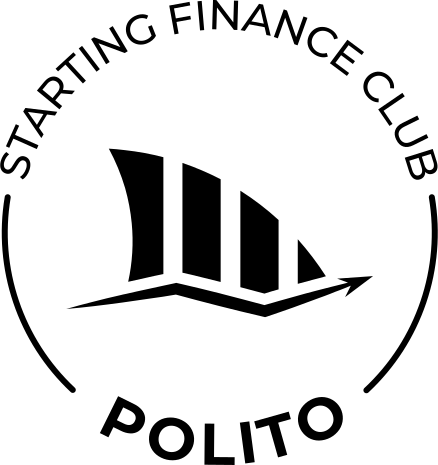
\includegraphics[width=1cm]{img/Logo_SFClub_Polito.png}}
\fancyfoot[C]{\thepage}
\renewcommand{\headrulewidth}{0.4pt}
\renewcommand{\footrulewidth}{0.4pt}
\setlength{\headheight}{25pt}
\setlength{\headsep}{24pt} % spazio sotto l'header

\fancypagestyle{plain}{%
  \fancyhf{}
  \fancyhead[L]{\textbf{Starting Finance Club PoliTo}}
  \fancyhead[R]{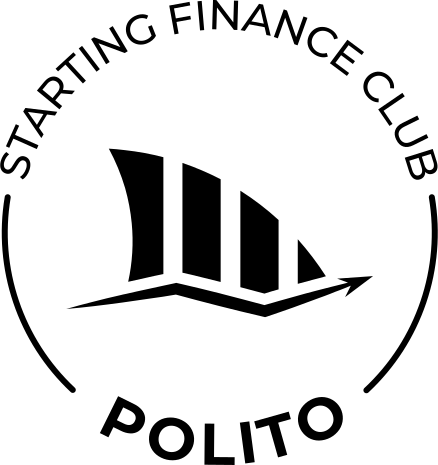
\includegraphics[width=1cm]{img/Logo_SFClub_Polito.png}}
  \fancyfoot[C]{\thepage}
  \renewcommand{\headrulewidth}{0.4pt}
  \renewcommand{\footrulewidth}{0.4pt}
}

% ===== Ambienti theorem ecc. =====
\theoremstyle{plain}\newtheorem{theorem}{Theorem}[chapter]
\theoremstyle{definition}\newtheorem{definition}{Definition}[chapter]
\newtheorem{notation}{Notation}[chapter]
\theoremstyle{remark}\newtheorem{remark}{Remark}[chapter]

\newenvironment{pseudocode}{\par\small\ttfamily\begin{adjustwidth}{1em}{1em}}{\end{adjustwidth}\par}

\newenvironment{tightabstract}[1][0.88]{%
  \begin{center}
  \begin{tcolorbox}[title={Abstract}, width=#1\textwidth, left=5mm, right=5mm,
    colback=white, boxrule=0.4pt]
  \small\justifying
}{%
  \end{tcolorbox}
  \end{center}
}

% Bibliography come chapter* + TOC + header

\makeatletter
\newenvironment{references}{%
  \chapter*{Bibliography}%
  \addcontentsline{toc}{chapter}{Bibliography}%
  \markboth{Bibliography}{Bibliography}%
  \list{\@biblabel{\@arabic\c@enumiv}}{%
    \settowidth\labelwidth{\@biblabel{99}}%
    \leftmargin\labelwidth
    \advance\leftmargin\labelsep
    \@openbib@code
    \usecounter{enumiv}%
    \let\p@enumiv\@empty
    \renewcommand\theenumiv{\@arabic\c@enumiv}}%
  \sloppy
  \clubpenalty4000
  \@clubpenalty\clubpenalty
  \widowpenalty4000
  \sfcode`\.\@m
}{%
  \def\@noitemerr{\@latex@warning{Empty `references' environment}}%
  \endlist
}
\makeatother

% ===== Fix capitoli: -18pt e dimensioni numeriche =====
\makeatletter
\patchcmd{\@makechapterhead}{\vspace*{50\p@}}{\vspace*{-18\p@}}{}{}
\patchcmd{\@makeschapterhead}{\vspace*{50\p@}}{\vspace*{-18\p@}}{}{}
\patchcmd{\@makechapterhead}{\huge}{\fontsize{17}{20}\selectfont\bfseries}{}{}
\patchcmd{\@makechapterhead}{\Huge}{\fontsize{20}{24}\selectfont\bfseries}{}{}
\patchcmd{\@makeschapterhead}{\Huge}{\fontsize{20}{24}\selectfont\bfseries}{}{}
\patchcmd{\@makechapterhead}{\vskip 20\p@}{\vskip 6\p@}{}{}
\patchcmd{\@makechapterhead}{\vskip 40\p@}{\vskip 10\p@}{}{}
\patchcmd{\@makeschapterhead}{\vskip 40\p@}{\vskip 10\p@}{}{}
\makeatother

% ===============================
\newcommand{\miniabstract}[1]{\begin{tcolorbox}[colback=gray!6,colframe=black!15,boxrule=0.3pt]\small\textit{Mini-abstract.} #1\end{tcolorbox}}

\usepackage[T1]{fontenc}
\usepackage{lmodern}
\usepackage{listings}
\usepackage{mathtools}
\usepackage{caption}
\usepackage{subcaption}
\usepackage[ruled,vlined]{algorithm2e}
\newcommand{\textcite}[1]{\cite{#1}}
\newcommand{\parencite}[1]{\cite{#1}}
\newtheorem{proposition}{Proposition}[chapter]
\newcommand{\E}{\mathbb{E}}
\newcommand{\Var}{\operatorname{Var}}
\newcommand{\Cov}{\operatorname{Cov}}
\newcommand{\R}{\mathbb{R}}
\newcommand{\dd}{\,\mathrm{d}}
\newcommand{\1}{\mathbf{1}}
\newcommand{\Texp}{\mathrm{T}}
\newcommand{\argmin}{\operatorname*{arg\,min}}
\newcommand{\safeincludegraphics}[2][]{\includegraphics[#1]{#2}}
\newcommand{\sourcecontext}[1]{\begin{tcolorbox}[colback=gray!5,colframe=gray!35,boxrule=.3pt]\small #1\end{tcolorbox}}

\begin{document}
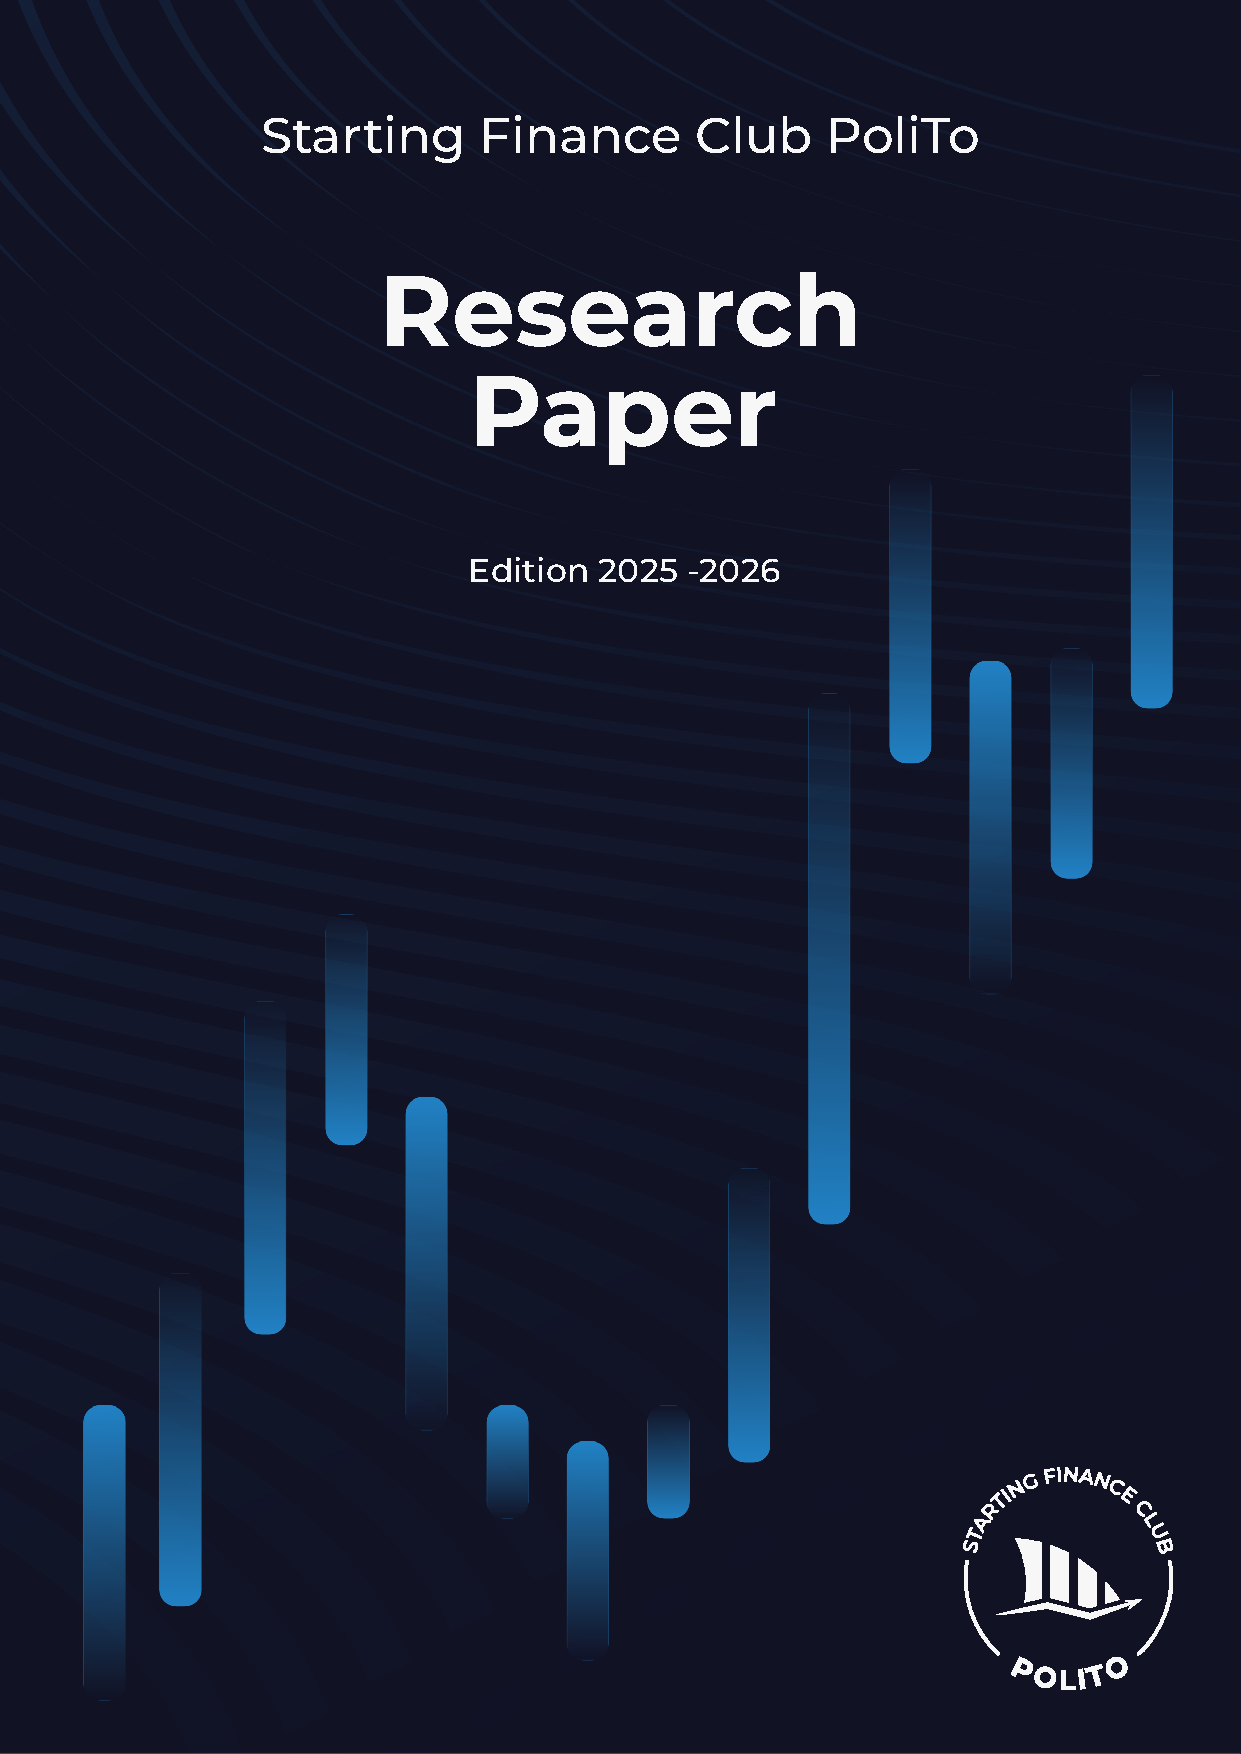
\includepdf[pages=1,fitpaper=true,pagecommand={\thispagestyle{empty}}]{Copertina_research.pdf}
\begin{titlepage}\thispagestyle{empty}\begin{center}
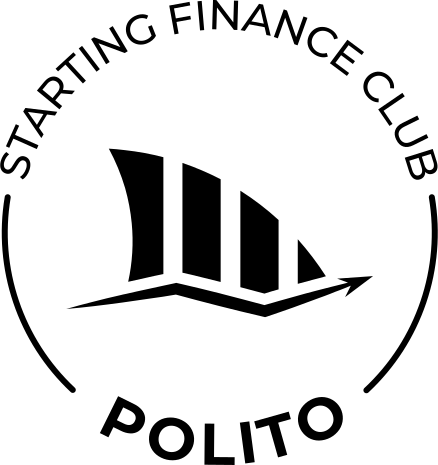
\includegraphics[width=2.4cm]{img/Logo_SFClub_Polito.png}\par\vspace{.7cm}
{\LARGE\bfseries High-Frequency Market Making:\\Models, Rough States and Numerical Control\par}\vspace{.3cm}
{\large Unified study\par}\vspace{.5cm}
Inventory control across Markovian and memory-dependent models\\
Original contributions: Salvatore Gabriele Messina and Niccol\`o Soriano (HFT1/HFT2); Salvatore Gabriele Messina (HFT3).\\[.3cm]
Revision: 13 October 2026. Publication date not assigned.\\[.4cm]
Starting Finance Club PoliTo\\
\url{https://github.com/StartingFinanceClubPoliTo/Research}
\end{center}\begin{tightabstract}We study one inventory-control problem across Markovian diffusions, non-Markovian memory drivers and finite Markovian lifts. Shared cash--inventory accounting connects the models, while their predictive states and approximation errors remain distinct. A common numerical framework compares classical quoting, historical scalar controls and a positive bounded-control baseline. In a synthetic two-asset experiment, a covariance proxy lowers accumulated price risk but lowers mean liquidated PnL and sample CARA certainty equivalent and increases the reconstructed full HJB residual. The evidence explains why inventory hedging, utility improvement and residual correction require separate checks. No fitted P3, exact memory-model solution, convergence certificate or latency advantage is claimed.\end{tightabstract}\end{titlepage}
\setcounter{tocdepth}{1}
\tableofcontents
\chapter{The Inventory Problem and the Information State}
\label{ch:common}
Market making poses one economic question throughout this study: how should executable bid and ask quotes trade spread revenue against inventory risk and terminal liquidation? We change the price and volatility state while keeping cash--inventory accounting explicit. The organizing distinction is the information needed to predict continuation risk, rather than the order in which the source manuscripts were written~\cite{hft1,hft2}.

\section{The predictive-state hierarchy}
ABM and GBM are Markovian price specifications. A correlated diffusion remains Markovian when its full price/inventory state is retained. Fractional and general Volterra drivers introduce memory; except in special kernels or the Brownian case, their current scalar value is insufficient for a recursive prediction. A finite exponential lift then constructs a \emph{new finite-dimensional Markovian model} that approximates the memory kernel. Compressing that lift into a scalar OU surrogate is a further approximation, not the same operation as lifting.

\begin{table}[htbp]\centering\small
\begin{tabularx}{\textwidth}{@{}p{.24\textwidth}p{.26\textwidth}X@{}}\toprule
Representation & Predictive state & What is gained or lost\\\midrule
ABM / GBM & Current price and inventory & Recursive diffusion benchmark; GBM reservation formula is local\\
Correlated diffusion & Price and inventory vectors & Cross-asset inventory risk; no volatility memory\\
Fractional / Volterra driver & Generally its relevant past or infinite state & Memory and causal kernels; no scalar Markov closure in general\\
Finite exponential lift & All OU factors and inventories & Finite Markov recursion; kernel approximation remains\\
Scalar OU surrogate & Aggregate volatility and inventory & Small HJB grid; full factor drift/diffusion need not match\\
Embedded / covariance proxy & Scalar policy evaluated on the lift & Cheap policy reuse; full residual and utility require separate checks\\\bottomrule
\end{tabularx}
\caption{The hierarchy used to connect the models. Markovianity refers to the retained state, not to a label attached to a historical experiment.}
\label{tab:model-hierarchy}
\end{table}

The mathematical development moves from the shared execution problem to diffusion models, then to non-Markovian memory, finite lifting and the full/reduced HJBs. One numerical-methods chapter explains simulation, positivity, export and the C++ operator. One results chapter then compares \emph{within} each experiment: the historical diffusion benchmark, three finite-lift configurations, a positive baseline and a two-asset covariance proxy. Their different terminal costs, path counts and solver conventions prevent a pooled performance ranking.

The principal intersection is covariance: it determines the classical portfolio-risk penalty, the memory driver's law, the OU innovation covariance and the full operator's mixed derivatives. These are different covariance objects. Keeping them distinct explains why an inventory hedge can lower accumulated price risk while worsening a full-state residual or failing to improve sample utility.
\section{Economic setting and notation}

This paper studies the interface between market making and market microstructure through the lens of two time scales. At the daily scale, an asset price can be idealized as a continuous-time process (e.g., a Brownian-motion-like mid-price), and the market maker's problem resembles dynamic risk management with the objective of harvesting the bid--ask spread while controlling inventory exposure. At the sub-second scale, the same environment becomes intrinsically discrete and rule-driven: prices live on a tick grid, orders arrive asynchronously, and the limit order book mechanics and trading frictions shape both the observed price formation and the feasibility of any quoting strategy. The core message is that market making cannot be fully understood at only one resolution: a smooth diffusion view is useful for tractability and control, while a microstructural view is essential for interpreting what the mid-price represents and for implementing strategies under real trading constraints.

Within this perspective, market making can be summarized as an algorithmic decision rule that continuously updates bid and ask quotes as a function of a state vector. Conceptually, the market maker forms a (possibly personal) estimate of value and quotes around it, posting a bid below and an ask above, then adapts these quotes as the state changes, most importantly as the mid-price moves and inventory accumulates. The economic role of this activity is liquidity provision: by standing ready to trade on both sides, the market maker supplies immediacy to other market participants who value execution without delay.

Historically, the intuition of a two-sided quote originated in floor-based settings with designated dealers (often specialists) who were central to trading in a given name. Modern electronic markets replace this institutional structure with competitive, automated quoting in data-center environments, where many agents simultaneously post and cancel orders at high frequency. This evolution motivates the academic progression from classical inventory-based dealer models, built around utility maximization and Hamilton--Jacobi--Bellman (HJB) equations, to electronic-market approximations that yield implementable quoting formulas and accommodate realistic constraints such as inventory bounds, risk limits, adverse selection, and multi-asset interactions.

Against this background, the Avellaneda--Stoikov paradigm provides a canonical benchmark: it formalizes the idea that the market maker effectively buys low and sells high, but on compressed horizons (seconds or minutes rather than days), and it makes explicit how optimal spreads and skew depend on inventory risk and order arrival dynamics. The goal of this paper is to apply this inventory-based logic across alternative stochastic specifications for the underlying state variables (different mid-price dynamics and a covariance-aware multivariate inventory state), while keeping the economic mechanism invariant: the market maker controls quotes to balance spread capture against inventory and execution risk under microstructural frictions.

\subsection{Notation}
\begin{tabularx}{\textwidth}{@{}lX@{}}
\toprule
$S_t$ & Mid-price / reference price \\
$q_t$ & Inventory (number of shares/contracts) \\
$X_t$ & Cash account \\
$W_t$ & Total wealth / overall P\&L \\
$\delta_t^{bid}, \delta_t^{ask}$ & Distance from the mid-price for bid/ask quotes \\
$p_t^{bid}, p_t^{ask}$ & Quoted prices (bid/ask) \\
$\lambda^{bid}(\delta), \lambda^{ask}(\delta)$ & Arrival intensities of market orders hitting the bid/ask quotes \\
$N_t^{bid}, N_t^{ask}$ & Counting processes of fills at the bid/ask \\
$\sigma$ & Volatility / instantaneous scale \\
$\gamma$ & Risk aversion (CARA / exponential utility) \\
$T$ & Policy horizon \\
$\Delta t$ & Simulation time step \\
\bottomrule
\end{tabularx}

With this notation fixed, the first substantive chapter turns to the institutional and microstructural environment in which these variables acquire meaning. The goal is to move from the abstract state variables used later in the stochastic-control model to the concrete LOB mechanics, order types, and HFT risks that motivate the Avellaneda--Stoikov benchmark.
\section{Market Microstructure and High-Frequency Trading: LOB Foundations, Taxonomy, and Risks}
\label{hft1-ch:microstructure_hft}


\subsection{LOB Mechanics}
Modern electronic equity and crypto venues are typically organized as continuous double auctions implemented through a limit order book (LOB). At any time $t$, the book aggregates standing intentions to buy and sell. The best available buy price is the \emph{best bid} $p_t^{bid}$ and the best available sell price is the \emph{best ask} $p_t^{ask}$. The \emph{bid--ask spread} is
\[
\mathrm{spr}_t = p_t^{ask}-p_t^{bid},
\]
and a standard reference price is the \emph{mid-price}
\[
S_t=\frac{p_t^{ask}+p_t^{bid}}{2}.
\]
In practice, $S_t$ is an informational proxy rather than a traded price: executions occur at discrete prices on the book, while $S_t$ is a convenient state variable used to define quote distances $\delta_t^{bid},\delta_t^{ask}$ and to mark-to-market total wealth $W_t$ in reduced-form models.

A central microstructural friction is price discreteness. Exchanges impose a \emph{tick size} $\tau>0$, meaning that admissible prices lie on a grid (multiples of $\tau$). Tick size interacts with quoting and execution probability: for a given $S_t$, a one-tick change in $p_t^{bid}$ or $p_t^{ask}$ may cause a discontinuous jump in competitiveness and thus in expected fills.

The depth of the book describes how many shares/contracts are available at each price level. If $D_t^{bid}(p)$ denotes cumulative buy depth at prices $\ge p$ and $D_t^{ask}(p)$ cumulative sell depth at prices $\le p$, then the slope of these curves around the top of book summarizes local liquidity. Depth matters because it shapes the impact of market orders, the stability of the top quotes, and the typical waiting time for a new limit order to be executed.

Finally, most venues implement price-time priority. Orders at better prices execute first. Among orders at the same price, earlier arrivals have priority. This induces queueing: a market maker who posts at the best bid or ask typically joins a queue, and the probability of being filled depends not only on the level of $p_t^{bid}$ or $p_t^{ask}$ but also on queue position. These mechanics are key for realistic implementation, even when the analytical model abstracts them into a reduced-form \emph{arrival intensity} $\lambda^{bid}(\delta)$ and $\lambda^{ask}(\delta)$ that depends only on the distance $\delta$ from $S_t$. Standard treatments of these concepts can be found in classical market microstructure references such as \textcite{OHara1995}, \textcite{Harris2003}, and \textcite{Hasbrouck2007}.

\subsection{Orders and Order Flow}
LOB dynamics are driven by the interaction of different order types. A limit order specifies a side (buy/sell), a price, and a quantity, and provides liquidity by adding depth to the book. A market order consumes liquidity by executing immediately against the standing best quote(s), walking the book if its size exceeds the available top-of-book depth.

A key empirical feature is that books are highly dynamic because orders are frequently cancelled or modified. Cancellations are essential for market making: when $S_t$ moves or $q_t$ changes, a market maker typically cancels stale quotes and reposts new ones. From a modeling perspective, cancellations generate a high-frequency churn that affects queue position and realized execution rates. In reduced-form models, their net effect is often captured through effective \emph{fill processes} $N_t^{bid}$ and $N_t^{ask}$ with intensities $\lambda^{bid}(\cdot)$ and $\lambda^{ask}(\cdot)$.

Executions can also be partial. When a market order hits a limit order of size larger than the incoming quantity, only a portion is executed and the remaining quantity stays in the book, preserving price-time priority at that level. Conversely, if a market order size exceeds top depth, it consumes multiple levels and produces immediate changes in $p_t^{bid}$ and $p_t^{ask}$, which in turn shift $S_t$.

Latency is another structural element. There is always a non-zero delay between observing the state of the book and having a cancel/replace action acknowledged by the exchange. During this window, an HFT market maker is exposed to adverse price movements and unexpected executions at quotes that were intended to be updated. In practice, latency and message processing limits shape optimal quoting, but in baseline Avellaneda--Stoikov-type models they are typically abstracted away so that quotes can be treated as continuously adjustable. The resulting model should thus be interpreted as an idealized benchmark rather than a full description of the LOB.

These ingredients motivate the modeling choice adopted later: rather than simulating the entire queue and message flow, we represent executions by counting processes $N_t^{bid},N_t^{ask}$ whose conditional intensities $\lambda^{bid}(\delta)$ and $\lambda^{ask}(\delta)$ depend on how far the quotes are from the reference mid-price $S_t$. This captures the first-order trade-off faced by a liquidity provider: tighter $\delta_t^{bid},\delta_t^{ask}$ increase expected fills and spread capture, but also increase exposure to inventory risk through $q_t$ and to execution risk through random fill timing.

\subsection{Empirical Stylized Facts and Reduced-Form Book Models}
Empirical work on limit order books documents robust regularities across assets and venues. One such regularity is order book imbalance: when buy-side depth near the top of book exceeds sell-side depth (or vice versa), short-term price moves tend to be biased toward the thinner side. Imbalance provides a microstructural signal that can be used to tilt quoting or control inventory, although incorporating it explicitly requires either book data or a structural model for depth dynamics.

A second feature is resilience: after liquidity is consumed by aggressive orders, the book tends to replenish over time through new limit orders and cancellations. Resilience determines how quickly spreads revert and how persistent the impact of temporary shocks is. For market makers, low resilience increases the risk of being caught with inventory $q_t$ during sustained adverse moves in $S_t$, while high resilience improves the ability to mean-revert $q_t$ through subsequent fills.

A third feature is clustering in order flow. Trades and order submissions are not independent in time; instead, they arrive in bursts. This motivates models beyond homogeneous Poisson processes, such as self-exciting point processes, which can reproduce clustered arrivals and endogenous fluctuations in execution intensity. However, these richer specifications complicate both analysis and calibration.

Tick size discreteness creates additional effects. When $\tau$ is large relative to typical short-term volatility $\sigma_t$, the top of book may be relatively stable and market makers can earn the spread more reliably. When $\tau$ is small, competition tightens spreads and queueing becomes more relevant. In both cases, tick constraints imply that the mapping from a continuous reference $S_t$ to admissible quotes is quantized, which can be important when interpreting theoretical optimal $\delta_t^{bid},\delta_t^{ask}$ in implementation.

Comprehensive surveys of empirical LOB properties and modeling approaches are provided in \textcite{GouldEtAl2013}. In the present work, we intentionally adopt a reduced-form execution model for comparability across mid-price specifications: the execution mechanism (counting processes $N_t^{bid},N_t^{ask}$ with intensities $\lambda^{bid}(\cdot),\lambda^{ask}(\cdot)$) is held fixed while the mid-price dynamics are varied under a common finite-horizon design. This choice isolates the effect of the price model on inventory-based control. Imbalance, resilience, order-flow clustering, queue position, and latency are discussed as economically relevant LOB mechanisms, but they are not state variables in the benchmark simulator and they are natural extensions beyond the baseline model.

\subsection{High-Frequency Trading: Operational Definitions and Key Metrics}
High-frequency trading (HFT) refers to algorithmic strategies that operate on short horizons, where the interaction between trading decisions and market microstructure becomes first-order. In this context, the \emph{policy horizon} $T$ is not only a modeling choice but an operational constraint: strategies are designed to make decisions and manage risk over seconds, milliseconds, or even microseconds, and their profitability depends on how quickly they can adapt to changing order flow and movements in the reference price $S_t$.

As seen in the previous section, a central metric is latency, broadly defined as the end-to-end delay between (i) observing a market state and (ii) having an action (e.g., a new quote, a cancel/replace, or a hedge) acknowledged and made effective by the venue. Latency can be decomposed into data latency, decision latency, and execution latency. In market making, latency directly impacts the ability to maintain intended quote distances $\delta_t^{bid},\delta_t^{ask}$ and inventory targets for $q_t$, and it creates exposure to fills at stale quotes, thereby affecting the realized dynamics of $N_t^{bid}$ and $N_t^{ask}$.

Turnover measures how frequently capital is recycled. At the strategy level, it is commonly proxied by traded volume relative to a notional base, and at the position level it is related to the rate at which $q_t$ mean-reverts. High turnover is not automatically desirable: it may increase gross spread capture, but it can also amplify transaction costs, queue losses, and exposure to toxic flow.

Because HFT operates at the micro scale, practitioners rely on micro-signals and liquidity indicators that summarize the state of the book and recent order flow. Typical examples include the spread $\mathrm{spr}_t$ and top-of-book depth, imbalance, recent trade signs and intensities, short-term realized volatility, and measures of flow persistence. These features are used either to tilt quoting (in market making), to time entry/exit (in arbitrage or stat-arb), or to control urgency and slippage (in execution). In this paper, we keep the execution model reduced-form and let liquidity conditions primarily enter through the parameters governing $\lambda^{bid}(\delta),\lambda^{ask}(\delta)$ and through the volatility scale $\sigma$.

\subsection{Classes of Strategies}
HFT is best viewed as a family of strategies rather than a single paradigm. The common thread is fast reaction to market conditions, but objectives and risk exposures differ substantially across classes.

\paragraph{Market making (core of this work).}
A market maker supplies liquidity by posting bid and ask quotes and earns the spread conditional on being filled. The defining risk is inventory: if buys and sells do not balance, the market maker accumulates an inventory $q_t$ that is exposed to movements in $S_t$. In reduced-form models, the strategy controls the trade-off between execution probability and risk by adjusting quote distances $\delta_t^{bid},\delta_t^{ask}$ from the reference mid-price $S_t$. The present work treats market making as a controlled quoting problem, comparing a naive symmetric policy to an inventory-aware policy derived from the Avellaneda--Stoikov principle.

\paragraph{Statistical arbitrage and cross-venue trading (operational context).}
Statistical arbitrage encompasses strategies that exploit temporary mispricings across related instruments (pairs or baskets) or across venues. In a cross-venue setting, the strategy may buy on one venue and sell on another to capture price differentials, subject to latency, fees, and execution risk. In a related-instruments setting, the strategy may trade a spread or mean-reverting residual, requiring careful control of model risk and regime changes. These strategies share important infrastructure with market making (low-latency execution, queue management, and robust risk controls) but their alpha mechanism is typically driven by relative value rather than spread capture.

\paragraph{Execution and optimal execution (comparison baseline).}
Execution algorithms aim to trade a given quantity while minimizing cost and risk, rather than to provide liquidity continuously. The objective is typically a functional of expected slippage, volatility risk, and market impact, leading to policies that schedule participation rates or adaptively vary urgency over time. Classical frameworks formalize this problem using stochastic control and dynamic programming (see \textcite{CarteaJaimungalPenalva2015}). Execution provides a useful contrast to market making: in market making the trader chooses quotes to be hit, whereas in execution the trader chooses aggressiveness to achieve a target quantity, often paying the spread instead of earning it.

\subsection{Risks and Constraints}
Although HFT strategies can be framed as optimization problems, real-world performance is shaped by risks and constraints that may not be fully captured by baseline models. For market making, these risks motivate the inventory-aware structure studied later.

\paragraph{Inventory risk.}
Inventory risk is the exposure of the dealer's position to price movements. In the Avellaneda--Stoikov setting, inventory enters the objective through marked-to-market wealth $W_t$ and is controlled via quote skew: the market maker shifts $\delta_t^{bid}$ and $\delta_t^{ask}$ to encourage trades that reduce $q_t$. Inventory limits (hard bounds) and risk budgets (soft penalties) are standard constraints in practice.

\paragraph{Adverse selection and toxicity.}
Adverse selection occurs when incoming market orders are informational: the market maker sells just before $S_t$ rises or buys just before $S_t$ falls. This is often described as toxic flow, because it turns apparent spread revenue into losses. In reduced-form models, adverse selection can be approximated by state-dependent intensities $\lambda^{bid}(\cdot),\lambda^{ask}(\cdot)$ or by coupling executions to future changes in $S_t$, but fully modeling it typically requires richer microstructure inputs. In the simulations below, adverse selection and toxicity are not modeled explicitly, but they remain risk channels that the benchmark abstracts away.

\paragraph{Queue risk.}
When quotes are placed at competitive prices, fills depend on queue position at $p_t^{bid}$ and $p_t^{ask}$. Frequent cancellations and reposting may improve alignment with $S_t$ but can worsen priority. Thus, there is a trade-off between staying ``fresh'' and maintaining queue position. Queue risk is particularly important in low-volatility regimes where many market makers crowd the top of book and marginal priority determines realized fill rates for $N_t^{bid}$ and $N_t^{ask}$.

\paragraph{Latency and implementation risk.}
Latency creates a gap between intended and realized control. During delays, the strategy may be executed at stale quotes, miss hedges, or experience rapid changes in $q_t$. Additional implementation constraints include exchange message limits, minimum resting times, order throttles, and fees/rebates structures that can materially alter optimal quoting behavior.

\paragraph{Regime shifts and model risk.}
HFT strategies are sensitive to regime changes in volatility, liquidity, and order flow. A regime shift can invalidate parameters that were stable in calm periods (e.g., the effective intensity scale in $\lambda^{bid}(\cdot),\lambda^{ask}(\cdot)$ or the volatility level $\sigma$), causing abrupt changes in fill rates and inventory dynamics.

\subsection{Bridge to Avellaneda--Stoikov}
The discussion above provides the minimum context needed to motivate the Avellaneda--Stoikov benchmark. The LOB supplies the two-sided quoting mechanism through $p_t^{bid},p_t^{ask}$ around a reference $S_t$, order flow and cancellations motivate a reduced-form execution model in terms of fill processes $N_t^{bid},N_t^{ask}$ and intensities $\lambda^{bid}(\cdot),\lambda^{ask}(\cdot)$ and HFT metrics and risks clarify why inventory-aware control of $q_t$ and robustness across regimes are central. With this foundation, we now introduce Avellaneda--Stoikov as a tractable stochastic control formulation of market making and use it as the baseline engine for the simulation-based comparisons developed in the remainder of the work.

\section{High-Frequency Trading in a Limit Order Book: Core Ideas Behind Avellaneda--Stoikov}
\label{hft1-sec:hft_lob_core_ideas}


\subsection{Problem statement: how does a market maker create a bid--ask?}
The central question is: \emph{how can a market maker (MM) generate bid and ask quotes in a limit order book?} The MM provides liquidity by continuously posting a two-sided market, aiming to profit from spread capture while controlling the risks induced by random price fluctuations and random execution timing.

Two main sources of uncertainty drive the problem. First, there is inventory risk, stemming from the stochastic nature of the reference (mid) price process: if the MM accumulates inventory $q_t$, the marked-to-market value of that inventory fluctuates randomly with $S_t$. Second, there is transaction risk, due to the randomness in both the number of market orders and their arrival times: executions occur at random instants, and the MM cannot perfectly control when (and how often) its quotes are hit. The goal is therefore to choose a quoting policy that maximizes the MM's objective, formulated as utility maximization.

\subsection{Symmetric and Inventory-Sensitive Quoting}
A convenient way to organize the discussion is to contrast two approaches.

The first approach is a naive symmetric strategy. The MM posts a bid and an ask that are symmetric around the mid-price and do not depend on inventory. In other words, the distances from the mid-price are fixed (or exogenously time-dependent) and ignore the state variable $q_t$. This policy can capture spread revenue, but it does not actively control inventory risk: any inventory stabilization occurs only indirectly (e.g., through reduced fill rates when quoting wider).

The second approach is an inventory-based strategy: the MM calibrates its bid-ask quotes to the current inventory so as to push $q_t$ back toward $0$ by the end of the horizon. The key conceptual workflow is a two-step procedure. In Step~1, one computes an indifference price (or reservation price) that depends on inventory. In Step~2, one constructs bid and ask quotes around that inventory-dependent reference and calibrates their aggressiveness using the book/execution mechanism, typically summarized by arrival intensities.

\subsection{Minimal building blocks: price dynamics, order arrivals, and order sizes}
Even in a reduced-form model, the market-making problem requires three minimal blocks.

\paragraph{Mid-price dynamics.}
The reference price $S_t$ must be modeled, together with its volatility structure. Classical specifications use Brownian/It\^o diffusions, while richer specifications use Volterra-type dynamics or rough volatility drivers. Changing the dynamics of $S_t$ changes optimal quoting because it changes the distribution of future price moves and therefore the risk of holding inventory.

\paragraph{Order arrival mechanism.}
Executions are modeled via point processes (often Poisson in the baseline). A common reduced-form assumption is that the arrival intensity of market orders hitting the MM quotes depends on the quote distance from the mid-price. In notation consistent with the rest of the manuscript, one often writes effective intensities
\[
\lambda^{bid}(\delta), \qquad \lambda^{ask}(\delta),
\]
where $\delta$ represents the distance of the quote from $S_t$ (e.g., $\delta_t^{bid}$ or $\delta_t^{ask}$). The fill events are then summarized by counting processes $N_t^{bid}$ and $N_t^{ask}$.

\paragraph{Order size specification.}
One must specify the size of executions. In many baseline treatments, execution size is simplified to one unit per fill, which yields an inventory jump of $\pm 1$ at each execution. More general frameworks treat order sizes as random marks (marked point processes), which is more realistic but also more complex.

A practical remark is that under rough volatility or Volterra-type models, the volatility forecast over the relevant horizon $\sigma_t$ is no longer well-described by a constant (or even Markovian) but it varies over time. This changes how aggressively the MM must move quotes in response to inventory: when short-horizon volatility is clustered and persistent, inventory control often requires more state-dependent and regime-sensitive adjustments.

\subsection{A baseline mid-price model and CARA utility: why closed forms appear}
To illustrate how the indifference-price logic arises, consider a baseline specification where the mid-price follows an arithmetic Brownian motion with constant volatility. Specifically, assume that, for $u\ge t$,
\[
dS_u = \sigma\, dW_u,
\qquad S_t=s,
\]
where $W$ is a one-dimensional Brownian motion and $\sigma$ is constant. The modeling implication is that we impose no structure on drift or autocorrelation beyond this diffusion assumption. In particular, there is no attempt to encode predictability in $S_t$.

The objective is to maximize the exponential utility of terminal P\&L at a finite horizon $T$, i.e., a CARA (constant absolute risk aversion) preference with risk-aversion parameter $\gamma>0$. Exponential utility also connects naturally to convex risk measures and provides a clean framework for defining indifference prices.

As a first step, consider a frozen-inventory thought experiment in which the inventory is held fixed at level $q$ between $t$ and $T$. The associated value is
\[
v(x,s,q,t)
=
\mathbb{E}_t\!\left[-\exp\!\left(-\gamma\bigl(x+qS_T\bigr)\right)\right],
\]
where $x$ denotes initial wealth at time $t$, $s$ is the current mid-price $S_t$, and $q$ is the number of shares held. The parameter $\gamma$ quantifies risk aversion: increasing $\gamma$ makes the agent more risk averse (larger penalty for variance), while decreasing $\gamma$ moves the agent closer to risk neutrality.

Under arithmetic Brownian motion,
\[
S_T = s + \sigma\bigl(W_T-W_t\bigr),
\]
and conditioning on $\mathcal{F}_t$ yields
\[
\mathbb{E}_t[S_T]=s,
\qquad
\mathrm{Var}_t(S_T)=\sigma^2(T-t).
\]
Define terminal wealth
\[
Y:=x+qS_T.
\]
Then
\[
\mathbb{E}_t[Y]=x+qs,
\qquad
\mathrm{Var}_t(Y)=q^2\sigma^2(T-t).
\]
Using the standard Gaussian moment generating identity, if $Y\sim N(m,v)$ then 
\begin{align*}
    \mathbb{E}(e^{aY})=\exp(am+\tfrac12a^2v)
\end{align*}
with $a=-\gamma$, one obtains
\[
\mathbb{E}_t\!\left[-e^{-\gamma Y}\right]
=
-\exp\!\left(
-\gamma\,\mathbb{E}_t[Y]
+\frac12\gamma^2\,\mathrm{Var}_t(Y)
\right)
=
-\exp\!\left(
-\gamma(x+qs)
+\frac12\gamma^2 q^2\sigma^2(T-t)
\right).
\]
Equivalently, by splitting exponentials,
\[
v(x,s,q,t)
=
-\exp(-\gamma x)\,
\exp(-\gamma q s)\,
\exp\!\left(\frac{\gamma^2 q^2 \sigma^2 (T-t)}{2}\right).
\]
This factorization is particularly clean because the terminal wealth is Gaussian under ABM and the exponential utility interacts well with Gaussian mgfs. If instead $S_t$ followed GBM, such a neat factorization generally does not appear.

This ``closed-form friendliness'' is a direct consequence of the CARA/exponential specification $U(w)=-e^{-\gamma w}$: under normality (or more generally whenever the relevant moment generating function exists in a tractable form) computations simplify substantially. In Black--Scholes, for instance, $S_t$ is lognormal and expectations of the form $\mathbb{E}\bigl[-e^{-\gamma q S_T}\bigr]$ can be interpreted via Laplace-transform-type objects. For rough or otherwise more complex models, closed forms are typically lost and one must either (i) formulate and solve the associated Hamilton--Jacobi--Bellman (HJB) equation when the control is continuous, (ii) rely on numerical methods/simulation to approximate the value function, or (iii) modify the objective (e.g., mean--variance criteria or utilities on transformed prices such as log-prices).

Importantly, in more complex, non-Gaussian diffusion models, closed forms are typically lost but the qualitative dependence between optimal bid--ask placement and inventory remains. What changes is the computation: in Gaussian settings one obtains closed forms and ``clean'' separability, while in more realistic settings the inventory correction typically becomes a function of the full state (e.g., $s,q,t,\text{volatility},\text{other states}$) because both risk and the future distribution of $S_t$ depend on those factors. Operationally, the optimality conditions may be expressed in terms of partial derivatives of the value function, which are difficult to obtain in high-dimensional HJB/PDE problems and therefore motivate numerical schemes.

\subsection{Reservation prices via indifference: finite horizon}
The key quantity in inventory-based quoting is the \emph{reservation price} (indifference price): the price that makes the agent indifferent between keeping the current portfolio and switching to a portfolio with one more (or one fewer) share.

Formally, define the reservation bid price $r^b(s,q,t)$ and reservation ask price $r^a(s,q,t)$ as the solutions to
\[
v\bigl(x-r^b(s,q,t),\,s,\,q+1,\,t\bigr)=v(x,s,q,t),
\qquad
v\bigl(x+r^a(s,q,t),\,s,\,q-1,\,t\bigr)=v(x,s,q,t).
\]
Under the ABM--CARA frozen-inventory expression above, these conditions yield
\[
r^b(s,q,t)
=
s+(-1-2q)\,\frac{\gamma\sigma^2(T-t)}{2},
\qquad
r^a(s,q,t)
=
s+(1-2q)\,\frac{\gamma\sigma^2(T-t)}{2}.
\]
A convenient reference is the ``center'' reservation level (the midpoint between reservation bid and ask),
\[
r(s,q,t)
=
\frac12\bigl(r^a(s,q,t)+r^b(s,q,t)\bigr)
=
s-\,\gamma q\sigma^2(T-t).
\]
This expression highlights the inventory effect: if the agent is long stock ($q>0$), then $r(s,q,t)$ lies below the mid-price, meaning the agent is willing to sell at a lower price to reduce inventory. If the agent is short ($q<0$), then $r(s,q,t)$ lies above the mid-price, meaning the agent is willing to buy back at a higher price to close the short position.

In this paper, the reservation-price construction is kept in its finite-horizon form. This is sufficient for the ABM and GBM simulation benchmarks and keeps the terminal-wealth criterion consistent across the single-asset models.

The reservation-price step above provides the first half of the Avellaneda--Stoikov logic. The second half connects reservation prices to actual bid-ask quotes by incorporating execution probabilities through $\lambda^{bid}(\cdot)$ and $\lambda^{ask}(\cdot)$, i.e., by choosing quote distances that trade off fill rates against inventory and price risk. This connection is developed in the subsequent Avellaneda--Stoikov section.

\subsection{Market Making as a Liquidity Provision Problem}
A market maker provides immediacy by standing ready to buy and sell. If the dealer posts a bid below the current reference price and an ask above it, profits arise when both sides are hit over time and the spread is captured. However, the execution of the two sides is random. If the dealer buys repeatedly without selling, inventory builds up; if the price then falls, marked-to-market wealth deteriorates. Inventory control is therefore central to market making, especially on short horizons where positions can grow quickly relative to the dealer's risk budget.

Historically, two-sided quoting was associated with designated specialists or dealers on centralized exchanges. In modern electronic markets, the same economic function is carried out by many competing agents that post and cancel orders at high frequency. This institutional evolution is why reduced-form models of quoting, execution intensities, and inventory risk remain valuable: they transform a complex market mechanism into a control problem with clear state variables and interpretable parameters.

The following state-dynamics discussion converts this economic intuition into the formal Avellaneda--Stoikov framework. We move from the qualitative description of two-sided liquidity provision to explicit state dynamics, fill intensities, and a finite-horizon utility objective that can be solved through dynamic programming.

\section{The Avellaneda--Stoikov Framework}


\subsection{State Dynamics}
The state of the MM is fully characterized by the triad $(S_t, q_t, X_t)$, representing respectively the reference mid-price, the current inventory (number of shares/contracts), and the cash account. The dealer provides liquidity by posting quotes at distances $\delta_t^{bid}$ and $\delta_t^{ask}$ from the mid-price
\[
p_t^{bid}=S_t-\delta_t^{bid}, \qquad p_t^{ask}=S_t+\delta_t^{ask},
\]
with $\delta_t^{bid},\delta_t^{ask}\ge 0$.

It is crucial to distinguish the continuous nature of the price from the discrete nature of the dealer's accounting. Assuming unit trade sizes, the executions are modeled via the counting point processes $N_t^{bid}$ and $N_t^{ask}$. Consequently, inventory and cash are jump processes that evolve only when an order is filled
\begin{align*}
    &dq_t=dN_t^{bid}-dN_t^{ask},\\
    &dX_t=(S_t+\delta_t^{ask})\,dN_t^{ask}-(S_t-\delta_t^{bid})\,dN_t^{bid}.
\end{align*}
Economically, when a market seller hits the bid ($dN_t^{bid}=1$), the dealer buys one share (increasing $q_t$) and pays the bid price (decreasing $X_t$). Conversely, a fill at the ask ($dN_t^{ask}=1$) reduces inventory and increases cash.

The continuous performance of the strategy is measured by the total wealth at any time $t$
\[
W_t=X_t+q_tS_t.
\]
This equation encapsulates the core of the market making problem. While the accumulated cash $X_t$ is insulated from price movements, the portfolio value $q_tS_t$ is continuously exposed to the stochastic fluctuations of $S_t$. The terminal objective evaluated at the policy horizon $T$ is based on 
\[
W_T=X_T+q_TS_T,
\]
driving the need for an optimal control policy that balances the spread capture in $X_t$ against the inventory risk inherent in $q_tS_t$.

\subsection{Arrival Intensities}
To close the specification of the state dynamics, we must define the behavior of the counting processes $N_t^{bid}$ and $N_t^{ask}$. The dealer does not have direct control over when an execution occurs, but they control the probability of an execution by choosing the quotation distances $\delta_t^{bid}$ and $\delta_t^{ask}$.

Let $\lambda(\delta)$ denote the arrival rate (intensity) of filled limit orders at a distance $\delta$ from the mid-price. Following the specific framework proposed by Avellaneda and Stoikov, we assume that the arrival of executions depends on three main market components:
\begin{enumerate}
    \item The overall constant frequency of market orders (liquidity-taking orders), denoted by $\Lambda$;
    \item The distribution of the volume size $Q$ of these market orders, which is empirically shown to follow a power law density $f^Q(x) \propto x^{-1-\alpha}$;
    \item The temporary market impact $\Delta p$ caused by a large market order.
\end{enumerate}
If a market order creates a temporary price impact $\Delta p$, the dealer's limit order posted at a distance $\delta$ will be executed only if the impact is large enough to reach the quote, i.e., if $\Delta p>\delta$. Therefore, the execution intensity is proportional to the probability of this event.

Following the finding that the price impact of an order of size $Q$ is best described by a logarithmic function 
\[
\Delta p \propto \ln{(Q)} 
\]
we can derive the exact functional form for the arrival intensity as follows
\begin{align*}
    \lambda(\delta)&=\Lambda \mathbb{P}(\Delta p>\delta)=\\
    &=\Lambda \mathbb{P}(\ln{(Q)}>K\delta)=\\
    &=\Lambda \mathbb{P}(Q>e^{K\delta})=\\
    &=\Lambda \int_{e^{K\delta}}^{+\infty}x^{-1-\alpha}dx= Ae^{-k\delta},
\end{align*}
where the constants are redefined as $A = \Lambda /\alpha$ and $k=\alpha K$.

This result provides us with the exponential intensities for the bid and ask sides
\[
\lambda^{ask}(\delta)=Ae^{-k\delta}, \qquad \lambda^{bid}(\delta)=Ae^{-k\delta}.
\]
In this reduced-form representation, the parameter $A$ retains the interpretation of the base market activity (the arrival rate at the mid-price), while $k$ controls execution sensitivity to quote aggressiveness. A larger $k$ means that the execution intensity decays more rapidly as the dealer moves quotes away from the mid-price. This dynamic establishes the core trade-off of the market making problem: quoting further away secures a larger margin per trade but exponentially dampens the execution probability.

\subsection{Objective Function}
Having established the dynamics of the state variables and the microstructural mechanics of order executions, we now formalize the dealer's objective. The market maker seeks to maximize the expected utility of their terminal wealth at a fixed horizon $T$ (e.g., the end of the daily trading session). Let 
\[
W_T = X_T + q_TS_T
\]
denote the marked-to-market wealth at the terminal time $T$. To rigorously capture the dealer's aversion to inventory risk, the optimization is cast within an expected utility framework using a Constant Absolute Risk Aversion (CARA) utility function
\[
u(W_T) = -e^{-\gamma W_T} 
\]
where $\gamma>0$ is the absolute risk aversion coefficient. The choice of the exponential utility is not merely mathematically convenient, it economically reflects the dealer's penalization of wealth variance. Since the cash account is riskless, the variance of the terminal wealth is entirely driven by the inventory position $q_T$ exposed to the price volatility $\sigma$.

The market maker's problem consists of finding the optimal predictable quoting policies (the controls), $\delta_t^{bid}$ and $\delta_t^{ask}$, that maximize the expected terminal utility conditional on the state at time $t$. We define the value function $u(t,S_t ,q_t, X_t)$ as
\begin{align*}
    u(t,s,q,x)&=\max_{\{\delta_t^{bid},\delta_t^{ask}\}_{t\in[0,T]}} \mathbb{E}\left[-\exp\!\left(-\gamma W_T\right)|S_t=s,q_t=q,X_t=x\right]=\\
    &=\max_{\{\delta_t^{bid},\delta_t^{ask}\}_{t\in[0,T]}} \mathbb{E}_t\left[-\exp\!\left(-\gamma (X_T+q_TS_T)\right)\right].
\end{align*}
This formulation represents a classic finite-horizon stochastic optimal control problem. Exponential utility is convenient because it interacts well with Gaussian benchmark models and yields interpretable reservation-price formulas \cite{AvellanedaStoikov2008}, \cite{GueantLehalleFernandezTapia2013}.

Having formally defined the stochastic control problem and demonstrated the wealth-independence of the quoting strategy, the next step is to derive the optimal controls $\delta_t^{bid}$ and $\delta_t^{ask}$. This requires solving the dynamic programming problem through its associated Hamilton-Jacobi-Bellman (HJB) equation, which we establish in Chapter~\ref{ch:markov}.

The execution and utility conventions established here stay fixed when possible. The next chapter changes the diffusion specification and inventory dimension; later chapters change the volatility information state. A result for one of these models does not automatically transfer to another.

\chapter{Markovian Diffusions and Inventory-Sensitive Quotes}\label{ch:markov}
With the economic objective fixed, the simplest predictive state is the current diffusion price and inventory. We first derive the CARA quoting mechanism, then distinguish additive ABM, multiplicative GBM and correlated multi-asset risk. These formulas provide the benchmark against which memory and state compression will be interpreted.
\section{Solving the Optimal Control Problem}


\subsection{The HJB Equation and Optimal Spreads}\label{sec:classical-hjb}
As established in the previous chapter, the market maker's goal is to find the optimal quoting policies $\delta^{bid}$ and $\delta^{ask}$ that maximize the expected CARA utility of terminal wealth. According to the dynamic programming principle, this stochastic optimal control problem can be characterized by its infinitesimal generator. By applying Itô's Lemma for jump-diffusion processes, the problem translates into the Hamilton-Jacobi-Bellman (HJB) equation.

Assuming for now a generic Markovian dynamics for the mid-price $S_t$ characterized by an instantaneous variance $\sigma^2(t,S_t)=\sigma^2$, the HJB equation for the dealer's value function $u(t,s,q,x)$ takes the form

\begin{align*}
    \frac{\partial u}{\partial t} + \frac{1}{2}\sigma^2 \frac{\partial^2 u}{\partial s^2} &+ \max_{\delta^{bid}} \left\{ \lambda(\delta^{bid}) [u(t, s, q+1, x - s + \delta^{bid}) - u(t,s,q,x)] \right\} \\
    &+ \max_{\delta^{ask}} \left\{ \lambda(\delta^{ask}) [u(t, s, q-1, x + s + \delta^{ask}) - u(t,s,q,x)] \right\} = 0.
\end{align*}

This non-linear partial differential equation expresses a continuous equilibrium condition. The first block captures time decay, the second block captures price-diffusion risk, and the two jump blocks capture the expected utility gain or loss generated by bid and ask executions. In equilibrium, these components must balance under the optimal choice of quote distances. 

A critical feature of the exponential utility function $U(W) = -e^{-\gamma W}$ is that it allows the value function to be wealth-independent. We can factor out the cash component $x$ by applying
\begin{align*}
    u(t,s,q,x) = -e^{-\gamma x}e^{-\gamma \theta(s,q,t)},
\end{align*}
where $\theta(s,q,t)$ represents the certainty equivalent of the dealer's inventory position. Substituting this into the HJB equation and dividing by the non-zero common factor $u$, the cash variable $x$ is eliminated, and the problem reduces to an equation exclusively in terms of $\theta$
\begin{align*}
    \frac{\partial \theta}{\partial t} + \frac{1}{2}\sigma^2 \frac{\partial^2 \theta}{\partial s^2} - \frac{1}{2}\gamma \sigma^2 \left(\frac{\partial \theta}{\partial s}\right)^2 &+ \max_{\delta^{bid}} \frac{\lambda(\delta^{bid})}{\gamma} \left[ 1 - e^{-\gamma (\delta^{bid} - s + \theta(q+1) - \theta(q))} \right] \\
    &+ \max_{\delta^{ask}} \frac{\lambda(\delta^{ask})}{\gamma} \left[ 1 - e^{-\gamma (\delta^{ask} + s + \theta(q-1) - \theta(q))} \right] = 0.
\end{align*}
For compactness, the notation $\theta(q)$, $\theta(q+1)$, and $\theta(q-1)$ in this display suppresses the common dependence on $(s,t)$.

A powerful structural property of this formulation is that the optimization of the quoting distances can be decoupled from the explicit solution of the certainty equivalent $\theta$. To see this, we define the dealer's reservation prices for buying and selling an additional unit of inventory as the marginal change in the certainty equivalent
\begin{align*}
    &r^{bid}(s,q,t) = \theta(s,q+1,t) - \theta(s,q,t),\\
    &r^{ask}(s,q,t) = \theta(s,q,t) - \theta(s,q-1,t).
\end{align*}
Focusing on the bid side, the embedded optimization problem becomes 
\begin{align*}
    \max_{\delta^{bid}} \lambda(\delta^{bid}) [1 - e^{-\gamma(\delta^{bid} - s + r^{bid})}].
\end{align*}
The first-order condition with respect to $\delta^{bid}$ yields an exact, model-free relationship between the optimal spread and the elasticity of the limit order book
\begin{align*}
    s - r^{bid} =\delta^{bid} - \frac{1}{\gamma} \ln \left( 1 - \gamma \frac{\lambda(\delta^{bid})}{\lambda'(\delta^{bid})} \right).
\end{align*}
Under our assumption of exponentially decaying arrival intensities, $\lambda(\delta) = A e^{-k\delta}$, the ratio $\lambda / \lambda'$ simplifies strictly to $-1/k$. Therefore, the optimal quoting distances relative to the indifference prices are derived as
\begin{align*}
    &\delta^{bid} = (s - r^{bid}) + \frac{1}{\gamma} \ln \left( 1 + \frac{\gamma}{k} \right),\\
    &\delta^{ask} = (r^{ask} - s) + \frac{1}{\gamma} \ln \left( 1 + \frac{\gamma}{k} \right).
\end{align*}
This result gives a useful separation of roles. Under exponential fill intensities, the liquidity offset around the reservation prices is governed by the execution-sensitivity parameter $k$ and by risk aversion $\gamma$. The final level of the bid and ask quotes still depends on the reservation prices $r^{bid}$ and $r^{ask}$, and therefore on price risk, inventory, and the remaining horizon.

\subsection{The Certainty Equivalent and Reservation Price}
To make the optimal quoting distances derived in the previous section operational, we must explicitly determine the certainty equivalent $\theta(s,q,t)$ and, consequently, the reservation prices $r^{bid}$ and $r^{ask}$. 

As shown in the reduced HJB equation, the dynamics of $\theta$ depend heavily on the continuous diffusive term, which is driven by the underlying mid-price process. Following the Avellaneda--Stoikov baseline benchmark, we assume the mid-price follows an Arithmetic Brownian Motion (ABM) with constant volatility $\sigma$
\begin{align*}
    dS_t = \sigma dW_t.
\end{align*}
Under this specification, the pure inventory risk penalty can be isolated by solving the HJB equation for a "frozen inventory" portfolio (i.e., ignoring the jump terms associated with spread capture). In this case, the certainty equivalent admits a closed-form solution. The subjective value to the dealer of holding $q$ shares is simply the marked-to-market value of the portfolio minus a variance penalty
\begin{align*}
    \theta(s,q,t) = s \cdot q - \frac{1}{2}\gamma\sigma^2 q^2 (T-t).
\end{align*}
Applying the marginal difference definitions established in Section~\ref{sec:classical-hjb}, we can compute the exact reservation bid and ask prices. The maximum price the dealer is willing to pay to acquire an additional share is
\begin{align*}
    r^{bid}(s,q,t) = \theta(s,q+1,t) - \theta(s,q,t) = s - q\gamma\sigma^2(T-t) - \frac{1}{2}\gamma\sigma^2(T-t).
\end{align*}
Conversely, the minimum price the dealer is willing to accept to sell a share is
\begin{align*}
    r^{ask}(s,q,t) = \theta(s,q,t) - \theta(s,q-1,t) = s - q\gamma\sigma^2(T-t) + \frac{1}{2}\gamma\sigma^2(T-t).
\end{align*}
For practical implementation, it is convenient to define a single, central reservation price $r(s,q,t)$ as the midpoint between the bid and ask reservation levels:
\begin{align*}
    r(s,q,t) = \frac{r^{bid}(s,q,t) + r^{ask}(s,q,t)}{2} = s - q\gamma\sigma^2(T-t).
\end{align*}

This formula represents the dealer's personalized ``fair value'' for the asset and constitutes the core of the inventory control mechanism. It clearly highlights the linear inventory effect under the ABM assumption: if the dealer is long ($q > 0$), the reservation price is shifted below the market mid-price, reflecting an urgency to sell. If short ($q < 0$), the reference price is shifted upwards. 

Crucially, the magnitude of this shift (and thus the strength of the inventory control) is directly proportional to the accumulated inventory $q$, the risk aversion parameter $\gamma$, the constant variance $\sigma^2$, and the time remaining to the end of the trading horizon $(T-t)$.

\subsection{The Inventory-Based Strategy (Avellaneda--Stoikov)}\label{sec:classical-policy}
By combining the results derived in the previous sections, we can finally define the operational market making strategy proposed by Avellaneda and Stoikov. The strategy is characterized by two distinct components: a microstructural component $\delta$, which dictates the width of the spread, and a risk-management component $r$, which dictates its position.

The optimal bid and ask quotes, $p^{bid}$ and $p^{ask}$, are obtained by centering the optimal distance $\delta$ around the central reservation price $r(s,q,t)$
\begin{align*}
    p^{bid}(s,q,t) = r(s,q,t) - \frac{1}{\gamma} \ln \left( 1 + \frac{\gamma}{k} \right),\\
    p^{ask}(s,q,t) = r(s,q,t) + \frac{1}{\gamma} \ln \left( 1 + \frac{\gamma}{k} \right).
\end{align*}
Substituting the closed-form expression for $r$ under the ABM assumption, the strategy can be explicitly written as
\begin{align*}
    &p^{bid} = \underbrace{s - q\gamma\sigma^2(T-t)}_{\text{Reservation Price}} - \underbrace{\frac{1}{\gamma} \ln \left( 1 + \frac{\gamma}{k} \right)}_{\text{Spread Distance } \delta},\\
    &p^{ask} = \underbrace{s - q\gamma\sigma^2(T-t)}_{\text{Reservation Price}} + \underbrace{\frac{1}{\gamma} \ln \left( 1 + \frac{\gamma}{k} \right)}_{\text{Spread Distance } \delta}.
\end{align*}

This formulation reveals the core logic of inventory-based market making: the dealer maintains a constant total spread, but its center is "skewed" relative to the market mid-price $s$ based on the current inventory $q$. 

Specifically, we can identify different behaviors based on the $q$ value. If $q=0$ (neutral inventory), the reservation price equals the mid-price ($r=s$). The dealer quotes symmetrically around the market price, acting as a pure liquidity provider. If $q>0$ (long position), the reservation price shifts downward ($r < s$). Both the bid and ask quotes are lowered and this makes the dealer's ask more competitive (increasing the probability of selling) and the bid less attractive (decreasing the probability of buying more shares), effectively inducing a mean-reverting behavior on the inventory. If $q<0$ (short position), the reservation price shifts upward ($r > s$). The quotes are raised, making the bid more competitive to attract sellers and the ask less attractive to avoid further shorting.

The intensity of this skewing effect is dynamically adjusted according to the remaining time horizon $(T-t)$. In the finite-horizon formula used here, the inventory skew is proportional to $(T-t)$; therefore, absent an additional terminal inventory penalty or a forced liquidation constraint, the skew decreases as $t$ approaches $T$ and the reservation price converges back toward the mid-price. The advantage of the Avellaneda--Stoikov framework over naive quoting strategies is thus the endogenous inventory-sensitive quote displacement generated during the remaining risk horizon.

\subsection{Benchmark Strategies for Simulation}

To systematically evaluate the performance and the risk-mitigation capabilities of the inventory-based policy derived in Section~\ref{sec:classical-policy}, we must establish a clear baseline for comparison. In the simulation experiments conducted in the subsequent chapters, the Avellaneda--Stoikov model will be tested against a primary benchmark: the Naive Symmetric Strategy.

The naive symmetric strategy represents the behavior of a traditional liquidity provider who optimizes for spread capture based on market microstructure, but completely ignores inventory risk. Mathematically, this behavior corresponds to a dealer who calculates the optimal quoting distance $\delta$ using the limit order book elasticity $k$, but blindly anchors these quotes to the current market mid-price $s$ rather than their personal reservation price $r$.

Using the same optimal distance $\delta$ defined previously, the quotes for the symmetric dealer are simply
\begin{align*}
    &p^{bid}_{sym}(s,t) = s - \delta = s - \frac{1}{\gamma} \ln \left( 1 + \frac{\gamma}{k} \right),\\
    &p^{ask}_{sym}(s,t) = s + \delta = s + \frac{1}{\gamma} \ln \left( 1 + \frac{\gamma}{k} \right).
\end{align*}
By keeping the quotes perfectly centered around the mid-price ($p^{bid}_{sym}$ and $p^{ask}_{sym}$ are equidistant from $s$), this strategy maximizes the probability of symmetric executions in a static market. However, because the reference price does not adjust to the accumulated inventory $q$, the symmetric dealer lacks any endogenous mechanism to mean-revert their position. 

If the market exhibits a strong directional trend, the symmetric dealer will continuously execute on one side of the book, accumulating a large directional inventory (e.g., buying in a falling market). Without the "skewing" mechanism to protect the portfolio, the marked-to-market wealth $W_t$ of the symmetric strategy is exposed to severe drawdowns. 

Comparing the inventory-based strategy (which actively shifts $r$) against this symmetric benchmark (which keeps $r=s$) isolates the exact value of the inventory control mechanism. This dynamic will be the central focus of the time-discretized Monte Carlo simulations developed in the following chapters, where both strategies will be subjected to identical order flows and price paths across different diffusion assumptions.

\section{Classical Diffusions under a Finite Horizon}


\subsection{Case 1: Arithmetic Brownian Motion with Finite Horizon}\label{sec:abm}

In this initial benchmark scenario, we model the dynamics of the asset's mid-price through an Arithmetic Brownian Motion (ABM). Assuming a constant drift $\mu$ and a constant volatility parameter $\sigma$, the stochastic differential equation (SDE) governing the price process is defined as
\begin{align*}
    dS_t = \mu dt + \sigma dW_t.
\end{align*}
The decision to employ an ABM, deviating from the Geometric Brownian Motion (GBM) typically used in derivative pricing, is motivated by several structural and economic considerations. Primarily, the ABM provides the most transparent setting to isolate and interpret inventory risk, since price increments are additive, the marked-to-market effect of holding a position is strictly linear with respect to the inventory size. Furthermore, this price dynamics offers superior analytical tractability when paired with the Constant Absolute Risk Aversion (CARA) utility function. Under the ABM assumption, terminal wealth is normally distributed, allowing the moment-generating function to factorize and yielding elegant closed-form solutions for the dealer's reservation price. This choice also ensures that the utility functionals remain bounded throughout the optimization process.

The optimization in this case is conducted over a fixed time horizon $[0, T]$, which represents a standard trading session. Accounting for the drift term, the dealer's central reservation price takes the explicit form 
\begin{align*}
    r(s, q, t) = s + \mu(T-t) - q\gamma\sigma^2(T-t).
\end{align*}
This formulation highlights two fundamental temporal dynamics: the directional anticipation and the horizon effect. While the $\mu(T-t)$ term adjusts the valuation based on the expected short-term trend, the risk premium associated with the inventory ($q\gamma\sigma^2(T-t)$) decays linearly as the terminal time $T$ approaches. Intuitively, as the time-to-horizon $(T-t)$ diminishes, there is a lower probability that the mid-price will undergo significant adverse fluctuations before the final liquidation. Consequently, as $t$ approaches $T$, the indifference price $r(s, q, t)$ converges toward the mid-price $s$, and the dealer's quotes naturally realign with those of a symmetric strategy.

The primary objective of this experiment is to empirically measure the extent to which the inventory-aware strategy reduces the dispersion of terminal wealth compared to a naive symmetric benchmark. By maintaining a constant order-flow specification and fixed accounting metrics, the simulation tests whether active quote skewing stabilizes profits by reducing P\&L variance. Furthermore, we expect to observe an improvement in risk-adjusted returns, as evidenced by higher Sharpe-like ratios, and a more disciplined control over inventory excursions. Without an additional terminal liquidation penalty, the strategy should be interpreted as reducing inventory excursions relative to the naive strategy, not as guaranteeing convergence of $q_t$ to zero before the end of the horizon.

\subsection{Case 2: Geometric Brownian Motion with Finite Horizon}\label{sec:gbm}

The second benchmark replaces the Arithmetic Brownian Motion with a Geometric Brownian Motion (GBM). In this setting, the dynamics of the mid-price are governed by the following stochastic differential equation
\begin{align*}
    dS_t = \mu S_t dt + \sigma S_t dW_t.
\end{align*}
This specification addresses a primary limitation of the ABM by preserving the strict positivity of asset prices. More importantly, the transition to GBM introduces a multiplicative price risk structure where the instantaneous volatility is proportional to the current price level $S_t$. Consequently, the inventory risk becomes price-level dependent: the absolute variance of a position scales quadratically with the asset price, meaning that holding a fixed number of shares $q$ at a higher price exposes the dealer to significantly greater marked-to-market risk.

Under the Avellaneda--Stoikov framework, the dealer's objective with an inventory $q$ is to maximize the expected Constant Absolute Risk Aversion (CARA) utility of terminal wealth, $W_T = x + q S_T$, yielding the value function
\begin{align*}
    v(x, s, q, t) = \mathbb{E}_t \left[ -e^{-\gamma (x + q S_T)} \right].
\end{align*}
Unlike the ABM case, where $S_T$ is normally distributed and the expectation can be explicitly solved using the moment-generating function of a Gaussian variable, the GBM assumes $S_T$ is lognormally distributed. Specifically, evaluating the expected utility requires computing the expectation of an exponential function evaluated at a lognormal random variable
\begin{align*}
    \mathbb{E}_t \left[ -e^{-\gamma q S_T} \right] = \mathbb{E}_t \left[ -e^{-\gamma q s \exp\left((\mu - \frac{1}{2}\sigma^2)(T-t) + \sigma(W_T - W_t)\right)} \right].
\end{align*}
This lognormal expectation does not possess a simple closed-form expression analogous to the Gaussian ABM case, so the exact value function cannot be factored into a tractable exponential-affine form. Due to this structural hurdle, the GBM--CARA dealer problem does not yield the same simple exact closed-form reservation-price formula used in the ABM benchmark.

To obtain an implementable benchmark, we use a local Gaussian, or local variance, approximation. For a sufficiently short high-frequency horizon, we approximate the conditional moments of the lognormal price distribution by their first-order terms: the expected price is $\mathbb{E}_t[S_T] \approx s + \mu s(T-t)$, and the conditional variance is $\text{Var}_t(S_T) \approx (\sigma s)^2(T-t)$. By treating the price dynamics as locally Gaussian at each time step $t$, we define an effective absolute volatility $\sigma_{\text{eff}} = \sigma s$, which represents the instantaneous monetary fluctuations of the asset.

Substituting this state-dependent variance into the Gaussian moment-generating identity, the approximated value function becomes
\begin{align*}
    v(x, s, q, t) \approx -e^{-\gamma x} \exp \left( -\gamma q \big(s + \mu s (T-t)\big) + \frac{1}{2} \gamma^2 q^2 (\sigma s)^2 (T-t) \right).
\end{align*}
The reservation price $r(s, q, t)$ is defined via the indifference principle for acquiring one additional unit of inventory, such that $v(x - r(s,q,t), s, q+1, t) = v(x, s, q, t)$. Solving the approximate local-Gaussian algebraic equation yields the following heuristic reservation price. It should not be read as the exact Avellaneda--Stoikov solution under GBM--CARA utility
\begin{align*}
    r(s, q, t) \approx s + \mu s(T-t) - q\gamma(\sigma s)^2(T-t).
\end{align*}
This formula, utilized within our simulation engine, allows the agent to dynamically scale its risk premium in local monetary-risk units. As the price $s$ increases, the approximate term $q\gamma(\sigma s)^2(T-t)$ grows quadratically, so the market maker skews quotes more strongly for the same physical inventory. 

The primary objective of this simulation is to observe how this adaptive quoting behavior performs compared to a naive strategy that fails to account for the multiplicative nature of the risk. We expect the inventory-aware agent to maintain tighter control over its position limits during price rallies, effectively mitigating the "exploding" variance inherent in the GBM process. This case serves as a crucial bridge between the idealized linear world of the ABM and the more realistic, heteroskedastic dynamics of actual financial markets.

\subsection{Synthesis: ABM vs GBM}

Having defined both the Arithmetic (ABM) and Geometric (GBM) price dynamics within a finite-horizon framework, it is crucial to synthesize the theoretical divergence between the two models before examining the empirical results of our time-discretized Monte Carlo simulation. Although both models share the underlying mechanics of order arrival and dealer accounting, the nature of the stochastic price path fundamentally alters the risk landscape for the market maker.

The divergence is rooted in the structure of the variance. In the ABM framework (Section~\ref{sec:abm}), the inventory risk premium is strictly linear and price-independent: holding $q$ shares carries the same marked-to-market risk regardless of whether the asset trades at $\$10$ or $\$100$. This idealized, homoskedastic environment provides a clean baseline to observe the pure mechanics of the Avellaneda--Stoikov inventory control and the linear decay of the horizon effect as time $t$ approaches terminal time $T$.

Conversely, the transition to the GBM framework (Section~\ref{sec:gbm}) introduces heteroskedasticity into the price process. The instantaneous variance of the position scales quadratically with the asset's price level ($S_t^2$). Consequently, a dealer operating under GBM cannot rely on a static perception of risk. As the asset appreciates in value, the monetary impact of price fluctuations magnifies, demanding a highly adaptive quoting response. To mitigate this exploding variance, the inventory-aware agent utilizes a local variance approximation, substituting a constant $\sigma^2$ with an effective, state-dependent variance $(\sigma S_t)^2$.

However, despite this divergence in how inventory risk is priced into the reservation price, a structural similarity persists between the two frameworks: under the same exponential fill-intensity specification, the liquidity offset around the reservation price has the same functional form. The Avellaneda--Stoikov architecture separates inventory-risk management from the optimization of execution probability. Consequently, in this benchmark implementation, the distance between the dealer's quotes and the relevant reservation price is governed by the market's liquidity profile ($k$) and the dealer's risk aversion parameter ($\gamma$). The final quote levels are not identical across ABM and GBM, because the reservation price itself changes with the local monetary variance in the GBM approximation.

The following portfolio-risk section removes the single-asset restriction. Once the dealer quotes several correlated instruments, the same inventory-control logic must be expressed in vector form, because the risk of each quote depends not only on its own position but also on the covariance structure of the whole book.

\section{Multivariate Extension: Covariance-Aware Inventory Control}


\subsection{From Independent Copies to Correlated Multi-Asset Dynamics}

The single-asset Avellaneda--Stoikov model can be replicated independently across many instruments, but this does not produce a genuine multi-asset market maker. If prices are correlated, the risk of holding a vector of inventories is not the sum of isolated scalar risks. A long position in one asset can either amplify or hedge the risk created by another position. The practical consequence is that the dealer should not decide the bid and ask of asset $i$ using only $q_t^i$, but the quote should also react to the rest of the book.

This is the key modeling step behind covariance-aware market making. \textcite{CarteaJaimungalPenalva2015} develop the stochastic-control language used for market making, inventory penalties, and multi-instrument trading problems. \textcite{Gueant2016} presents the Avellaneda--Stoikov model together with multi-asset extensions, while \textcite{BergaultEvangelistaGueantVieira2022} studies closed-form approximations for multi-asset market making when direct dynamic programming becomes computationally expensive.

The present article is self-contained for the covariance-aware inventory formulas and the diagnostics reported below. The construction of multivariate normal shocks, Cholesky factorization, Brownian paths, and multivariate geometric Brownian motion is recalled here because those objects are needed to understand how covariance enters the inventory-control mechanism; the companion article by \textcite{RostagnoFlorio2026MonteCarlo} provides a broader Monte Carlo treatment.

Let the dealer quote $d$ assets. The mid-price and inventory are vectors:
\[
S_t=(S_t^1,\ldots,S_t^d)^\top,\qquad
q_t=(q_t^1,\ldots,q_t^d)^\top .
\]
To simulate correlated shocks, start from a covariance matrix
\[
\Sigma\in\mathbb{R}^{d\times d},
\]
assumed symmetric positive definite. Its Cholesky factorization is
\[
\Sigma=LL^\top,
\]
where $L$ is lower triangular. If
\[
Z_k\sim\mathcal{N}(0,I_d),
\]
then
\[
\varepsilon_k=\sqrt{\Delta t}\,LZ_k
\]
satisfies
\[
\mathbb{E}[\varepsilon_k]=0,
\qquad
\mathrm{Cov}(\varepsilon_k)=\Delta t\,\Sigma .
\]
Therefore, the transformation $LZ_k$ converts independent standard Gaussian shocks into correlated shocks with the desired instantaneous covariance structure.

For the arithmetic Brownian benchmark used in the covariance-aware inventory formulas, the vector price process is
\[
dS_t=\mu\,dt+L\,dW_t,
\qquad
\Sigma=LL^\top.
\]
On a discrete grid, this becomes
\[
S_{t_{k+1}}=S_{t_k}+\mu\,\Delta t+\sqrt{\Delta t}\,LZ_k,
\qquad
Z_k\sim\mathcal{N}(0,I_d).
\]
In the data-free benchmark used here, $\mu$ is set to zero. The objective is not to model directional alpha, but to isolate the effect of inventory control under correlated price risk.

The same Cholesky logic also applies to multivariate geometric Brownian motion. If $\Sigma$ denotes the instantaneous covariance matrix of log-returns, then
\[
\frac{dS_t^i}{S_t^i}
=
\mu_i\,dt+\sum_{j=1}^{d}L_{ij}\,dW_t^j,
\qquad i=1,\ldots,d,
\]
and the exact lognormal discretization is
\[
S_{t_{k+1}}^i
=
S_{t_k}^i
\exp\!\left[
\left(\mu_i-\frac{1}{2}\Sigma_{ii}\right)\Delta t
+
\sqrt{\Delta t}\,(LZ_k)_i
\right].
\]
Equivalently, in vector form,
\[
S_{t_{k+1}}
=
S_{t_k}\odot
\exp\!\left[
\left(\mu-\frac{1}{2}\operatorname{diag}(\Sigma)\right)\Delta t
+
\sqrt{\Delta t}\,LZ_k
\right],
\]
where $\odot$ denotes componentwise multiplication.

For the market-making formulas below, we keep the arithmetic Brownian notation because it gives a clean Gaussian expression for the marked-to-market inventory risk. In a geometric Brownian setting, the same idea can be applied locally by replacing the constant monetary covariance matrix $\Sigma$ with the state-dependent covariance
\[
\Sigma_S(t)
=
D(S_t)\,\Sigma\,D(S_t),
\qquad
D(S_t)=\operatorname{diag}(S_t^1,\ldots,S_t^d),
\]
which reflects the fact that GBM volatility is proportional to the current price level.

\subsection{Portfolio Risk, Covariance Pressure, and Marginal Quotes}

Suppose the inventory vector $q_t$ is held fixed over the remaining horizon
\[
\tau=T-t.
\]
Under the arithmetic Brownian benchmark,
\[
S_T-S_t\mid\mathcal{F}_t
\sim
\mathcal{N}(0,\tau\Sigma),
\]
so the marked-to-market exposure of the dealer is
\[
q_t^\top(S_T-S_t).
\]
Its conditional variance is
\[
\mathrm{Var}_t\!\left(q_t^\top(S_T-S_t)\right)
=
\tau\,q_t^\top\Sigma q_t.
\]

Under CARA preferences, the corresponding certainty-equivalent inventory charge is proportional to
\[
C_t(q_t)
=
\frac{\gamma}{2}\tau\,q_t^\top\Sigma q_t.
\]
The scalar single-asset penalty
\[
\frac{\gamma}{2}\tau\sigma^2q_t^2
\]
is therefore replaced by a quadratic portfolio penalty. Since $\Sigma$ is symmetric,
\[
\frac{\partial}{\partial q_i}\left(q_t^\top\Sigma q_t\right)
=
2(\Sigma q_t)_i,
\]
so the gradient of the certainty-equivalent penalty is
\[
\nabla_q C_t(q_t)
=
\gamma\tau\,\Sigma q_t.
\]
The vector $\Sigma q_t$ is the central object of the multivariate extension. It measures the covariance pressure generated by the whole inventory book, not only by the position in one asset.

The covariance-aware central reservation vector is
\[
m_t
=
S_t-\gamma\tau\,\Sigma q_t.
\]
Its $i$-th component depends on the whole inventory vector through $(\Sigma q_t)_i$. If asset $i$ is positively correlated with assets already held long, then $(\Sigma q_t)_i$ is positive and the quote center for asset $i$ moves downward: the dealer becomes less willing to buy more and more willing to sell. If asset $i$ hedges the book, the same term can be small or even negative, so the dealer may quote it more aggressively even when $q_t^i$ itself is close to zero.

For implementation, it is useful to distinguish the central reservation vector from the exact marginal bid and ask reservation prices. Let $e_i$ denote the $i$-th unit vector. The additional inventory charge created by buying one more unit of asset $i$ is
\[
C_t(q_t+e_i)-C_t(q_t)
=
\gamma\tau(\Sigma q_t)_i
+
\frac{\gamma}{2}\tau\Sigma_{ii}.
\]
The inventory charge released by selling one unit is
\[
C_t(q_t)-C_t(q_t-e_i)
=
\gamma\tau(\Sigma q_t)_i
-
\frac{\gamma}{2}\tau\Sigma_{ii}.
\]
Therefore, the marginal reservation prices used by the multi-asset code are
\[
r_{t,i}^{bid}
=
S_t^i-\gamma\tau(\Sigma q_t)_i
-
\frac{\gamma}{2}\tau\Sigma_{ii},
\]
and
\[
r_{t,i}^{ask}
=
S_t^i-\gamma\tau(\Sigma q_t)_i
+
\frac{\gamma}{2}\tau\Sigma_{ii}.
\]

With exponential fill intensities
\[
\lambda_i(\delta)=A_i e^{-k_i\delta},
\]
the liquidity half-spread for asset $i$ is
\[
\delta_i^*
=
\frac{1}{\gamma}
\log\!\left(1+\frac{\gamma}{k_i}\right).
\]
The resulting quotes are
\[
p_{t,i}^{bid}
=
r_{t,i}^{bid}-\delta_i^*,
\qquad
p_{t,i}^{ask}
=
r_{t,i}^{ask}+\delta_i^*.
\]
This formula preserves the Avellaneda--Stoikov separation between inventory risk and execution risk. The covariance pressure $\Sigma q_t$ determines the quote skew, the diagonal term $\Sigma_{ii}$ contributes the marginal inventory-risk adjustment, and $k_i$ controls the liquidity component of the spread.

The expression \emph{covariance pressure} may sound abstract, but the idea is simple. In a multi-asset book, the dealer should not only ask how many units of asset $i$ are currently held. The dealer should also ask how much asset $i$ contributes to the risk of the whole inventory book. Consider a two-asset inventory vector and a covariance matrix:
\[
q=
\begin{pmatrix}
q_1\\
q_2
\end{pmatrix},
\qquad
\Sigma=
\begin{pmatrix}
\sigma_1^2 & \sigma_{12}\\
\sigma_{12} & \sigma_2^2
\end{pmatrix}.
\]
The vector $\Sigma q$ measures how the current inventory interacts with the covariance structure of the assets. Its $i$-th component, $(\Sigma q)_i$, tells us how asset $i$ contributes to the risk of the whole book, not only to the risk of its own position.

A useful way to read this object is the following:
\[
(\Sigma q)_i
=
\operatorname{Cov}\!\left(\Delta S_i,\ q^\top \Delta S\right)
\quad
\text{per unit of time}.
\]
In words, $(\Sigma q)_i$ is the covariance between the price change of asset $i$ and the marked-to-market variation of the whole inventory book. Therefore, it tells the dealer whether buying or selling asset $i$ increases or reduces total inventory risk.

The practical interpretation is immediate. If $(\Sigma q)_i>0$, buying more of asset $i$ increases the risk of the book. The dealer should therefore move the reservation price downward, becoming less willing to buy and more willing to sell. If $(\Sigma q)_i<0$, buying asset $i$ can reduce the risk of the book, because that asset hedges the current inventory. If $(\Sigma q)_i\simeq 0$, asset $i$ has little marginal impact on total portfolio risk.

Hence, the difference between $q_i$ and $(\Sigma q)_i$ is crucial. The term $q_i$ tells the dealer how many units of asset $i$ are currently held. The term $(\Sigma q)_i$ tells the dealer how asset $i$ affects the risk of the entire book once correlations are taken into account.

\subsection{Two-Asset Inventory Pressure and Correlated Paths}

Suppose that the dealer is long 10 units of asset 1 and short 5 units of asset 2:
\[
q=
\begin{pmatrix}
10\\
-5
\end{pmatrix},
\qquad
\Sigma=
\begin{pmatrix}
0.04 & 0.03\\
0.03 & 0.09
\end{pmatrix}.
\]
The covariance pressure is
\[
\Sigma q
=
\begin{pmatrix}
0.04 & 0.03\\
0.03 & 0.09
\end{pmatrix}
\begin{pmatrix}
10\\
-5
\end{pmatrix}
=
\begin{pmatrix}
0.25\\
-0.15
\end{pmatrix}.
\]
The first component is positive. This means that buying more of asset 1 would increase the risk of the current book. The dealer should therefore quote asset 1 more defensively: lower bid, more incentive to sell.

The second component is negative. This means that buying asset 2 would reduce the risk of the current book. This happens because the dealer is short asset 2, while asset 2 is positively correlated with asset 1. Buying asset 2 partially hedges the existing long exposure in asset 1.

The total instantaneous inventory risk is
\[
q^\top\Sigma q
=
\begin{pmatrix}
10 & -5
\end{pmatrix}
\begin{pmatrix}
0.25\\
-0.15
\end{pmatrix}
=
3.25.
\]
Therefore, over a remaining horizon $\tau=T-t$, the conditional variance of the marked-to-market inventory exposure is $\tau q^\top\Sigma q=3.25\tau$.

This example explains why the multi-asset model cannot use $q_i$ alone. The dealer may be short asset 2, but whether that short position is dangerous or useful depends on how asset 2 co-moves with the rest of the book.

The same covariance idea appears when simulating correlated price paths. The goal is to start from independent Gaussian shocks and transform them into correlated shocks with the desired covariance matrix. Let
\[
Z_k=
\begin{pmatrix}
Z_{1,k}\\
Z_{2,k}
\end{pmatrix}
\sim
\mathcal{N}(0,I_2),
\qquad
\Sigma=
\begin{pmatrix}
0.04 & 0.03\\
0.03 & 0.09
\end{pmatrix}.
\]
The Cholesky factorization gives a lower triangular matrix $L$ such that $\Sigma=LL^\top$. In this example,
\[
L=
\begin{pmatrix}
0.20 & 0\\
0.15 & 0.2598
\end{pmatrix},
\qquad
LL^\top=
\begin{pmatrix}
0.04 & 0.03\\
0.03 & 0.09
\end{pmatrix}.
\]
Thus, if $Z_k$ has independent standard normal components, then $LZ_k$ has covariance matrix $\Sigma$. This is the key role of the Cholesky factor: it converts independent shocks into correlated shocks.

\paragraph{Multivariate arithmetic Brownian motion.}
For a multivariate arithmetic Brownian motion, price shocks enter additively:
\[
dS_t=\mu\,dt+L\,dW_t,
\qquad
S_{t_{k+1}}=S_{t_k}+\mu\Delta t+\sqrt{\Delta t}\,LZ_k.
\]
Assume zero drift, initial prices $S_0=(100,50)^\top$, and one simulated Gaussian draw
\[
\mu=
\begin{pmatrix}
0\\
0
\end{pmatrix},
\qquad
S_0=
\begin{pmatrix}
100\\
50
\end{pmatrix},
\qquad
Z_k=
\begin{pmatrix}
0.50\\
-1.00
\end{pmatrix}.
\]
The correlated shock is
\[
LZ_k
=
\begin{pmatrix}
0.20 & 0\\
0.15 & 0.2598
\end{pmatrix}
\begin{pmatrix}
0.50\\
-1.00
\end{pmatrix}
=
\begin{pmatrix}
0.10\\
-0.1848
\end{pmatrix}.
\]
Therefore, for a generic step $\Delta t$,
\[
S_{t_{k+1}}
=
S_{t_k}
+
\sqrt{\Delta t}
\begin{pmatrix}
0.10\\
-0.1848
\end{pmatrix}.
\]
In the arithmetic Brownian case, the shock is added directly to the price vector. The covariance matrix $\Sigma$ is therefore interpreted as the covariance matrix of price changes.

\paragraph{Multivariate geometric Brownian motion.}
For a multivariate geometric Brownian motion, the same Cholesky idea is used, but the shocks enter multiplicatively. In this case, the covariance matrix refers to log-returns rather than price changes. Let
\[
\Sigma_{\log}
=
\begin{pmatrix}
0.04 & 0.03\\
0.03 & 0.09
\end{pmatrix}.
\]
This means that asset 1 has volatility $20\%$, asset 2 has volatility $30\%$, and their log-return covariance is $0.03$.

The dynamics are
\[
\frac{dS_t^i}{S_t^i}
=
\mu_i\,dt+\sum_{j=1}^{2}L_{ij}\,dW_t^j,
\qquad i=1,2.
\]
The exact discrete-time simulation is
\[
S_{t_{k+1}}^i
=
S_{t_k}^i
\exp\!\left[
\left(\mu_i-\frac{1}{2}\Sigma_{\log,ii}\right)\Delta t
+
\sqrt{\Delta t}(LZ_k)_i
\right].
\]
Equivalently, in vector form,
\[
S_{t_{k+1}}
=
S_{t_k}
\odot
\exp\!\left[
\left(\mu-\frac{1}{2}\operatorname{diag}(\Sigma_{\log})\right)\Delta t
+
\sqrt{\Delta t}LZ_k
\right],
\]
where $\odot$ denotes componentwise multiplication.

Using again the same Gaussian draw,
\[
Z_k=
\begin{pmatrix}
0.50\\
-1.00
\end{pmatrix},
\qquad
LZ_k=
\begin{pmatrix}
0.10\\
-0.1848
\end{pmatrix},
\]
and assuming zero drift, the two simulated prices become
\[
S_{t_{k+1}}^1
=
S_{t_k}^1
\exp\!\left[
-\frac{1}{2}(0.04)\Delta t
+
0.10\sqrt{\Delta t}
\right],
\qquad
S_{t_{k+1}}^2
=
S_{t_k}^2
\exp\!\left[
-\frac{1}{2}(0.09)\Delta t
-
0.1848\sqrt{\Delta t}
\right].
\]
The correlation mechanism is therefore the same as in the arithmetic Brownian case: Cholesky is used to create correlated Gaussian shocks. The difference is how those shocks affect prices. In arithmetic Brownian motion, shocks are added to prices. In geometric Brownian motion, shocks are added to log-prices and therefore affect prices multiplicatively.

\subsection{GBM Inventory Penalty and Implementation Design}

The distinction between arithmetic and geometric Brownian motion matters for inventory control. In the arithmetic Brownian model, $\Sigma$ is already the covariance matrix of price changes, so the inventory risk penalty can directly use $q^\top\Sigma q$.

In the geometric Brownian model, however, $\Sigma_{\log}$ is the covariance matrix of log-returns. If inventories are measured in units of shares or contracts, the dealer needs the covariance matrix of price changes. Locally, as a state-dependent approximation rather than as a closed-form HJB solution, this is approximated by
\[
\Sigma_S(t)
=
D(S_t)\Sigma_{\log}D(S_t),
\qquad
D(S_t)=\operatorname{diag}(S_t^1,S_t^2).
\]
For example, if $S_t=(100,50)^\top$, then
\[
D(S_t)=
\begin{pmatrix}
100 & 0\\
0 & 50
\end{pmatrix},
\qquad
\Sigma_S(t)
=
\begin{pmatrix}
400 & 150\\
150 & 225
\end{pmatrix}.
\]
Using the same inventory vector as before,
\[
q=
\begin{pmatrix}
10\\
-5
\end{pmatrix},
\qquad
\Sigma_S(t)q
=
\begin{pmatrix}
400 & 150\\
150 & 225
\end{pmatrix}
\begin{pmatrix}
10\\
-5
\end{pmatrix}
=
\begin{pmatrix}
3250\\
375
\end{pmatrix}.
\]
This final calculation highlights an important practical point. In a GBM setting, the risk of holding one unit of an expensive asset is mechanically larger than the risk of holding one unit of a cheap asset, because volatility scales with the price level. Therefore, when the inventory is measured in physical units, the inventory penalty should use the local price covariance matrix $\Sigma_S(t)$ rather than the log-return covariance matrix $\Sigma_{\log}$ directly.

The illustrative calculations above use two assets because the covariance-pressure mechanism can be seen directly in a $2\times 2$ matrix. The numerical results reported later use a three-asset diagnostic. In both cases, at each time step, correlated Gaussian shocks are generated through the Cholesky factor $L$ of $\Sigma$. The same shock matrix is reused for the naive and inventory-aware policies. The same matrix of uniform random variables is also reused to simulate fills. This common-random-number design ensures that differences in terminal wealth and inventory are driven by the quoting rule, not by different simulated scenarios.

The execution model is intentionally simple. Conditional on the quoted distances, fills are independent across assets, and each asset has its own parameters $A_i$ and $k_i$. This isolates the covariance channel in the inventory term. More realistic features such as cross-excitation of order flow, queue priority, market impact, client segmentation, latency, and variable trade sizes are important extensions, but they would introduce additional microstructure mechanisms that are outside the purpose of the present benchmark.

The multivariate output reports terminal PnL, terminal inventory vectors, the risk norm
\[
\sqrt{q_T^\top\Sigma q_T},
\]
and the covariance pressure
\[
\Sigma q_T.
\]
These diagnostics answer a different question from the scalar Monte Carlo table. The issue is not only whether each individual inventory is smaller, but whether the remaining book is less risky after accounting for the correlation structure of the assets.

Chapter~\ref{ch:numerics} turns these models into a reproducible experimental design. The same logic is implemented through a common simulation engine so that the single-asset and multi-asset cases can be evaluated under comparable accounting, fill, and Monte Carlo conventions.

The covariance-aware pressure $\Sigma q$ already shows why separate inventories can be an inadequate state for portfolio risk. The memory extension asks a different question: whether current volatility is enough to predict future $\Sigma$. This motivates causal, history-dependent drivers without changing the meaning of a fill, cash or inventory.

\chapter{Non-Markovian Memory and Causal Simulation}\label{ch:memory}
The construction route is
\[
\text{fractional covariance}\quad\longrightarrow\quad\text{Volterra causality}\quad\longrightarrow\quad\text{Markovian lifting}
\]
The diffusion benchmarks make continuation risk recursive in a small state. Memory breaks that closure in general: two histories can have the same present driver value and different future conditional laws. Fractional covariance describes the target dependence, while Volterra kernels describe how it can be generated from past shocks. Global exact Gaussian sampling and causal sequential simulation therefore answer different computational questions.
\section{Fractional Brownian Motion}


\subsection{Introduction to Markovian Processes and Fractional Brownian Motion}

In stochastic modeling, a fundamental distinction concerns the way in which past information influences future dynamics. In a \textbf{Markovian} framework, the current state of the system is sufficient to describe the probabilistic evolution of the future. Once the present state is known, conditioning on additional information from the remote past does not improve the description of the next transition. In this sense, all relevant historical information is already encoded in the current state.

\begin{definition}[Markov process]
A stochastic process \(\{X_t\}_{t\ge 0}\), adapted to a filtration \(\{\mathcal{F}_t\}_{t\ge 0}\), is said to be \emph{Markovian} if for every \(0\le s<t\) and every measurable set \(A\),
\[
\mathbb{P}(X_t\in A\mid \mathcal{F}_s)
=
\mathbb{P}(X_t\in A\mid X_s).
\]
Equivalently, the conditional law of the future given the whole past depends only on the present state.
\end{definition}

This property is central in many classical stochastic models because it yields a tractable state-space description: one only needs to keep track of the present value \(X_s\), rather than the whole trajectory up to time \(s\).

Fractional Brownian motion departs from this paradigm. Its defining feature is that past increments remain informative about future behavior even over long horizons. As a result, conditioning on the present state alone is not enough to characterize the future evolution. This is the essence of its \textbf{non-Markovian} nature and of its long-memory structure.

\begin{definition}[Non-Markovian process]
A stochastic process is said to be \emph{non-Markovian} if the Markov property fails, that is, if there exist times \(s<t\) for which the conditional law of \(X_t\) given the past \(\mathcal{F}_s\) cannot be reduced to a function of the current state \(X_s\) alone.
\end{definition}

From this perspective, fractional Brownian motion should be viewed as a genuinely \textbf{path-dependent} Gaussian process. The filtration \(\mathcal{F}_t\), representing all information generated by the trajectory up to time \(t\), plays a crucial role because the process carries memory of its past increments. This feature is particularly relevant in financial applications, especially in volatility modeling, where empirical data often exhibit dependence structures that are not well captured by classical Markovian diffusions. Although non-Markovian models are typically more demanding from a computational standpoint, they offer a richer framework for describing persistent or rough temporal behavior.

\subsection{Definition and first properties}

A convenient mathematical entry point to fractional Brownian motion is through its increment process. Rather than starting immediately from the continuous-time covariance kernel, it is useful to first introduce the stationary Gaussian sequence that governs its discrete increments. This sequence is called \emph{fractional Gaussian noise} and represents the fundamental building block of the model.

\begin{definition}[Fractional Gaussian noise]
Let \(H\in(0,1)\). A centered stationary Gaussian sequence
\[
\{X_k\}_{k\in\mathbb{Z}}
\]
is called \emph{fractional Gaussian noise} if its covariance function is
\[
\gamma_H(k)
=
\Cov(X_0,X_k)
=
\frac{1}{2}
\left(
|k+1|^{2H}
-
2|k|^{2H}
+
|k-1|^{2H}
\right),
\qquad k\in\mathbb{Z}.
\]
\end{definition}

The parameter \(H\), called the \emph{Hurst parameter}, governs both the dependence structure of the increments and the roughness of the resulting paths. The benchmark case \(H=\tfrac12\) recovers Gaussian white noise,
\[
\gamma_{1/2}(k)=\delta_{k,0},
\]
so that the increments are uncorrelated and, in the Gaussian setting, independent. When \(H>\tfrac12\), the dependence is predominantly positive and the process is persistent; when \(H<\tfrac12\), the dependence becomes predominantly negative and the process is anti-persistent.

Once the increment sequence has been specified, fractional Brownian motion is obtained by accumulation. On a discrete grid, this means that the process is constructed as the cumulative sum of fractional Gaussian noise.

\begin{definition}[Discrete-time fractional Brownian motion]
Let \(\{X_k\}_{k\ge 1}\) be a fractional Gaussian noise sequence with Hurst parameter \(H\). The associated discrete-time fractional Brownian motion is defined by
\[
B_0^H=0,
\qquad
B_n^H=\sum_{j=1}^{n}X_j,
\qquad n\ge 1.
\]
\end{definition}

Equivalently, on a uniform grid \(t_n=n\Delta t\), one may write
\[
B^H_{t_n}
=
\sum_{j=1}^{n}\Delta B_j^H,
\qquad
\Delta B_j^H:=B^H_{t_j}-B^H_{t_{j-1}},
\]
where, after the appropriate normalization, the increment sequence \(\{\Delta B_j^H\}\) has the covariance structure of fractional Gaussian noise.

The continuous-time version is the canonical Gaussian process associated with this dependence structure.

\begin{definition}[Fractional Brownian motion]
Let \(H\in(0,1)\). A process \(\{B_t^H\}_{t\ge 0}\) is called a \emph{fractional Brownian motion} if it is a centered Gaussian process with covariance function
\[
\Cov(B_s^H,B_t^H)
=
\frac{1}{2}
\bigl(
s^{2H}+t^{2H}-|t-s|^{2H}
\bigr),
\qquad s,t\ge 0.
\]
\end{definition}

Since the process is centered and Gaussian, its law is completely characterized by this covariance kernel. In particular,
\[
\Var(B_t^H)=t^{2H},
\]
so the same parameter \(H\) that governs the dependence of the increments also determines the scaling behavior of the process.

\subsection{Visual comparison across Hurst parameters}

To make the role of the Hurst parameter more transparent, it is useful to compare simulated paths for three benchmark values: \(H=0.2\), \(H=0.5\), and \(H=0.8\). In all panels, the simulation settings are kept fixed, so that the only changing quantity is the Hurst parameter itself. This makes the visual differences directly attributable to the dependence structure induced by \(H\). The precise simulation procedure used to generate these paths, together with the comparison between empirical outputs and theoretical targets, will be introduced in the following sections.

\begin{algorithm}[H]
\caption{Reading the fractional Brownian motion path comparison}
\DontPrintSemicolon
\For{each \(H\in\{0.2,0.5,0.8\}\)}{
  fix the same horizon, grid size, number of paths, and seed structure\;
  generate fractional Gaussian noise with the target covariance\;
  recover \(B^H\) by cumulative summation of the increments\;
  plot the paths and interpret only the change in \(H\)\;
}
\end{algorithm}



\begin{figure}[H]
\centering

%==================== ROW 1 ====================
\begin{minipage}[c][0.24\textheight][c]{0.44\textwidth}
\normalsize
\textbf{Benchmark case: \(H=0.5\).}

This is the reference case corresponding to standard Brownian motion. The increments are independent, so the path displays neither systematic persistence nor systematic mean reversion. Visually, the trajectories fluctuate in an intermediate regime: they are neither excessively jagged nor particularly smooth, and they provide the natural baseline against which the other values of \(H\) should be interpreted.
\end{minipage}
\hfill
\begin{minipage}[c][0.24\textheight][c]{0.50\textwidth}
\centering
\vspace{1.4cm}
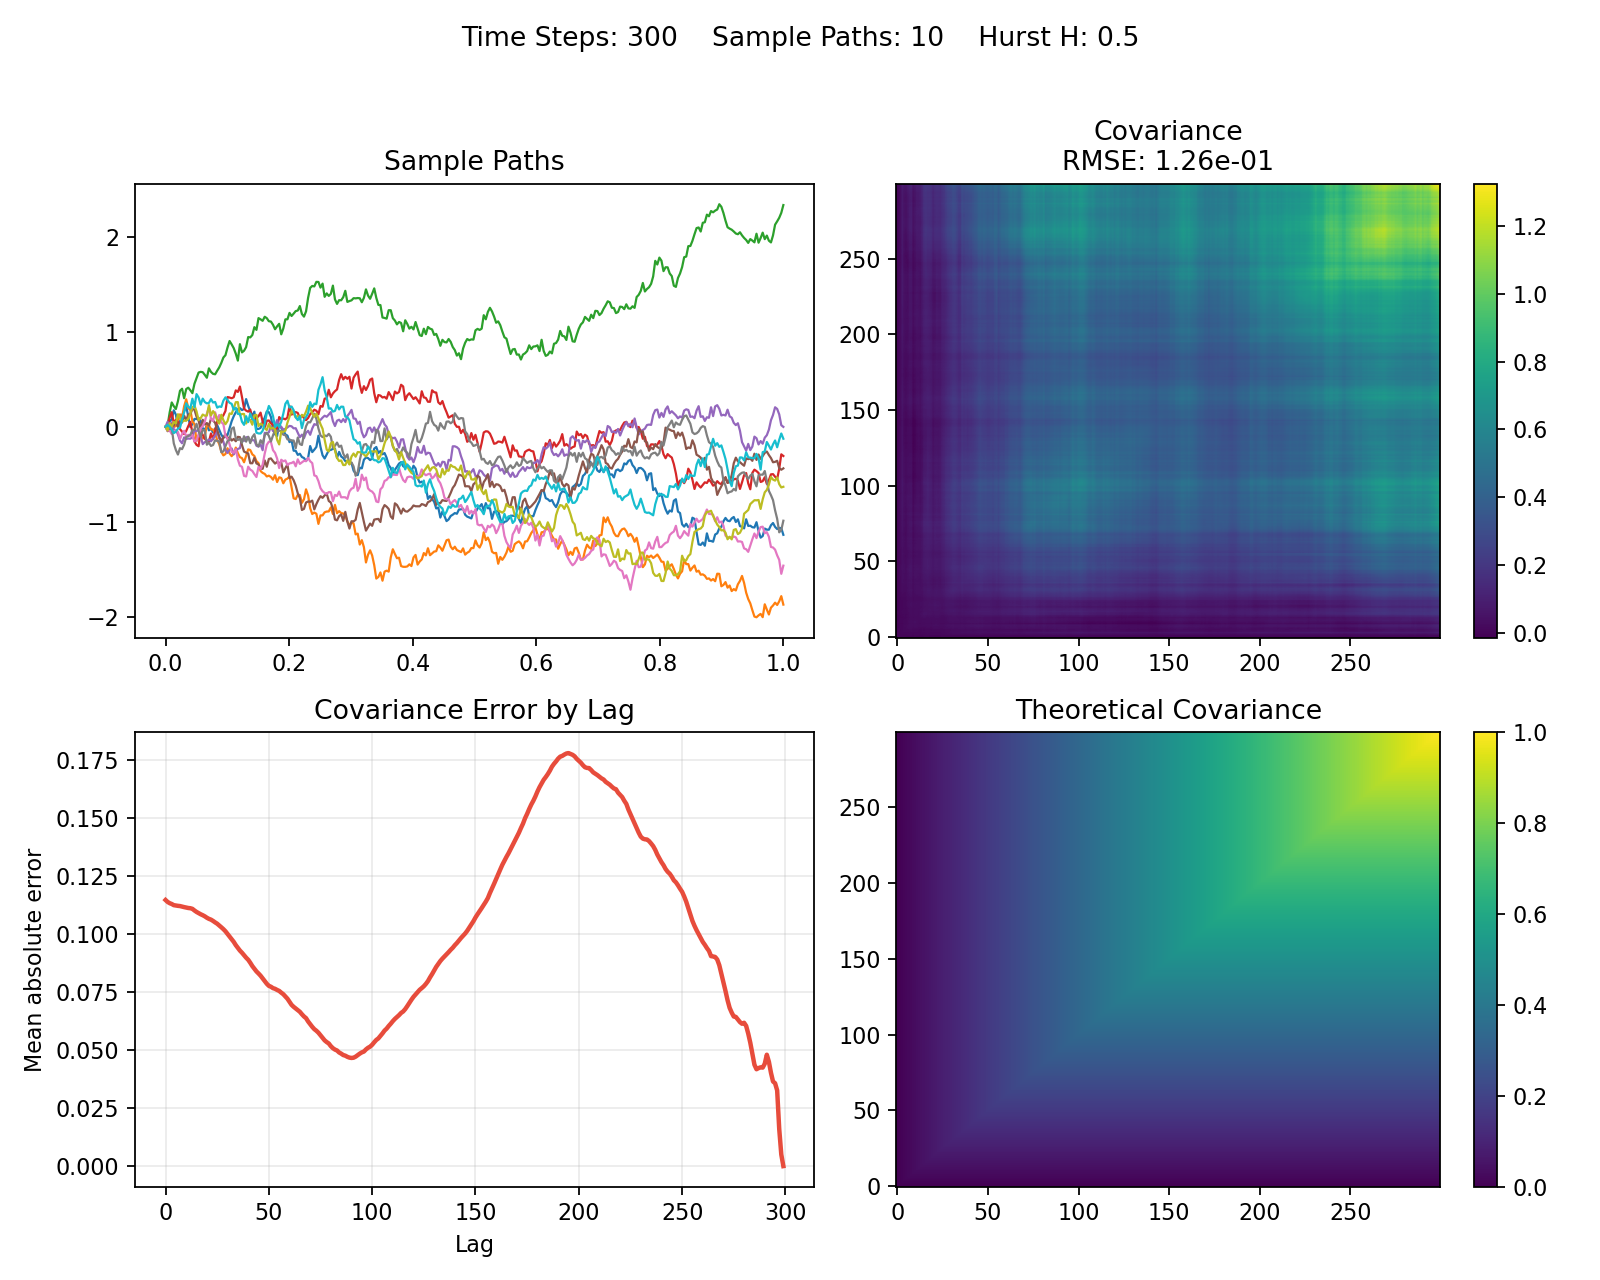
\includegraphics[width=\linewidth]{img/hft2-fgm0_5.png}
\end{minipage}

\vspace{1.2cm}

%==================== ROW 2 ====================
\begin{minipage}[c][0.24\textheight][c]{0.50\textwidth}
\centering
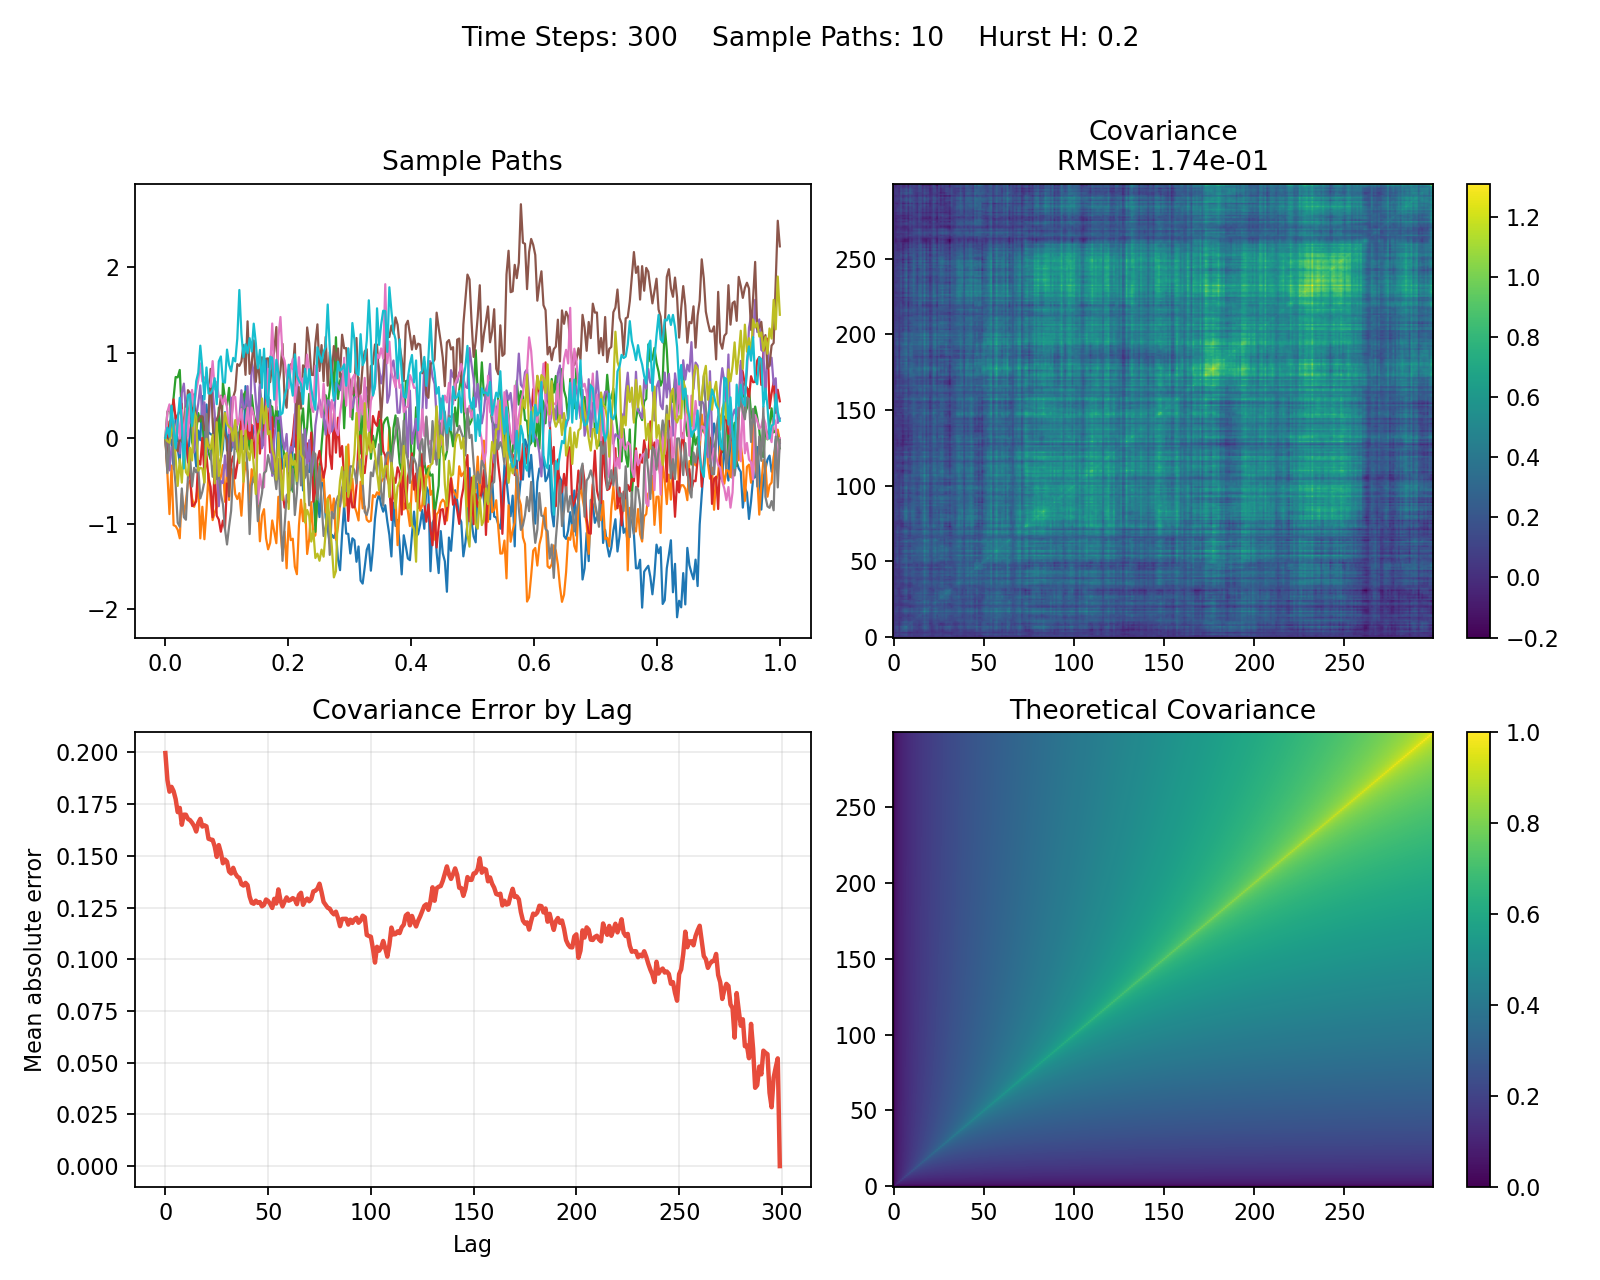
\includegraphics[width=\linewidth]{img/hft2-fgm0_2.png}
\end{minipage}
\hfill
\begin{minipage}[c][0.24\textheight][c]{0.44\textwidth}
\normalsize
\textbf{Anti-persistent regime: \(H=0.2\).}

\vspace{0.3em}

When \(H<\tfrac12\), successive increments tend to have opposite signs. This negative correlation creates a stronger tendency toward local reversals, so the paths appear rougher and more irregular. Compared with the benchmark case \(H=0.5\), the motion oscillates more frequently and displays less local trend continuation. This regime is especially useful when one wants to emphasize roughness and short-term alternation in the trajectory.
\end{minipage}

\vspace{0.8cm}

%==================== ROW 3 ====================
\begin{minipage}[c][0.24\textheight][c]{0.44\textwidth}
\normalsize
\vspace{0.5cm}

\textbf{Persistent regime: \(H=0.8\).}

\vspace{0.3em}

When \(H>\tfrac12\), increments become positively correlated. As a consequence, upward moves are more likely to be followed by upward moves, and downward moves by downward moves. The resulting paths look smoother and more persistent than in the Brownian benchmark. Long local excursions become more visible, and the sample paths exhibit a stronger sense of directional continuity.
\end{minipage}
\hfill
\begin{minipage}[c][0.24\textheight][c]{0.50\textwidth}
\centering
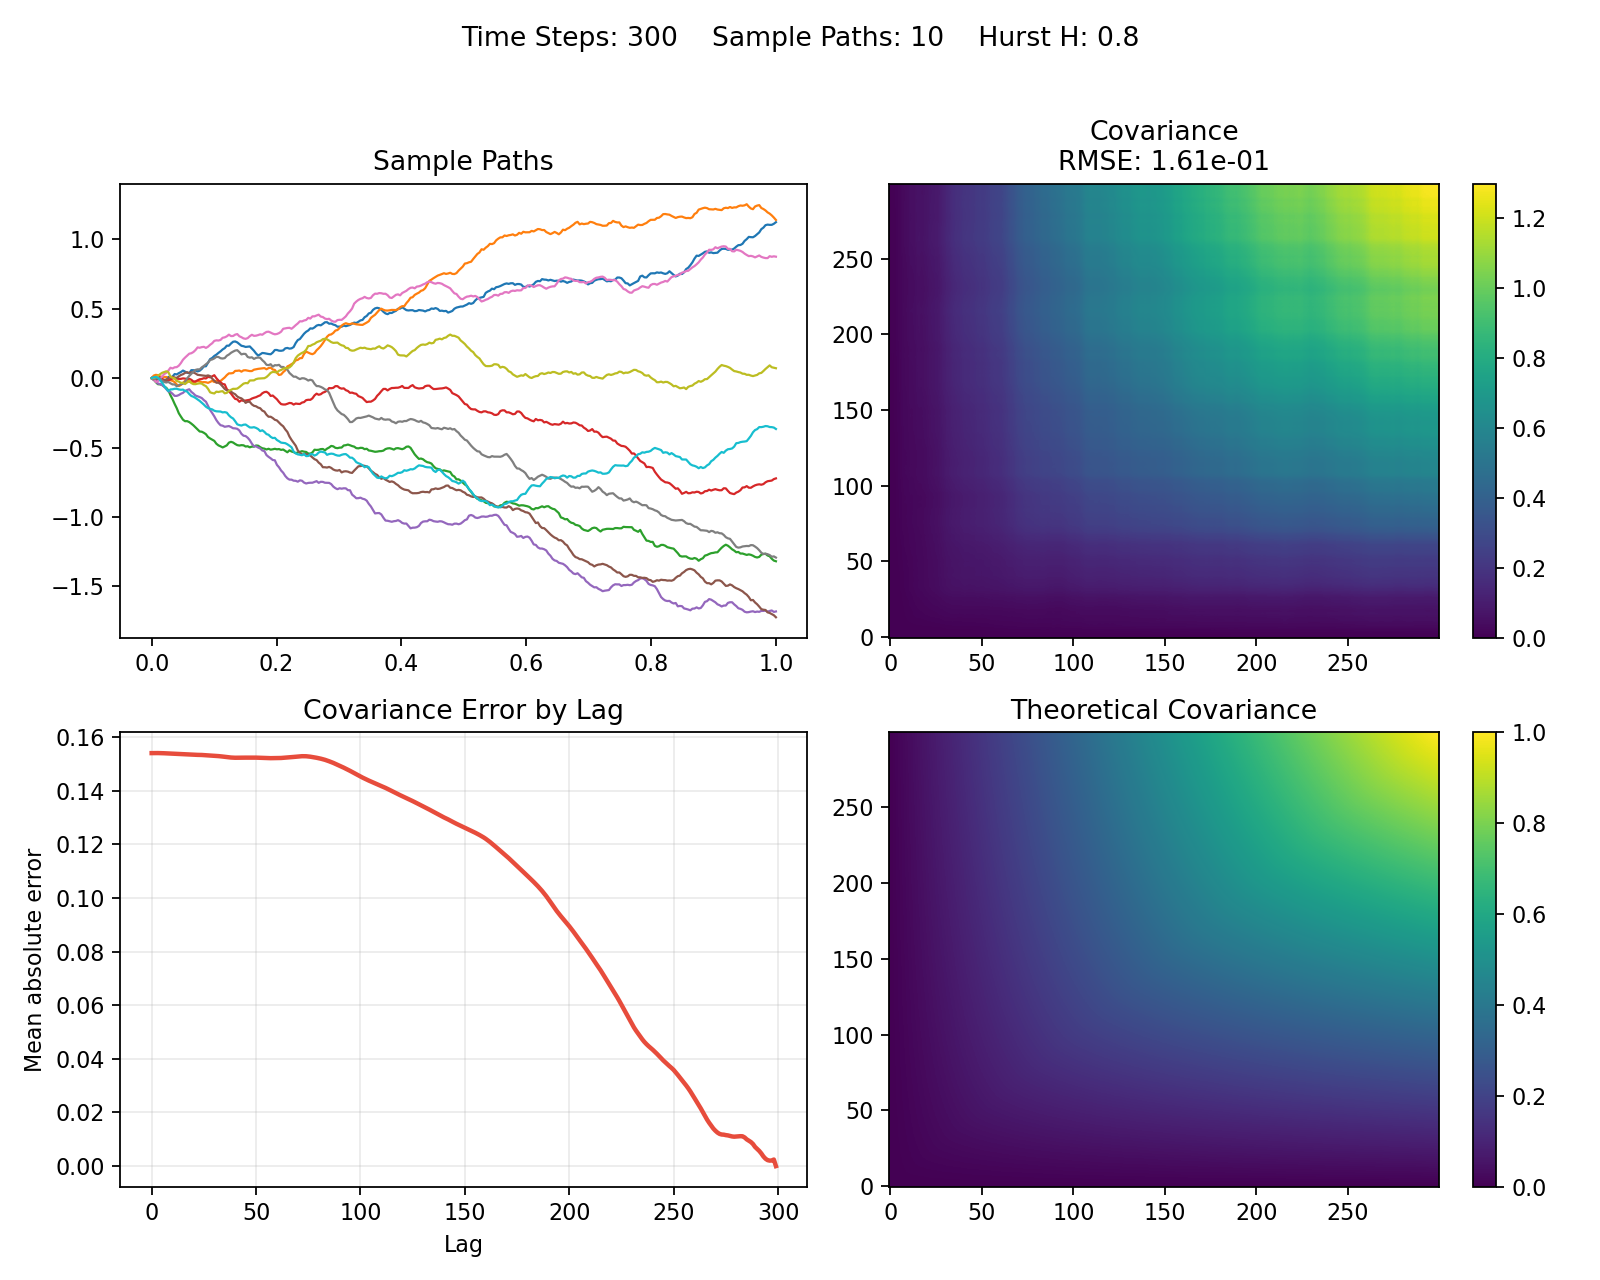
\includegraphics[width=\linewidth]{img/hft2-fgm0_8.png}
\end{minipage}

\end{figure}

\vspace{0.5cm}

\subsection{Financial applications and computational challenges}

The interest in fractional Brownian motion within quantitative finance is mainly motivated by its ability to encode temporal dependence beyond the Markovian paradigm. In particular, when volatility is modeled as a latent process rather than as a directly traded asset, long-memory or roughness effects can become empirically relevant. This is one of the reasons why fractional-type models, and especially rough-volatility specifications, have attracted growing attention in the literature.

A natural interpretation of this point arises through the dynamics of log-volatility. If volatility exhibits dependence across multiple time scales, then a path-dependent Gaussian driver may provide a richer description than standard Brownian motion. In rough-volatility applications, this motivates the use of non-Markovian Gaussian structures to capture irregular short-term behavior together with persistent dependence.

This additional realism, however, comes at a cost. Once volatility is driven by a non-Markovian process, the model no longer admits the simple low-dimensional state representation available in classical diffusion frameworks. As a consequence, pricing and calibration become substantially more expensive. If one wishes to fit such a model to an implied-volatility surface, the procedure typically requires repeated simulation of the full volatility path, followed by repeated pricing across a grid of strikes and maturities.

The difficulty is not limited to pricing alone. Calibration requires solving an inverse problem: one must search over a parameter space until the model-generated prices or implied volatilities match the observed surface. In a non-Markovian setting, each candidate parameter vector may require a full path simulation, making the overall procedure too costly for live or large-scale applications.

This trade-off has motivated a parallel line of research based on surrogate methods. Instead of rerunning the full pricing model at each calibration step, one can attempt to learn the map from model parameters to implied-volatility surfaces through neural networks or other machine-learning approximators. If successful, such a surrogate can dramatically accelerate calibration. At the same time, the gain in speed comes with its own issues: approximation error, limited extrapolation power, and the fact that desirable structural properties, such as no-arbitrage consistency, are not automatically guaranteed.

For this reason, fractional Brownian motion should be viewed not as a free improvement over standard models, but as a richer modeling choice that trades analytical tractability for empirical flexibility. This trade-off makes simulation methodology especially important. We therefore begin with the Davies--Harte construction, which is a convenient way to generate fractional Gaussian noise and fractional Brownian motion with the correct covariance structure.

\subsection{Davies--Harte Simulation and Validation}

The trajectories displayed in the visual comparison above are most naturally generated from the increment process rather than from a direct covariance factorization. Among the available simulation methods, the Davies--Harte scheme is particularly convenient because it is both mathematically transparent and computationally efficient: it generates fractional Gaussian noise by embedding its covariance sequence into a circulant structure diagonalized by the FFT, and then recovers fractional Brownian motion by cumulative summation.

\paragraph{Inputs.} The basic inputs of the scheme are
\[
H\in(0,1), \qquad T>0, \qquad N\in\mathbb{N},
\]
where \(H\) is the Hurst parameter, \(T\) is the terminal time, and \(N\) is the number of time steps. We also define
\[
\Delta t = \frac{T}{N},
\qquad
t_n = n\Delta t,
\qquad n=0,1,\dots,N.
\]
Increasing \(N\) refines time resolution. Agreement of empirical covariance with its theoretical target also depends on path count, validity of the embedding and sampling error; time-grid refinement alone does not guarantee closer empirical statistics.

\paragraph{Step 1: generate the time grid.} The first step is to discretize the interval \([0,T]\):
\[
t_n=n\Delta t,
\qquad n=0,1,\dots,N.
\]
This produces the \(N+1\) points on which the path will be represented.

\paragraph{Step 2: define the autocovariance of fractional Gaussian noise.} The Davies--Harte construction works directly with fractional Gaussian noise. Its autocovariance is
\[
\gamma_H(k)
=
\frac{1}{2}
\left(
|k+1|^{2H}
-
2|k|^{2H}
+
|k-1|^{2H}
\right),
\qquad k\in\mathbb{Z}.
\]
This formula determines the dependence structure of the increments and is the starting point of the whole algorithm.

\paragraph{Step 3: build the circulant covariance vector.} The key idea is to embed the covariance sequence into a circulant vector of length \(2N\). One convenient choice is
\[
c=
\bigl(
\gamma_H(0),\gamma_H(1),\dots,\gamma_H(N-1),0,
\gamma_H(N-1),\dots,\gamma_H(1)
\bigr).
\]
This step is crucial because circulant matrices are diagonalized by the discrete Fourier transform, which makes the method computationally efficient.

\paragraph{Step 4: compute the embedded eigenvalues via FFT.} Let
\[
m=2N.
\]
Applying the FFT to the circulant vector produces the embedded eigenvalues
\[
\lambda_j=\Re\bigl(\mathrm{FFT}(c)_j\bigr),
\qquad j=0,\dots,m-1.
\]
Since this is a covariance embedding, the relevant eigenvalues must be nonnegative up to numerical tolerance. In practice, one checks this explicitly before proceeding.

\paragraph{Step 5: generate the complex Gaussian vector.} The next step is to construct a complex Gaussian vector \(Z=(Z_0,\dots,Z_{m-1})\) with the conjugate symmetry required by the inverse transform. Let \(\xi_k,\eta_k\) be independent standard normal random variables. Then define
\[
Z_0=\sqrt{\lambda_0}\,\xi_0,
\qquad
Z_N=\sqrt{\lambda_N}\,\xi_N,
\]
and for \(k=1,\dots,N-1\),
\[
Z_k
=
\sqrt{\frac{\lambda_k}{2}}
\left(\xi_k+i\eta_k\right),
\qquad
Z_{m-k}=\overline{Z_k}.
\]
This is the most delicate part of the scheme. The conjugate assignment ensures that the inverse FFT will return a real-valued Gaussian sequence.

\paragraph{Step 6: apply the inverse FFT and restore the time scale.} Applying the inverse FFT to \(Z\) produces a realization of fractional Gaussian noise. However, one must be careful with scaling. In NumPy, the inverse FFT includes a factor \(1/m\), so a correction is needed. In addition, the correct time scale must be restored through \(\Delta t^H\). The simulated increments are therefore
\[
\Delta B_j^H
=
\Delta t^H\,\sqrt{m}\,
\Re\!\left(\mathrm{IFFT}(Z)_j\right),
\qquad j=0,\dots,N-1.
\]
The factor \(\sqrt{m}\) corrects the normalization introduced by the inverse FFT, while \(\Delta t^H\) ensures that
\[
\Var(\Delta B_j^H)=\Delta t^{2H}.
\]

\paragraph{Step 7: recover fractional Brownian motion by cumulative summation.} Once the increments have been generated, fractional Brownian motion is obtained by accumulation:
\[
B_0^H=0,
\qquad
B_{t_n}^H=\sum_{j=0}^{n-1}\Delta B_j^H,
\qquad n=1,\dots,N.
\]
This final step is conceptually simple but essential: the whole simulation procedure reduces to generating the correct correlated Gaussian increments and summing them.

\subsection{Simulation and confirmation against theoretical results}

Once the simulation scheme has been implemented, the next question is whether the output is actually correct. A plausible-looking path is not enough: even a small scaling mistake inside the FFT or inverse FFT can generate visually convincing trajectories whose empirical moments do not match the theoretical ones. For this reason, the simulation should be validated against the variance of fractional Gaussian noise, the variance of fractional Brownian motion, and the full covariance kernel of the process.

\paragraph{Variance of the increments and of the process.} The most immediate diagnostic consists in comparing empirical and theoretical variances. For the simulated fractional Gaussian noise, the theoretical variance is
\[
\Var(\Delta B_j^H)=\Delta t^{2H}.
\]
For fractional Brownian motion itself, the variance at time \(t_n\) is
\[
\Var(B_{t_n}^H)=t_n^{2H}.
\]
These two identities provide a simple but informative consistency check. The first confirms that the increment process has been scaled correctly, while the second confirms that the cumulative summation from fractional Gaussian noise to fractional Brownian motion has been implemented properly.

In practice, one generates many paths, computes empirical variances, and compares them to the theoretical targets. As the number of simulated paths and the grid resolution increase, the discrepancy should decrease.

\paragraph{Covariance-matrix confirmation.} A more informative validation compares the full empirical covariance matrix of the simulated process to the theoretical covariance kernel
\[
\Gamma_{ij}
=
\Cov(B_{t_i}^H,B_{t_j}^H)
=
\frac12\left(
t_i^{2H}+t_j^{2H}-|t_i-t_j|^{2H}
\right).
\]
Given \(M\) simulated paths \(B^{(1)},\dots,B^{(M)}\), one can estimate the empirical covariance matrix by
\[
\widehat{\Gamma}_{ij}
=
\frac{1}{M-1}
\sum_{r=1}^{M}
\left(B_{t_i}^{(r)}-\overline{B}_{t_i}\right)
\left(B_{t_j}^{(r)}-\overline{B}_{t_j}\right),
\]
where \(\overline{B}_{t_i}\) is the empirical mean at time \(t_i\). The discrepancy between empirical and theoretical covariance can then be summarized by the root mean squared error
\[
\mathrm{RMSE}
=
\left(
\frac{1}{(N+1)^2}
\sum_{i=0}^{N}\sum_{j=0}^{N}
\bigl(\widehat{\Gamma}_{ij}-\Gamma_{ij}\bigr)^2
\right)^{1/2}.
\]

This is the natural theoretical benchmark for the simulated paths shown earlier. The visual comparison in the previous figure illustrates how the geometry of the trajectories changes with \(H\); the covariance validation presented here explains why those paths are statistically consistent with the definition of the process.

\paragraph{Error decay in \(N\) and \(M\).} A correct implementation should not only reproduce the covariance structure at one fixed parameter choice, but should also exhibit the expected improvement as the numerical inputs increase. There are two natural directions along which to check this.

First, increasing \(N\) refines the time grid and improves the empirical representation of the increment process. In particular, one may study how the RMSE associated with the variance of fractional Gaussian noise decreases as the grid becomes finer.

Second, increasing the number of simulated paths \(M\) improves the empirical estimation of the covariance matrix. Since covariance estimation is a Monte Carlo object, the RMSE should decay at the standard rate
\[
\mathrm{RMSE}=O(M^{-1/2}).
\]
This provides a useful benchmark: if the implementation is correct, increasing the sample size should reduce the covariance estimation error approximately at that rate.


\begin{algorithm}[H]
\caption{Validation diagnostics before the convergence figure}
\DontPrintSemicolon
\For{each grid size \(N\)}{
  simulate fractional Gaussian noise and compare empirical increment variance with \(\Delta t^{2H}\)\;
}
\For{each number of paths \(M\)}{
  estimate the empirical covariance matrix of \(B^H\)\;
  compare it with the theoretical covariance kernel and record the RMSE\;
}
plot both error curves against their theoretical decay benchmarks\;
\end{algorithm}

\begin{figure}[H]
\centering
\begin{minipage}[t]{0.48\textwidth}
\centering
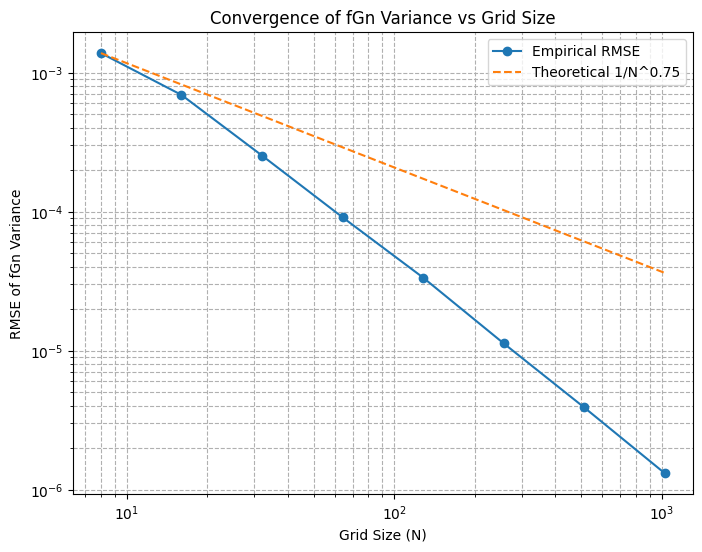
\includegraphics[width=\linewidth]{img/hft2-img_4.png}
\end{minipage}
\hfill
\begin{minipage}[t]{0.48\textwidth}
\centering
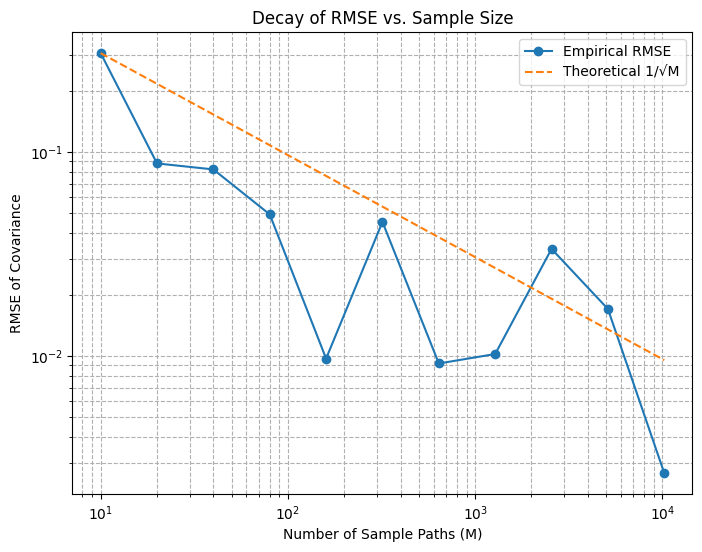
\includegraphics[width=\linewidth]{img/hft2-img_5.png}
\end{minipage}
\caption{Convergence diagnostics for the Davies--Harte implementation. The left panel compares the empirical decay of the RMSE for the variance of fractional Gaussian noise with the theoretical benchmark as the grid size \(N\) increases. The right panel compares the empirical decay of the covariance RMSE with the Monte Carlo reference rate \(1/\sqrt{M}\) as the number of simulated paths \(M\) grows.}
\label{hft2-fig:fbm_convergence_diagnostics}
\end{figure}

Taken together, these checks provide a coherent validation strategy. First, one verifies that the increment process and the accumulated process have the correct variance scaling. Then, one compares the full empirical covariance matrix to the theoretical covariance kernel. Finally, one checks that the numerical error decreases in the expected way as \(N\) and \(M\) increase. Figure \ref{hft2-fig:fbm_convergence_diagnostics} illustrates these convergence patterns directly. The decay in the left panel is consistent with improved variance accuracy on finer grids, while the right panel shows the expected overall reduction in covariance error as the sample size increases, despite the visible finite-sample noise typical of Monte Carlo experiments.

\subsection{Problems of Davies--Harte simulations}

The Davies--Harte scheme is an elegant and efficient way to generate fractional Gaussian noise and, by cumulative summation, fractional Brownian motion. For offline Monte Carlo experiments it is extremely useful, since it reproduces the target covariance structure accurately and does so at relatively low computational cost. For the purposes of this study, however, this efficiency comes with an important limitation: the construction is fundamentally global rather than causal.

The issue is not that fractional Brownian motion itself depends on future information. It does not. The issue is instead numerical and structural. In the Davies--Harte scheme, one fixes the entire time grid in advance, embeds the covariance sequence into a circulant structure, applies spectral methods, and generates the full trajectory at once. In this sense, the algorithm requires \emph{global path knowledge}: the desired covariance structure is enforced through a construction that acts on the whole path simultaneously, rather than through a recursive state update based only on past shocks.

This point matters in sequential financial applications. In market making, filtering, and related control problems, one typically wants a representation that evolves forward in time as new information arrives. At each time \(t\), the state should be updated causally from what is already known, without relying on a simulation architecture that is tied to the full terminal horizon. From this perspective, Davies--Harte is mathematically valid and computationally efficient, but it is not the most natural language for an online control problem.

A related limitation appears in model fitting. If one were to use a non-Markovian volatility specification driven by fractional Brownian motion and calibrate it to an implied-volatility surface, then in the absence of a closed-form pricing formula one would typically need repeated Monte Carlo simulation. For each parameter choice, one must simulate the full volatility path, generate prices over a grid of strikes and maturities, compare the model output with the observed surface, and then iterate over the parameter space. Even if the underlying simulator is efficient, this overall calibration loop quickly becomes computationally intensive and may become impractical in a live setting.

There is therefore a genuine trade-off. On the one hand, rough or long-memory dynamics may capture empirically relevant dependence structures more faithfully than classical Markovian diffusions. On the other hand, these gains do not come for free: they are purchased with greater numerical cost and with the loss of a simple recursive state representation. In particular, while Davies--Harte is well suited for global path generation and covariance-based validation, it is not the most convenient framework when the final objective is a causal simulation architecture for sequential pricing or inventory control.

For these reasons, the Davies--Harte scheme should be regarded as an excellent benchmark for simulation and validation, but not yet as the most natural representation for control-oriented modeling. What is needed next is a formulation that preserves memory while making causality explicit. This is precisely the role of Gaussian Volterra processes: they replace the global covariance viewpoint with a kernel-based construction in which the state at time \(t\) depends on past noise only. This makes them a more natural starting point for rough-volatility simulation, approximation, and eventually market-making control.

%%%%%%%%%%%%%%%%%%%%%%%%%%%%%%%%%%%%%%%%%%%%%%%%
%%%%%%%%%%%%%%%%%%%%%%%%%%%%%%%%%%%%%%%%%%%%%%%%
%%%%%%%%%%%%%%%%%%%%%%%%%%%%%%%%%%%%%%%%%%%%%%%%

\section{Volterra Gaussian Processes and Causality}


\paragraph{From global covariance to causal kernels.}

Given a Brownian driver, the Volterra kernel assigns a weight to every shock that is already observable at time \(t\). This separates two roles that a covariance-first simulator leaves implicit: the support condition determines which shocks may enter the state, while the kernel profile determines their relative influence. That distinction is useful in a pricing engine or control loop because it exposes the information set used by each update.

This is the main difference with covariance-based simulation methods such as Davies--Harte. There, the objective is to sample the entire path with the correct law, and this is done through a global embedding of the covariance sequence. In a Volterra representation, by contrast, one builds the process forward in time through a weighted accumulation of Brownian shocks. The weights are determined by the kernel, and therefore the kernel becomes the object that controls both the dependence structure and the geometry of the paths.

\subsection{General Volterra representation}

\begin{definition}[Gaussian Volterra process]
Let \(W\) be a standard Brownian motion and let \(K(t,s)\) be a measurable kernel such that
\(
K(t,s)=0 \; \text{for } s>t,
\; \text{and}  \;
\int_0^t K(t,s)^2\,ds<\infty
\; \text{for all } t\ge 0.
\)
A \emph{Gaussian Volterra process} is a process of the form
\[
X_t=\int_0^t K(t,s)\,dW_s.
\]
\end{definition}

The condition \(K(t,s)=0\) for \(s>t\) is the mathematical expression of causality: the process at time \(t\) depends only on shocks observed before time \(t\). The entire covariance structure is therefore encoded in the kernel itself.

\subsection{Covariance induced by the kernel}

The key step is to show how the kernel determines the covariance of the process. Since the stochastic integral is centered, one expects the covariance to reduce to an expectation of a product of integrals, which can then be simplified by It\^o isometry.

\begin{proposition}[Covariance induced by a Volterra kernel]
Let
\[
X_t=\int_0^t K(t,s)\,dW_s.
\]
Then for any \(s,t\ge 0\),
\[
\Cov(X_s,X_t)
=
\int_0^{s\wedge t} K(s,u)K(t,u)\,du.
\]
\end{proposition}

\begin{proof}
Since \(X_s\) and \(X_t\) are centered Gaussian variables,
\[
\Cov(X_s,X_t)=\E[X_sX_t].
\]
Using the stochastic integral representation,
\[
\E[X_sX_t]
=
\E\!\left[
\left(\int_0^s K(s,u)\,dW_u\right)
\left(\int_0^t K(t,v)\,dW_v\right)
\right].
\]
By It\^o isometry for products of stochastic integrals,
\[
\E\!\left[
\left(\int_0^s f(u)\,dW_u\right)
\left(\int_0^t g(v)\,dW_v\right)
\right]
=
\int_0^{s\wedge t} f(u)g(u)\,du.
\]
Applying this with \(f(u)=K(s,u)\) and \(g(u)=K(t,u)\) gives
\[
\Cov(X_s,X_t)
=
\int_0^{s\wedge t} K(s,u)K(t,u)\,du. \qedhere
\]
\end{proof}
    
This identity is the central bridge between the process and its second-order structure. It shows that once the kernel is selected, the covariance is no longer imposed externally: it is generated mechanically by the causal accumulation of Brownian shocks.

\paragraph{Why causality matters.}

The formula above also explains why the upper integration limit becomes \(s\wedge t\). If \(u>s\), then \(K(s,u)=0\) by causality; similarly, if \(u>t\), then \(K(t,u)=0\). Hence the product \(K(s,u)K(t,u)\) can only be nonzero when \(u\le s\) and \(u\le t\), which is equivalent to \(u\le s\wedge t\).

This point is important in sequential financial applications. In an online control problem one does not want a representation that is tied to the whole terminal horizon or to a global covariance embedding. Instead, one wants a state variable that can be updated as new information arrives. A Volterra process has exactly this interpretation: it is built from past noise only, with the memory of the process encoded through the kernel.

At the same time, causality should not be confused with Markovianity. A causal Volterra process may still be strongly non-Markovian. The value at time \(t\) does not depend on future noise, but it may depend on the entire past history of the driving Brownian motion. This is precisely what makes Volterra processes flexible enough to reproduce both rough and persistent behavior.

\subsection{Discretization and non-Markovian structure}

Once the Volterra representation is available, discretization is conceptually simple. Fix a horizon \(T>0\) and choose a uniform grid
\(
0=t_0<t_1<\cdots<t_n=T,
\quad
t_i=\frac{iT}{n},
\quad
\Delta t=\frac{T}{n}.
\)
Let
\[
\Delta W_j = W_{t_{j+1}}-W_{t_j},
\quad
\Delta W_j\sim \mathcal{N}(0,\Delta t),
\]
with independent increments across \(j\). A Riemann--It\^o approximation of the stochastic integral then yields
\[
X_{t_i}
\approx
\sum_{j=0}^{i-1} K(t_i,t_j)\,\Delta W_j.
\]

This discrete expression is the natural simulation recipe: choose a kernel, generate Brownian increments, and at each time point accumulate the past shocks with the appropriate weights. After the grid values have been obtained, one may visualize the path through piecewise linear interpolation, which is simply the numerical analogue of joining the dots.

\paragraph{Iterative construction.}

The discretized Volterra process can be built step by step from left to right. At the first nonzero grid point,
\[
X_{t_1}\approx K(t_1,t_0)\,\Delta W_0.
\]
At the next step,
\[
X_{t_2}\approx K(t_2,t_0)\,\Delta W_0 + K(t_2,t_1)\,\Delta W_1,
\]
and more generally
\[
X_{t_i}\approx \sum_{j=0}^{i-1} K(t_i,t_j)\,\Delta W_j.
\]

This already makes the causal structure visible: to build \(X_{t_i}\), one needs only the Brownian increments observed before time \(t_i\). But the same formula also shows why the process is non-Markovian in general. Indeed, the increment from \(t_{i-1}\) to \(t_i\) is
\[
X_{t_i}-X_{t_{i-1}}
\approx
K(t_i,t_{i-1})\,\Delta W_{i-1}
+
\sum_{j=0}^{i-2}
\bigl(K(t_i,t_j)-K(t_{i-1},t_j)\bigr)\,\Delta W_j.
\]
Unless the kernel is trivial, the new increment depends not only on the most recent shock, but also on the entire path history through all previous \(\Delta W_j\). This is exactly the discrete manifestation of non-Markovianity.

The special case in which this dependence disappears is standard Brownian motion. If one chooses the trivial kernel
\(
K(t,s)=1,
\; 0\le s<t,
\)
then
\[
X_t=\int_0^t dW_s = W_t,
\]
and the increment structure collapses to the familiar Markovian setting. This observation is useful: the Volterra framework contains Brownian motion as a limiting benchmark, but becomes genuinely non-Markovian as soon as the kernel introduces memory.
\subsection{Representative kernels and induced dynamics}

The flexibility of the Volterra representation comes from the choice of kernel. Different kernels induce different covariance structures and therefore different path dynamics.

\textbf{Brownian kernel}

The simplest example is
\(
K_{\mathrm{BM}}(t,s)=1.
\)
This reproduces standard Brownian motion,
\[
X_t=\int_0^t dW_s=W_t.
\]
In this case the Volterra construction is mathematically correct but computationally unnecessary, since Brownian motion can be simulated directly from independent Gaussian increments. Its main value here is conceptual: it shows that a Markovian process is contained as a special case in the broader Volterra family.

\textbf{Exponential kernel and mean reversion}

A second important example is the exponential kernel
\[
K_{\theta}(t,s)=e^{-\theta(t-s)}\mathbf{1}_{\{0\le s<t\}},
\qquad \theta>0.
\]
This kernel generates the Ornstein--Uhlenbeck process
\[
X_t=\int_0^t e^{-\theta(t-s)}\,dW_s,
\]
which solves the mean-reverting stochastic differential equation
\[
dX_t=-\theta X_t\,dt + dW_t.
\]
The exponential decay gives more weight to recent shocks than to distant ones, producing the familiar pull back toward the mean.

\textbf{Fractional-type kernel and roughness}

The rough-volatility literature is driven by singular power-law kernels. A simple causal prototype is
\[
\widetilde{K}_H(t,s)
=
\sqrt{c_H}\,(t-s)^{H-\frac12}\mathbf{1}_{\{0\le s<t\}},
\qquad
c_H=\frac{\Gamma(2H+1)}{2\,\Gamma(H+\frac12)^2},
\]
with \(H\in(0,1)\). The kernel is singular near the diagonal \(t=s\), which means that very recent history receives a particularly large weight. This is what generates roughness when \(H<\tfrac12\) and smoother, more persistent behavior when \(H>\tfrac12\). In the diagnostic implementation, the boundary value \(H=\tfrac12\) is treated separately with the exact Brownian kernel \(K(t,s)=\mathbf{1}_{\{s<t\}}\), so the resulting process is standard Brownian motion rather than the limiting normalization of this prototype.

\begin{remark}[Exact versus simplified fractional kernels]
Standard fractional Brownian motion admits an exact Volterra representation with a kernel \(K_H(t,s)\), but the closed form is more involved than a simple power law. In numerical intuition and in many rough-volatility approximations, one instead works with a tractable causal power-law kernel whose local behavior reproduces the desired roughness exponent. This chapter follows that practical route, since the goal is to prepare a simulation architecture rather than a complete classification of exact Gaussian representations.
\end{remark}

\subsection{Visual comparison across Hurst parameters}

The effect of the kernel is easiest to understand visually. In the panels below, the left block for each value of \(H\) illustrates the iterative construction of the process through a filtration window: as the window expands, the path is built using progressively more past information, exactly as required by causality. The right block shows the corresponding Volterra diagnostics, including sample paths, the kernel heat map, the Brownian driver, the full support of representative kernel slices, and the covariance induced by the discrete kernel. The reported RMSE compares that induced covariance with the standard fractional-Brownian target; it is zero up to numerical precision in the Brownian benchmark and need not vanish for the simplified power-law kernels.

\begin{algorithm}[H]
\caption{Reading the Volterra construction panels}
\DontPrintSemicolon
choose a causal kernel \(K_H(t,s)\) and Brownian increments \(\Delta W_j\)\;
\For{each time index \(i\)}{
  compute \(X_{t_i}\approx\sum_{j<i}K_H(t_i,t_j)\Delta W_j\) using past shocks only\;
  reveal the filtration window that is available at that step\;
}
plot the iterative path construction beside the kernel, noise, causality, and covariance diagnostics\;
\end{algorithm}



\begin{figure}[H]
\vspace{0cm}
\centering
\begin{minipage}[t]{0.44\textwidth}
\vspace{0cm}
\normalsize


\textbf{Benchmark regime: \(H=0.5\).}

The value \(H=\tfrac12\) is the exact Brownian benchmark. Here \(K(t,s)=1\) for \(s<t\) and \(K(t,s)=0\) for \(s\ge t\), so each kernel slice is flat over the observed past and drops to zero over the future. Consequently \(X_t=\int_0^t dW_s=W_t\): disjoint increments are independent and there is no fractional memory, although the construction remains causal because no future shock enters the state. The kernel heat map and the covariance heat map use the same numerical color range \([0,1]\), but their shapes differ by construction: the first is the binary support kernel, while the second is \(\Cov(W_t,W_s)=\min(t,s)\).

\vspace{0.5cm}
\centering
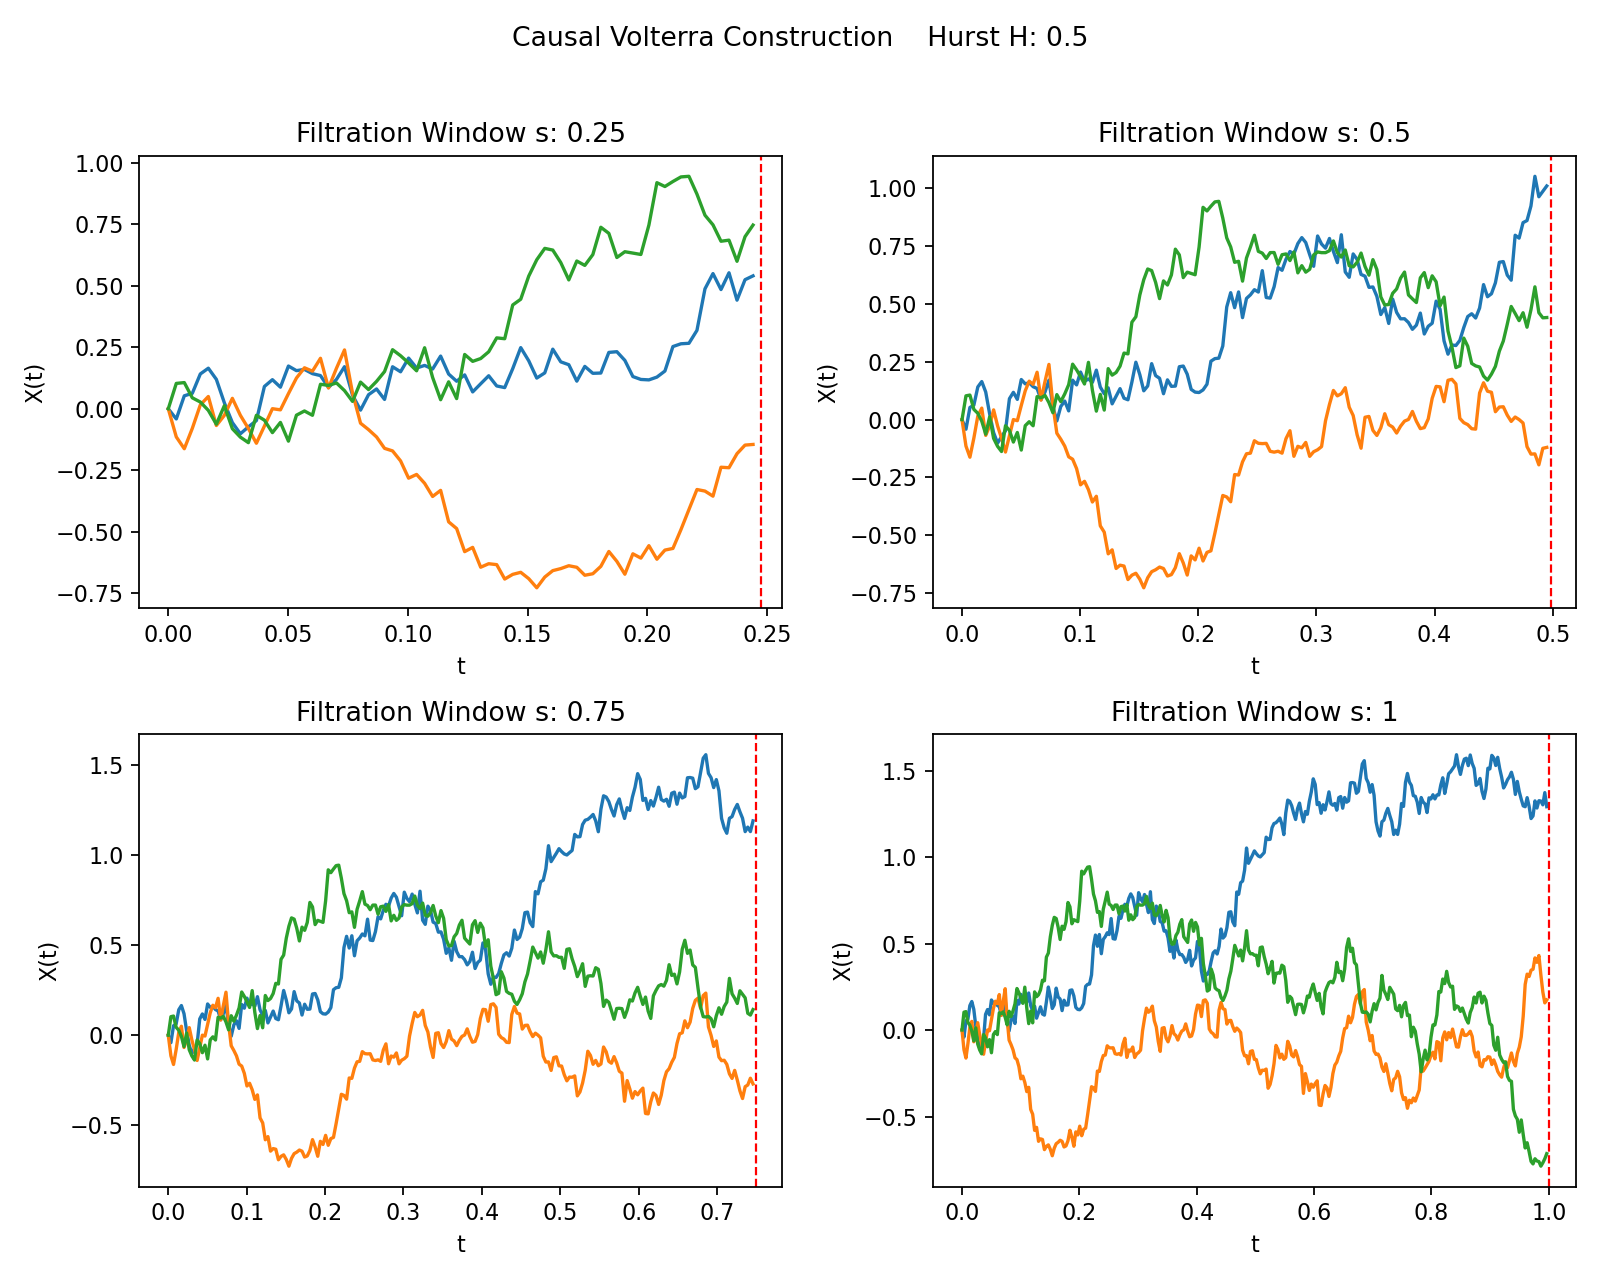
\includegraphics[width=\linewidth]{img/hft2-iterative0_5.png}
\end{minipage}
\hfill
\begin{minipage}[t]{0.54\textwidth}
\vspace{0.2cm}
\centering
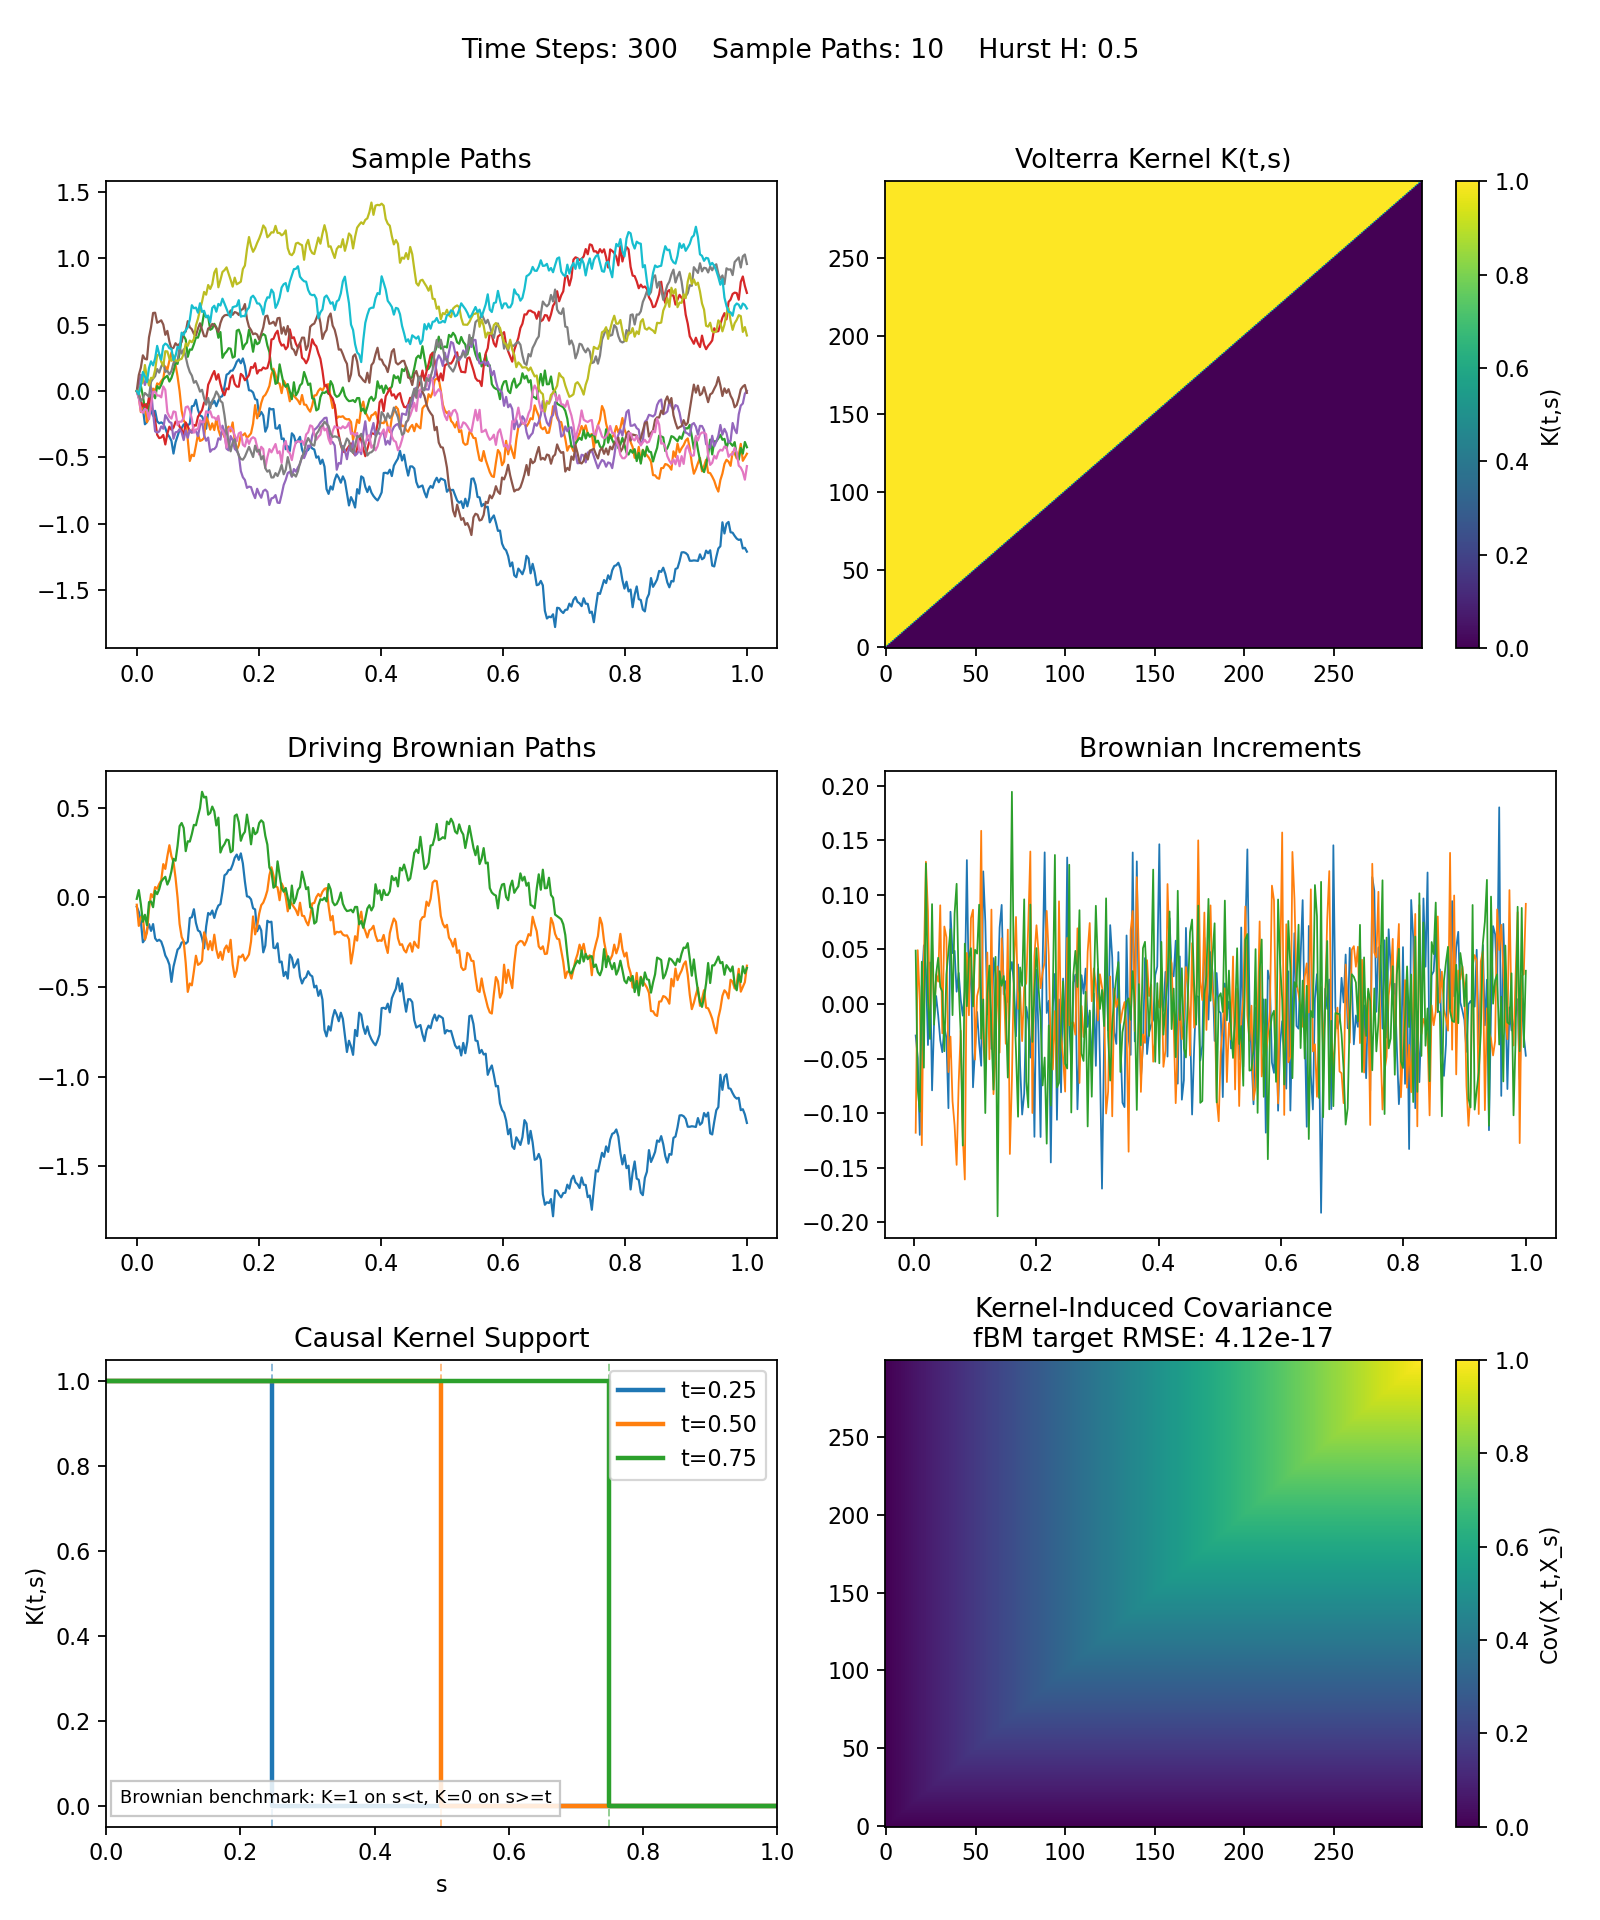
\includegraphics[width=\linewidth]{img/hft2-volterra0_5.png}
\end{minipage}
\end{figure}


\begin{figure}[H]
\centering
\begin{minipage}[t]{0.44\textwidth}
\vspace{0pt}
\normalsize
\textbf{Rough regime: \(H=0.2\).}

When the Hurst parameter is below $\tfrac12$ , the fractional-type kernel becomes more singular near the diagonal. This means that the process places a very large weight on the most recent shocks, while still retaining memory of the older ones. The iterative panels make this point visible: as the filtration window increases, the process is updated only from the observed past, but the contribution of the most recent increments remains dominant. 
This produces irregular, rapidly oscillating paths. 
Because the displayed power-law kernel is a tractable fractional-type prototype rather than the exact fractional-Brownian kernel, 
the covariance panel reports its 
discrepancy from the exact 
%fBM target instead of asserting equality.

\vspace{0pt}
\centering
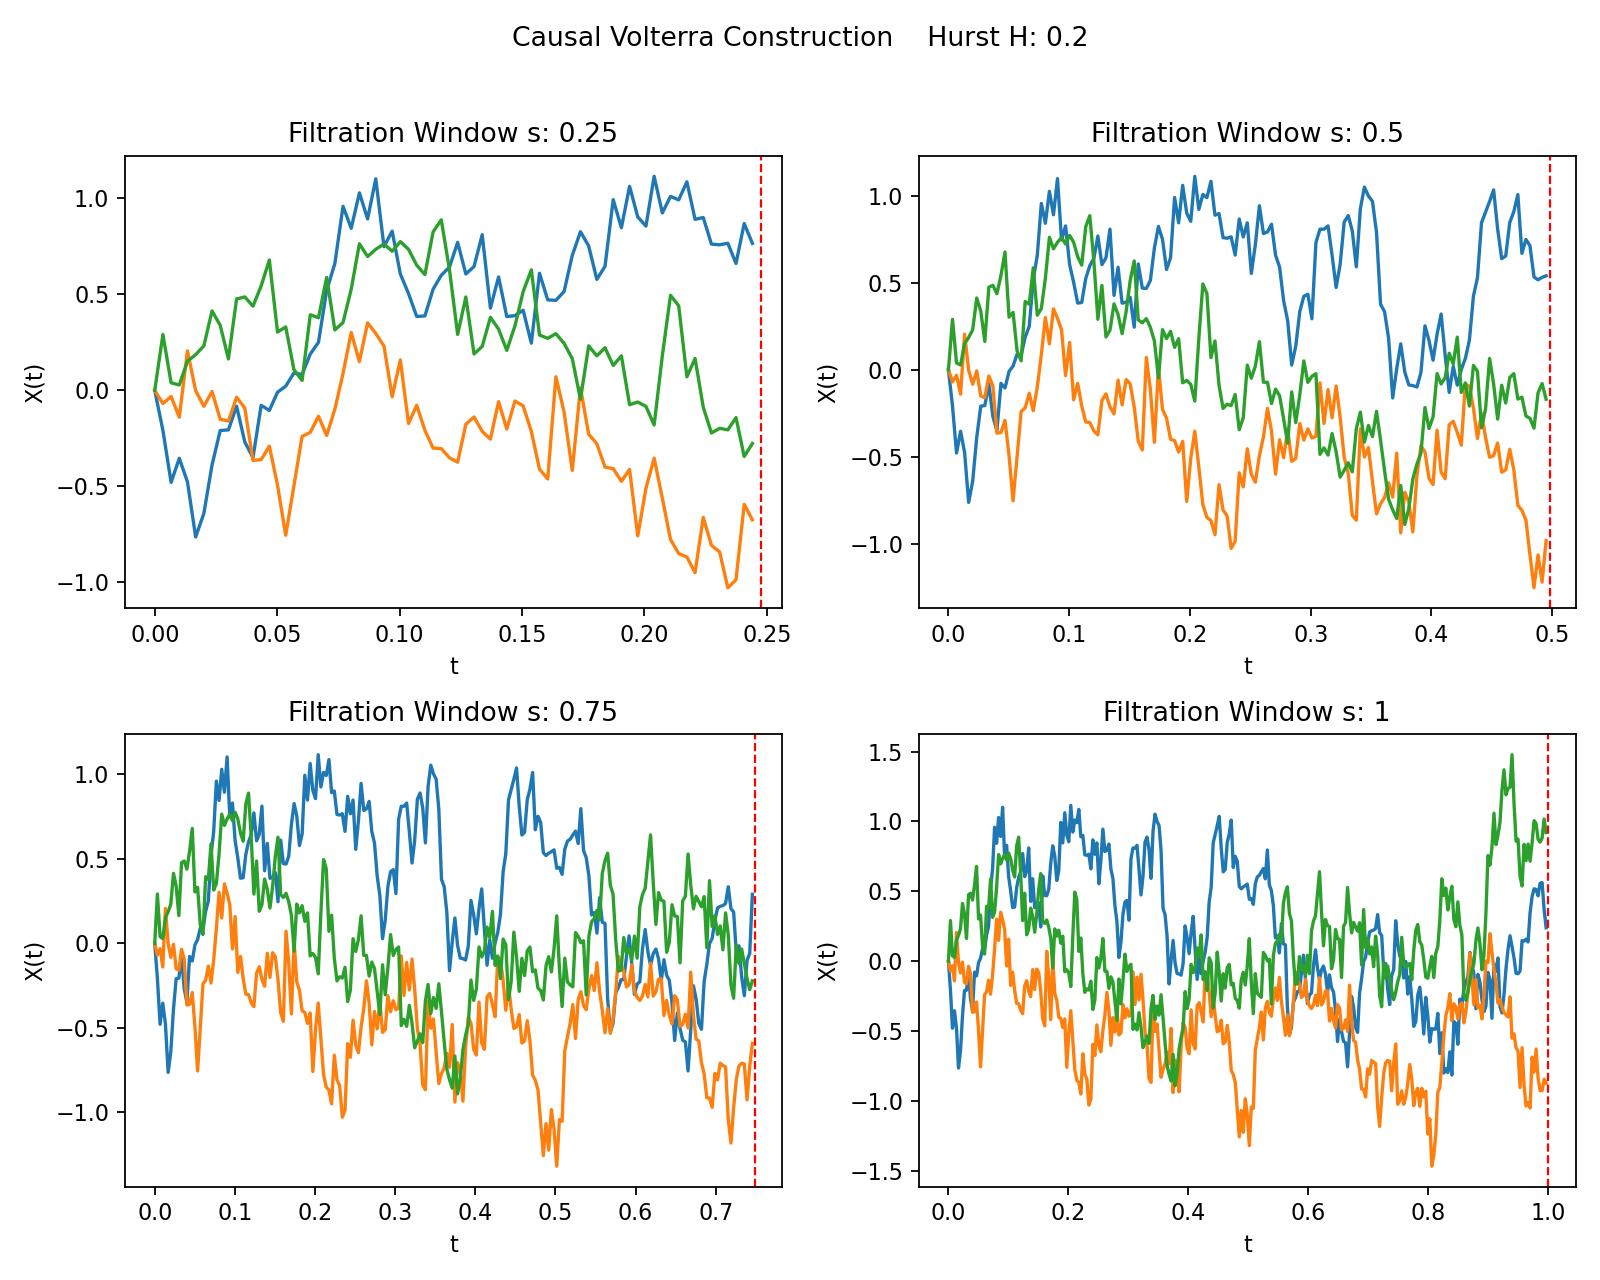
\includegraphics[width=\linewidth]{img/hft2-iterative0_2.png}
\end{minipage}
\hfill
\begin{minipage}[t]{0.52\textwidth}
\vspace{0pt}
\centering
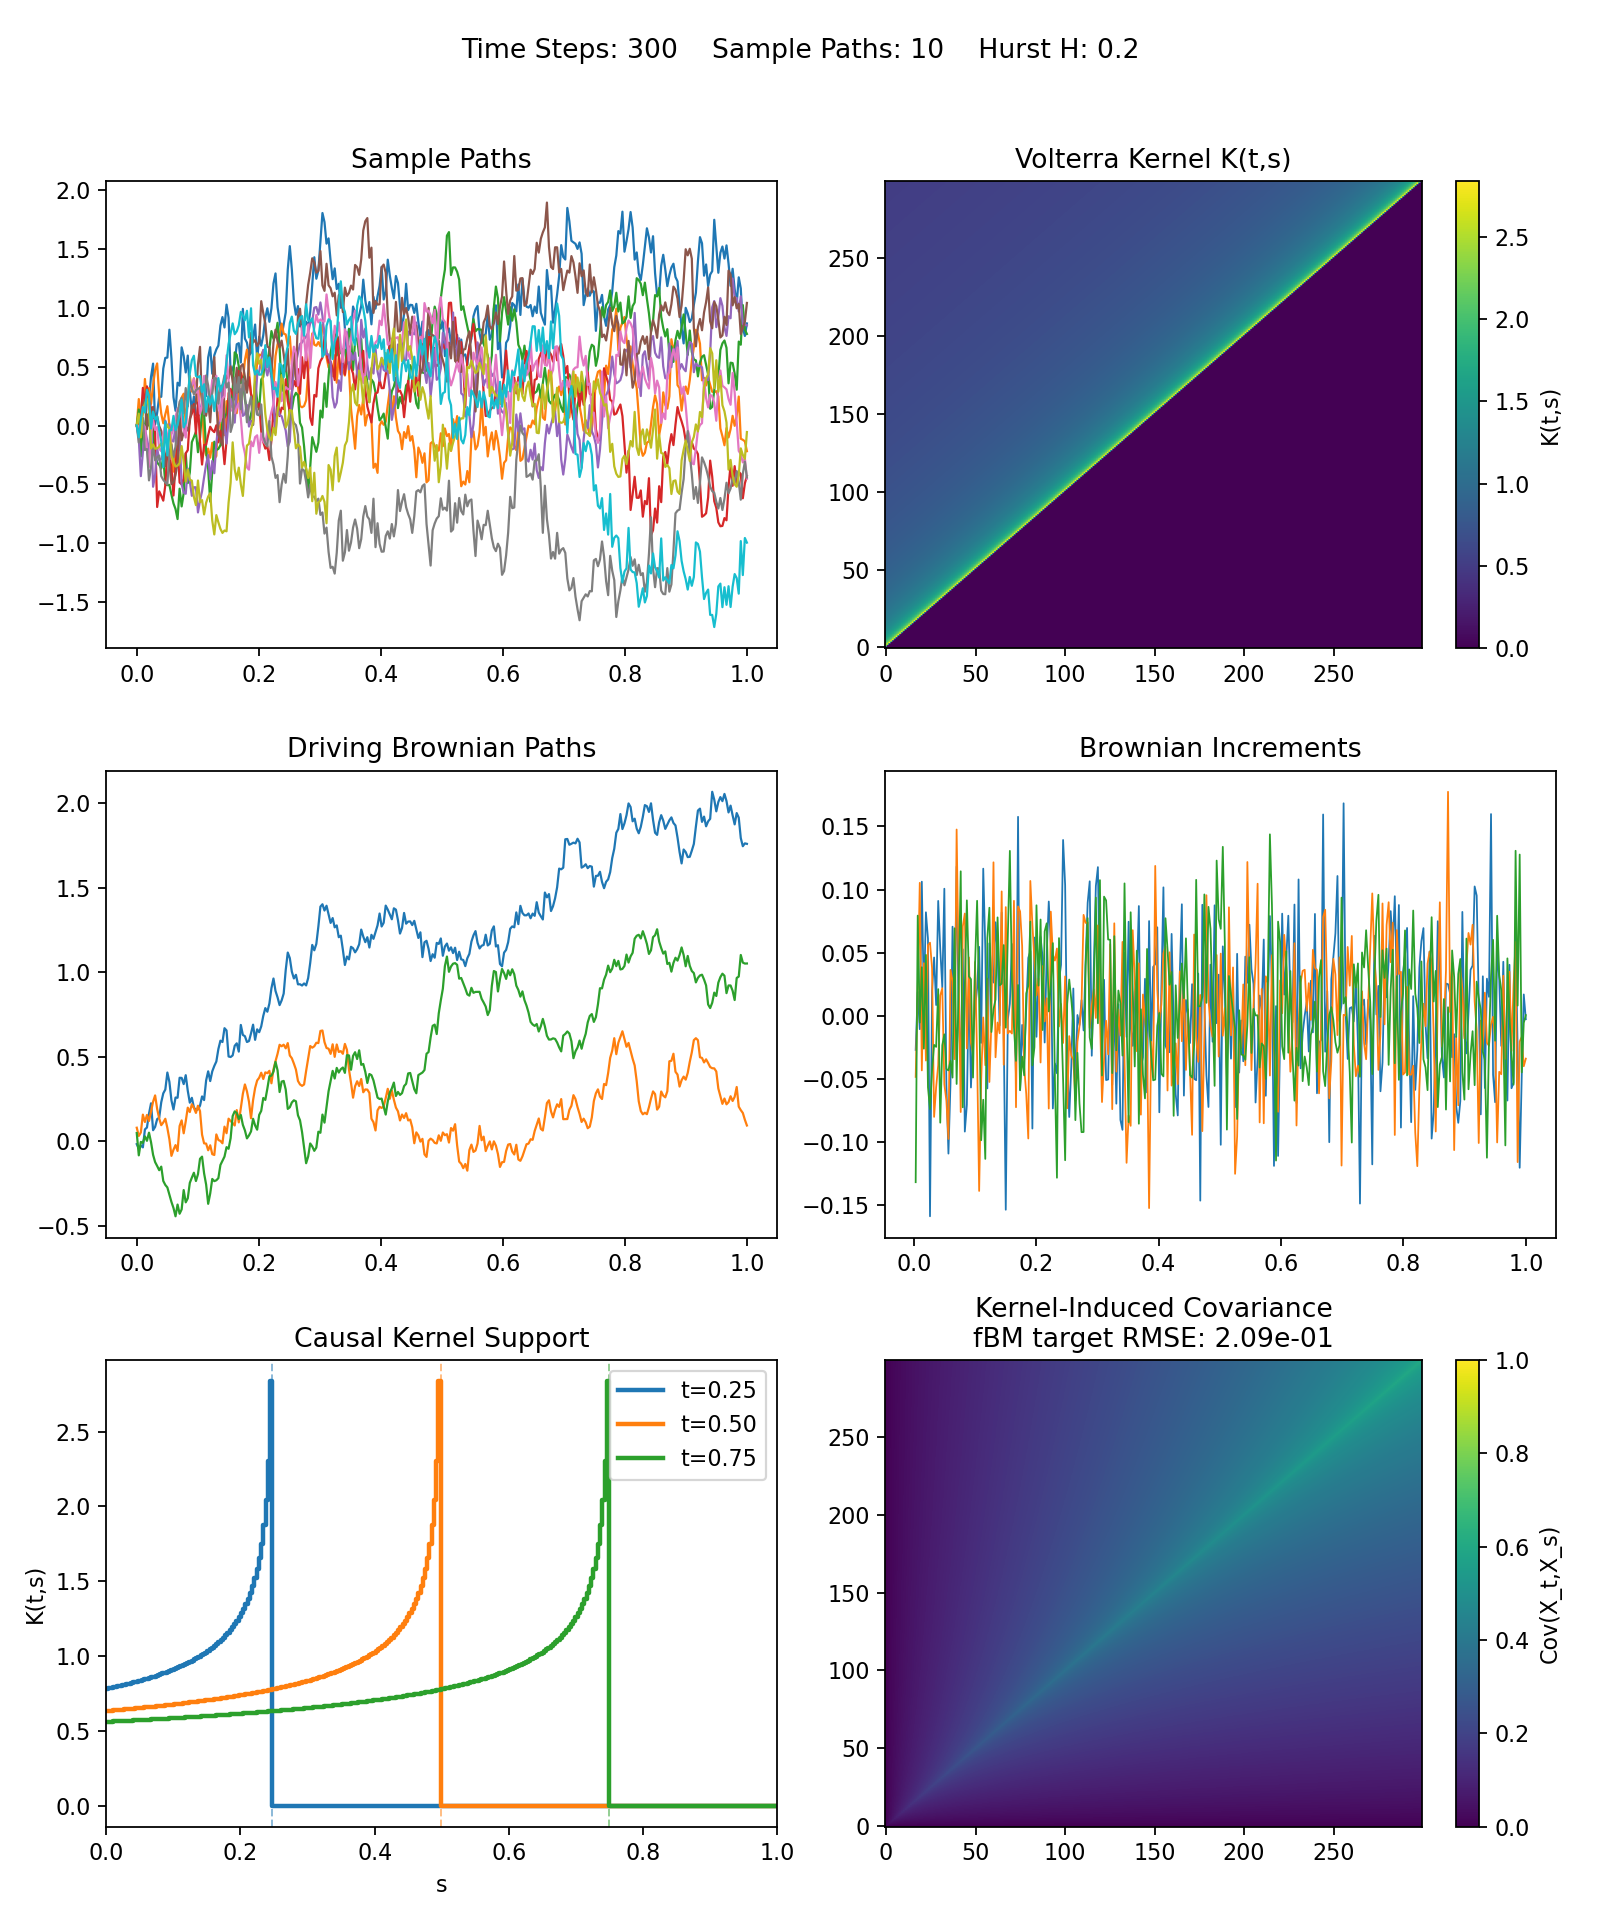
\includegraphics[width=\linewidth]{img/hft2-volterra0_2.png}
\end{minipage}
\end{figure}

\begin{figure}[H]
\centering
\begin{minipage}[t]{0.52\textwidth}
\vspace{0.4cm}
\centering
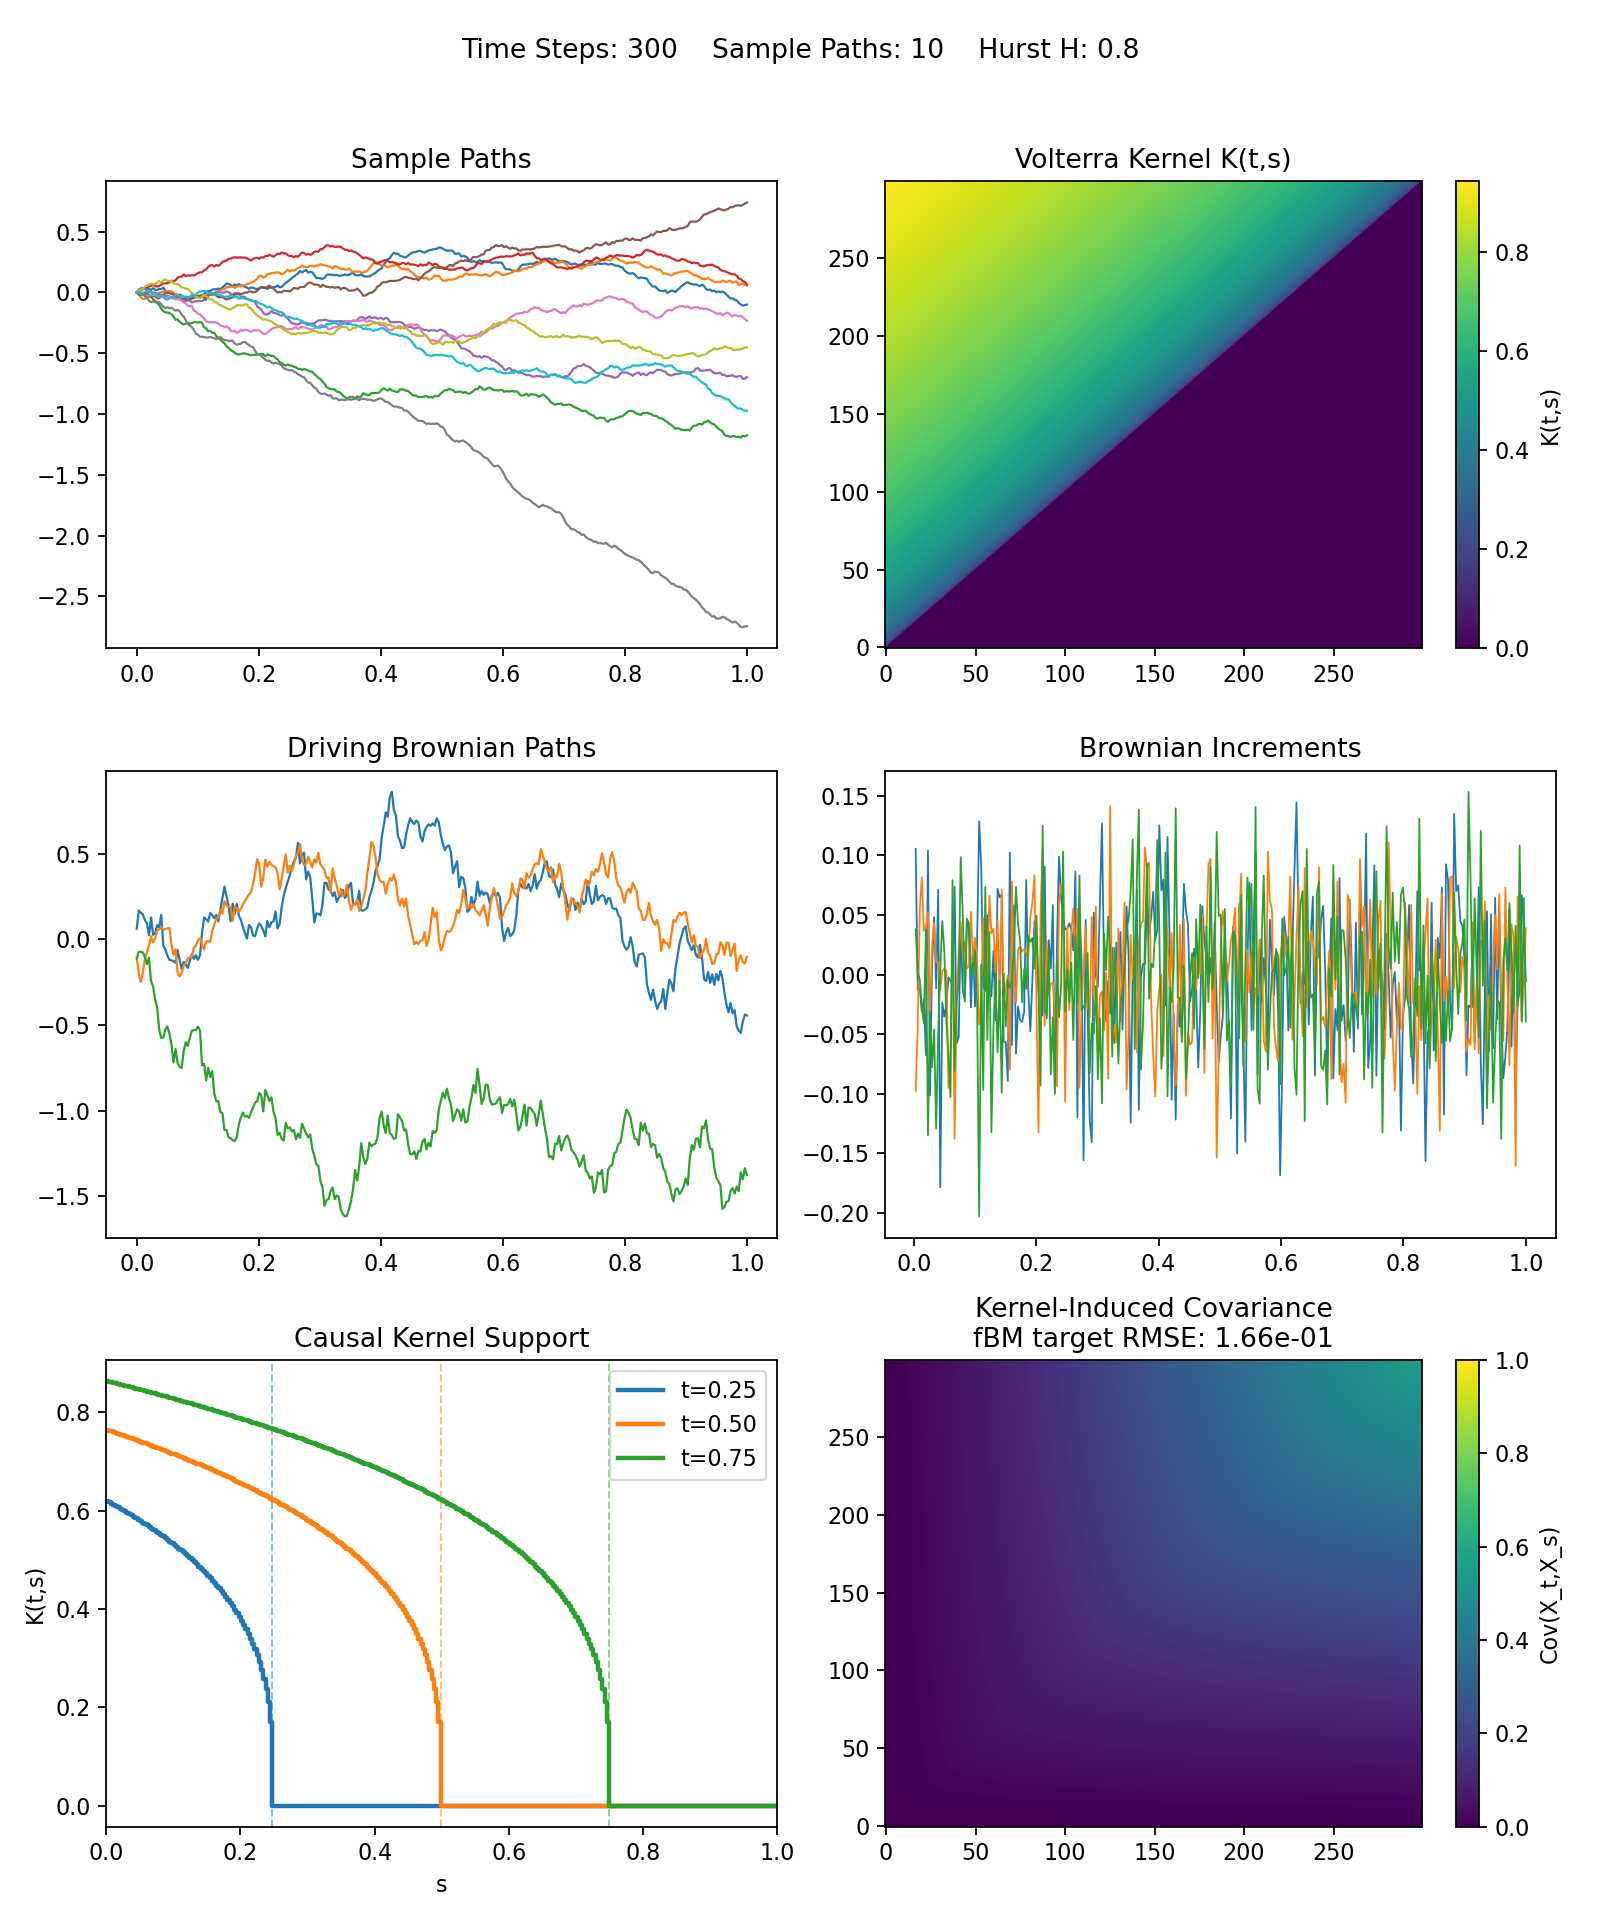
\includegraphics[width=\linewidth]{img/hft2-volterra0_8.png}
\end{minipage}
\hfill
\begin{minipage}[t]{0.42\textwidth}
\vspace{0pt}
\normalsize


\textbf{Persistent regime: \(H=0.8\).}

When \(H>\tfrac12\), the kernel becomes smoother and the relative importance of more distant history increases. The process still has a causal representation, since only past noise is used, but the accumulated effect of history now produces much smoother and more persistent trajectories. This is visible both in the iterative construction and in the full Volterra diagnostics: the paths display stronger directional continuity, and the covariance pattern becomes more persistent across time indices.

\vspace{0.5cm}
\centering
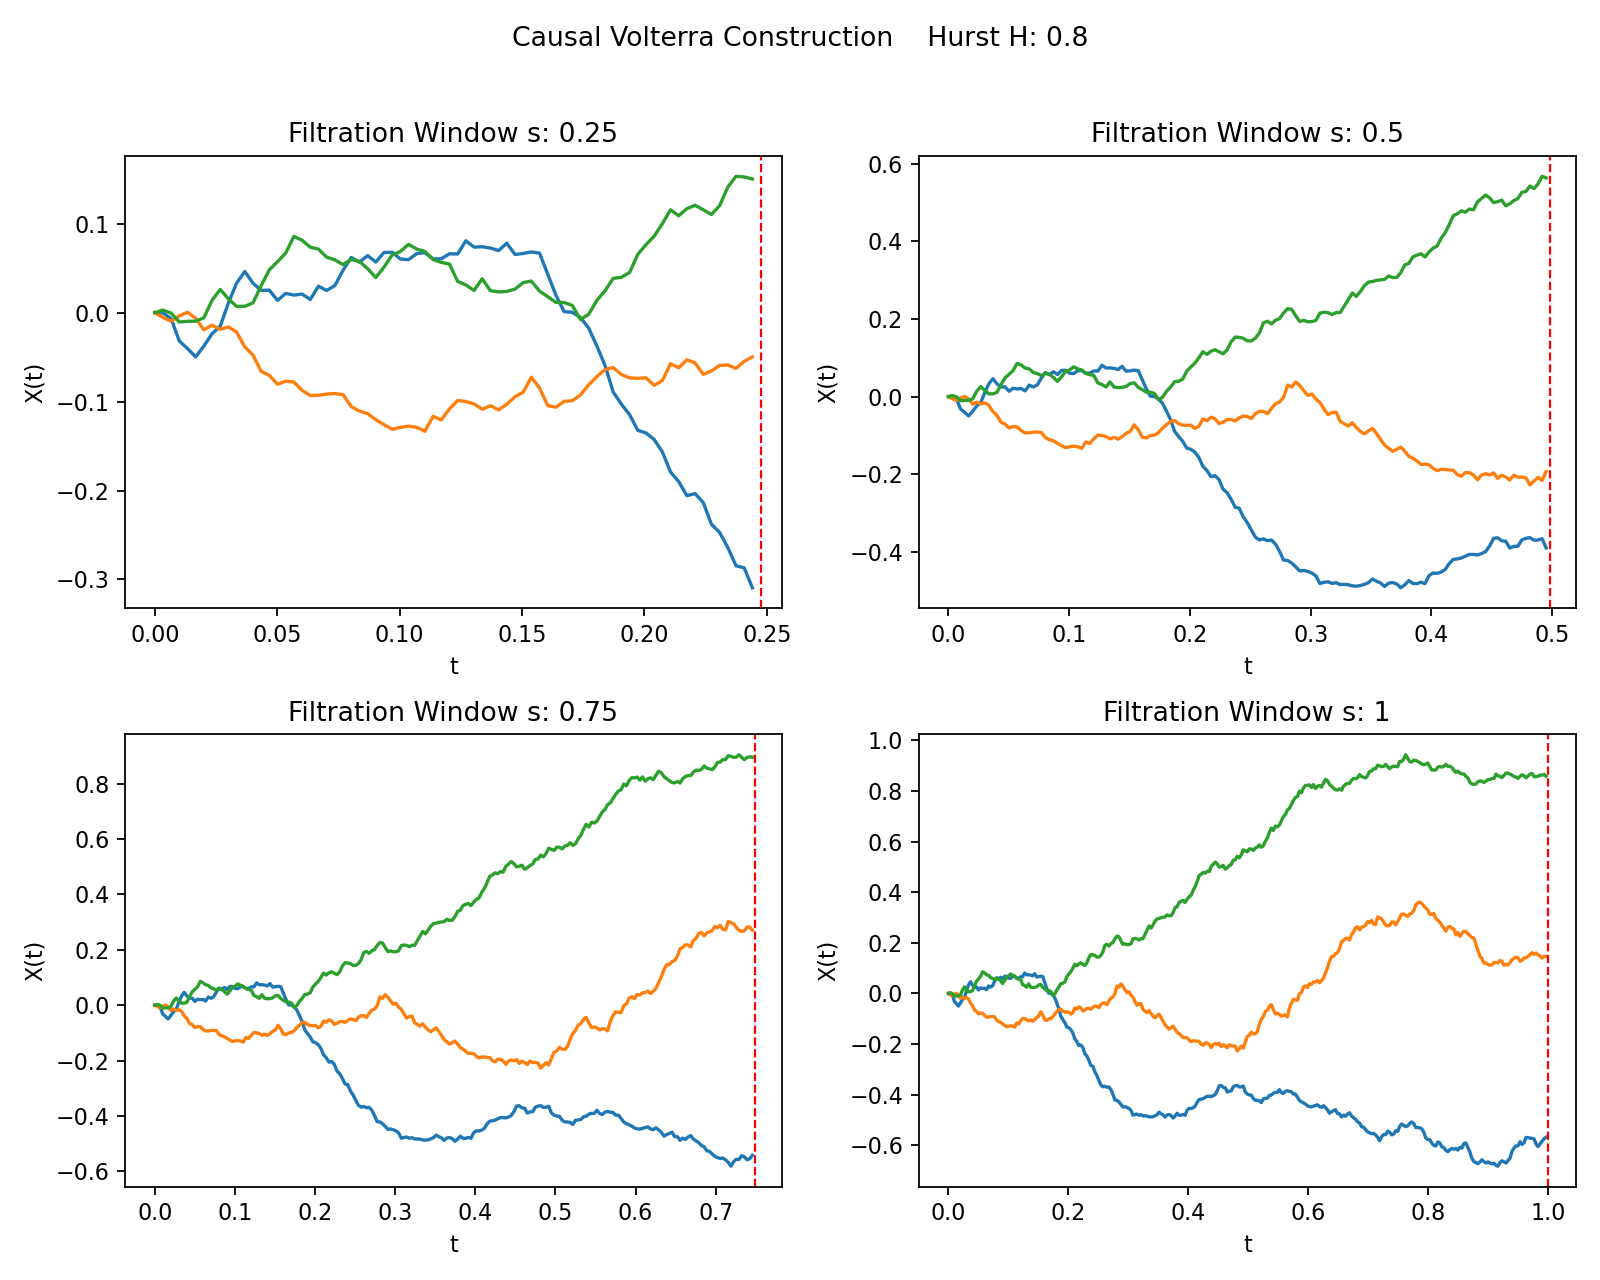
\includegraphics[width=\linewidth]{img/hft2-iterative0_8.png}
\end{minipage}
\end{figure}
\clearpage
\paragraph{Implementation.}

A convenient way to simulate a Volterra process numerically is to implement a generic routine that accepts a kernel as an argument. This makes it possible to recover Brownian motion, Ornstein--Uhlenbeck dynamics, or fractional-type processes simply by changing the kernel.

This implementation is intentionally generic. If one calls the simulator with \texttt{brownian\_kernel}, the output is a Brownian path written in Volterra form. If one uses \texttt{ou\_kernel(theta)}, the output becomes an Ornstein--Uhlenbeck process. If one uses \texttt{fractional\_kernel(H)}, the output is a causal fractional-type Volterra process whose roughness and persistence are controlled by \(H\).

\paragraph{Computational cost and transition to lifting.}

The Volterra representation solves the causality problem, but it does not eliminate the memory problem. To compute \(X_{t_i}\), one still has to survey the entire history of shocks \(\Delta W_0,\dots,\Delta W_{i-1}\). As a consequence, the cost per path grows roughly quadratically in the number of time steps:
\[
\text{cost per path} \sim O(n^2).
\]
This is acceptable for a theoretical laboratory and for moderate Monte Carlo experiments, but it becomes expensive once the process is embedded inside calibration loops, filtering procedures, or control problems.

The important gain is therefore structural rather than asymptotic: Volterra processes are causal, interpretable, and directly suited to sequential simulation. Their remaining computational bottleneck is exactly what motivates the next step of the paper. If the kernel can be approximated by a finite mixture of exponentials, the process can be rewritten in an enlarged but finite-dimensional Markovian state space. This is the idea behind Markovian lifting, which preserves the rough-memory intuition while recovering a tractable recursive structure for simulation and control.

%%%%%%%%%%%%%%%%%%%%%%%%%%%%%%%%%%%%%%%%%%%%%%%%
%%%%%%%%%%%%%%%%%%%%%%%%%%%%%%%%%%%%%%%%%%%%%%%%
%%%%%%%%%%%%%%%%%%%%%%%%%%%%%%%%%%%%%%%%%%%%%%%%

The singular-memory kernel is not solved by relabeling its scalar output as a Markov state. The next chapter replaces it by a finite sum of exponentials and retains all factor coordinates. This recovers recursion for the approximating model, while leaving the kernel approximation and any subsequent state compression visible.

\chapter{Finite Markovian Lifts and Scalar Compression}\label{ch:lift}
A non-Markovian memory model and its finite Markovian approximation must be distinguished. A sum of exponential kernels introduces recursive OU factors. The full factor vector is Markovian; its weighted aggregate generally is not a closed scalar Markov process when decay rates differ. This chapter connects the kernel construction to the information discarded by a small control grid.
\section{Markovian Lifting}


\paragraph{Why lifting is needed.}

A Markov process has the property that the future depends on the present state alone. This is precisely what makes Brownian-motion-based models so efficient computationally: when one wants to generate the next step of the path, the whole history is not needed. By contrast, rough and fractional models are designed to preserve memory. In a Volterra representation,
\[
X_t=\int_0^t K(t,s)\,dW_s,
\]
the kernel \(K\) makes the current state depend on the entire past trajectory of the driving noise. This is mathematically attractive, but it destroys the simple recursive structure that is available in a Markov model.

One could always make the path itself part of the state, but that would not really solve anything. Expanding the state space to include the entire history is exact, yet it is not a simplification. The idea of Markovian lifting is more selective: instead of keeping the full path, one approximates the effect of the path by a finite collection of auxiliary state variables that are themselves Markovian. In this way, one retains the main covariance features of the rough dynamics without carrying the full historical trajectory at every step.

\subsection{Why exponentials are special}

The key mathematical reason lifting works is that exponentials satisfy a semigroup property. For any \(x>0\),
\[
e^{-x(t+\Delta t-s)} = e^{-x\Delta t}e^{-x(t-s)}.
\]
This simple identity is enough to recover a Markov recursion. To see it, define for a fixed rate \(x>0\) the auxiliary process
\[
U_t(x)=\int_0^t e^{-x(t-s)}\,dW_s.
\]
Then
\[
U_{t+\Delta t}(x)
=
\int_0^{t+\Delta t} e^{-x(t+\Delta t-s)}\,dW_s.
\]
Splitting the integral at time \(t\) and applying the semigroup property gives
\[
U_{t+\Delta t}(x)
=
e^{-x\Delta t}\int_0^t e^{-x(t-s)}\,dW_s
+
\int_t^{t+\Delta t} e^{-x(t+\Delta t-s)}\,dW_s,
\]
hence
\[
U_{t+\Delta t}(x)
=
e^{-x\Delta t}U_t(x)
+
\int_t^{t+\Delta t} e^{-x(t+\Delta t-s)}\,dW_s.
\]
The first term depends only on the current state \(U_t(x)\), while the second term depends only on the new Brownian increment over \([t,t+\Delta t]\). This is exactly the structure of a Markov update.

This mechanism fails for a pure power law. If one considers a rough kernel of the form
\[
(t-s)^{\alpha-1},
\]
then in general
\[
(t+\Delta t-s)^{\alpha-1}
\neq
(\Delta t)^{\alpha-1}(t-s)^{\alpha-1}.
\]
The semigroup property is absent, and this is the algebraic reason why pure rough kernels remain non-Markovian.

\subsection{Laplace representation of the rough kernel}

The rough-volatility kernel is typically written in the power-law form
\[
K_\alpha(\tau)=\frac{\tau^{\alpha-1}}{\Gamma(\alpha)},
\qquad
\alpha\in\left(\frac12,1\right),
\qquad
\tau>0.
\]
If one writes \(\alpha=H+\tfrac12\), then the rough regime corresponds to \(H\in(0,\tfrac12)\). The key observation behind lifting is that this kernel can be represented as a Laplace transform of exponential functions.

\begin{proposition}[Laplace representation of the power-law kernel]
For \(\alpha\in(0,1)\) and \(\tau>0\),
\[
\frac{\tau^{\alpha-1}}{\Gamma(\alpha)}
=
\frac{1}{\Gamma(\alpha)\Gamma(1-\alpha)}
\int_0^\infty e^{-\lambda \tau}\lambda^{-\alpha}\,d\lambda.
\]
Using Euler's reflection formula,
\[
\frac{1}{\Gamma(\alpha)\Gamma(1-\alpha)}
=
\frac{\sin(\pi\alpha)}{\pi},
\]
so equivalently
\[
\frac{\tau^{\alpha-1}}{\Gamma(\alpha)}
=
\frac{\sin(\pi\alpha)}{\pi}
\int_0^\infty e^{-\lambda \tau}\lambda^{-\alpha}\,d\lambda.
\]
\end{proposition}

\begin{proof}
By definition of the Gamma function,
\[
\Gamma(1-\alpha)=\int_0^\infty u^{-\alpha}e^{-u}\,du.
\]
Now make the substitution \(u=\lambda \tau\), so that \(du=\tau\,d\lambda\). Then
\[
\Gamma(1-\alpha)
=
\int_0^\infty (\lambda\tau)^{-\alpha}e^{-\lambda\tau}\tau\,d\lambda
=
\tau^{1-\alpha}\int_0^\infty \lambda^{-\alpha}e^{-\lambda\tau}\,d\lambda.
\]
Dividing both sides by \(\tau^{1-\alpha}\Gamma(\alpha)\Gamma(1-\alpha)\) gives
\[
\frac{\tau^{\alpha-1}}{\Gamma(\alpha)}
=
\frac{1}{\Gamma(\alpha)\Gamma(1-\alpha)}
\int_0^\infty e^{-\lambda\tau}\lambda^{-\alpha}\,d\lambda.
\qedhere
\]
\end{proof}

This identity is the analytical foundation of Markovian lifting. A singular power-law kernel can be interpreted as a continuous mixture of exponential kernels, and each exponential kernel corresponds to one mean-reverting Markov factor.

\subsection{From a continuous mixture to a finite lifted state}

The continuous Laplace representation is still infinite-dimensional. To obtain a practical model, one replaces the integral over \(\lambda\) by a finite quadrature rule. Choose rates
\[
\lambda_1,\dots,\lambda_M>0
\]
and positive weights
\[
w_1,\dots,w_M>0.
\]
Then approximate the rough kernel by
\[
K_\alpha(\tau)\approx K_\alpha^{(M)}(\tau)
=
\sum_{k=1}^M w_k e^{-\lambda_k \tau}.
\]
The corresponding lifted process becomes
\[
Y_t^{(M)}
=
\int_0^t K_\alpha^{(M)}(t-s)\,dW_s
=
\sum_{k=1}^M w_k U_t^{(k)},
\]
where
\[
U_t^{(k)}
=
\int_0^t e^{-\lambda_k(t-s)}\,dW_s.
\]
Each factor \(U^{(k)}\) is an Ornstein--Uhlenbeck-type Gaussian state satisfying
\[
dU_t^{(k)}=-\lambda_k U_t^{(k)}\,dt + dW_t,
\qquad
U_0^{(k)}=0.
\]
The entire lifted state is therefore
\[
Z_t=\bigl(U_t^{(1)},\dots,U_t^{(M)}\bigr)^\top,
\]
which is finite-dimensional and Markovian.

This is the core idea of lifting: instead of carrying an infinite-dimensional Volterra memory, one works with a stack of \(M\) mean-reverting factors. The model is no longer exact at finite \(M\), but it regains the recursive structure that is lost in the rough Volterra formulation.

\paragraph{Why this matters for rough volatility.}

The relevance of lifting is especially clear in rough-volatility models. A prototypical rough variance process may be written schematically as
\[
V_t
=
V_0
+
\int_0^t K_\alpha(t-s)\,dZ_s,
\]
where \(Z\) collects the drift and volatility-of-volatility terms. The non-Markovian difficulty comes entirely from the kernel \(K_\alpha\). Once \(K_\alpha\) is replaced by its finite exponential approximation \(K_\alpha^{(M)}\), the same variance process can be written as a linear combination of \(M\) Markovian factors:
\[
V_t
\approx
V_0+\sum_{k=1}^M w_k U_t^{(k)}.
\]
This is the step that restores the affine-type structure and makes fast simulation feasible again. In other words, lifting does not eliminate roughness by ignoring it; it replaces roughness by a structured finite-dimensional approximation that can still be handled recursively.

\subsection{Discrete-time recursion}

Fix a uniform grid
\[
t_i=i\Delta t,
\qquad i=0,\dots,n,
\qquad \Delta t=\frac{T}{n}.
\]
For each OU factor, the exact one-step transition is
\[
U_{i+1}^{(k)}=e^{-\lambda_k\Delta t}U_i^{(k)}+\eta_{i+1}^{(k)},
\]
where the innovation vector
\[
\eta_{i+1}=
\bigl(\eta_{i+1}^{(1)},\dots,\eta_{i+1}^{(M)}\bigr)^\top
\]
is centered Gaussian. Because all factors are driven by the same Brownian motion, these innovations are correlated, with covariance
\[
\Cov\!\bigl(\eta^{(j)},\eta^{(k)}\bigr)
=
\frac{1-e^{-(\lambda_j+\lambda_k)\Delta t}}{\lambda_j+\lambda_k}.
\]
After updating the factors, the lifted process is reconstructed by
\[
Y_i^{(M)}=\sum_{k=1}^M w_k U_i^{(k)}.
\]

An equivalent weighted-state representation is also possible. One may define
\[
X_t^{(k)}:=w_k U_t^{(k)},
\]
so that
\[
dX_t^{(k)}=-\lambda_k X_t^{(k)}\,dt+w_k\,dW_t,
\qquad
Y_t^{(M)}=\sum_{k=1}^M X_t^{(k)}.
\]
In that convention, the innovation covariance becomes
\[
\Cov\!\bigl(\eta^{(j)},\eta^{(k)}\bigr)
=
w_jw_k\,
\frac{1-e^{-(\lambda_j+\lambda_k)\Delta t}}{\lambda_j+\lambda_k}.
\]
Both formulations are equivalent as long as the weights are used consistently.

\subsection{Practical construction of the lift}

\paragraph{Rates and weights.}

The finite approximation depends on the choice of quadrature nodes \(\lambda_k\) and weights \(w_k\). A common practical heuristic is to use log-spaced rates,
\[
\lambda_k \in \left[\frac{2}{T},\frac{400}{T}\right],
\]
and weights proportional to
\[
w_k \propto \lambda_k^{-(H+\frac12)}.
\]
This mirrors the Laplace-domain mass of the rough kernel and usually provides a reasonable first approximation. However, this choice is heuristic rather than optimal. In particular, the approximation error is not guaranteed to decrease monotonically with \(M\), and in finite samples the empirical covariance RMSE may oscillate because of three interacting effects:
\begin{itemize}
    \item approximation error from the finite exponential mixture,
    \item Monte Carlo noise from the simulated covariance matrix,
    \item numerical conditioning effects when the factor system becomes larger.
\end{itemize}

For this reason, one should interpret the lifting dimension \(M\) as a bias--variance trade-off rather than as a parameter for which ``larger is always better''. In practice, a moderate value often gives the most stable overall result.

\paragraph{Discrete-time recipe.}

A convenient summary of the lifting procedure is the following:

\begin{enumerate}[label=\arabic*.]
    \item Choose a Hurst parameter \(H\in(0,1)\) and a lifting dimension \(M\).
    \item Define a time grid \(t_i=i\Delta t\) on \([0,T]\).
    \item Select mean-reversion rates \(\lambda_1,\dots,\lambda_M\), typically on a log scale.
    \item Choose weights \(w_1,\dots,w_M\) from a Laplace-domain quadrature heuristic.
    \item Build the Gaussian innovation covariance matrix of the OU factors.
    \item Simulate the factor recursion
    \[
    U_{i+1}^{(k)}=e^{-\lambda_k\Delta t}U_i^{(k)}+\eta_{i+1}^{(k)}.
    \]
    \item Aggregate the factors through
    \[
    Y_i^{(M)}=\sum_{k=1}^M w_k U_i^{(k)}.
    \]
\end{enumerate}

When the objective is to compare the lifted process directly with fractional Brownian motion on a fixed grid, it is often useful to rescale each time column so that the marginal variance matches
\[
\Var(B_t^H)=t^{2H}.
\]
This does not turn the lift into exact fractional Brownian motion. It simply isolates the covariance-shape approximation from a mismatch in marginal scale.

\paragraph{Implementation.}

This implementation keeps the OU factors unweighted internally and applies the weights only at aggregation. The function \texttt{match\_fbm\_marginals} can then be used when the goal is a direct visual or covariance comparison with fractional Brownian motion on a fixed discrete grid.

\subsection{Visual comparison across Hurst parameters}

The panels below illustrate the lifted approximation for three representative values of the Hurst parameter. In each composite image, the main lifted covariance is shown together with the target fractional covariance and a lag-wise covariance-error profile. The smaller diagnostic panels also compare nearby lifting dimensions, which makes it possible to see that the empirical error does not necessarily decrease monotonically as the number of OU factors changes.

The important point is therefore not a perfectly monotone RMSE sequence, but rather the overall stability of the approximation. Across repeated simulations, the empirical covariance error oscillates because it is itself a Monte Carlo object. 

The case $H=0.8$ is included as a persistent stress regime for the numerical comparison. It lies outside the standard empirically rough range $H<\tfrac12$ covered by the singular-kernel argument above, so it should not be read as a claim that persistent volatility is rough in the usual sense.

\begin{algorithm}[H]
\caption{Reading the Markovian-lifting diagnostic panels}
\DontPrintSemicolon
choose \(H\), a factor count \(M\), rates \(\lambda_k\), and weights \(w_k\)\;
simulate the correlated OU-factor recursion for the lifted state\;
aggregate \(Y^{(M)}=\sum_k w_k U^{(k)}\) and match the marginal scale when comparing with \(B^H\)\;
estimate the lifted covariance, compare it with the fractional target, and plot the lag-wise error\;
\end{algorithm}

Nevertheless, the error remains controlled, the qualitative geometry of the covariance surface is preserved, and the lift continues to reproduce the broad persistence pattern of the target process. In particular, the roughest regime is the hardest one to approximate, while smoother regimes are matched more easily.

\begin{figure}[H]
\centering
\begin{minipage}[t]{0.47\textwidth}
\vspace{0pt}
\normalsize

\vspace{0.25cm}

\textbf{Benchmark regime: \(H=0.5\).}

This is the intermediate benchmark case. The lifted covariance already captures the broad triangular structure of the target fractional covariance, but the lag-wise error profile shows that the approximation is still imperfect. The nearby factor-count diagnostics included in the panel also illustrate a practical point: changing the number of OU factors does not produce a strictly monotone reduction of the empirical RMSE. In repeated runs, the error oscillates because approximation error and Monte Carlo noise interact, but it remains controlled and the overall covariance geometry is preserved.

\end{minipage}
\hfill
\begin{minipage}[t]{0.47\textwidth}
\vspace{0pt}
\centering
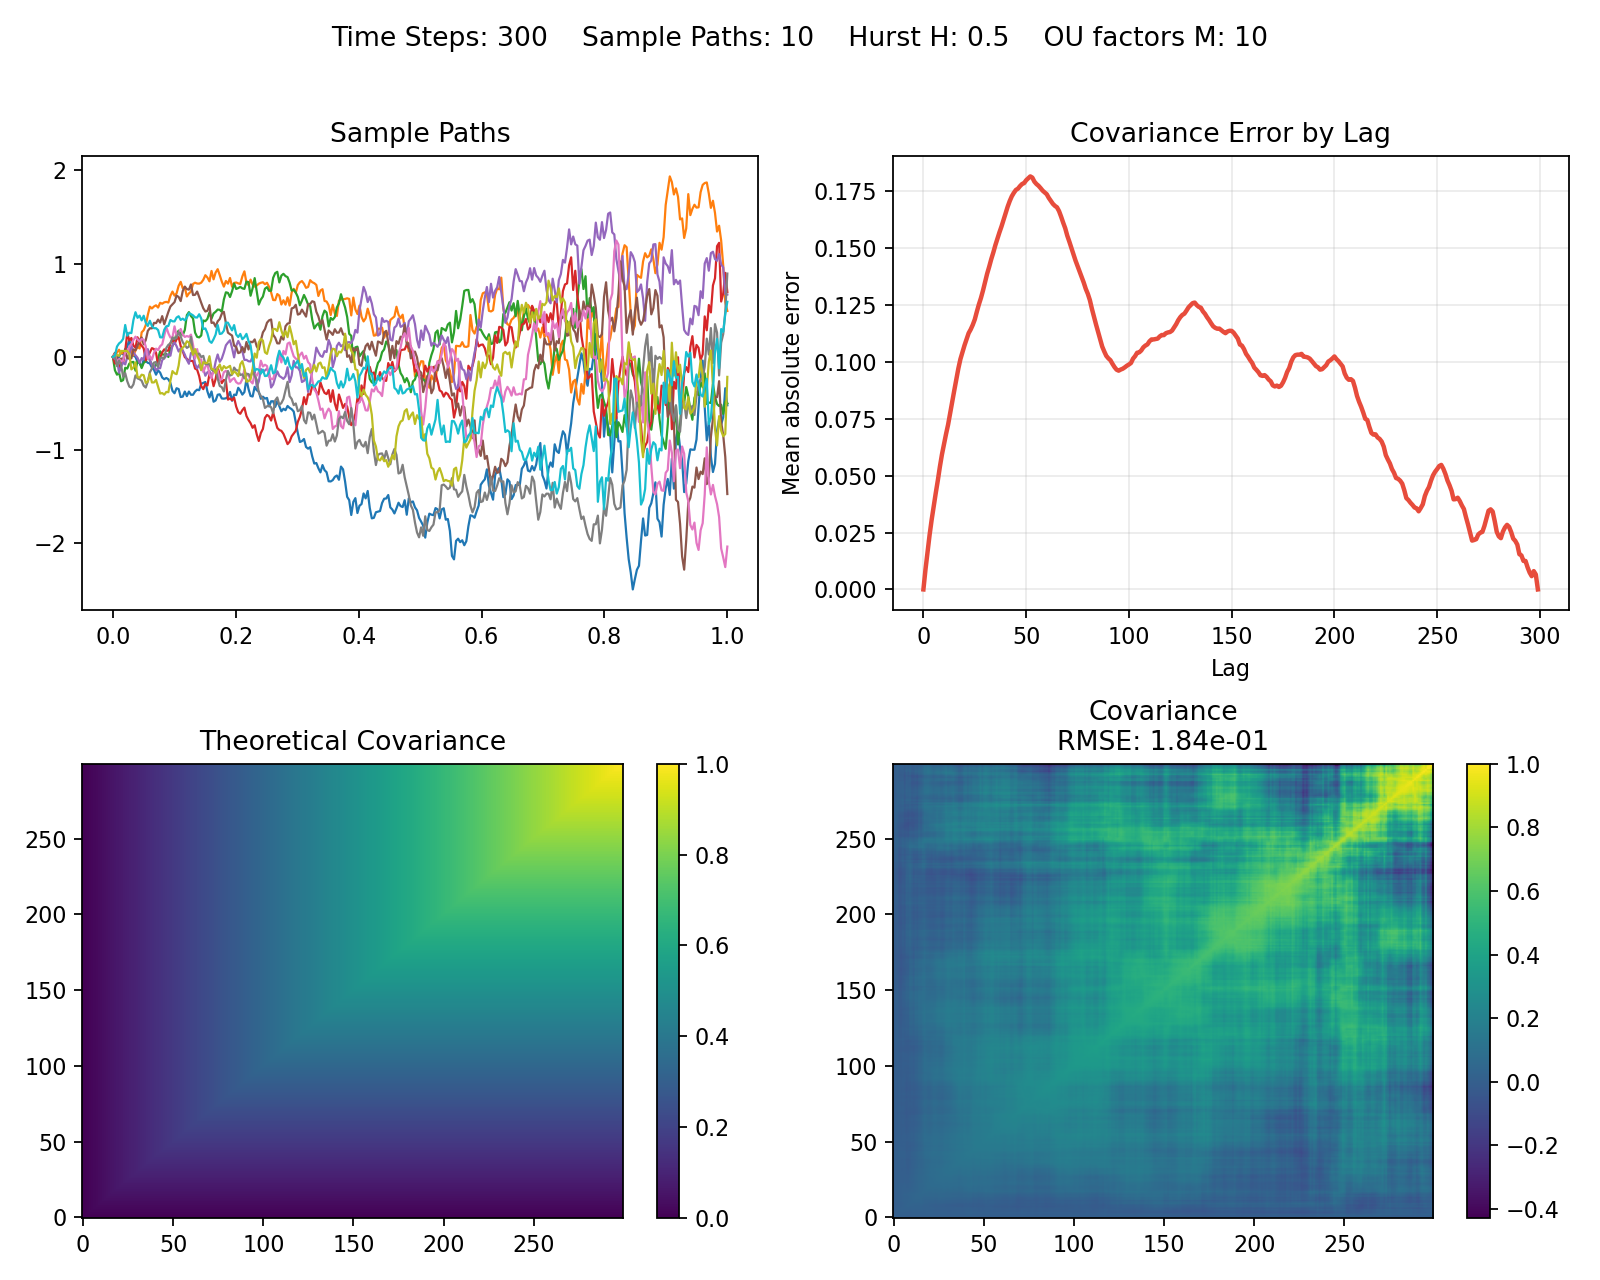
\includegraphics[width=6.5cm]{img/hft2-ML0_5.png}
\end{minipage}
\end{figure}

\begin{figure}[H]
\centering
\begin{minipage}[t]{0.47\textwidth}
\vspace{0pt}
\centering
%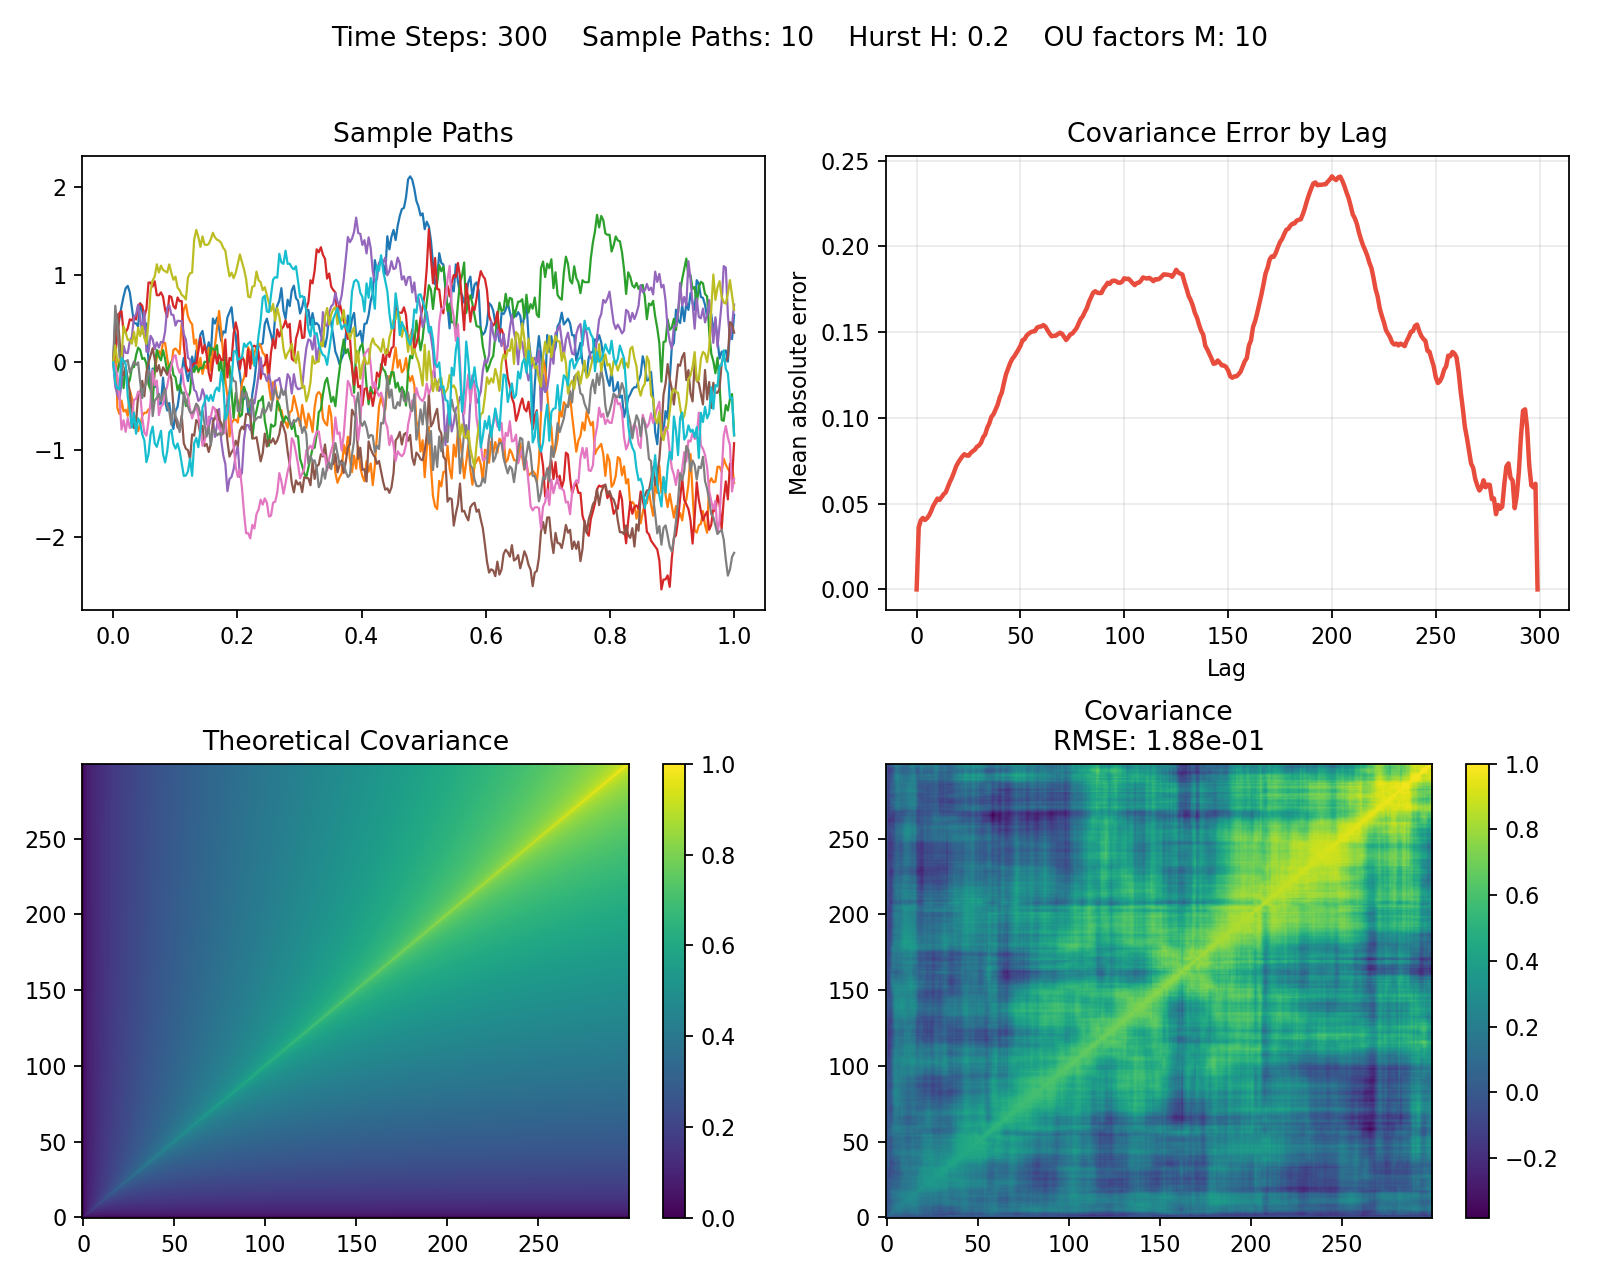
\includegraphics[width=\linewidth]{img/hft2-ML0_2.png}
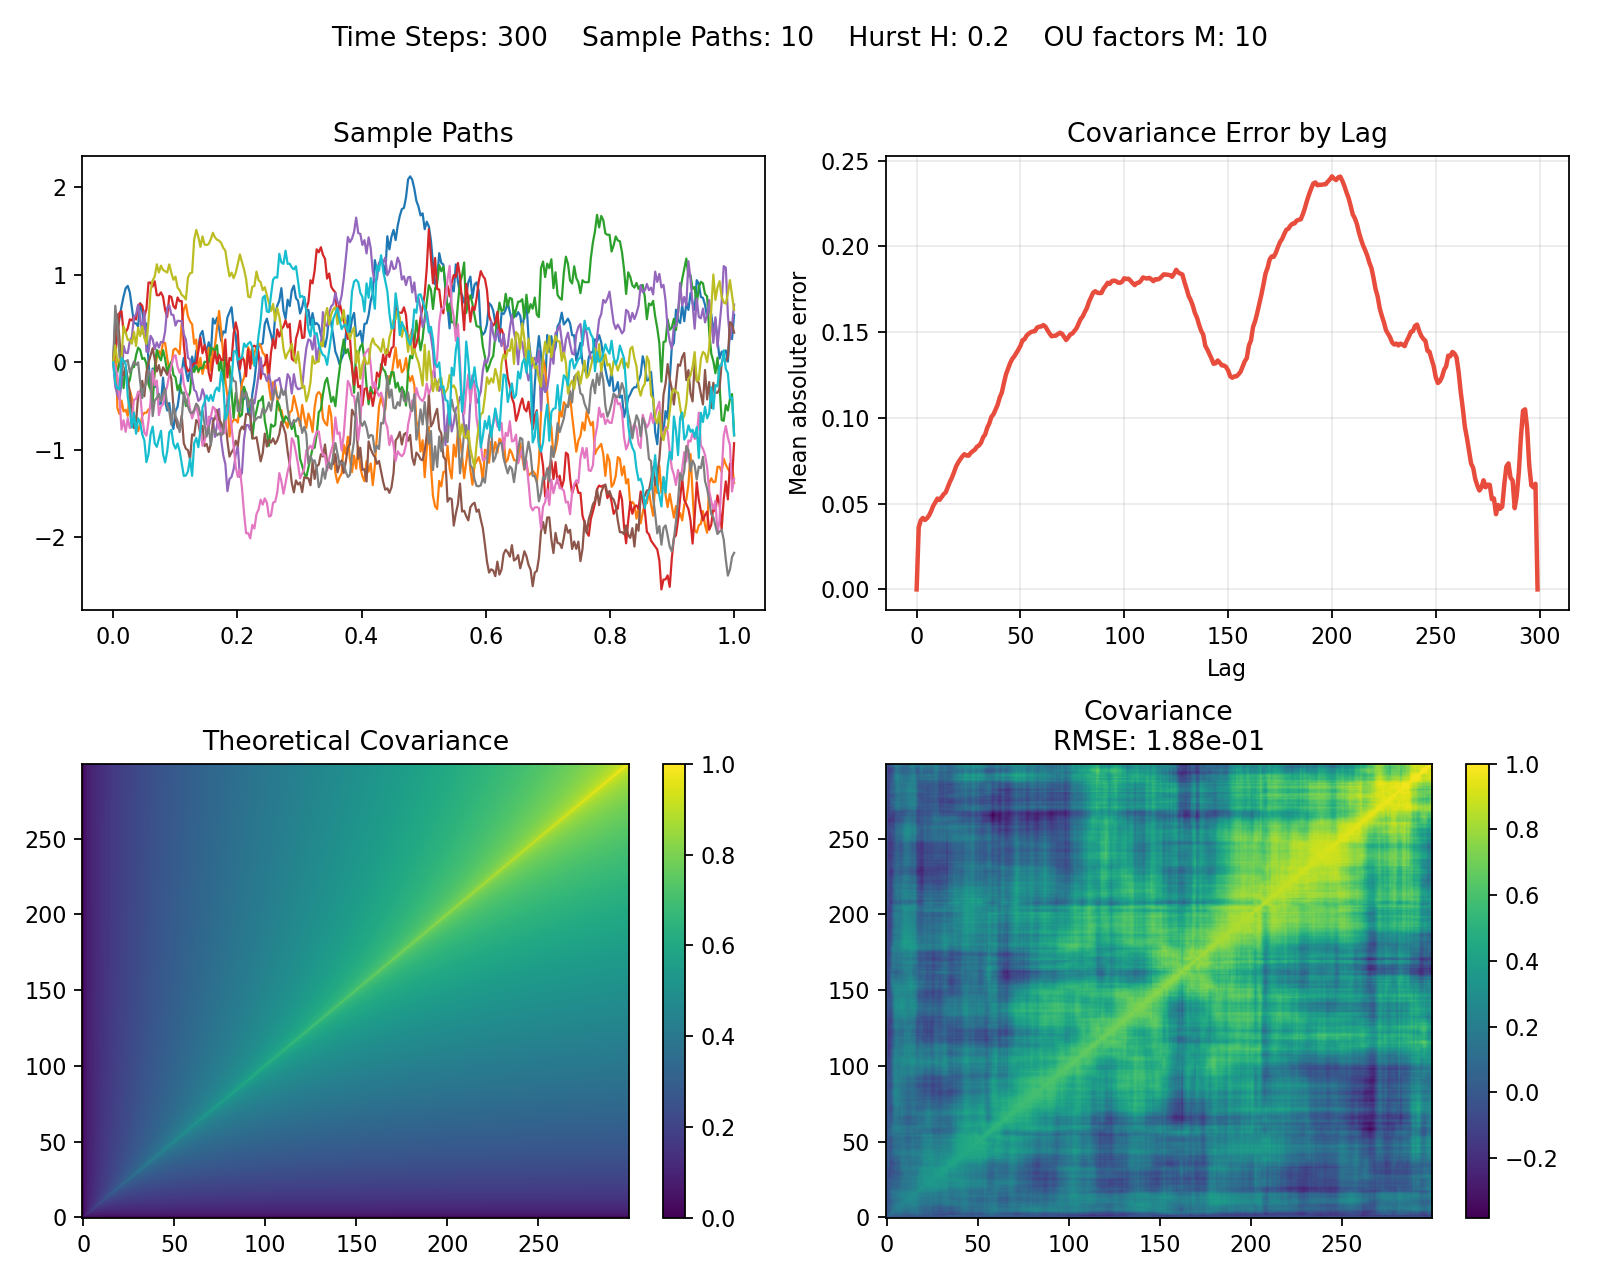
\includegraphics[width=6.5cm]{img/hft2-ML0_2.png}
\end{minipage}
\hfill
\begin{minipage}[t]{0.47\textwidth}
\vspace{0pt}
\normalsize
\textbf{Rough regime: \(H=0.2\).}

This is the most challenging case. Because the target covariance is generated by a much rougher kernel, a finite exponential mixture has a harder task: the lifted approximation still reproduces the global covariance pattern, but the empirical RMSE is larger and the lag-wise error is more pronounced. This should not be interpreted as a failure of the method. Rather, it shows that the roughest regime is the one in which the finite-dimensional approximation is under the greatest pressure. Even here, however, repeated simulation does not produce unstable behavior: %the error fluctuates from run to run, but remains bounded and the target covariance shape is still clearly recognizable.
\end{minipage}
\end{figure}

the error fluctuates from run to run, but remains bounded and the target covariance shape is still clearly recognizable.

\begin{figure}[H]
\centering
\begin{minipage}[t]{0.47\textwidth}
\vspace{0.25cm}
\normalsize
\textbf{Persistent regime: \(H=0.8\).}

When \(H>\tfrac12\), the target covariance is smoother and the lifted approximation becomes noticeably easier. This is reflected both in the heat maps and in the much smaller lag-wise covariance error. In this regime the exponential mixture is already rich enough to track the target geometry rather closely. As before, the RMSE observed in simulation is not perfectly deterministic across runs, but its oscillations remain small and the approximation is visibly more accurate than in the rough case.


\end{minipage}
\hfill
\begin{minipage}[t]{0.47\textwidth}
\vspace{0pt}
\centering
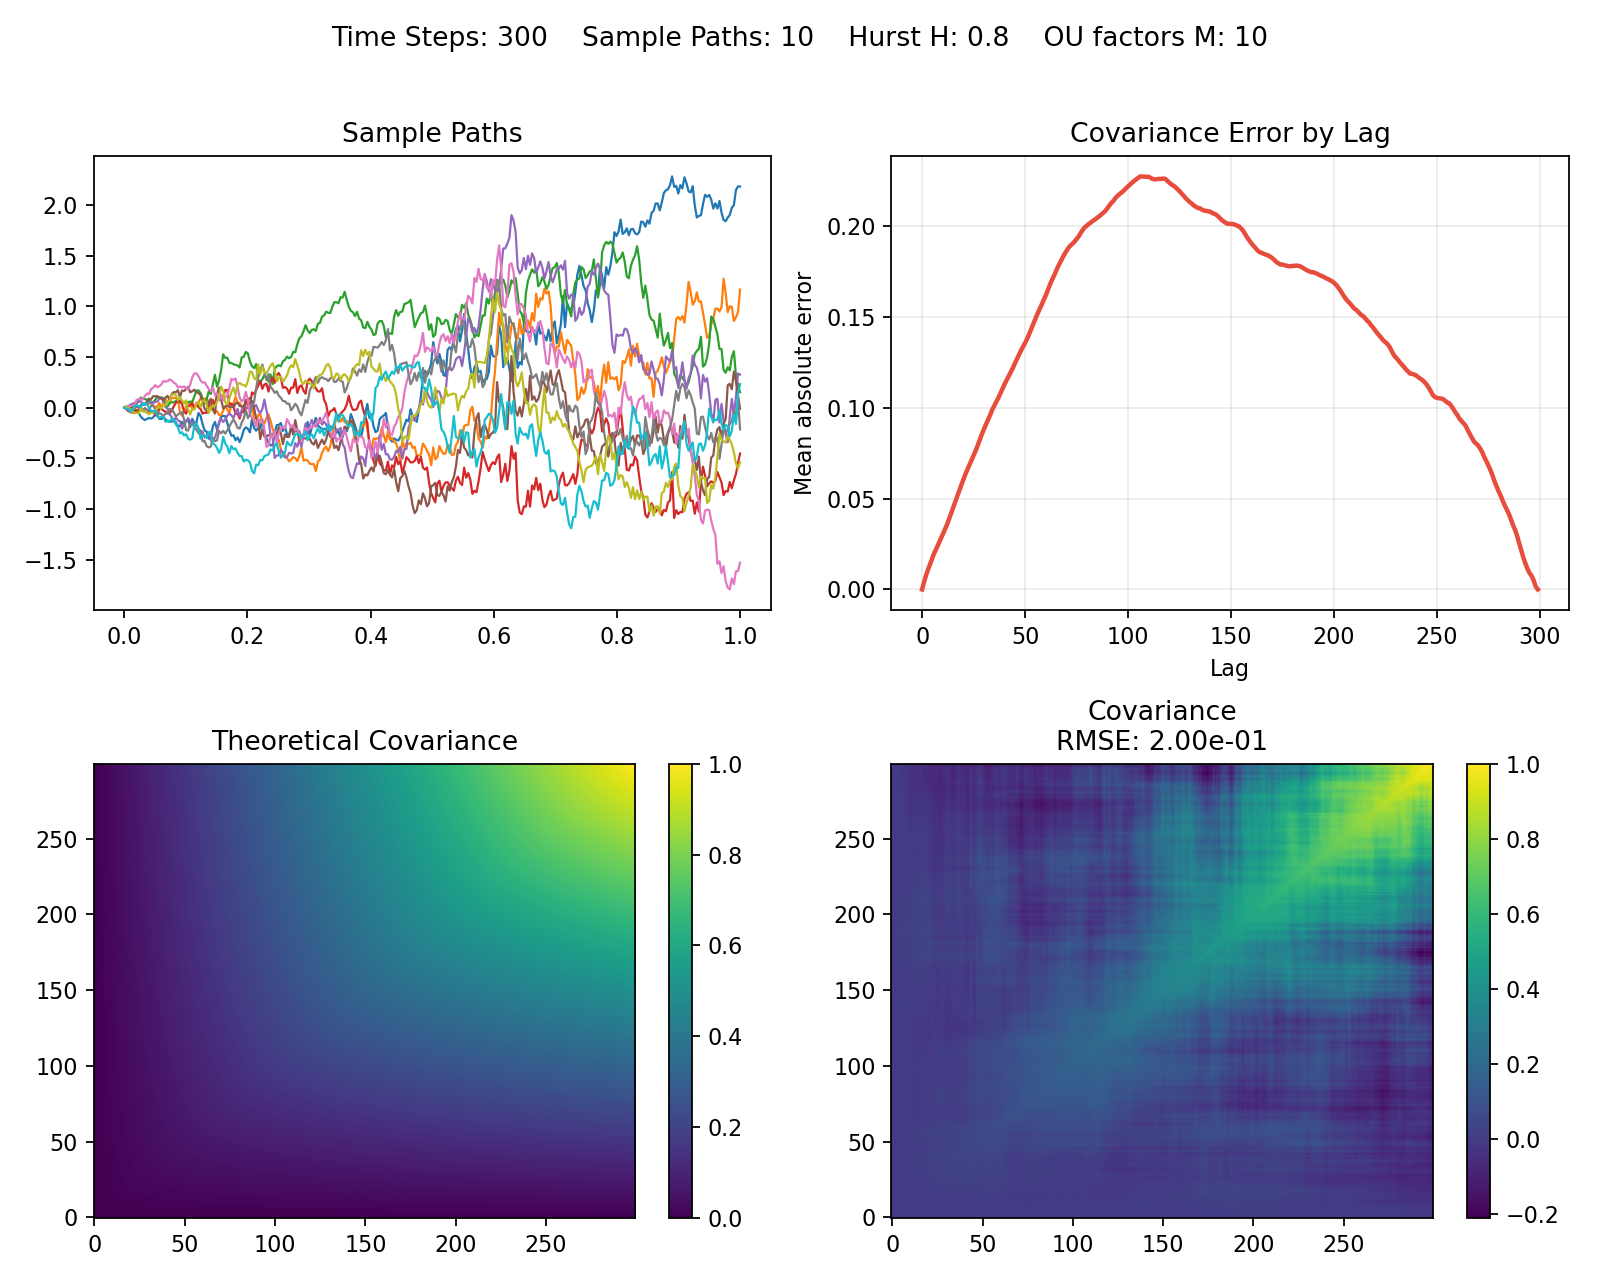
\includegraphics[width=6.5cm]{img/hft2-ML0_8.png}
\end{minipage}
\end{figure}

\subsection{What lifting solves, and what it does not solve}

Markovian lifting does not make the process exactly equal to fractional Brownian motion at finite \(M\). That would be too strong a claim. What it does is much more practical: it replaces a non-Markovian singular-memory dynamics by a finite-dimensional Markov approximation that preserves the main covariance features sufficiently well for simulation and control.

This distinction matters. The purpose of lifting is not exact identity at fixed factor dimension, but tractability. The rough memory is compressed into a finite state vector,
\[
Z_t=\bigl(U_t^{(1)},\dots,U_t^{(M)}\bigr)^\top,
\]
and this state can be updated recursively. That is precisely what makes the method attractive for repeated Monte Carlo simulation, calibration to liquid instruments, and eventually inventory control inside a market-making engine.

From the perspective of this study, Markovian lifting is therefore the final step in the mathematical transition
\[
\text{fractional covariance}
\quad\longrightarrow\quad
\text{causal Volterra representation}
\quad\longrightarrow\quad
\text{finite-dimensional Markov state}.
\]
The following volatility mapping uses this state-space perspective to reconnect the rough driver with a volatility process and, ultimately, with the reservation-price logic of a rough-volatility Avellaneda--Stoikov model.

\section{From Rough Paths to Rough Volatility}


The modeling task is now operational. A lifted rough state must be embedded inside a positive volatility process without breaking the recursive simulation architecture, and the resulting variance forecast must be translated into an inventory-aware quoting rule.

\subsection{From a lifted rough state to a volatility factor}

Let
\[
Y_t^{(M)}=\sum_{k=1}^M w_k U_t^{(k)}
\]
denote the lifted Gaussian rough state obtained in the previous chapter, where the factors \(U^{(k)}\) satisfy OU-type dynamics. By construction, \(Y_t^{(M)}\) is Gaussian and can take both positive and negative values. For that reason, it should not be interpreted directly as a variance process. A separate link function is needed to map the rough state into a positive volatility or variance input.

There are two natural modeling routes.

The first is structural and closer to the rough-Heston literature. In that case one thinks of volatility as a Volterra-type process driven by a rough kernel, for example
\[
V_t
=
V_0
+
\int_0^t
K_\alpha(t-s)
\Bigl(
\kappa(\theta-V_s)\,ds
+
\xi\sqrt{V_s}\,dW_s^v
\Bigr),
\qquad
K_\alpha(\tau)=\frac{\tau^{\alpha-1}}{\Gamma(\alpha)},
\]
with \(\alpha=H+\tfrac12\in(\tfrac12,1)\). This specification is conceptually important because it shows how rough memory enters variance directly. However, for the control problem it is not necessary to solve the full rough-Heston calibration problem in order to study market-making control.

The second route is more practical and better aligned with a simulation-first HFT study. One treats the lifted rough state as a latent Gaussian driver for log-volatility and defines, for example,
\[
\log v_t = m_t + \beta Y_t^{(M)},
\]
or equivalently
\[
v_t = \exp\!\bigl(m_t+\beta Y_t^{(M)}\bigr),
\]
where \(m_t\) is a deterministic baseline level and \(\beta>0\) controls the sensitivity of volatility to the rough factor. This choice guarantees positivity and preserves the intuition that large positive realizations of the rough state generate volatility clusters. It is also numerically convenient, because once the lifted factor has been simulated, the volatility process is obtained pointwise with no additional memory burden.

A slightly more stable centered version is
\[
v_t
=
\bar v\,
\exp\!\left(
\beta Y_t^{(M)}
-\frac12\beta^2\Var(Y_t^{(M)})
\right),
\]
which normalizes the unconditional level around \(\bar v\). The point is not that this is the only admissible specification, but that it turns the lifted state into a positive and simulation-ready volatility input.

\paragraph{Rough-volatility mid-price dynamics.}

Once a positive volatility process \(v_t\) has been constructed, the mid-price can be modeled by
\[
dS_t = \mu_t\,dt + \sqrt{v_t}\,dW_t^S,
\]
possibly with correlation between the price noise \(W^S\) and the volatility noise \(W^v\) or, in the lifted setting, between \(W^S\) and the Brownian driver behind the OU stack. At the level of the HFT engine, this is the natural rough-volatility replacement of the constant-\(\sigma\) benchmark studied in the Markovian diffusion benchmark.

The interpretation is immediate. In the classical model, the dealer faces a fixed local price-risk scale. In the rough version, this local risk scale fluctuates over time and does so with memory. Volatility can remain elevated for a while, calm periods can cluster together, and the price-risk forecast now depends on the current state of the rough factor rather than on a single constant parameter.

This is precisely where the rough-state machinery becomes relevant for quoting. The dealer does not need roughness for its own sake; the dealer needs a state variable that updates the perceived risk of carrying inventory. Once \(v_t\) is stochastic and persistent, the inventory penalty should react accordingly.

\subsection{A rough variance forecast for quoting}

The natural quantity entering an inventory-aware quoting rule is not just the instantaneous variance \(v_t\), but the remaining integrated variance over the control horizon. Define the conditional variance forecast
\[
\widehat{\Sigma}_{t,T}^2
:=
\mathbb{E}_t\!\left[\int_t^T v_u\,du\right].
\]
In the classical finite-horizon benchmark with constant volatility, this reduces to
\[
\widehat{\Sigma}_{t,T}^2 = \sigma^2(T-t).
\]
In the rough setting, however, the same object becomes state dependent:
\[
\widehat{\Sigma}_{t,T}^2
=
\widehat{\Sigma}_{t,T}^2\bigl(Z_t\bigr),
\qquad
Z_t=\bigl(U_t^{(1)},\dots,U_t^{(M)}\bigr)^\top.
\]
This is the key conceptual bridge from the lifted model to inventory control. The state vector \(Z_t\) summarizes the relevant memory of the volatility driver, and from this state one computes the forecasted risk scale that replaces the constant \(\sigma^2(T-t)\) of the original Avellaneda--Stoikov benchmark.

A practical rough-volatility reservation price can then be written as
\[
r_t^{\mathrm{rough}}
=
S_t-\gamma q_t\,\widehat{\Sigma}_{t,T}^2,
\]
with a corresponding spread proxy
\[
\psi_t^{\mathrm{rough}}
=
\frac{2}{k}
+
\gamma\,\widehat{\Sigma}_{t,T}^2.
\]
This keeps the notation consistent with the Markovian diffusion benchmark: \(S_t\) is the mid-price, \(q_t\) is inventory, \(\gamma\) is risk aversion, and \(k\) is the order-arrival sensitivity parameter. The only conceptual replacement is that the constant variance scale is upgraded to a state-dependent rough forecast. When \(v_t\equiv \sigma^2\), these formulas collapse back to the classical finite-horizon benchmark.

Hence the quoting rule becomes
\[
p_t^{ask}=r_t^{\mathrm{rough}}+\frac{\psi_t^{\mathrm{rough}}}{2},
\qquad
p_t^{bid}=r_t^{\mathrm{rough}}-\frac{\psi_t^{\mathrm{rough}}}{2}.
\]
This is not yet the exact optimal control for rough volatility, but it is the most natural extension of the classical inventory logic.

\subsection{Why the exact utility problem becomes difficult}

At this point one may ask whether the previous heuristic formulas can be justified directly from the same CARA-utility framework used in the classical Avellaneda--Stoikov model. Formally, the objective would still be
\[
\sup_{\pi}
\mathbb{E}\!\left[
-\exp\!\bigl(-\gamma(X_T+q_TS_T)\bigr)
\right],
\]
where \(\pi\) denotes the quoting policy. The problem is not the utility specification itself. Exponential utility remains a natural starting point because it preserves risk-aversion interpretability and fits well with marked-to-market wealth. The difficulty comes from the state dynamics.

Under rough volatility, the relevant Markov state is no longer just \((S_t,q_t)\), nor even \((S_t,q_t,v_t)\). Once lifting is introduced, the true state becomes
\[
(S_t,q_t,Z_t),
\qquad
Z_t\in\mathbb{R}^M.
\]
The value function is therefore of the form
\[
V(t,x,s,q,z)
=
\sup_{\pi}
\mathbb{E}_{t,x,s,q,z}
\!\left[
-\exp\!\bigl(-\gamma(X_T+q_TS_T)\bigr)
\right].
\]
Even though the lifted model is Markovian, it is Markovian in an enlarged state space of dimension \(M+3\) once cash is included. The corresponding HJB equation becomes substantially more complex than in the constant-volatility case.

Several specific difficulties arise.

First, the volatility process is now state dependent and persistent. This means that the continuation value depends not only on current inventory and current price, but also on the entire vector of lifted factors. The simple separation arguments used in the classical benchmark no longer go through cleanly.

Second, the arrival intensities and the price risk interact in a richer way. A dealer who sees a high-volatility rough state should generally quote more cautiously, but the best way to do so depends on how the execution intensities respond to the resulting spread changes. This turns the control problem into a coupled trade-off between inventory risk and fill risk in a higher-dimensional state space.

Third, if one allows correlation between the price Brownian motion and the volatility driver, the HJB acquires additional cross terms. Even when such correlation is ignored, the volatility forecast entering the value function is no longer deterministic.

Fourth, the exact optimal policy may not admit a closed-form expression. In the classical arithmetic Brownian benchmark, one obtains explicit or near-explicit reservation-price formulas because the value function retains a simple structure. Under rough volatility, even after lifting, there is no guarantee that the same exponential-affine ansatz will survive.

For these reasons, the utility problem remains well defined but analytically much less tractable. The lifting step restores Markovianity, not closed-form solvability.

\paragraph{Practical approximations to the control problem.}

The absence of a simple closed form does not make the model unusable. It only changes the level at which one works. Instead of insisting on a fully explicit optimal policy, one can proceed through structured approximations.

A first possibility is the \emph{frozen-state approximation}. One computes the conditional integrated variance forecast \(\widehat{\Sigma}_{t,T}^2\) from the current lifted state and plugs it into the classical reservation-price and spread formulas. This yields a quoting rule that is state dependent, causal, and easy to simulate.

A second possibility is simulation-based policy evaluation. One fixes a family of quoting rules parameterized by a small set of coefficients, simulates the marked-to-market utility under the rough-volatility engine, and then optimizes the coefficients numerically. In this approach, the lifted state is still essential because it allows recursive simulation without having to carry the full path.

A third possibility is to solve the HJB numerically on a reduced state grid, possibly after dimensionality reduction on the OU factors. This is more ambitious, but it is conceptually consistent with the lifted formulation.

The common theme is that the exact utility problem may lose analytical tractability, yet the lifted state keeps the model numerically accessible. This is precisely why the previous chapters were needed: without causality and without Markovian lifting, even these approximations would become cumbersome.

\subsection{Comparison with the naive benchmark from the Markovian diffusion benchmark}

The most natural practical comparison for the control problem is not against the exact rough-optimal policy, which may be unavailable in closed form, but against the same naive benchmark already used in the Markovian diffusion benchmark. This keeps the notation, accounting, and execution logic fixed while changing only the volatility module.

In the naive symmetric policy, the dealer ignores both inventory and rough volatility and posts
\[
p_t^{bid,\mathrm{naive}} = S_t-\bar\delta,
\qquad
p_t^{ask,\mathrm{naive}} = S_t+\bar\delta,
\]
with \(\bar\delta\) constant or deterministic. This is the same baseline used in the classical article. It provides a clean benchmark because it separates spread capture from active risk control.

The rough inventory-aware policy preserves the same state variables but replaces the constant risk scale with the rough variance forecast:
\[
p_t^{bid,\mathrm{rough}} = r_t^{\mathrm{rough}}-\frac{\psi_t^{\mathrm{rough}}}{2},
\qquad
p_t^{ask,\mathrm{rough}} = r_t^{\mathrm{rough}}+\frac{\psi_t^{\mathrm{rough}}}{2}.
\]
Hence the comparison with the Markovian diffusion benchmark is conceptually straightforward.

\begin{center}
\begin{tabularx}{\textwidth}{@{}lX@{}}
\toprule
Naive policy & Symmetric quotes around \(S_t\), no inventory correction, no rough-risk correction \\
Rough inventory-aware policy & Quotes centered around \(r_t^{\mathrm{rough}}\), with spread and skew driven by \(\widehat{\Sigma}_{t,T}^2(Z_t)\) \\
\bottomrule
\end{tabularx}
\end{center}

This comparison matters because rough volatility changes the environment in which the policy operates. In quiet periods, the naive policy may be overly conservative relative to the actual local risk. In clustered high-volatility periods, it may become too aggressive, keeping quotes too tight exactly when inventory is most dangerous. The rough-aware policy reacts to this state dependence by widening or skewing quotes according to the current volatility forecast.

The expected qualitative outcome is therefore the following. Relative to naive symmetric quoting, a rough-aware inventory rule should:
\begin{itemize}
    \item reduce inventory excursions when volatility clusters upward,
    \item stabilize marked-to-market wealth by reacting to persistent risk states,
    \item preserve more coherent quote behavior across regimes of calm and stress.
\end{itemize}
This is the rough-volatility analogue of the main lesson from the Markovian diffusion benchmark. In the classical benchmark, inventory-aware quoting dominated naive quoting because it reacted to inventory. In the present rough setting, the natural extension is that quoting should react both to inventory and to the current memory-driven risk scale.

\paragraph{Role of this chapter in the overall project.}

The causal construction and factor recursion above identify the volatility information supplied to the dealer. The variance forecast then connects this state to the reservation-price mechanism of the diffusion benchmark. This modeling bridge does not solve the full rough-volatility HJB: it identifies the state and the risk forecast whose full and reduced control generators must be distinguished next.

This is enough to define the architecture of the memory-dependent volatility model. The mid-price dynamics are upgraded from a constant-volatility diffusion to a rough-volatility diffusion; the reservation price is upgraded from a constant-variance inventory correction to a rough forecast correction; and the baseline comparison remains the same as in the Markovian diffusion benchmark, namely naive symmetric quoting versus inventory-aware quoting. What changes is the risk engine behind the quotes.

In this sense, the present chapter is the operational hinge of the paper. The earlier chapters supplied the rough mathematical state. This chapter turns that state into a volatility module. The remainder of the paper can therefore focus on validation, implementation, and numerical comparison rather than on rebuilding the rough machinery from scratch.

\subsection{Implementation and validation workflow}

Three numerical layers are now available, and they should be treated as complementary rather than competing constructions.

\begin{center}
\begin{tabularx}{\textwidth}{@{}lX@{}}
\toprule
Method & Best use \\
\midrule
Direct covariance / Cholesky & Ground-truth benchmark for checking Gaussian covariance and marginal scaling \\
Causal Volterra discretization & Conceptual simulation of rough memory with explicit path dependence \\
Markovian lifting & Fast repeated simulation, state recursion, and control-oriented implementation \\
\bottomrule
\end{tabularx}
\end{center}

Before embedding the rough module inside a quoting engine, the following checks should be passed:
\begin{enumerate}[label=\arabic*.]
    \item \textbf{Marginal scaling:} verify numerically that \(\Var(X_t)\) follows the intended \(t^{2H}\)-type behavior.
    \item \textbf{Covariance structure:} compare empirical and theoretical covariance heatmaps on a fixed time grid.
    \item \textbf{Stability in \(n\):} refine the time grid and confirm that discretization error decreases.
    \item \textbf{Stability in paths:} increase the number of Monte Carlo paths and verify convergence of empirical moments.
    \item \textbf{State update consistency:} for the lifted model, confirm that the OU recursion reproduces the intended covariance shape as \(M\) increases.
\end{enumerate}

\paragraph{Research workflow for the HFT project.}

A coherent workflow for the project is then:
\begin{enumerate}[label=\arabic*.]
    \item validate the classical Avellaneda--Stoikov engine under standard diffusions;
    \item add a rough-volatility module and keep execution and accounting unchanged;
    \item impose end-of-day netting and a liquidation-aware terminal accounting rule;
    \item compare naive symmetric quoting with inventory-aware quoting under rough variance;
    \item stress test sensitivity to \(H\), horizon length, path count, liquidation parameters, and lift dimension \(M\).
\end{enumerate}

\begin{algorithm}[H]
\small
\caption{From rough driver to market-making simulation}
\DontPrintSemicolon
choose horizon \(T\), grid size \(n\), Hurst parameter \(H\), and lift dimension \(M\)\;
specify rates \(\lambda_k\), weights \(w_k\), inventory, cash, and mid-price initial values\;
\For{\(i=0,\dots,n-2\)}{
  update the lifted factors, aggregate \(Y_{i+1}=\sum_{k=1}^M w_k X_{i+1}^{(k)}\), and map it into variance\;
  update the mid-price, compute the inventory-aware quotes, sample executions, and update state variables\;
}
mark wealth to market, liquidate residual inventory when required, and record PnL diagnostics\;
\end{algorithm}

This connects the volatility-state construction to the full/reduced control equations. The rough driver has now been defined, made causal, compressed into a lifted state, and translated into a volatility forecast. The remaining questions concern both the full control generator and policy behavior under liquidation; the next two chapters declare the equations and numerical conventions before assessing performance.
\section{Lifted HJB and State-Compression Defects}


Let $Z\in\mathbb R^M$ be the lifted volatility state and $Y=w^\top Z$ its aggregate. After separating cash and price under the assumptions specified in the full lifted model below, write the certainty-equivalent adjustment as $\theta(t,q,Z)$. The reduced calculation replaces this object by $\theta_0(t,q,Y)$. Its embedding into the full state is
\[
 \widetilde\theta_0(t,q,Z)=\theta_0(t,q,w^\top Z).
\]
This is a composition of functions, not a statement that $Y$ is Markovian. In particular, the aggregate drift generally depends on the entire factor vector. Two states with the same $Y$ may therefore have different continuation dynamics.

\subsection{Two residuals and their difference}
For a specified full operator $\mathcal H_F$ and reduced operator $\mathcal H_R$, define
\[
 R_F=\mathcal H_F[\widetilde\theta_0],\qquad
 R_R=\mathcal H_R[\theta_0],\qquad D=R_F-R_R.
\]
The first quantity tests the embedded baseline against the full model. The second tests it against the equation it was intended to solve. The difference isolates the operator discrepancy only when all remaining terms, conventions and evaluation points agree. A large $R_F$ cannot be attributed to state compression if $R_R$ is already large.

For smooth scalar functions, the chain rule gives
\[
 \partial_{z_i}\widetilde\theta_0=w_i\theta_{0,y},\qquad
 \partial_{z_i z_j}\widetilde\theta_0=w_iw_j\theta_{0,yy}.
\]
These identities avoid a high-dimensional finite-difference grid for the initial diagnostic. They do not eliminate the need to validate the scalar derivatives, boundary treatment and time discretization. The first implementation interpolates previously computed scalar derivatives; it does not claim they are derivatives of a globally smooth interpolant.

The following section records the proposed correction architecture. Its role is to organize a research method; the financial operator itself is derived independently in the full lifted model section.

The scalar policy is thus a computational approximation inside a finite Markovian environment, not a solution of the original non-Markovian problem. The next chapter writes the full and reduced generators under matching controls so that this information loss can be measured rather than hidden in calibration.

\chapter{Full and Reduced Inventory-Control Equations}\label{ch:control}
The lift makes a finite-state description available, but its control PDE can still be too large. We retain the common cash--inventory mechanism, declare terminal liquidation and admissible quote bounds, and compare a scalar surrogate with its immersion in the full factor state. Multi-asset coupling is introduced here at the level of the model; its performance is assessed in the common results chapter.
\section{Full Lifted Rough-Volatility HJB}


\subsection{State dynamics and objective}
Take positive decay rates $\lambda_i$ and deterministic weights $w_i$. The inherited finite-factor benchmark is
\[
 dZ_t^{(i)}=-\lambda_i Z_t^{(i)}dt+dB_t,\qquad
 Y_t=\sum_{i=1}^M w_iZ_t^{(i)},\qquad
 dS_t=\sqrt{v(Y_t)}\,dW_t,
\]
where the same Brownian motion $B$ drives every factor and $W$ is independent of $B$. Thus the instantaneous factor covariance is $\mathbf1\mathbf1^\top$, not the identity. Under stationary initialization,
\[
 \Sigma_{ij}=\frac1{\lambda_i+\lambda_j},\quad
 s_Y^2=w^\top\Sigma w,\quad
 v(y)=\sigma_0^2\exp\!\left(\beta y-\tfrac12\beta^2s_Y^2\right).
\]
The exact one-step innovation covariance is
\[
 Q_{ij}(h)=\frac{1-\exp[-(\lambda_i+\lambda_j)h]}{\lambda_i+\lambda_j}.
\]
Independent factors would represent a different model. The finite exponential mixture is a benchmark approximation; this draft does not establish a calibrated power-law limit or a Hurst-parameter interpretation beyond the inherited weight rule.

Inventory $q\in\{-Q,\ldots,Q\}$ changes by one unit on a fill. Bid and ask offsets $\delta^b,\delta^a$ have arrival intensities $A e^{-k\delta}$. At the inventory limits, the side that would violate the constraint is disabled. The terminal cash-equivalent liquidation cost is
\[
 L(q,y)=(\ell_1+\ell_v\sqrt{v(y)})|q|+\ell_2q^2.
\]
The objective is exponential utility of terminal marked-to-market wealth less $L$, with risk aversion $\gamma>0$. Under price translation invariance and independent price/factor noise, use
\[
 U(t,x,s,q,z)=-\exp\{-\gamma[x+qs+\theta(t,q,z)]\},
 \qquad \theta(T,q,z)=-L(q,w^\top z).
\]
Here $U$ is utility and $\theta$ is a certainty-equivalent adjustment. Applying the nonlinear operator to one while interpreting it as the other would change the residual.

\subsection{The operator and bounded controls}
Set $b_i(z)=-\lambda_i z_i$, $a=\mathbf1\mathbf1^\top$, and
\[
 h(d)=\max_{\delta\in[\delta_{\min},\delta_{\max}]}
 \frac{A e^{-k\delta}}\gamma\left[1-e^{-\gamma(\delta+d)}\right].
\]
The maximizing quote, for this declared admissible interval, is
\[
 \delta^*(d)=\operatorname{clip}\!\left(
 \frac{\log(1+\gamma/k)}\gamma-d,
 \delta_{\min},\delta_{\max}\right).
\]
Substitution of the utility ansatz into the diffusion and jump generator yields
\begin{align*}
 \mathcal H_F[\theta]={}&\theta_t+b^\top\nabla\theta
 +\tfrac12\operatorname{tr}(a\nabla^2\theta)
 -\tfrac\gamma2\nabla\theta^\top a\nabla\theta
 -\tfrac\gamma2q^2v(w^\top z)\\
 &+\mathbf1_{q<Q}h(\theta(t,q+1,z)-\theta(t,q,z))\\
 &+\mathbf1_{q>-Q}h(\theta(t,q-1,z)-\theta(t,q,z)).
\end{align*}
The equation is $\mathcal H_F[\theta]=0$. The negative gradient-square term comes from differentiating the exponential utility ansatz. The common factor driver requires all mixed Hessian entries. If price/factor correlation is introduced later, additional cross terms must be derived before reusing this operator.

The inherited HFT2 solver uses an unconstrained arrival Hamiltonian and clips evaluated quotes afterwards. The present diagnostic uses the bounded Hamiltonian on both sides of the residual comparison, with interval $[0.02,4]$. It therefore evaluates a declared admissible-control problem rather than silently identifying the two implementations. The positive transformed baseline below uses the bounded Hamiltonian consistently; the historical clipped results remain a separate configuration.
\section{Lift calibration across the three Hurst regimes}

The numerical comparison is run for
\[
H=0.2,\qquad H=0.5,\qquad H=0.8.
\]
In interpretive terms, these correspond respectively to an anti-persistent or locally mean-reverting-like regime, the standard Brownian-labelled lift, and a persistent or trend-following-like regime. The Markovian lifting uses the same six-factor grid in every case,
\[
M=6,
\qquad
\lambda=(3.0,\ 6.80,\ 15.43,\ 35.00,\ 79.37,\ 180.0),
\]
while the weights change with \(H\) through the power-law prescription
\[
w_k \propto \lambda_k^{-(H+1/2)}.
\]
As \(H\) increases, more weight shifts toward the slow factors. This is exactly what one should expect: the persistent regime keeps more memory in the low-frequency components, whereas the anti-persistent regime places relatively more mass on faster adjustments.

The full lift remains vector-valued, but the HJB is solved on a reduced scalar surrogate \(Y_t\). In the numerical implementation, the stationary variance of the lift is matched exactly, while the reduced mean-reversion scale used inside the HJB grid is kept common across the three runs at
\[
\kappa_Y=1.35.
\]
This is a deliberate modeling choice. It prevents the surface comparison from being dominated by the compression step itself, while still allowing \(H\) to alter the variance map and the persistence diagnostics of the lifted environment. The forward simulations, however, do \emph{not} collapse back to the same scalar OU path: they use the full lifted OU stack and only then aggregate it into the volatility driver. The induced local variance remains
\[
v_t
=
\sigma_0^2
\exp\!\left(
\beta Y_t
-\frac12\beta^2\Var(Y_\infty)
\right),
\]
with \(\sigma_0=1.1\) and \(\beta=0.75\), so that the traded mid-price follows
\[
dS_t=\sqrt{v_t}\,dW_t^S.
\]

Table~\ref{hft2-tab:hjb_calibration} summarizes the lift calibration. The monotone increase in \(\Var(Y_\infty)\) and in the lag-one autocorrelation makes the interpretation clear: the case \(H=0.2\) is the roughest and most reversal-prone, \(H=0.5\) is the benchmark, and \(H=0.8\) is the most persistent.

\begin{table}[H]
\centering
\caption{Markovian-lifting calibration used in the three numerical regimes. Common parameters across all runs are \(M=6\), \(\lambda \in [3,180]\), \(\kappa_Y=1.35\), \(A=14\), \(k=1.15\), \(\gamma=0.20\), and \(Q=6\).}
\label{hft2-tab:hjb_calibration}
\begin{tabular}{@{}lrrrrrr@{}}
\toprule
\(H\) & \(w_1\) & \(w_6\) & \(\Var(Y_\infty)\) & \(\rho_1\) & \(\eta_Y\) & Regime \\
\midrule
0.20 & 0.451 & 0.026 & 0.0776 & 0.9840 & 0.458 & Fast-factor weighted \\
0.50 & 0.563 & 0.009 & 0.0983 & 0.9872 & 0.515 & Brownian-labelled lift \\
0.80 & 0.656 & 0.003 & 0.1147 & 0.9890 & 0.557 & Slow-factor weighted \\
\bottomrule
\end{tabular}
\end{table}

\section{HJB with terminal liquidation at the close}

The trading session covers a full day of \(390\) one-minute steps. Inventory is constrained to
\[
q_t\in\{-Q,\dots,Q\},
\]
and order arrivals keep the classical exponential form
\[
\lambda^b(\delta)=Ae^{-k\delta},
\qquad
\lambda^a(\delta)=Ae^{-k\delta},
\]
and the dealer is forced flat at the close. If \(q_{T^-}\) denotes the inventory held just before the market closes, then the liquidated terminal wealth is
\[
X_T^{\mathrm{liq}}
=
X_{T^-}+q_{T^-}S_T-L(q_{T^-},Y_T),
\qquad q_T=0.
\]
The liquidation penalty is
\[
L(q,y)=\bigl(c_0+c_1\sqrt{v(y)}\bigr)|q|+c_2q^2,
\]
with
\[
c_0=0.6,\qquad c_1=0.28,\qquad c_2=0.18.
\]
This is the key mechanism that makes end-of-day inventory economically relevant: carrying size into the close is not free, and it becomes especially expensive when local volatility is high.

The control objective is
\[
\sup_{\pi}\;\mathbb{E}\!\left[-\exp\!\bigl(-\gamma X_T^{\mathrm{liq}}\bigr)\right],
\]
and, using the usual CARA ansatz
\[
V(t,x,s,q,y)=-\exp\!\bigl(-\gamma(x+qs+\Theta(t,q,y))\bigr),
\]
the problem reduces to a semilinear HJB for \(\Theta\) with terminal condition
\[
\Theta(T,q,y)=-L(q,y).
\]
Because the arrival intensities remain exponential, the pointwise optimization in bid and ask offsets stays explicit:
\[
\delta_t^{b,*}
=
\frac{1}{\gamma}\ln\!\left(1+\frac{\gamma}{k}\right)
-\Bigl(\Theta(t,q+1,y)-\Theta(t,q,y)\Bigr),
\]
\[
\delta_t^{a,*}
=
\frac{1}{\gamma}\ln\!\left(1+\frac{\gamma}{k}\right)
-\Bigl(\Theta(t,q-1,y)-\Theta(t,q,y)\Bigr).
\]
The reservation-price mechanism is therefore unchanged in spirit, but the cost of carrying inventory is now state dependent because the risk scale is itself rough.

The $H$ labels in these finite-factor experiments index the historical weight rule. Even the $H=0.5$ configuration is a mean-reverting exponential mixture, not the exact Brownian driver obtained from the special Volterra kernel. For $H=0.8$, the positive rough-kernel Laplace identity is unavailable; this configuration is phenomenological. Tables retain the historical data without promoting their labels to a verified fractional limit.
\section{Residual Decomposition of State Compression}


The scalar surrogate uses drift $-\kappa y$ and diffusion variance $\eta^2$. Applying the chain rule of the scalar embedding gives
\begin{align*}
 D(t,q,z)={}&\left[\kappa y-\sum_iw_i\lambda_i z_i\right]\theta_{0,y}\\
 &+\frac12\left[\left(\sum_iw_i\right)^2-\eta^2\right]
 \left(\theta_{0,yy}-\gamma\theta_{0,y}^2\right).
\end{align*}
This identity assumes the same time derivative, variance map, inventory boundaries and Hamiltonian on both sides. It is an operator identity for a sufficiently smooth baseline, not an error estimate for a numerical solution.

In the inspected HFT2 defaults, $M=6$, rates span $3$ to $180$, weights sum to one, and $\kappa=1.35$. The scalar diffusion is chosen to match stationary variance: $\eta^2=2\kappa s_Y^2$. This does not also match the full aggregate's instantaneous variance, which is $(\sum_iw_i)^2=1$. Matching a stationary moment is therefore insufficient to identify a local generator.

The drift mismatch suggests directions orthogonal to the scalar aggregate, while the diffusion mismatch already acts on scalar derivatives. A low-rank dictionary should be selected from evaluated defects, not only from the decay-rate ordering. A fast/slow parameter such as $\varepsilon=\lambda_{\rm slow}/\lambda_{\rm fast}$ is meaningful only after groups and an approximation regime have been specified. No asymptotic limit is established here.

Chapter~\ref{ch:corrections} explains how these directions can enter a correction while preserving the terminal condition and maintaining control over the full residual.
\section{Multiple Assets with Multiple Volatility Factors}


\subsection{Two inventories, twelve volatility states}
Asset dimension and factor dimension have different roles. The inventory vector is $q=(q_A,q_B)$: it counts the two instruments that can be bought or sold. The volatility state is
\[
 Z=(Z_{A,1},\ldots,Z_{A,6},Z_{B,1},\ldots,Z_{B,6}).
\]
Its twelve coordinates describe persistent and rapidly decaying volatility components. They are not twelve tradable assets. Each asset has its own aggregate $Y_i=\sum_{m=1}^6w_mZ_{i,m}$ and volatility $\sigma_i(Y_i)$.

The two lifts use the same six rates, geometrically spaced between 3 and 180, with normalized weights $w_m\propto\lambda_m^{-0.7}$. Their marginal parameters match the existing scalar export, permitting reuse of its lookup tables without an additional calibration claim. The processes are
\[
 dZ_{i,m}=-\lambda_m Z_{i,m}\,dt+dB_i,
 \qquad d\langle B_A,B_B\rangle_t=\nu\,dt,\quad \nu=0.35.
\]
Within an asset, the six factors share a Brownian driver but filter its history at different rates. Across assets, the drivers are correlated rather than identical. Conditional price dynamics are
\[
 dS_i=\sigma_i(Y_i)\,dW_i,\qquad
 d\langle W_A,W_B\rangle_t=\rho\,dt,\quad \rho=0.7,
\]
with the price Brownian vector independent of the volatility Brownian vector. Thus $\nu$ controls common volatility shocks, whereas $\rho$ controls contemporaneous price shocks. Neither is inferred from the other. We retain
\[
 \sigma_i(Y_i)=1.1\exp\!\left[\frac12\left(0.75Y_i-
 \frac{0.75^2}{2}\operatorname{Var}(Y_i)\right)\right].
\]
The instantaneous covariance of price changes is
\[
 \Sigma(Y)=\begin{pmatrix}
 \sigma_A^2 & \rho\sigma_A\sigma_B\\
 \rho\sigma_A\sigma_B & \sigma_B^2
 \end{pmatrix}.
\]
Here $\rho$ is constant but $\Sigma$ is stochastic. This is not a stochastic-correlation model. Figure~\ref{hft3-fig:multi-vol} separates the twelve factor paths from the resulting two volatilities and the covariance. Assets A and B are synthetic; the experiment does not estimate the correlation of any actual pair of companies.

\begin{figure}[htbp]
\centering
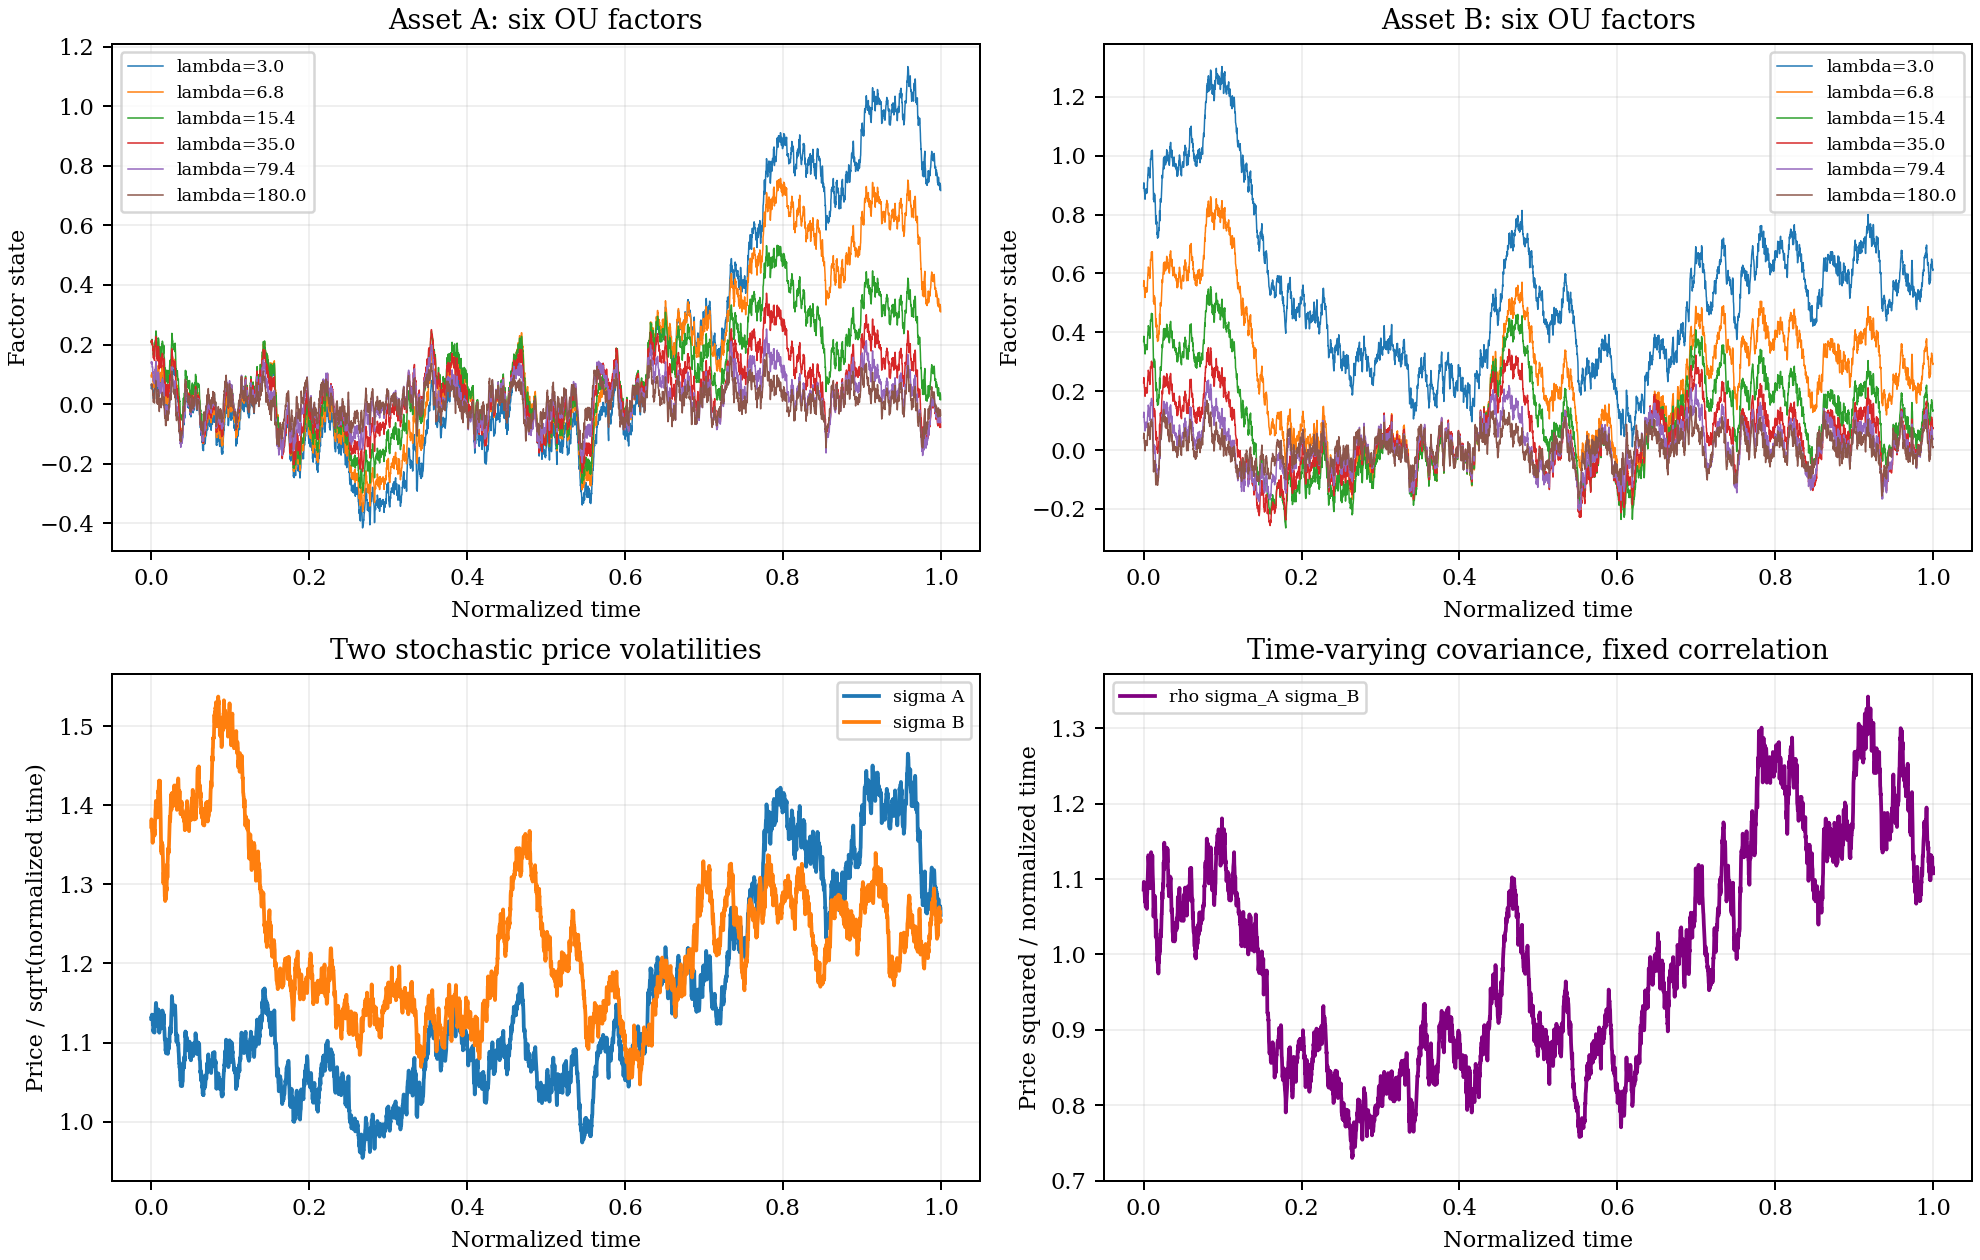
\includegraphics[width=\textwidth]{img/hft3-multiasset_volatility.png}
\caption{Two assets with six volatility factors each. Top panels show the two lifts; bottom panels show their distinct price volatilities and $\Sigma_{AB}=\rho\sigma_A\sigma_B$. Seed 73, path zero, stationary initial factor distribution, 3900 time intervals. Equal marginal parameters do not imply equal realized volatility paths.}
\label{hft3-fig:multi-vol}
\end{figure}

Exact innovations for the twelve-dimensional lift use
\[
 Q_{(i,m),(j,n)}=\nu_{ij}
 \frac{1-e^{-(\lambda_m+\lambda_n)\Delta t}}{\lambda_m+\lambda_n},
 \qquad \nu_{AA}=\nu_{BB}=1,\quad \nu_{AB}=0.35.
\]
The covariance is nearly singular for small steps. A spectral factorization removes only negative eigenvalues attributable to rounding, with a guard against a materially indefinite matrix. The maximum reconstruction discrepancy in the main run is $9.76\times10^{-19}$. This validates the factorization arithmetic, not the complete simulation discretization.

\subsection{How another asset's inventory changes a quote}
The variance rate of marked portfolio wealth is
\[
 \mathcal V(q,Y)=q^\top\Sigma(Y)q
 =q_A^2\sigma_A^2+q_B^2\sigma_B^2
 +2q_Aq_B\rho\sigma_A\sigma_B.
\]
With positive correlation, opposite-sign positions make the cross term negative. A short B position can therefore offset part of a long A exposure. The relevant object is this total risk, not the absolute inventory of either asset alone. For a unit sale of B, the exact change at fixed covariance is
\[
 \mathcal V(q-e_B,Y)-\mathcal V(q,Y)
 =-2(\Sigma q)_B+\Sigma_{BB}.
\]
Consequently the next sale reduces instantaneous risk only when $(\Sigma q)_B>\Sigma_{BB}/2$. The covariance benefit does not justify unlimited shorting. Finite order size, own-asset exposure, bounds and liquidation all matter. For example, at equal unit volatilities and $\rho=0.7$, moving from $(3,0)$ to $(3,-1)$ reduces the variance rate from 9 to 5.8; moving from $(3,-6)$ to $(3,-7)$ instead increases it, even before enforcing the inventory limit.

Multi-asset quoting and computational approximations are established research directions~\cite{BergaultEvangelistaGueantVieira2022,multifactor}. To isolate the mechanism with our existing numerical baseline, start from the separable value
\[
 \theta_{\rm sep}(t,q,Y)
 =\theta_0(t,q_A,Y_A)+\theta_0(t,q_B,Y_B).
\]
It ignores cross-asset inventory risk in its quote calculation. The first explicit correction is
\[
 C_{\rm cov}(t,q,Y)=-\gamma(T-t)\Sigma_{AB}(Y)q_Aq_B,
 \qquad \theta_{\rm cov}=\theta_{\rm sep}+C_{\rm cov}.
\]
This approximates the omitted integrated cross-risk by freezing the current covariance over the remaining horizon. It is not an exact expectation of future covariance, and it does not solve the joint control problem. It vanishes at $T$, preserving the separable terminal liquidation cost.

Define $s_B=\gamma(T-t)\Sigma_{AB}q_A$. Buying one unit of B changes the correction by $-s_B$, while selling one changes it by $+s_B$. Since the unbounded optimal offset equals the zero-gain offset minus the neighboring-inventory gain, the implementation adds $s_B$ to the raw bid offset and subtracts $s_B$ from the raw ask offset, then applies the declared bounds. Asset A uses the symmetric expression $s_A=\gamma(T-t)\Sigma_{AB}q_B$. Applying the correction before clipping avoids losing the original gain when the baseline control is already at a bound.

If $q_A>0$ and $\rho>0$, the B ask can therefore move downward relative to the separate policy: the dealer accepts a lower selling price because the fill can offset portfolio exposure. Its B bid also moves downward, discouraging further purchases. This is a change relative to the separate quote, not a promise to sell below the mid-price, nor a guaranteed execution. Figure~\ref{hft3-fig:multi-shift} makes the sign change with correlation and inventory visible while holding all other inputs fixed.

\begin{figure}[htbp]
\centering
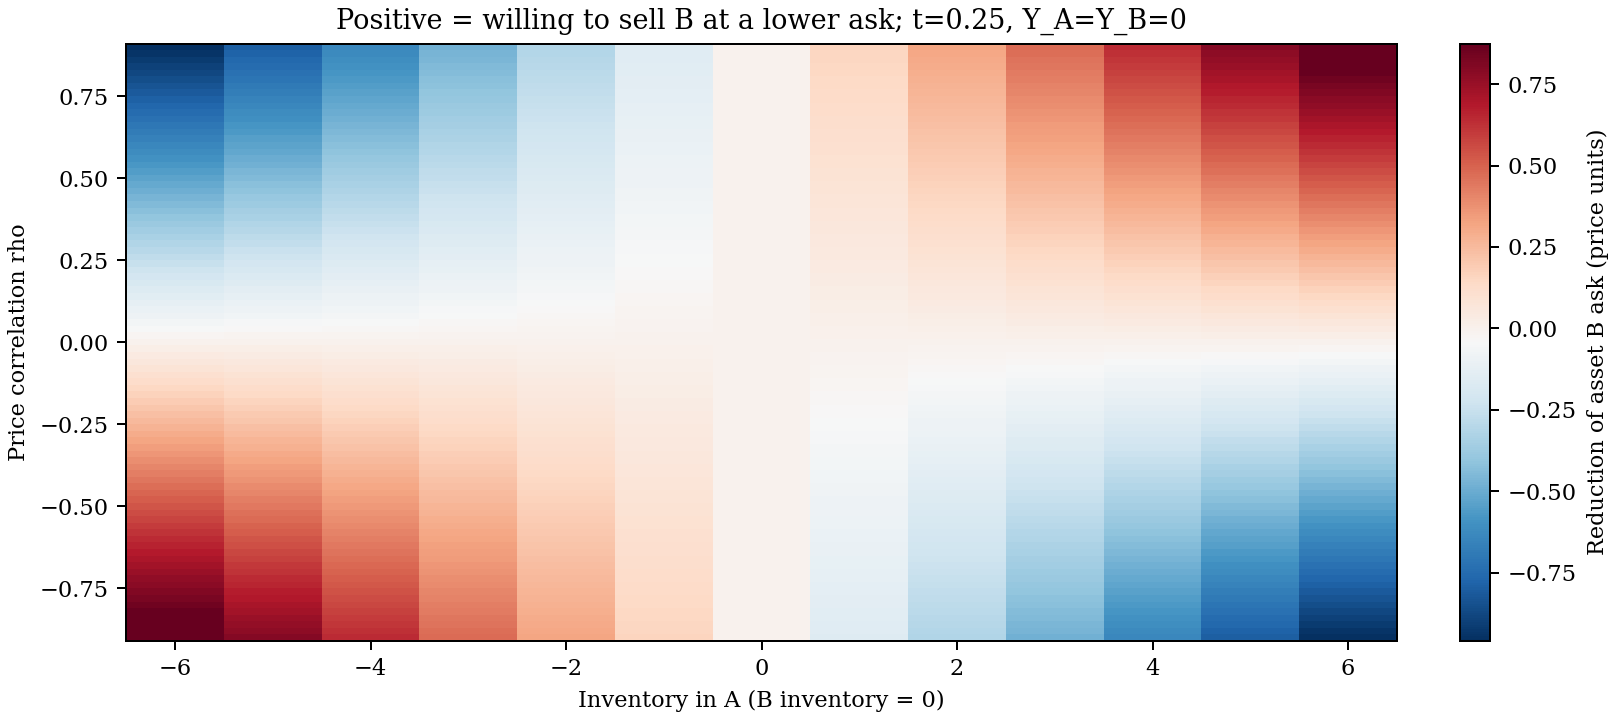
\includegraphics[width=\textwidth]{img/hft3-multiasset_quote_shift.png}
\caption{Reduction of asset B's ask relative to the separate policy, with $q_B=0$, $Y_A=Y_B=0$ and $t=0.25$. Positive values indicate a lower ask. The map varies price correlation and A inventory, using actual interpolated baseline gains and bounded controls. Zero correlation removes this explicit correction; negative correlation reverses its direction.}
\label{hft3-fig:multi-shift}
\end{figure}
\section{From a covariance proxy to a full residual correction}
The full lifted operator now has two inventory coordinates and twelve volatility coordinates. With $a$ the instantaneous covariance of the factor drivers and $\mathcal L_Z$ their OU generator, price/factor independence gives
\begin{align*}
\mathcal H[\theta]={}&\theta_t+\mathcal L_Z\theta
-\frac{\gamma}{2}(\nabla_Z\theta)^\top a\nabla_Z\theta
-\frac{\gamma}{2}q^\top\Sigma(Z)q\\
&+\sum_{i=1}^{2}\bigl[H_i(\theta(q+e_i)-\theta(q))
+H_i(\theta(q-e_i)-\theta(q))\bigr],
\end{align*}
omitting forbidden transitions. The C++ implementation supports fixed asset and total-factor dimensions and common arrival/control parameters; its caller supplies valid covariance matrices. Tests cover cross-asset risk, mixed factor Hessians, the gradient-square term and inventory bounds. In the restricted constant-covariance, no-arrival setting, the time derivative of $C_{\rm cov}$ exactly cancels the omitted cross-risk term relative to the diagonal baseline. That algebraic check does not establish cancellation in the stochastic-volatility model.

Indeed, $C_{\rm cov}$ also has factor derivatives when $\Sigma$ is stochastic, and changes all arrival Hamiltonians through the neighboring-inventory gains. Correlated volatility drivers introduce further mixed terms. The complete residual must be recomputed with these contributions before a localized fitted correction can be accepted. No residual reduction is asserted for the proxy in the experiment above.

For $N$ assets and $K$ total factors, a tensor inventory grid already contains $(2Q+1)^N$ states before discretizing volatility. Reusing separate scalar policies avoids that joint solve, but loses coupling. The explicit pair correction requires a covariance--inventory product, costing $O(N^2)$ for a dense covariance, in addition to scalar lookups; factor simulation costs are separate. This explains the proposed computational advantage and its approximation cost. No measured speedup is reported. A later fitted-policy study would require a validated multi-asset baseline and full residual to fit and test localized corrections, retaining risk, utility and computational cost as distinct acceptance criteria.
The equations now identify three errors to keep separate: approximation of memory by a finite lift, scalar compression within that lift, and numerical error in a chosen HJB solver. The numerical-methods chapter addresses the last one before the results test economic and residual effects.

\chapter{Numerical Methods and Implementation}\label{ch:numerics}
The same control logic needs two numerical layers: evolution or precomputation of a policy, and feedback simulation of executions. We describe their accounting conventions first, then the inherited solver's limitations, the positive bounded-control scheme and physical-time export. C++ is an implementation of these mathematical operators, not an independent model or a separate empirical result.
\section{Simulation and Experimental Design}


\subsection{The Time-Discretized Simulation Engine}
To numerically evaluate the strategies' performance, a custom simulation engine was implemented in Python. Contrary to a purely time-discretized approach, which would be analytically complex when coupling continuous diffusion processes (mid-price) with discrete jump processes (market orders), the simulator relies on an Euler-Maruyama discretization scheme.

The time horizon $T$ is partitioned into $N$ equidistant intervals of length $\Delta t$. At each discrete time step $t_i$, given the state vector comprising the mid-price $S_{t_i}$, the accumulated inventory $q_{t_i}$, and the cash account $X_{t_i}$, the simulator executes the following logical cycle.

\begin{enumerate}
    \item \textbf{Quote Generation:} The active policy computes the optimal quote prices $p^{bid}$ and $p^{ask}$ based on the current state, the remaining time to horizon $\tau$, and the risk aversion parameter $\gamma$.
    \item \textbf{Probability Evaluation:} The theoretical Poisson intensities $\lambda^{bid}$ and $\lambda^{ask}$ are mapped into discrete transition probabilities for the interval $\Delta t$, defined as
    \begin{align*}
        p_{fill} = 1 - e^{-\lambda \Delta t}.
    \end{align*}
    \item \textbf{Execution Matching:} Two independent uniform random variables, $U^{bid}_{t_i}, U^{ask}_{t_i} \sim \mathcal{U}(0,1)$, are compared with the respective fill probabilities. If $U < p_{fill}$, the order is considered executed. In this implementation, each side can have at most one unit fill per time step and the rule is therefore a Bernoulli discretization of the underlying Poisson arrival process.
    \item \textbf{State Update:} In the event of a bid execution, inventory increases ($q_{t_{i+1}} = q_{t_i} + 1$) and the cash account decreases by the bid price ($X_{t_{i+1}} = X_{t_i} - p^{bid}$). Conversely, an execution at the ask reduces inventory and increases cash.
    \item \textbf{Mark-to-Market:} Performance is recorded by updating the total wealth (PnL), defined as
    \begin{align*}
        W_{t_{i+1}} = X_{t_{i+1}} + q_{t_{i+1}} S_{t_{i+1}}.
    \end{align*}
\end{enumerate}

\subsection{Experimental Control: Common Random Numbers (CRN)}
To rigorously isolate the performance differential between the symmetric benchmark and the inventory-aware policies, the experimental design employs the variance reduction technique known as Common Random Numbers (CRN).

In the Monte Carlo probability space, the entire stochastic scenario is pre-calculated via vectorized matrices. For each $m$-th simulated trajectory, a single master seed generates, at first, the sequence of Brownian increments ($\Delta W^{(m)}$) driving the mid-price process. Then the uniform random variables ($U^{bid, (m)}, U^{ask, (m)}$) governing order execution at each tick.

Both the Naive dealer and the Avellaneda--Stoikov dealer are tested on the exact same scenario. By subjecting the algorithms to the same price shocks and client order flows, the experimental design eliminates inter-path stochastic noise. Any observed disparity in terminal wealth or inventory accumulation is therefore solely attributable to the internal risk-management logic of the respective algorithms.

\subsection{Performance Metrics}
The simulator tracks the state variables to extract terminal distributions. Terminal wealth $W_T$ is reported on a mark-to-market basis, i.e., it includes the cash account plus the value of any remaining inventory at the terminal mid-price; no separate forced liquidation trade or liquidation cost is applied. The comparative analysis is based on the following key metrics:

\begin{itemize}
    \item Expected Terminal Wealth ($\mathbb{E}[W_T]$): the average profit generated across all Monte Carlo paths, representing the pure spread-capture capability.
    \item Wealth Variance ($Var(W_T)$): the dispersion of terminal PnL, acting as the primary proxy for unmanaged inventory and price risk.
    \item Sharpe-like ratio: calculated as the ratio between average terminal PnL and its standard deviation across Monte Carlo paths. It is an internal simulation diagnostic, not an annualized market Sharpe ratio.
    \item Expected Absolute Terminal Inventory ($\mathbb{E}[|q_T|]$): the average magnitude of the open position remaining at the end of the trading horizon $T$. This metric quantifies the strategy's capacity for mean-reversion, measuring how effectively it avoids overnight directional exposure.
    \item Inventory Dispersion ($\mathbb{E}[Std(q_t)]$): the average standard deviation of the inventory throughout the trading session. This metric captures the intraday risk profile, distinguishing between a strategy that tightly bounds its position (capital efficiency) and one that suffers large directional swings, regardless of the final terminal state.
    \item Expected Turnover ($\mathbb{E}[\text{Turnover}]$): the average volume of executed trades per simulation, serving as a proxy for the strategy's operational efficiency and its potential vulnerability to unmodeled transaction costs.
\end{itemize}

The analysis does not rely on the calibration of real historical data but rather on the definition of stylized scenarios. This approach allows for systematic stress-testing of the models in controlled regimes (varying volatility $\sigma$ and book density $k$), ensuring maximum reproducibility and isolating the structural mechanisms of the Avellaneda--Stoikov framework without the biases inherent to specific market datasets.





\subsection{Figure Construction Algorithms}
The numerical figures are produced from the same simulation objects used to compute the tables. To avoid repeating the same methodological explanation below each figure, we report the plotting logic once here as part of the simulation design. Panels (a)--(d) in the single-asset ABM and GBM figures follow the four algorithms below: mid-price and quotes, inventory path, mark-to-market PnL, and Monte Carlo terminal PnL distribution. In the multivariate figure, however, the first mid-price-and-quotes panel is intentionally not reported: we did not produce the multivariate mid-price-and-quotes graph because, with three assets, plotting all mid-prices together with their bid and ask quotes would make the panel unreadable. For this reason, panel (a) of the multivariate figure is replaced by cumulative log-returns, while panels (b)--(d) preserve the same portfolio-risk, PnL, and terminal-distribution logic.

\begin{algorithm}[H]
\caption{Panel (a): Mid-price and quotes}
\DontPrintSemicolon
\KwIn{Time grid $(t_i)_{i=0}^{n}$, simulated mid-price path $(S_{t_i})$, quoted bid and ask arrays for the naive and AS strategies.}
\KwOut{A price panel comparing the reference mid-price with the two quoting rules.}
Plot the mid-price path $S_{t_i}$ as the common reference line\;
Plot the naive bid and ask quotes $p_{t_i}^{bid,N}$ and $p_{t_i}^{ask,N}$ around $S_{t_i}$\;
Plot the AS bid and ask quotes $p_{t_i}^{bid,AS}$ and $p_{t_i}^{ask,AS}$ around the inventory-adjusted reservation price\;
Use the panel to visualize the quote skew: the naive quotes remain symmetric around $S_t$, while the AS quotes move with inventory through $r_t$\;
\end{algorithm}

\begin{algorithm}[H]
\caption{Panel (b): Inventory path}
\DontPrintSemicolon
\KwIn{Time grid $(t_i)_{i=0}^{n}$ and inventory paths $(q_{t_i}^{N})$, $(q_{t_i}^{AS})$.}
\KwOut{A pathwise comparison of inventory accumulation and mean-reversion.}
For each strategy, update inventory after bid and ask fills according to $dq_t=dN_t^{bid}-dN_t^{ask}$\;
Plot the naive inventory path $q_{t_i}^{N}$ and the AS inventory path $q_{t_i}^{AS}$\;
Add the zero-inventory line as the natural benchmark\;
Use the panel to evaluate whether the quoting rule creates an endogenous pull back toward $q_t=0$\;
\end{algorithm}

\begin{algorithm}[H]
\caption{Panel (c): Mark-to-market PnL}
\DontPrintSemicolon
\KwIn{Cash paths $(X_{t_i}^{N})$, $(X_{t_i}^{AS})$, inventories $(q_{t_i}^{N})$, $(q_{t_i}^{AS})$, and price path $(S_{t_i})$.}
\KwOut{A realized path of mark-to-market wealth for both strategies.}
At each time step, compute realized wealth as $W_{t_i}=X_{t_i}+q_{t_i}S_{t_i}$ in the single-asset case\;
For the multivariate case, compute $W_{t_i}=X_{t_i}+q_{t_i}^{\top}S_{t_i}$\;
Plot the naive and AS wealth paths on the same axes\;
Interpret the panel only as one realized scenario, not as the final statistical comparison\;
\end{algorithm}

\begin{algorithm}[H]
\caption{Panel (d): Terminal PnL distribution}
\DontPrintSemicolon
\KwIn{Monte Carlo samples of terminal wealth $\{W_T^{N,(m)}\}_{m=1}^{M}$ and $\{W_T^{AS,(m)}\}_{m=1}^{M}$.}
\KwOut{A density histogram comparing terminal PnL dispersion across strategies.}
Run both strategies on the same simulated price paths and fill uniforms using common random numbers\;
Collect terminal mark-to-market PnL $W_T^{(m)}$ for each Monte Carlo path $m=1,\ldots,M$\;
Build normalized histograms using the same bins for the naive and AS samples\;
Add vertical lines at the sample means of the two terminal PnL distributions\;
Use the panel to compare dispersion and tail exposure, not only average terminal PnL\;
\end{algorithm}

With the simulation architecture fixed, the remaining task is empirical comparison within the stylized Monte Carlo environment. The results chapter combines the diffusion diagnostics with the finite-lift and positive-baseline experiments under their separate accounting conventions.
\section{Inherited scalar audit and positive bounded baseline}


The audit imports the inspected HFT2 source without modifying it and runs its default scalar solver for $H=0.2$. Synthetic stationary lifted states are sampled with seed 42. Evaluation uses time indices $0$, $195$ and $388$, five inventory levels and twelve states per combination, producing 180 interior samples. Time differentiation is forward, spatial differences follow the inherited solver and derivative values are linearly interpolated.

\begin{center}
\begin{tabular}{@{}lr@{}}
\toprule
Diagnostic & Value \\
\midrule
Full aggregate instantaneous variance & $1.000000$ \\
Reduced diffusion variance & $0.209552$ \\
Full residual RMS & $138562.58$ \\
Reduced residual RMS & $113726.58$ \\
Operator-difference RMS & $38015.32$ \\
Pre-terminal entries at lower clip $-60$ & $6514$ \\
Pre-terminal entries at upper clip $15$ & $159144$ \\
\bottomrule
\end{tabular}
\end{center}

These unnormalized values are diagnostics under the declared discretization and bounded Hamiltonian. The inherited solver clips its value array and uses a different, unconstrained arrival term. Both choices matter when interpreting the residual. Entries at clipping bounds do not by themselves identify the cause of the numerical behavior, but the combination of extensive saturation and a large reduced residual rules out treating this run as a validated converged baseline. Its RMS magnitudes must not be directly ranked against the later positive-baseline off-grid diagnostic: sample sets, derivative reconstruction and numerical surfaces differ.

An independent C++ evaluation agrees with the exported Python residuals on all 180 samples within the prescribed relative tolerance $10^{-9}(1+|R|)$. The deterministic test executable passes 528 checks. These results verify implemented arithmetic and selected interfaces; they do not validate an optimal policy or justify a correction fit on the saturated baseline.

\section{A positive transformed baseline}
To address this issue, the next implementation uses $u=\exp(-\gamma\theta)>0$. On the scalar state grid its equation is
\begin{align*}
0={}&u_t+\mathcal L_Ru+\tfrac12\gamma^2q^2v(y)u\\
 &+\sum_{\pm}\min_{\delta\in[0.02,4]}
 Ae^{-k\delta}\bigl(e^{-\gamma\delta}u_{q\pm1}-u_q\bigr),
\end{align*}
where forbidden inventory transitions are omitted. The terminal condition is $u(T,q,y)=\exp(\gamma L(q,y))$. The transformation removes the spatial gradient-square term; it does not remove the coupled control optimization over neighboring inventories.

For spacing $h$, use nonnegative state-transition rates
\[
 a_-={\eta^2\over2h^2}+{\max(-b,0)\over h},\qquad
 a_+={\eta^2\over2h^2}+{\max(b,0)\over h},\qquad b=-\kappa y.
\]
Outward state transitions are suppressed at the two truncated boundaries. Each backward explicit step uses the minimizing quotes computed from the current positive array. The condition
\[
 \Delta t\left(a_-+a_++2Ae^{-k\delta_{\min}}\right)<1
\]
is sufficient for nonnegative coefficients in each controlled step; the inventory-risk term adds a nonnegative diagonal contribution. This gives an algebraic positivity property of the scheme. It is not a proof of convergence to the unbounded-domain HJB. Domain truncation, consistency, time error and policy error still require study.

The implementation chooses substeps from a conservative global bound with safety factor $0.8$. It reports a failure if a transformed value becomes nonpositive or nonfinite; no clipping of $\theta$ is used. Deterministic tests pass for a constant solution, an analytic no-arrival constant-volatility limit, inventory symmetry, positivity and invalid grids.

\begin{center}
\begin{tabular}{@{}rrrr@{}}
\toprule
State points & Time steps & $\theta(0,0,0)$ & $\theta(0,2,0)$\\
\midrule
61 & 2340 & 6.701053 & 6.367267\\
61 & 4680 & 6.699587 & 6.365723\\
121 & 2340 & 6.701135 & 6.367370\\
121 & 4680 & 6.699669 & 6.365826\\
241 & 2340 & 6.701176 & 6.367421\\
241 & 4680 & 6.699709 & 6.365878\\
\bottomrule
\end{tabular}
\end{center}
All six runs keep $u$ positive. With 4680 time steps, the change in $\theta(0,0,0)$ from 121 to 241 points is approximately $4.08\times10^{-5}$; halving the time step at 241 points changes it by approximately $1.47\times10^{-3}$. These are selected-point refinement diagnostics, not global error bounds. These initial runs exported only time-zero values. The following experiment extends the export to physical-time slices and examines joint domain/grid sensitivity; independent residual validation remains open.

\section{Time-dependent policies and domain sensitivity}
The next increment retains 41 physical-time slices, including both endpoints, from each backward solve. Nine configurations combine 81, 161 and 241 state nodes with symmetric domains of four, five and six stationary standard deviations. All use 9360 actual time steps. These are discretizations of the same scalar model, not nine market models or simulated trading sessions. The CSV export contains 772317 state-time-inventory records. An unavailable quoting side at an inventory limit is stored as missing, not as a zero offset.

Figure~\ref{hft3-fig:temporal-policy} shows the solved baseline at three times. The rows expose the approach to the liquidation condition; the columns distinguish the certainty equivalent from executable offsets. Inventory is discrete, so horizontal bands are expected. White boundary rows mark forbidden trades. The color scales are local to each panel. Near the terminal time, aggressive offsets can reach the declared lower bound; this is a control constraint, not clipping of the value function.

\begin{figure}[p]
\centering
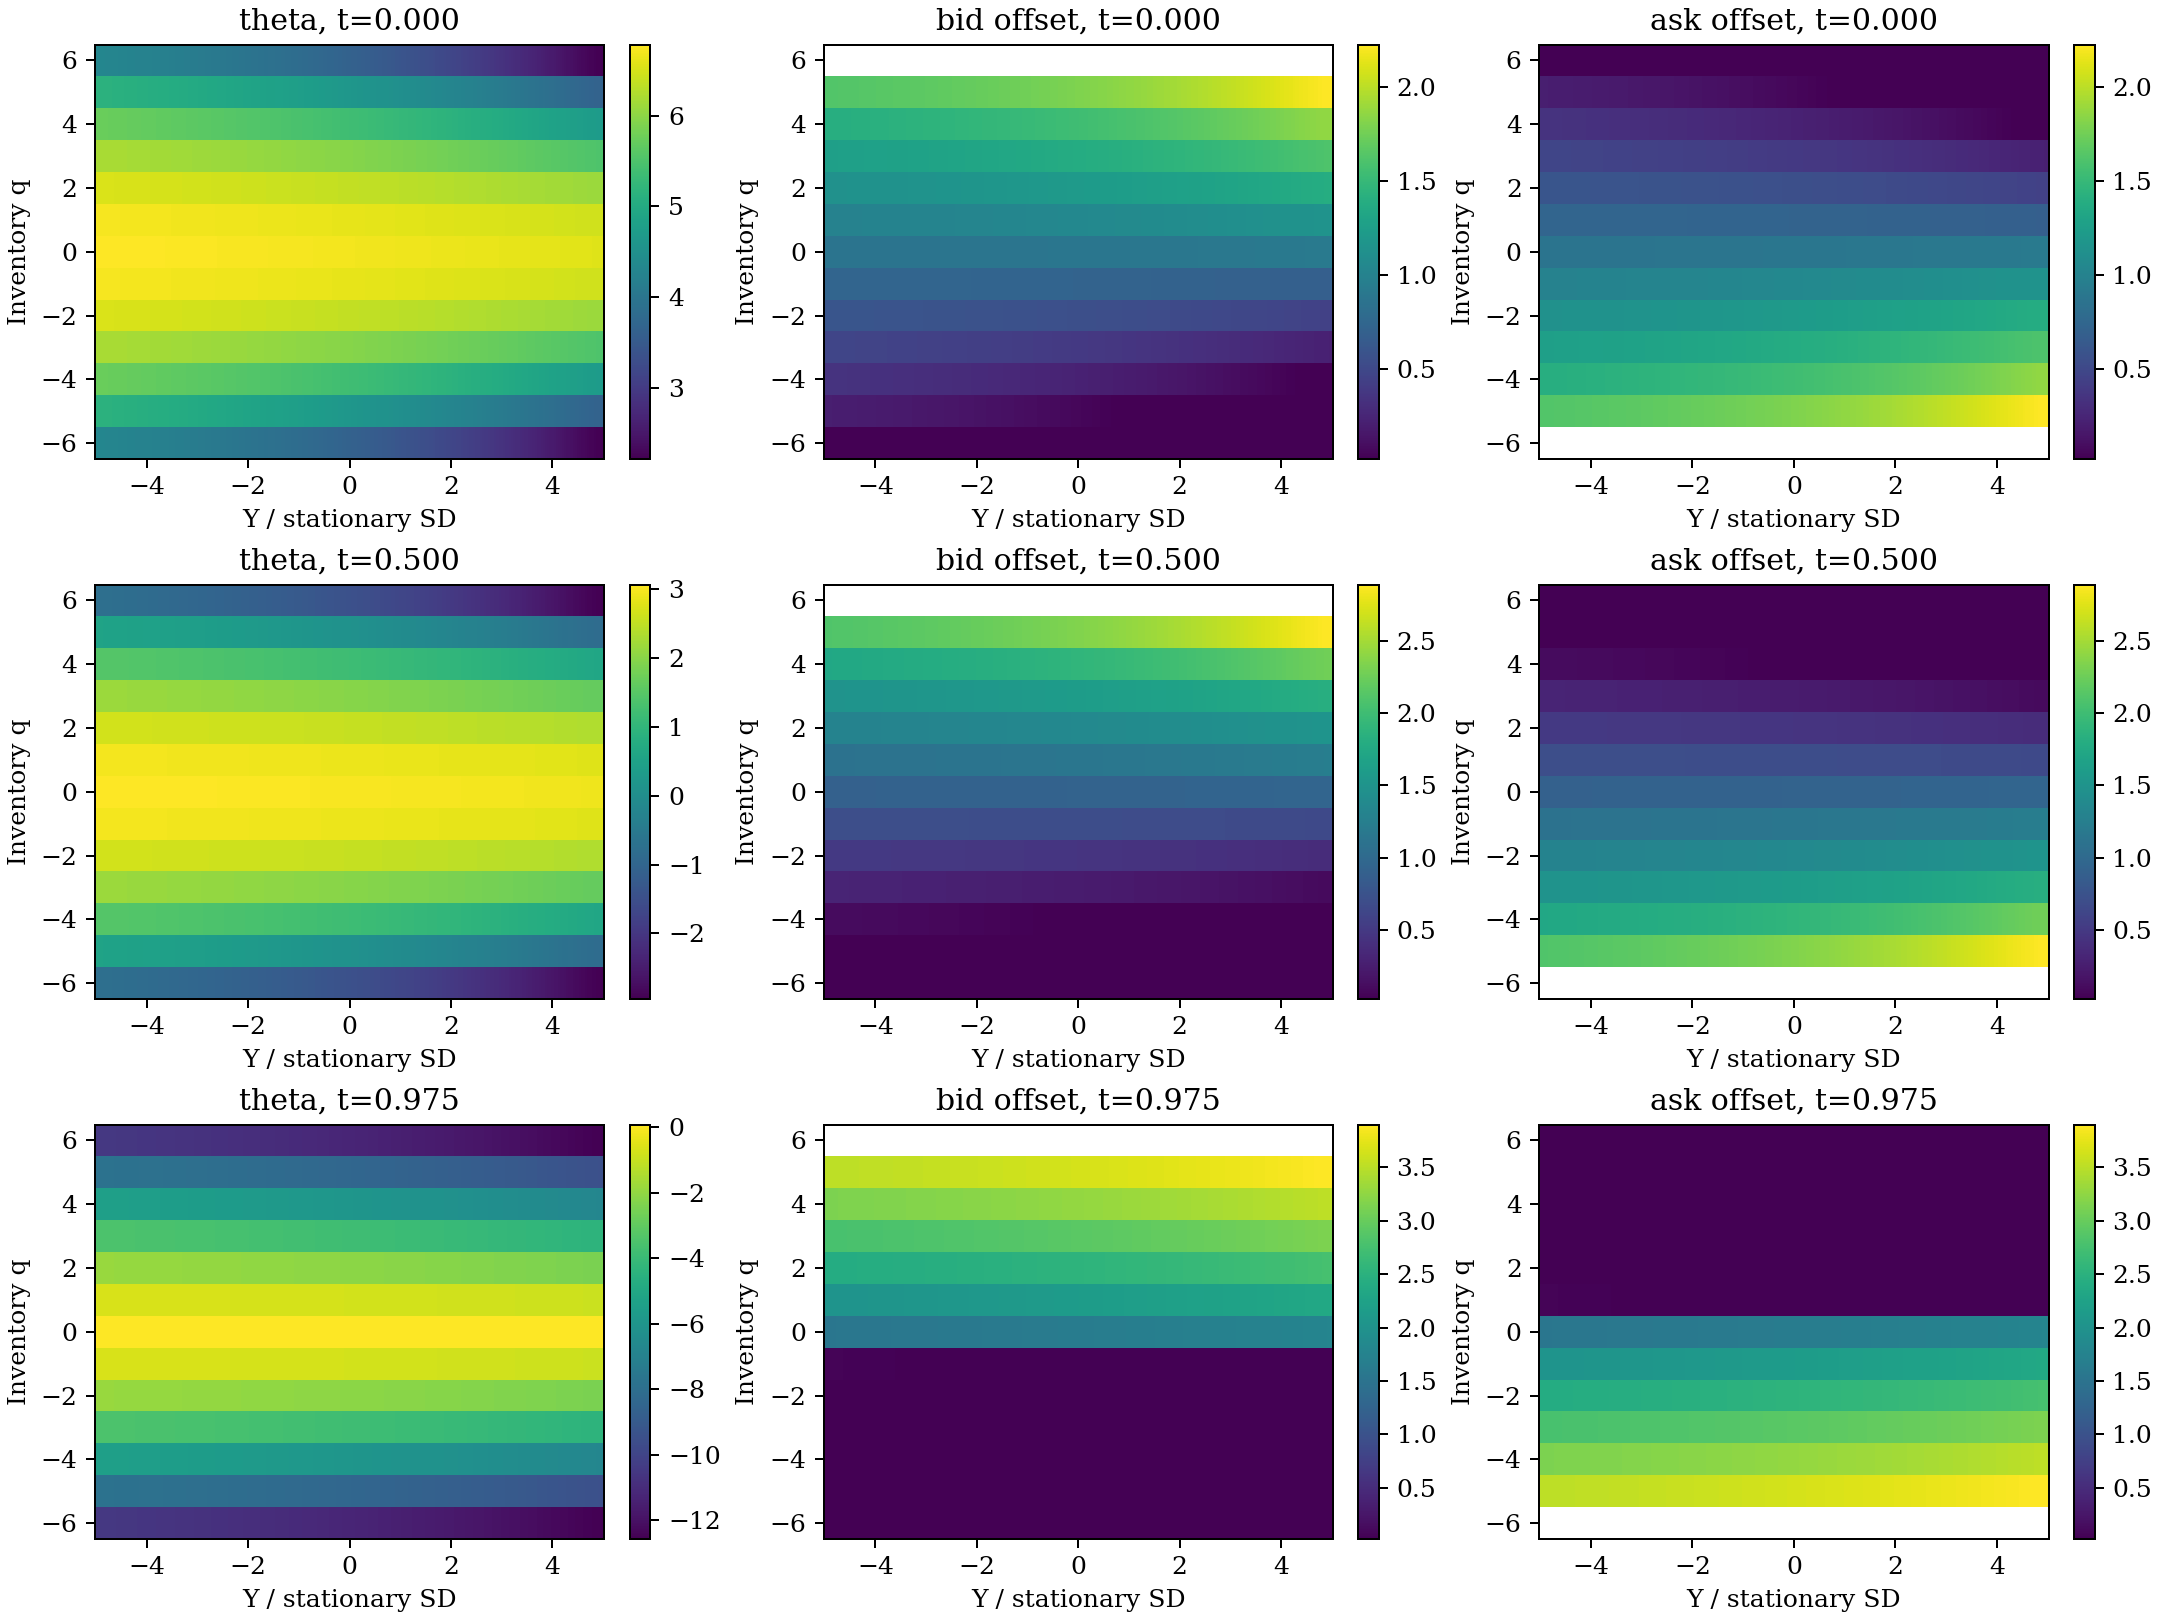
\includegraphics[width=\textwidth]{img/hft3-temporal_policy.png}
\caption{Solved scalar baseline: certainty equivalent and bid/ask offsets at $t=0$, $0.5$ and $0.975$, with $T=1$. Domain $\pm5$ stationary standard deviations, 241 state nodes, 9360 steps. Values and offsets use the model's monetary/price units; time is normalized. Blank cells denote disabled sides at inventory limits. Deterministic HJB computation, not Monte Carlo.}
\label{hft3-fig:temporal-policy}
\end{figure}

The export checks recover the terminal condition with maximum absolute error $5.33\times10^{-15}$, and all available offsets remain in $[0.02,4]$. Additional C++ tests verify temporal ordering, endpoint inclusion, the analytic no-arrival risk limit at every saved time, and exact agreement between the final snapshot and the existing time-zero API. Exporting the history does not change the numerical evolution.

Figure~\ref{hft3-fig:policy-sensitivity} compares all saved times, inventory levels and admissible sides on 101 common points in $|Y|\leq2\sqrt{\operatorname{Var}(Y)}$. Linear interpolation maps each grid to these points. The six-standard-deviation, 241-node run is a comparison surface, not an exact solution. Across the configurations, maximum differences are approximately $1.62\times10^{-3}$ for the value and $1.15\times10^{-3}$ for offsets. The zero at the reference configuration is an identity, not evidence of zero numerical error.

\begin{figure}[htbp]
\centering
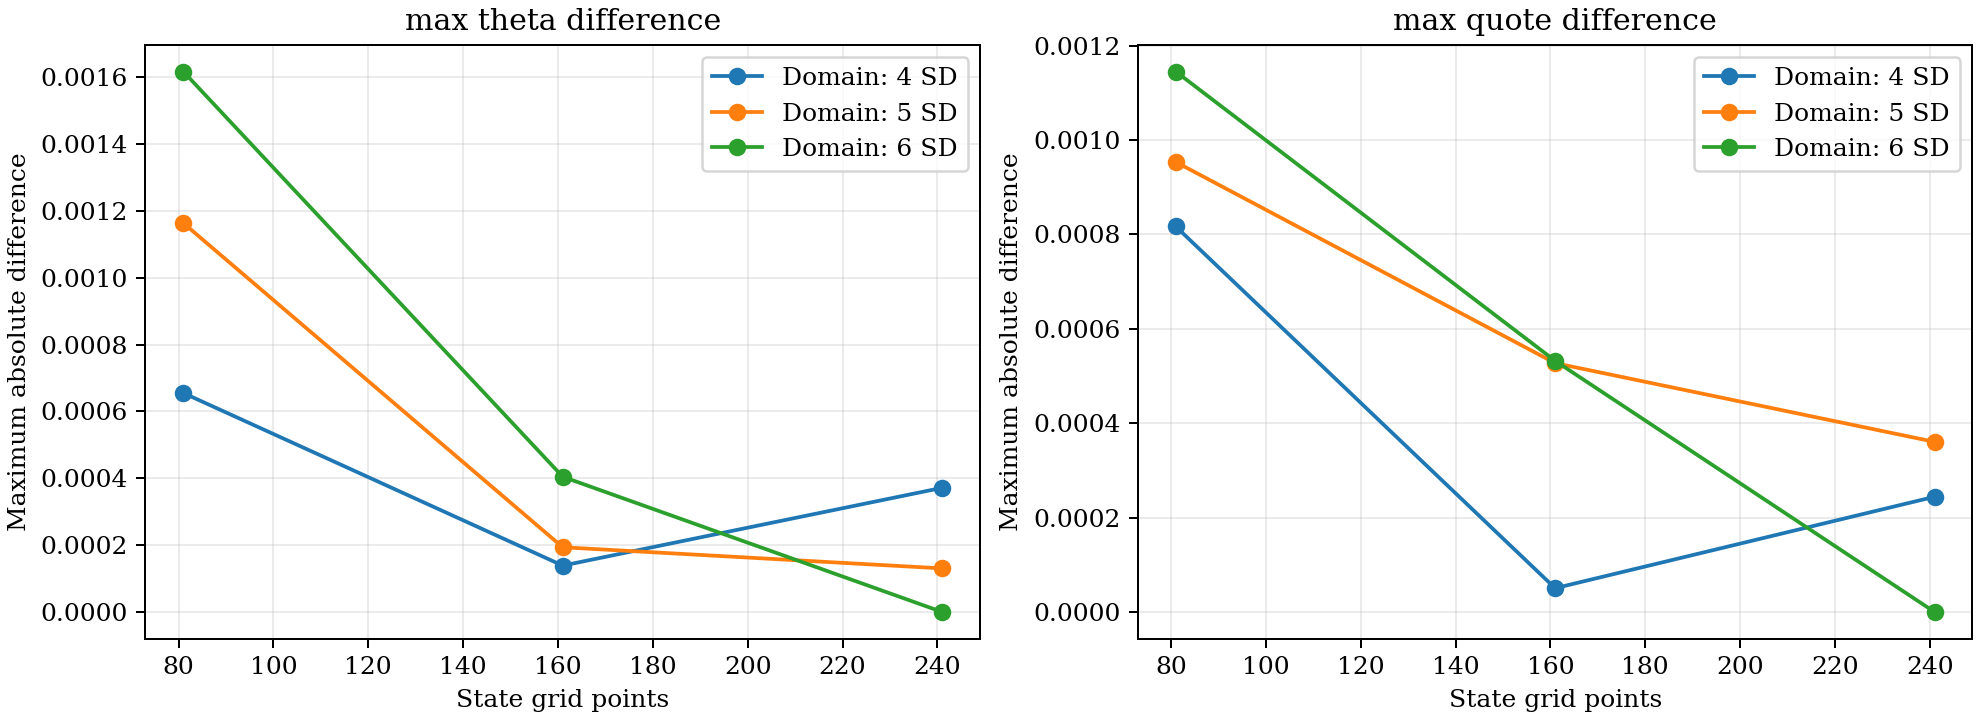
\includegraphics[width=\textwidth]{img/hft3-policy_sensitivity.png}
\caption{Joint grid/domain sensitivity relative to the six-standard-deviation, 241-node run, at a common 9360 time steps. Maxima cover all 41 saved times and the central two-standard-deviation interval. Changing the domain at fixed node count also changes spacing; the nonmonotone four-standard-deviation curve cannot be interpreted as an isolated boundary error.}
\label{hft3-fig:policy-sensitivity}
\end{figure}

The computational purpose of precomputation is to move HJB evolution outside the decision loop. Saving selected slices costs memory proportional to the number of stored times, inventory levels and state nodes, rather than requiring every solver step to be retained. This increment supplies offline CSV data; interpolation refinement and a measured speed advantage remain pending. The separate temporal and fixed-spacing studies reported in the comparative-results chapter extend these joint sensitivities; independent derivative/residual convergence remains a gate before fitting corrections. In particular, the figures do not yet establish full-state accuracy or economic performance.

\clearpage
\section{C++ operators and offline policy export}


The implemented offline path evaluates the full operator and exports baseline policy surfaces; fitting corrections remains a proposed extension. The online target is a fixed-size factor update, aggregation, baseline lookup, gate evaluation and a small bounded number of correction lookups. The state recurrence alone costs $O(M)$. Exact correlated OU innovation generation with a dense precomputed factor costs $O(M^2)$ per simulation step; its factorization costs $O(M^3)$ offline. Correction cost also includes feature construction and support selection. These components must be timed separately before assigning a complexity or latency to the complete decision. The offline Hessian contraction currently costs $O(M^2)$; it is not part of the online latency claim.

The first implementation provides a bounded arrival Hamiltonian, a common-noise full residual evaluator, scalar-to-vector derivative embedding, a smooth gate and exact correction-product derivatives. Parameters and diagnostic inputs are validated. Arithmetic overflow in the residual is reported instead of silently clipping it. Tests cover inventory limits, quote optimization against a grid search, mixed Hessian terms, scalar embedding, gate derivatives and nonlinear recomputation.

The archived original demonstration used synthetic surfaces without a time coordinate. A finite-horizon solved policy must represent the remaining time explicitly or use an equivalent validated selection of time slices. It would be misleading to report the starter's lookup as the performance of the future corrected HJB policy.

Software timing will be measured separately for factor updates, baseline lookups, corrections and the complete decision. Warm-up, timer overhead, repeated trials, compiler flags and hardware disclosure are prerequisites. No exchange round-trip claim follows from a local microbenchmark. The comparative-results chapter reports the checks and experiments completed under these conventions.

The comparative-results chapter now applies these conventions to the diffusion models, memory-inspired finite lifts and covariance proxy. The mathematical form of a quote is shared, but terminal accounting, approximation level and numerical resolution are stated separately for each experiment.

\chapter{Comparative Evidence Across Model Classes}\label{ch:results}
The models can now be compared through a common set of questions: what happens to execution revenue, inventory exposure, terminal liquidation and the control equation? Comparisons are paired within a declared experiment. Absolute PnL across rows is not a common score: terminal costs, control bounds, initialization and simulation designs differ. The diffusion benchmark uses terminal marked wealth, while the liquidation experiments deduct a declared close-out cost once.

\section{Markovian diffusion benchmarks}



\subsection{Single-Asset Monte Carlo Diagnostics}

The single-asset experiment uses $N=5{,}000$ Monte Carlo paths, $T=1$, $1{,}000$ time steps, $S_0=100$, $\gamma=0.1$, $k=1.5$, $A=140$, and the optimal liquidity half-spread
\[
\delta^*=
\frac{1}{\gamma}\log\!\left(1+\frac{\gamma}{k}\right)
=
0.6454.
\]
The ABM volatility is $\sigma_{ABM}=1.5$. The GBM volatility is calibrated as $\sigma_{GBM}=0.015$, so that $\sigma_{GBM}S_0=\sigma_{ABM}$ and both models have the same initial dollar volatility.

\begin{table}[H]
\centering
\small
\caption{Single-asset Monte Carlo diagnostics with $5{,}000$ simulated paths and inventory-based improvement relative to naive quoting. Negative values in inventory and volatility metrics indicate risk reduction.}
\begin{tabular*}{\textwidth}{@{\extracolsep{\fill}}l!{\vrule width 0.5pt}rrr!{\vrule width 0.5pt}rrr@{}}
\toprule
Metric & ABM Naive & ABM AS & Difference & GBM Naive & GBM AS & Difference \\
\midrule
Mean terminal PnL        & 67.145 & 63.930 & -3.215 & 67.109 & 63.894 & -3.215 \\
Std terminal PnL         & 12.178 &  6.680 & -5.498 & 12.316 &  6.718 & -5.598 \\
Sharpe-like ratio        &  5.514 &  9.570 &  4.056 &  5.449 &  9.511 &  4.062 \\
Mean $|$terminal inv$|$  &  7.817 &  3.116 & -4.701 &  7.897 &  3.095 & -4.802 \\
Mean Std$(q_t)$          &  3.708 &  1.799 & -1.909 &  3.727 &  1.795 & -1.932 \\
Mean turnover            &103.845 &107.414 &  3.569 &103.618 &107.298 &  3.680 \\
\bottomrule
\end{tabular*}
\end{table}

The central result is not that the inventory-based dealer always maximizes raw terminal PnL path by path. In the ABM and GBM Monte Carlo tables, the naive dealer has a slightly higher average terminal PnL, roughly $3.2$ units more in both models. This is expected in a simplified simulator without adverse selection, market impact, fees, or hard inventory limits: a symmetric dealer can sometimes earn more gross spread by accepting larger inventory risk.

The relevant advantage of the Avellaneda--Stoikov rule is risk adjustment. Under ABM, the standard deviation of terminal PnL falls from $12.178$ to $6.680$, while the Sharpe-like ratio rises from $5.514$ to $9.570$. The mean absolute terminal inventory falls from $7.817$ to $3.116$, and the average intraday inventory standard deviation is almost halved. The GBM case produces the same qualitative pattern: lower PnL dispersion, lower terminal inventory, lower intraday inventory variability, and a much higher Sharpe-like ratio. The slight increase in turnover is consistent with the mechanism of the strategy: the AS dealer actively skews quotes to encourage inventory-reducing trades.

\begin{figure}[H]
\centering
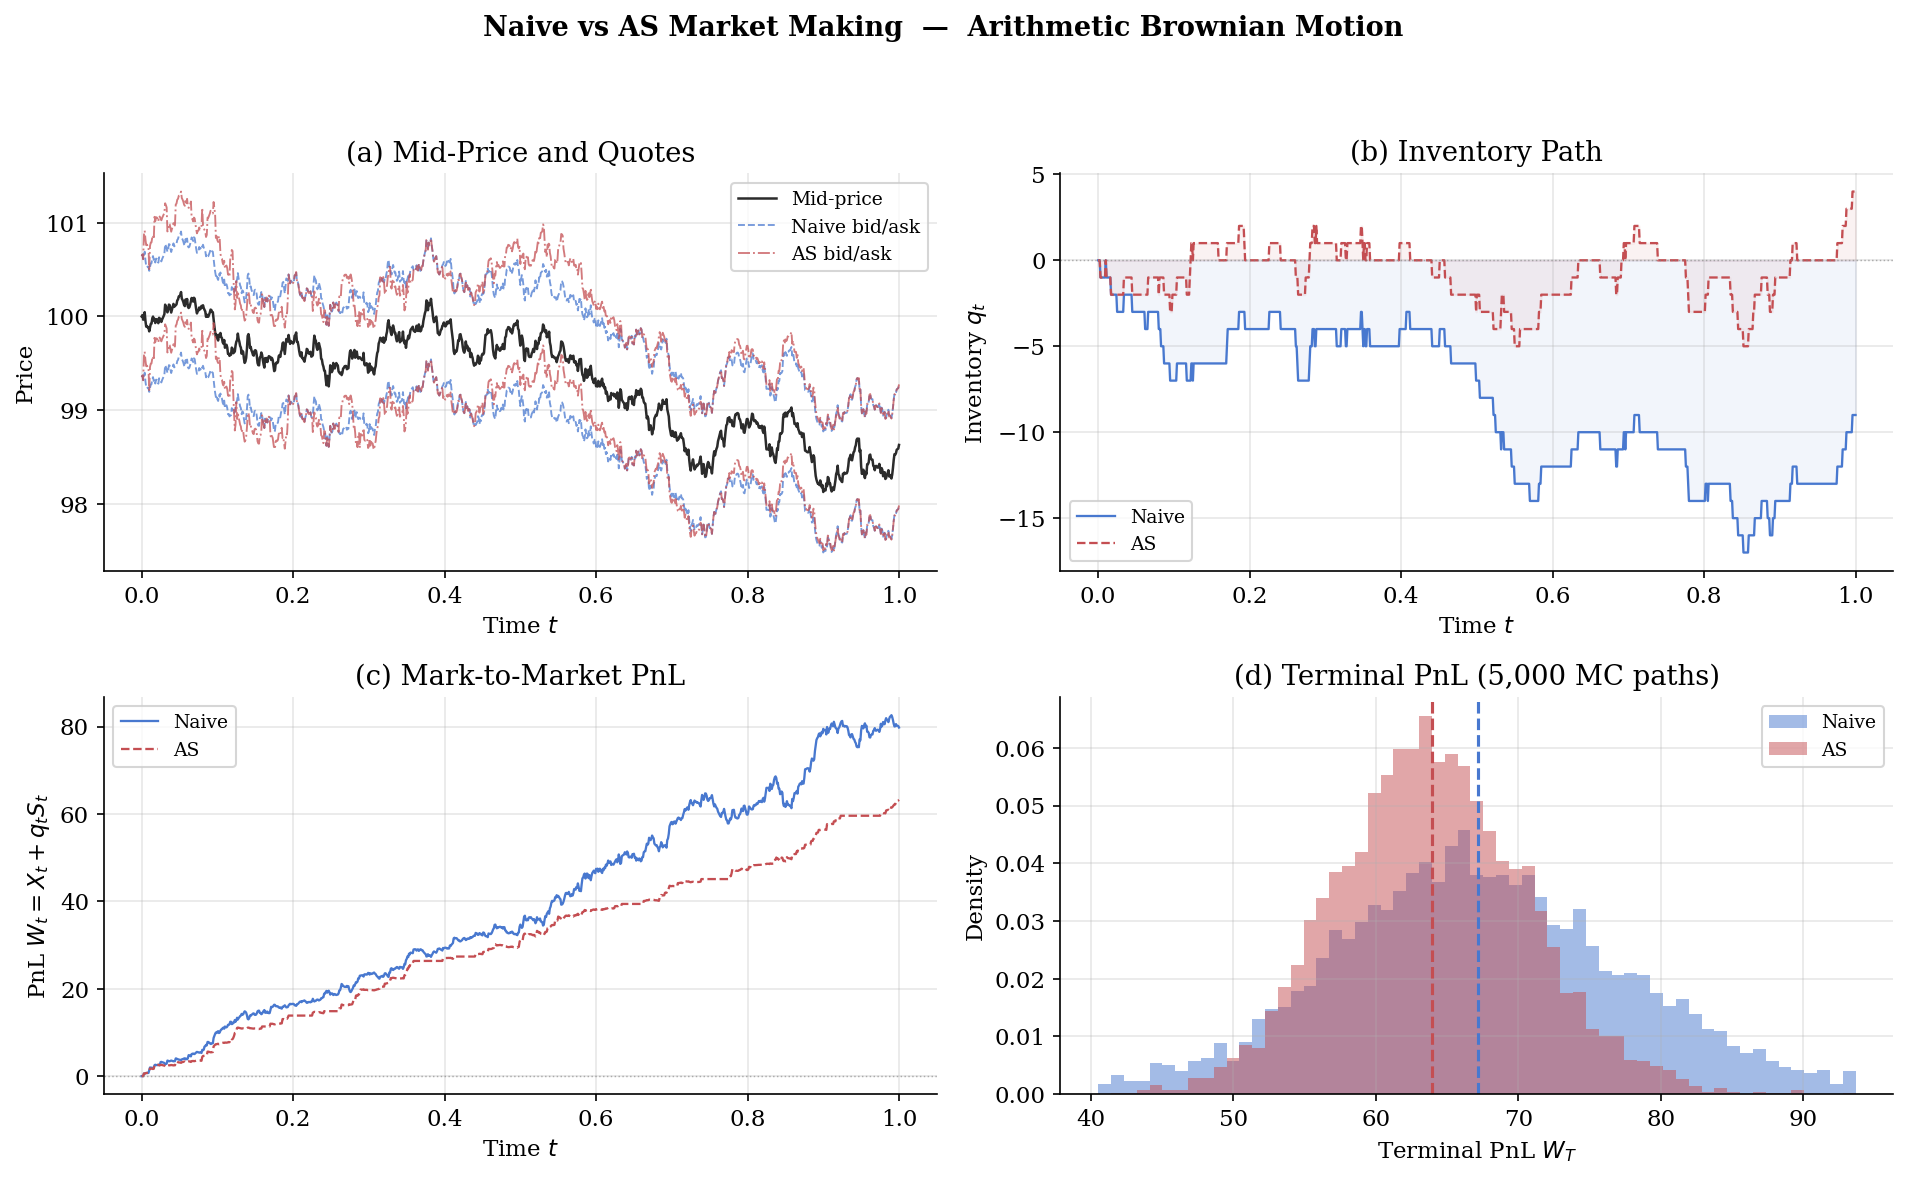
\includegraphics[width=0.85\textwidth]{img/hft1-py1.png}
\caption{Single-asset ABM comparison: naive versus Avellaneda--Stoikov quoting.}
\label{hft1-fig:bm_results}
\end{figure}

Figure~\ref{hft1-fig:bm_results} illustrates the ABM case. Panel (a) shows that both strategies quote around the same mid-price, but the AS quotes are not fixed symmetrically around $S_t$: they move with inventory through the reservation-price adjustment. When the dealer accumulates a long inventory, the quote center is pushed downward to make selling more likely and further buying less attractive; when the dealer is short, the opposite adjustment occurs. Panel (b) makes this mechanism visible. The naive inventory drifts much further from zero because the policy has no endogenous force pulling $q_t$ back toward neutrality, while the AS inventory is actively stabilized by the quote skew. Panel (c) should be read as a single realized path, not as the main performance criterion. In this particular path, the naive strategy ends higher because the realized price movement happens to reward the inventory exposure it has accumulated. Panel (d) is therefore the more relevant diagnostic: over $5{,}000$ paths, the naive terminal PnL distribution is wider, whereas the AS distribution is more concentrated. The message is that the AS rule does not simply try to maximize one lucky path; it reduces the dispersion generated by unmanaged inventory exposure.

\begin{figure}[H]
\centering
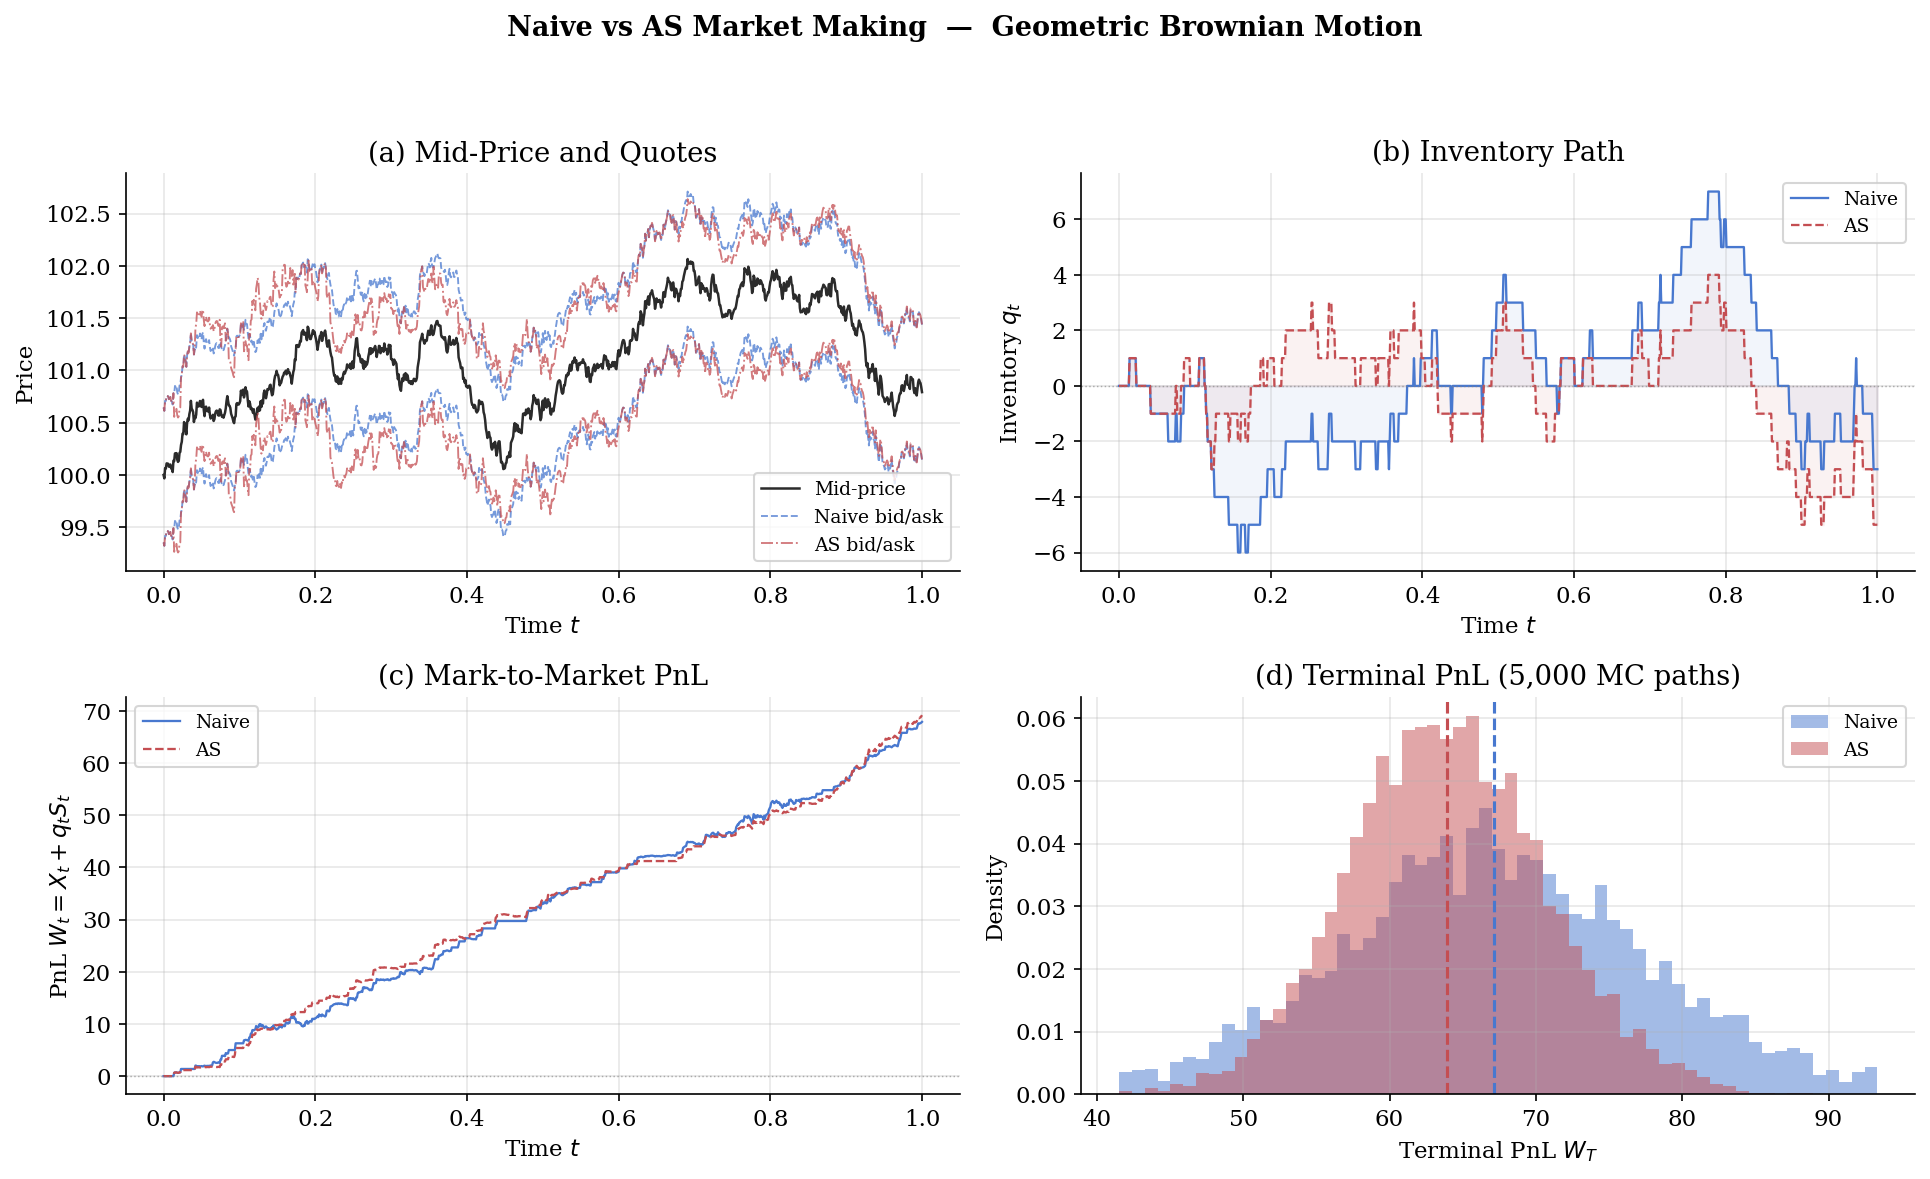
\includegraphics[width=0.85\textwidth]{img/hft1-py2.png}
\caption{Single-asset GBM comparison: naive versus Avellaneda--Stoikov quoting.}
\label{hft1-fig:gbm_results}
\end{figure}

Figure~\ref{hft1-fig:gbm_results} reports the GBM case. Since $\sigma_{GBM}S_0$ is calibrated to match the ABM dollar volatility, the aggregate Monte Carlo diagnostics are close to the ABM case. The difference is conceptual rather than cosmetic. Under GBM, the volatility parameter describes return risk, while the risk of holding one physical unit of inventory depends on the current price level. For this reason, the simulation uses the local monetary variance approximation $(\sigma_{GBM}S_t)^2$ inside the reservation price. When $S_t$ increases, one unit of inventory becomes riskier in dollar terms, and the AS quote skew reacts more strongly. This is why the GBM version is useful even if the numerical table is similar to ABM: it shows that inventory control should be expressed in monetary-risk units, not directly in return-volatility units.

\subsection{Covariance-Aware Multi-Asset Diagnostics}

The multivariate experiment uses three correlated arithmetic Brownian assets. Asset C is deliberately specified as inversely correlated with the first two assets, so that the covariance pressure $\Sigma q_t$ can differ sharply from the raw inventory vector $q_t$. This makes the key multi-asset mechanism visible: a position that looks large in physical units may be less dangerous if it hedges the rest of the book, while a small position may still be risky if it loads on the same covariance direction as the current portfolio.

\begin{figure}[H]
\centering
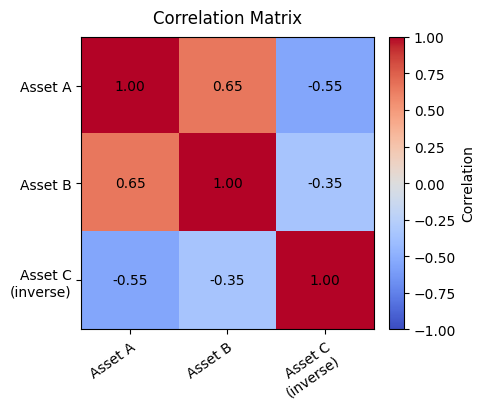
\includegraphics[width=0.58\textwidth]{img/hft1-Corr.png}
\caption{Correlation matrix used in the three-asset diagnostic. The matrix has unit diagonal entries, with $\rho_{AB}=0.65$, $\rho_{AC}=-0.55$, and $\rho_{BC}=-0.35$. Positive values indicate co-movement between assets, while negative values capture the inverse exposure of Asset C.}
\label{hft1-fig:correlation-matrix-three-asset}
\end{figure}

The corresponding covariance matrix $\Sigma$ combines these correlation coefficients with the individual asset volatilities. It is the matrix used by the covariance-aware policy to transform the raw inventory vector $q_t$ into the risk-pressure vector $\Sigma q_t$.

\begin{table}[H]
\centering
\small
\caption{Covariance matrix $\Sigma$ used in the three-asset diagnostic.}
\begin{tabular}{@{}lrrr@{}}
\toprule
 & Asset A & Asset B & Asset C (inverse) \\
\midrule
Asset A           &  2.2500 &  1.0725 & -0.7425 \\
Asset B           &  1.0725 &  1.2100 & -0.3465 \\
Asset C (inverse) & -0.7425 & -0.3465 &  0.8100 \\
\bottomrule
\end{tabular}
\end{table}

For $N=3{,}000$ Monte Carlo paths, the covariance-aware inventory policy again sacrifices a small amount of average PnL but materially improves the risk profile of the terminal book.

\begin{table}[H]
\centering
\small
\caption{Multivariate Monte Carlo diagnostics with $3{,}000$ simulated paths.}
\begin{tabularx}{\textwidth}{@{}Xrrr@{}}
\toprule
Metric & Naive & Inventory-based & Difference \\
\midrule
Mean terminal PnL                         & 158.709 & 154.556 & -4.153 \\
Std terminal PnL                          &  16.439 &  10.547 & -5.892 \\
Sharpe-like ratio                         &   9.654 &  14.654 &  5.000 \\
Mean $|$terminal inv$|$                   &  21.949 &  11.203 & -10.745 \\
Mean Std$(q_t)$                           &   6.593 &   3.397 & -3.195 \\
Mean turnover                             & 266.641 & 257.767 & -8.874 \\
Mean terminal risk $\|q_T\|_\Sigma$       &  17.051 &   7.419 & -9.632 \\
Median terminal risk $\|q_T\|_\Sigma$     &  15.313 &   6.996 & -8.318 \\
Mean average path risk                    &  11.397 &   3.925 & -7.472 \\
Mean max path risk                        &  22.638 &  10.065 & -12.573 \\
\bottomrule
\end{tabularx}
\end{table}

The multivariate results are stronger than the single-asset results because the naive policy is not merely ignoring inventory size; it is ignoring the entire covariance structure. The mean terminal risk norm $\|q_T\|_\Sigma=\sqrt{q_T^\top\Sigma q_T}$ falls from $17.051$ to $7.419$, while the mean maximum path risk falls from $22.638$ to $10.065$. The average gross terminal inventory also falls by more than ten units. These diagnostics show that covariance-aware control does not simply reduce each position mechanically; it reduces the risk of the portfolio after correlations are taken into account.

\begin{figure}[H]
\centering
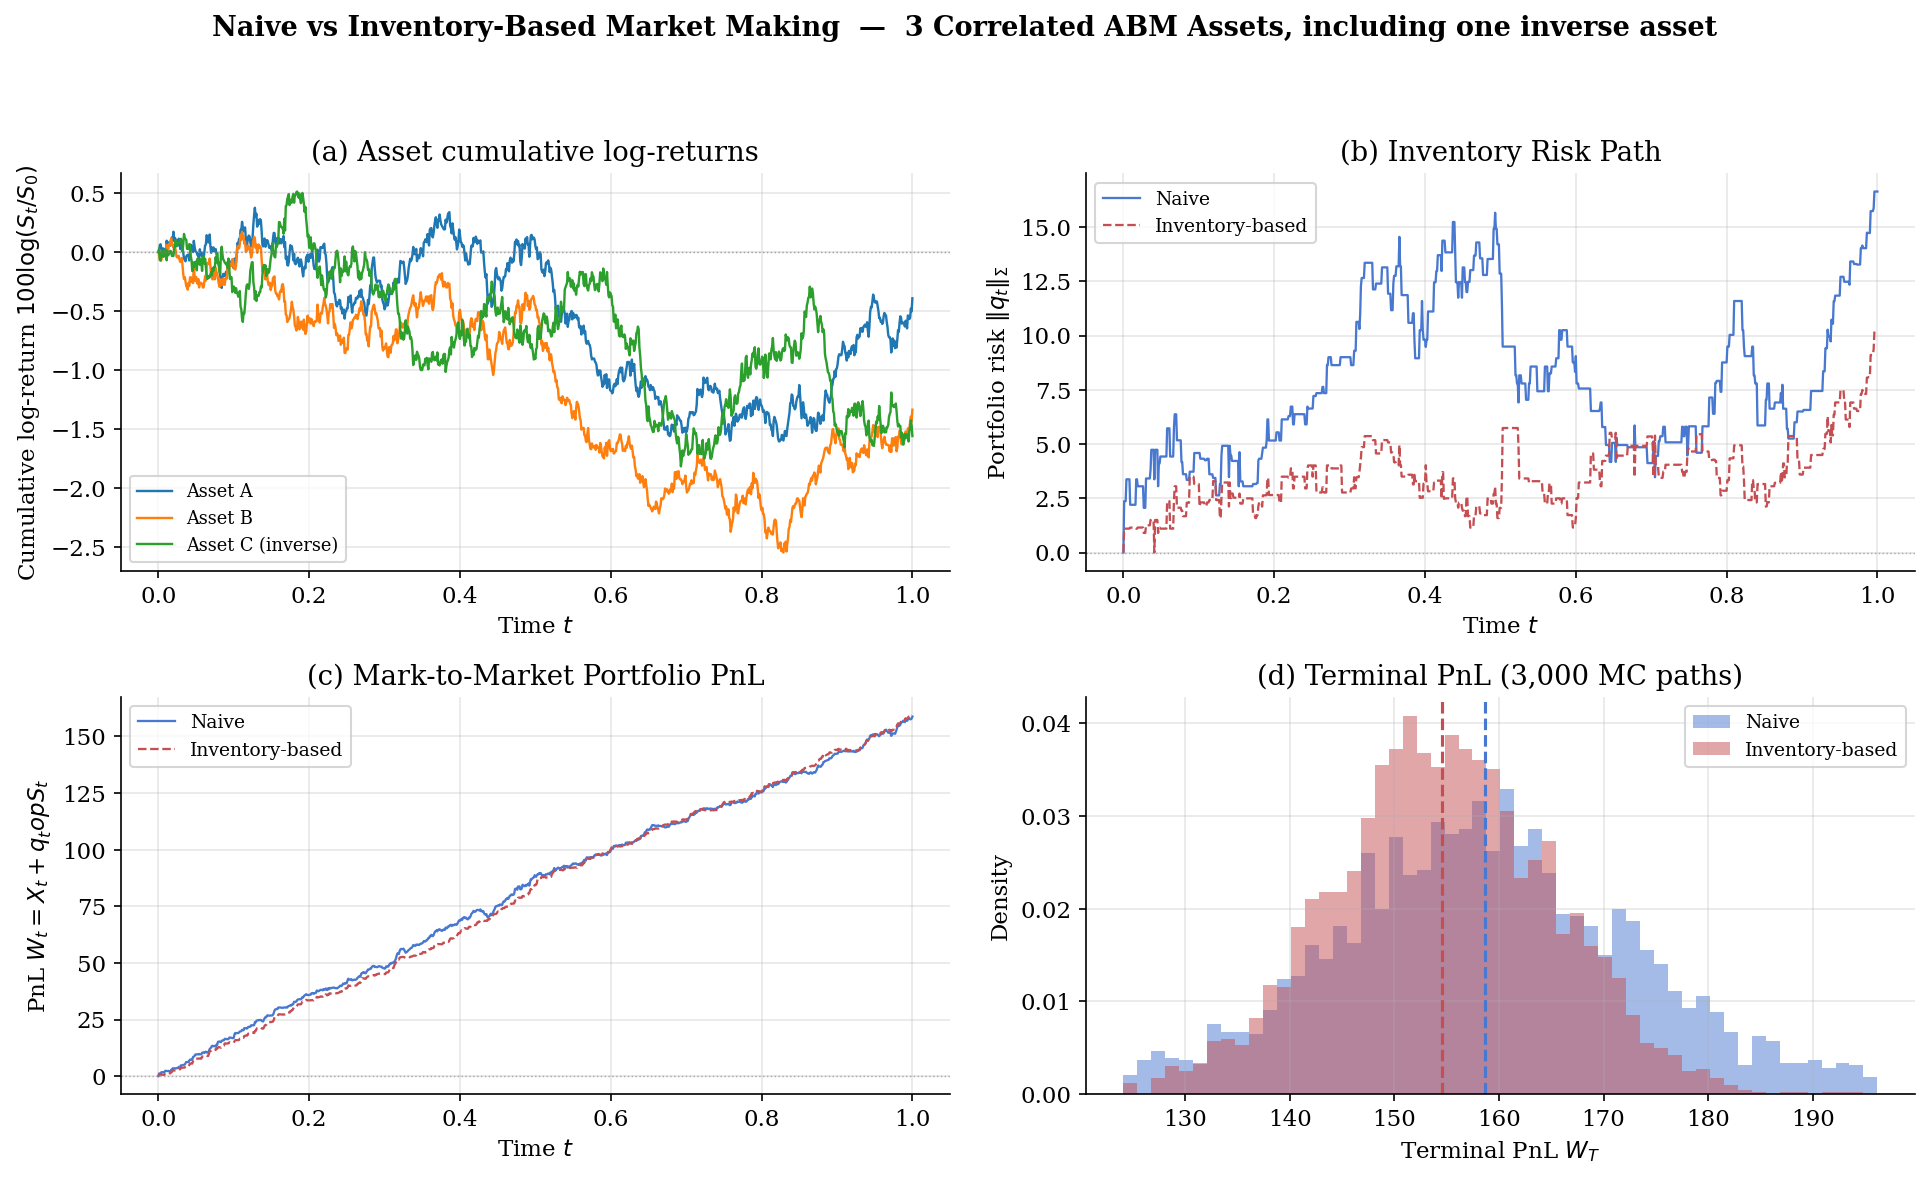
\includegraphics[width=0.96\textwidth]{img/hft1-py3.png}
\caption{Three-asset covariance-aware market-making diagnostic.}
\label{hft1-fig:multi_results}
\end{figure}

Figure~\ref{hft1-fig:multi_results} summarizes the three-asset diagnostic. Panel (a) reports cumulative log-returns, which makes the three price paths comparable even though the assets start from different price levels. The third asset is intentionally inversely correlated with the first two, so the relevant inventory signal is no longer the raw vector $q_t$ alone but the covariance-adjusted pressure $\Sigma q_t$. Panel (b) shows the portfolio risk norm $\|q_t\|_\Sigma$, which is the natural multivariate analogue of single-asset inventory risk. The naive strategy accumulates a much larger covariance-adjusted exposure because it treats each asset independently, while the inventory-based strategy keeps the risk path lower by reacting to the whole book. Panel (c) shows that both policies generate positive spread-capture PnL on the reference path, but the inventory-aware policy does so with a substantially lower portfolio-risk footprint. Panel (d) confirms the Monte Carlo result: the inventory-based terminal PnL distribution is more concentrated, while the naive policy leaves wider tails because it accepts larger covariance-adjusted inventory exposure. This is the key difference from the scalar case: the multi-asset dealer must control the risk of the book, not only the size of each single position.

Overall, the numerical evidence is consistent across all three experiments. The naive policy can look attractive if one only checks average PnL in a frictionless benchmark, but this comes from carrying more inventory risk. The Avellaneda--Stoikov policy is better understood as a risk-adjusted market-making rule: it reduces terminal inventory, lowers PnL volatility, and becomes especially valuable once the dealer manages a correlated book rather than a single isolated asset.

These covariance-aware diffusion results establish the inventory-risk mechanism before volatility memory and terminal liquidation are introduced in the next experiment.

The common finding in ABM, local-variance GBM and the correlated diffusion is reduced exposure and dispersion, with a lower mean PnL in the displayed samples. This does not establish a benefit from memory: none of these environments contains a rough volatility state. We therefore turn to a different experiment with a finite memory approximation and priced terminal liquidation.
\section{Finite-lift configurations with historical scalar controls}
The following 2000-session results use the historical clipped scalar solver and full finite-lift forward paths. They are retained as evidence for that implementation, not as a converged optimal-policy benchmark. Their $H$ labels refer to the weight prescription explained in Chapter~\ref{ch:control}.
\subsection{Diagnostics, figures, and representative close-out paths}

The numerical pipeline produces the diagnostics and the two figures included below. Figure~\ref{hft2-fig:hjb_surfaces} reports the initial HJB surfaces for all three Hurst regimes. These panels are easy to misread on a first pass, so it is useful to separate the interpretation carefully.

\begin{algorithm}[H]
\caption{Reading the HJB surface figure}
\DontPrintSemicolon
\For{each \(H\in\{0.2,0.5,0.8\}\)}{
  calibrate the lifted rough environment and compress it to the HJB state \(y\)\;
  solve the reduced HJB backward on the \((q,y)\) grid with liquidation terminal condition\;
  export \(\Theta(0,q,y)\), \(\delta^{b,*}(0,q,y)\), and \(\delta^{a,*}(0,q,y)\)\;
}
read rows by regime and columns by continuation value, bid offset, and ask offset\;
\end{algorithm}

\begin{figure}[H]
\centering
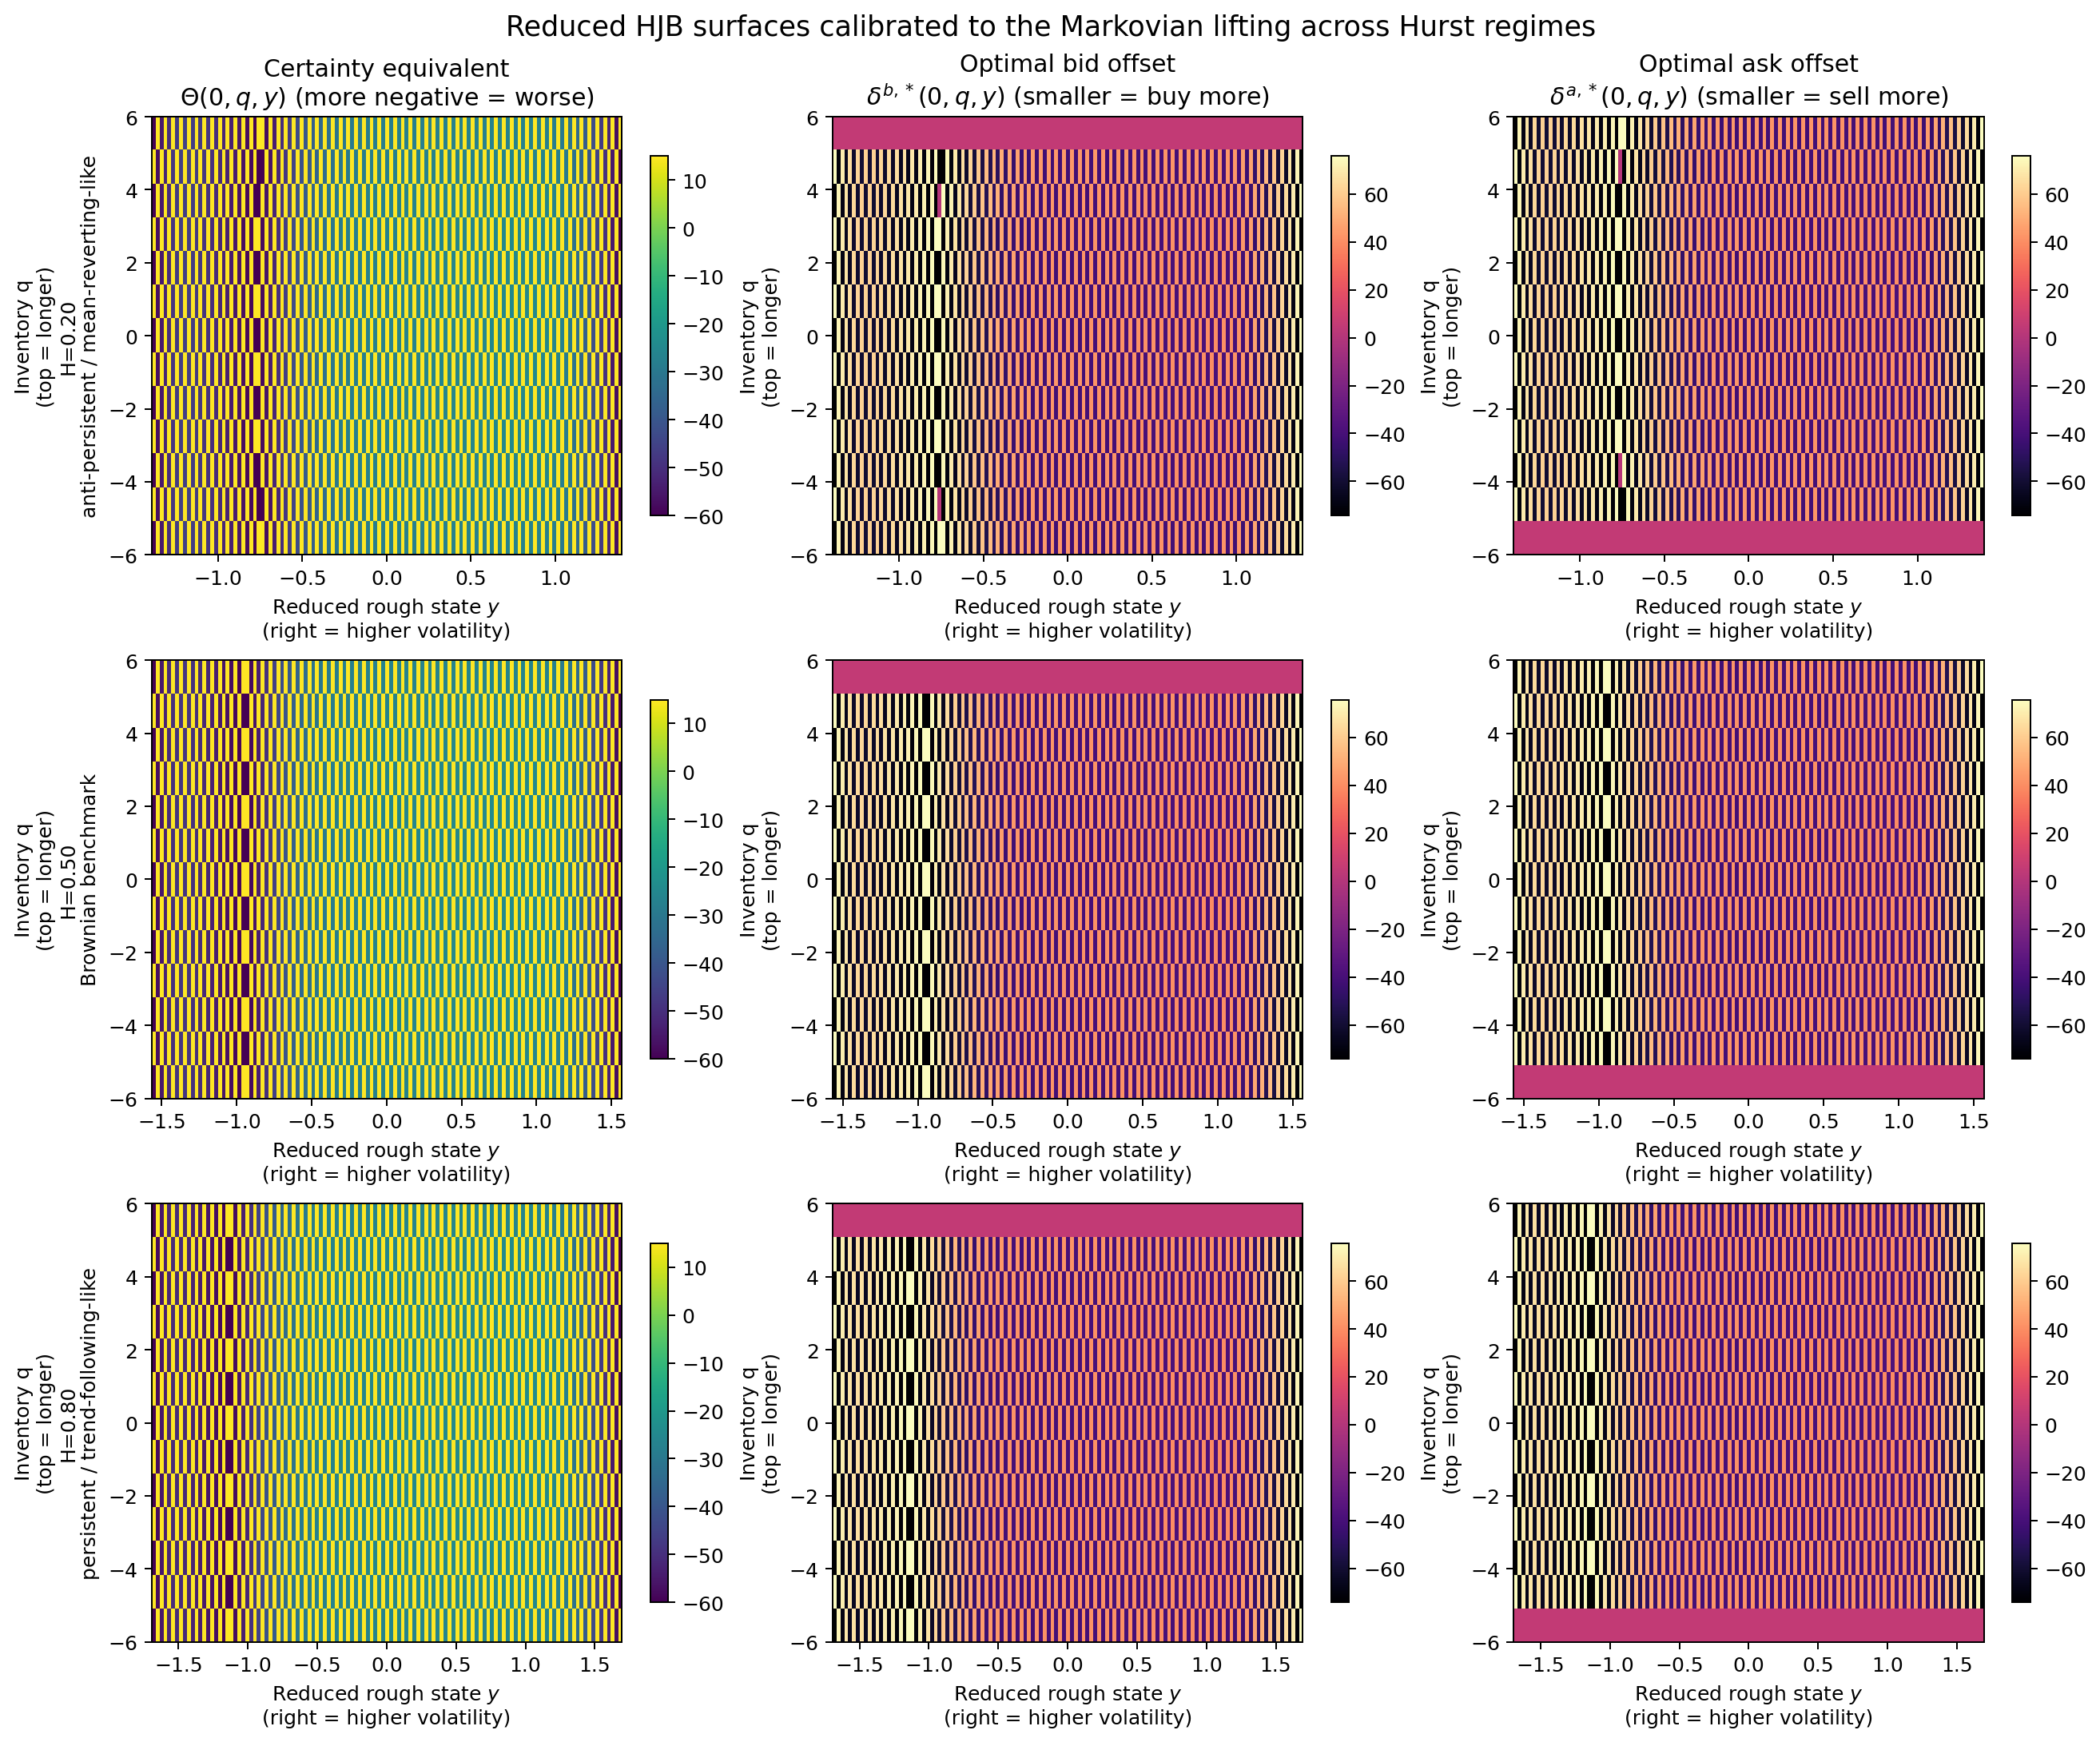
\includegraphics[width=\textwidth]{img/hft2-hjb_surfaces.png}
\caption{Reduced HJB surfaces across the three Hurst regimes. Each row corresponds to one lifted environment: \(H=0.2\) anti-persistent, \(H=0.5\) Brownian, and \(H=0.8\) persistent. The columns show the certainty-equivalent correction, the optimal bid offset, and the optimal ask offset at the initial time.}
\label{hft2-fig:hjb_surfaces}
\end{figure}

To read Figure~\ref{hft2-fig:hjb_surfaces}, fix one row first, so that \(H\) is held constant, and then move inside that row:
\begin{enumerate}[label=\arabic*.]
    \item The horizontal axis is the rough state \(y\). Moving to the right means a more stressed rough-volatility state and therefore a larger local variance forecast.
    \item The vertical axis is the inventory \(q\). Moving upward means the dealer is longer inventory; moving downward means the dealer is shorter inventory.
    \item In the first column, \(\Theta(0,q,y)\) is the continuation-value correction. More negative values mean that carrying that state forward is less attractive because future inventory risk and liquidation risk are more expensive.
    \item In the second column, \(\delta^{b,*}(0,q,y)\) is the optimal bid offset. A \emph{smaller} bid offset means the bid is closer to the mid-price, so the dealer buys more aggressively. A \emph{larger} bid offset means the dealer backs the bid away and becomes less willing to buy.
    \item In the third column, \(\delta^{a,*}(0,q,y)\) is the optimal ask offset. A \emph{smaller} ask offset means the ask is closer to the mid-price, so the dealer sells more aggressively. A \emph{larger} ask offset means the dealer is less willing to sell.
\end{enumerate}

The Avellaneda--Stoikov asymmetry is therefore read vertically. If one moves upward to positive inventory, the dealer should buy less aggressively and sell more aggressively: the bid offset widens, the ask offset tightens, and the certainty-equivalent surface deteriorates. If one moves downward to negative inventory, the pattern reverses. The effect of the rough state is read horizontally: moving toward larger \(y\) raises the volatility forecast, so both quotes tend to become more conservative overall, while the exact curvature changes across the three Hurst regimes.

The volatility diagnostics confirm that the environment remains genuinely stochastic in all three cases. The mean integrated variance changes only slightly, but the dispersion increases with \(H\), which is consistent with the fact that persistent regimes keep variance excursions alive for longer. This is why it is useful to report not only PnL and inventory, but also volatility statistics themselves.

\begin{table}[H]
\centering
\caption{Volatility diagnostics of the simulated environment across \(2{,}000\) trading days.}
\label{hft2-tab:hjb_vol_diagnostics}
\begin{tabular}{@{}lrrrr@{}}
\toprule
\(H\) & Mean realized vol & Std realized vol & Mean integrated var & Std integrated var \\
\midrule
0.20 & 1.096 & 0.081 & 1.209 & 0.155 \\
0.50 & 1.095 & 0.090 & 1.209 & 0.180 \\
0.80 & 1.095 & 0.098 & 1.208 & 0.199 \\
\bottomrule
\end{tabular}
\end{table}

Figure~\ref{hft2-fig:hjb_simulation} then collects one representative day for each regime. The left column shows the lifted rough state together with the induced local variance, the center column shows the inventory path from the open to the forced flat close, and the right column compares the end-of-day liquidated PnL distributions of the naive and HJB strategies. The reported pattern is shared by these three configurations: the HJB policy consistently keeps much less inventory into the close, which translates into a much smaller liquidation bill.

\begin{algorithm}[H]
\caption{Reading the close-out simulation figure}
\DontPrintSemicolon
\For{each simulated trading day}{
  update the lifted rough state and map it into local variance\;
  simulate the mid-price and order arrivals under common random numbers\;
  compare naive symmetric quoting with the HJB inventory-aware policy\;
  force terminal liquidation, record close-out cost, PnL, and inventory diagnostics\;
}
select one representative path per regime and plot it beside the Monte Carlo PnL histograms\;
\end{algorithm}

The representative path is now selected separately inside each regime, which is the natural choice once the forward simulation uses the full lifted state and the three Hurst cases no longer share the same effective trajectory. Table~\ref{hft2-tab:hjb_representative_path} makes the close-out mechanics explicit. In every regime the HJB policy still arrives at the close with materially smaller inventory and therefore a much smaller liquidation bill than the naive benchmark.

\begin{table}[H]
\centering
\caption{Representative regime-specific paths from Figure~\ref{hft2-fig:hjb_simulation}.}
\label{hft2-tab:hjb_representative_path}
\begin{tabular}{@{}lrrrrrrr@{}}
\toprule
\(H\) & Seed & \(q_{T^-}^{\mathrm{naive}}\) & \(q_{T^-}^{\mathrm{HJB}}\) & \(L^{\mathrm{naive}}\) & \(L^{\mathrm{HJB}}\) & PnL\(_{\mathrm{naive}}\) & PnL\(_{\mathrm{HJB}}\) \\
\midrule
0.20 & 218 & 4.000 & -1.000 & 6.290 & 1.032 & -1.349 & 2.533 \\
0.50 & 250 & 4.000 & 1.000 & 6.719 & 1.140 & 5.544 & 8.833 \\
0.80 & 235 & 6.000 & 2.000 & 11.816 & 2.499 & 1.087 & 2.886 \\
\bottomrule
\end{tabular}
\end{table}

\begin{figure}[H]
\centering
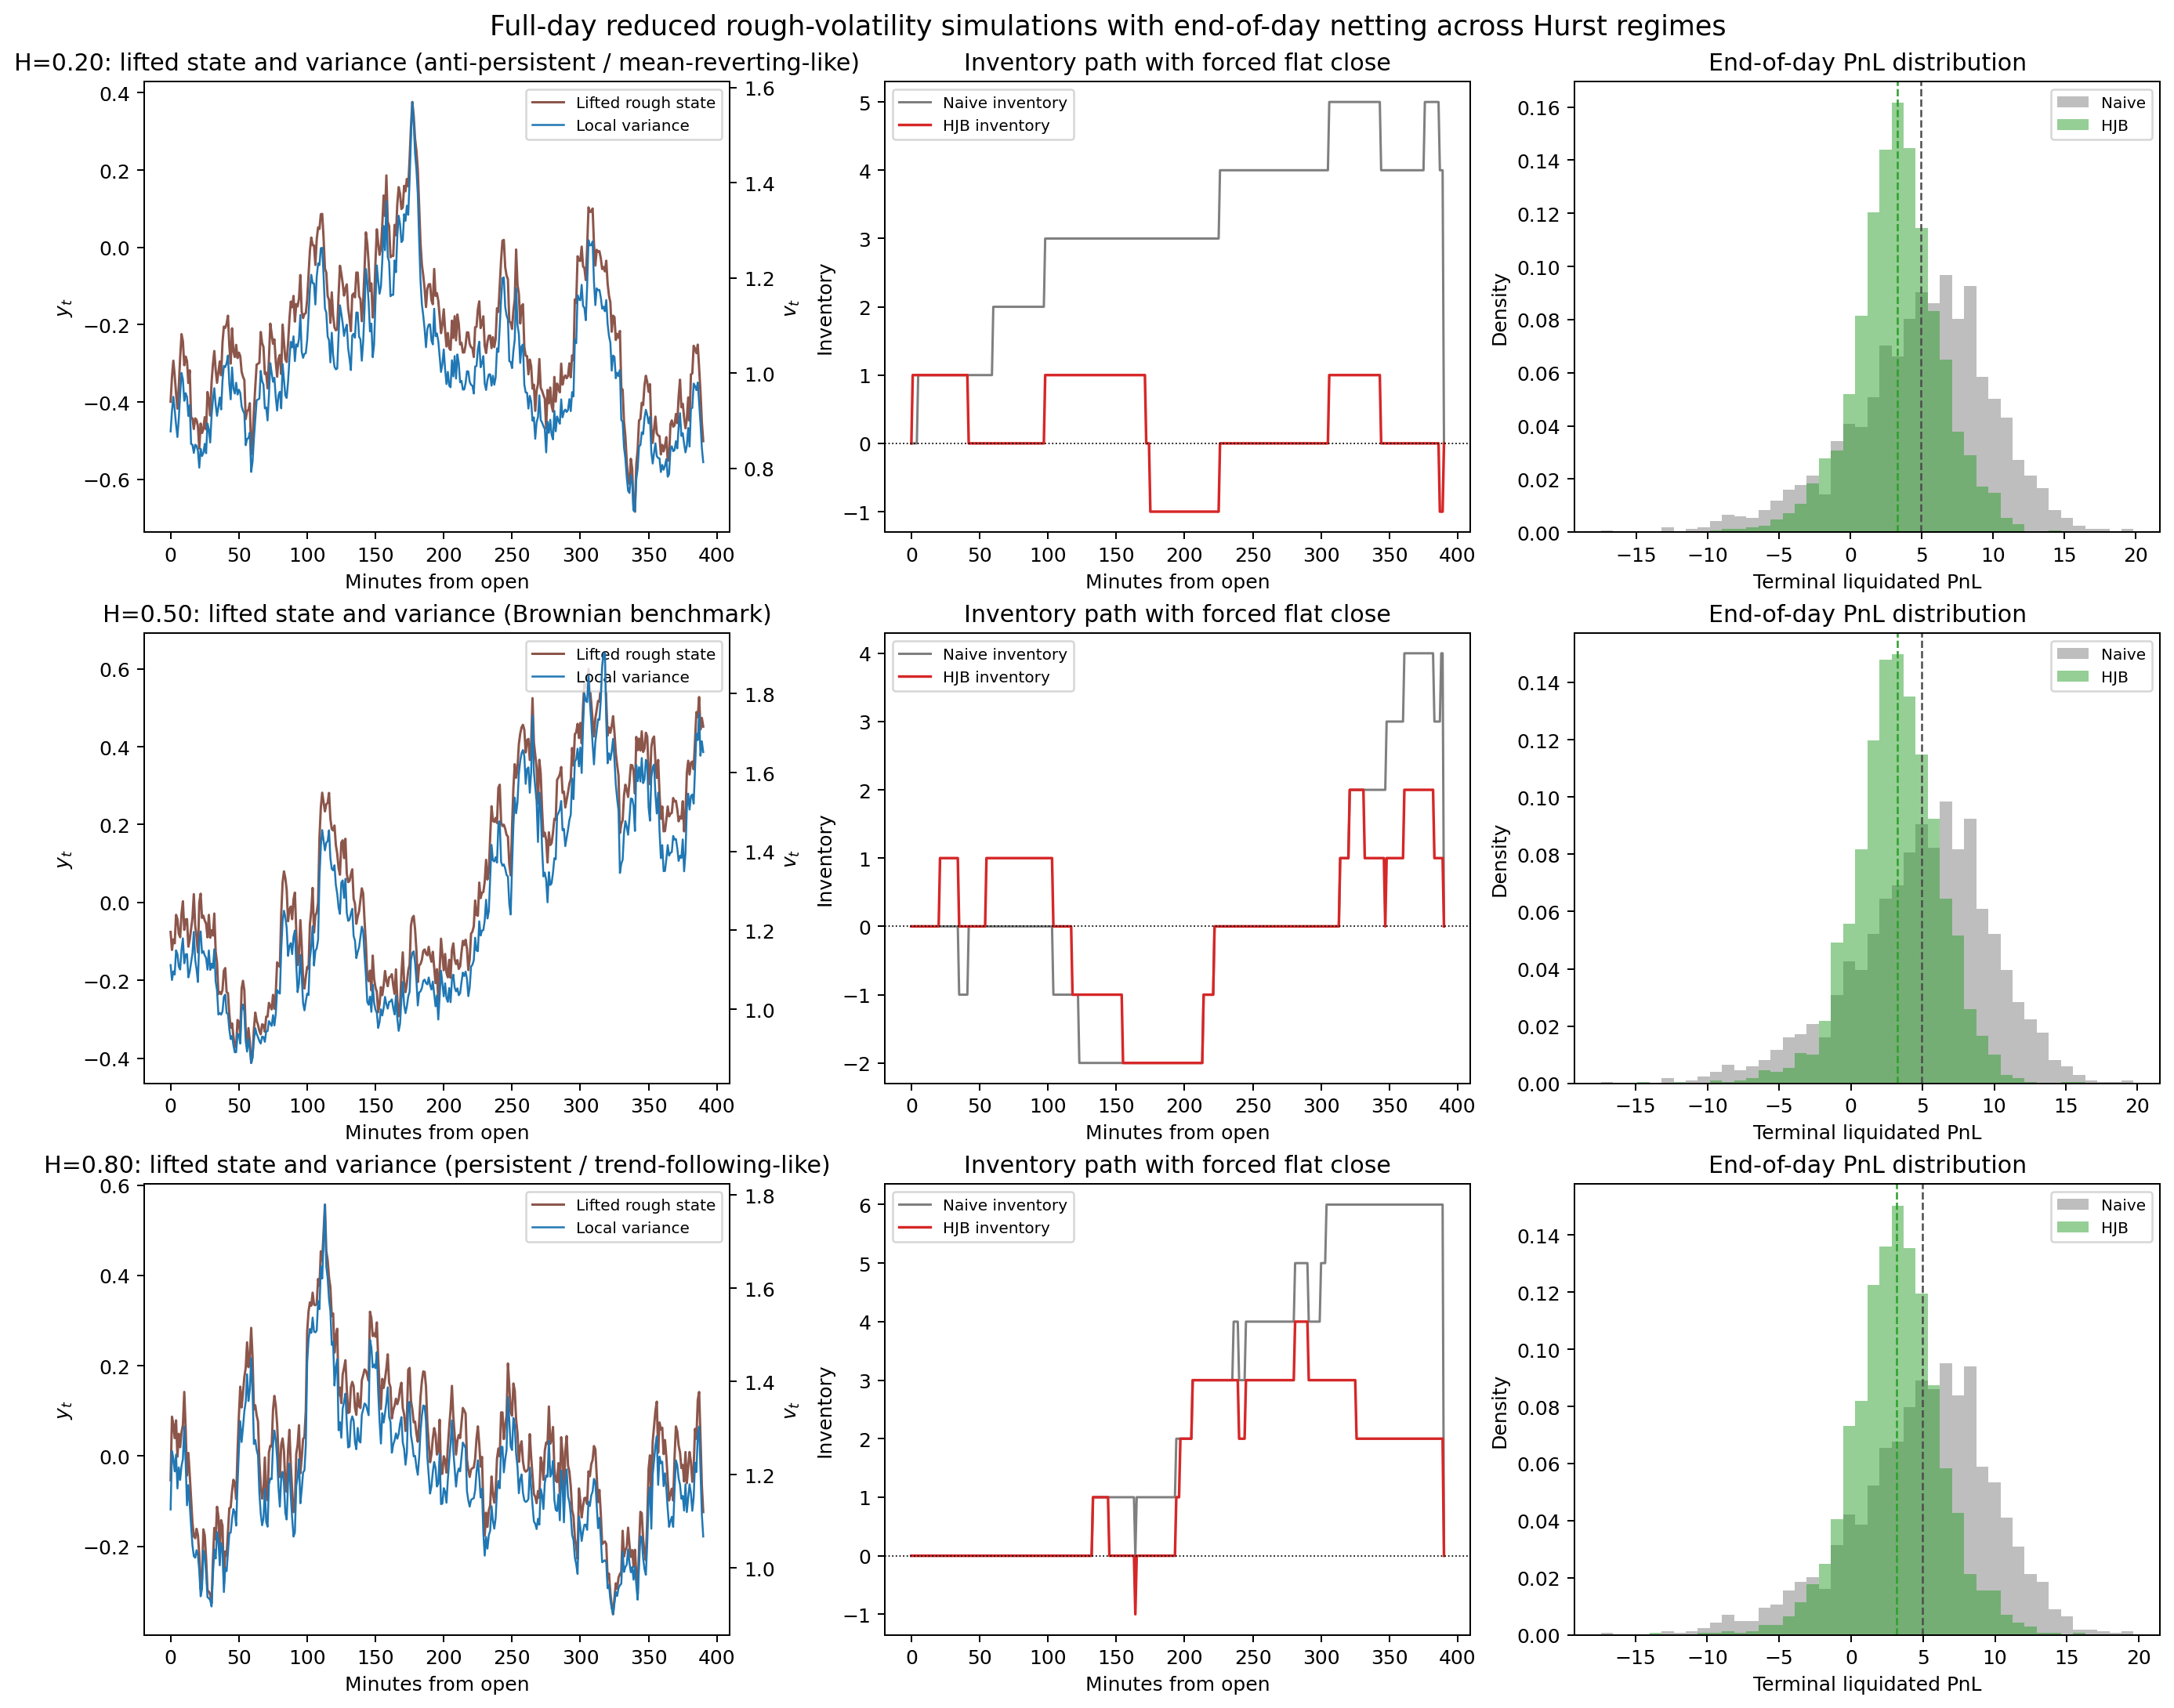
\includegraphics[width=\textwidth]{img/hft2-hjb_simulation.png}
\caption{Representative full-day simulations and Monte Carlo histograms across the three Hurst regimes. Rows correspond to \(H=0.2\), \(H=0.5\), and \(H=0.8\); columns show the lifted rough state and local variance, the inventory path with forced flat close, and the end-of-day liquidated PnL distribution.}
\label{hft2-fig:hjb_simulation}
\end{figure}

\subsection{Monte Carlo evidence and interpretation}

The full Monte Carlo comparison is reported in Tables~\ref{hft2-tab:hjb_mc_risk} and \ref{hft2-tab:hjb_mc_inventory}. Several points are worth separating carefully.

First, the naive benchmark keeps the larger \emph{mean} PnL in every regime. This is not a contradiction of Avellaneda--Stoikov. A symmetric spread-capture strategy can earn more average PnL precisely because it is willing to warehouse inventory and postpone the risk accounting until the close. The relevant question is therefore not ``which policy has the largest raw mean PnL?'', but rather ``what happens after one charges the close-out risk consistently?''

Second, on the dimensions that measure end-of-day inventory risk directly, the displayed historical HJB sample is better. In all three regimes the average pre-close inventory falls from about \(2.50\) to roughly \(0.55\), and the average liquidation cost falls from about \(3.99\) to roughly \(0.67\). The left tail also improves materially: the 5\% expected shortfall is less negative in every case.

\begin{table}[H]
\centering
\caption{Risk-adjusted Monte Carlo comparison with forced net-zero close (\(2{,}000\) sessions).}
\label{hft2-tab:hjb_mc_risk}
\begin{tabular}{@{}lrrrrrr@{}}
\toprule
\(H\) & Sharpe\(_N\) & Sharpe\(_H\) & CE\(_N\) & CE\(_H\) & ES\(_N\) & ES\(_H\) \\
\midrule
0.20 & 1.017 & 1.110 & 2.052 & 2.352 & -6.870 & -3.607 \\
0.50 & 1.017 & 1.082 & 2.056 & 2.208 & -6.865 & -3.734 \\
0.80 & 1.018 & 1.034 & 2.059 & 2.156 & -6.862 & -3.681 \\
\bottomrule
\end{tabular}
\end{table}

\begin{table}[H]
\centering
\caption{Inventory and liquidation metrics across the three Hurst regimes.}
\label{hft2-tab:hjb_mc_inventory}
\begin{tabular}{@{}lrrrrrr@{}}
\toprule
\(H\) & Mean PnL\(_N\) & Mean PnL\(_H\) & \(\E|q_{T^-}|_N\) & \(\E|q_{T^-}|_H\) & \(\E L_N\) & \(\E L_H\) \\
\midrule
0.20 & 4.955 & 3.309 & 2.504 & 0.547 & 3.990 & 0.654 \\
0.50 & 4.957 & 3.244 & 2.504 & 0.572 & 3.989 & 0.693 \\
0.80 & 4.958 & 3.173 & 2.504 & 0.549 & 3.988 & 0.667 \\
\bottomrule
\end{tabular}
\end{table}

The interpretation of the three regimes is now cleaner than before. For \(H=0.2\), the anti-persistent rough driver is the most favorable case for the HJB: the strategy gives up some mean PnL, but it improves Sharpe, certainty equivalent, and tail risk while dramatically shrinking the liquidation bill. For \(H=0.5\), the Brownian benchmark still leaves more raw spread-capture income to the naive policy, yet the historical sample favors the HJB on Sharpe, certainty equivalent, inventory discipline, and close-out cost. For \(H=0.8\), the persistent regime remains the hardest case in the sense that the risk-adjusted gain becomes smaller, but even there the reported HJB sample improves Sharpe, improves certainty equivalent, improves expected shortfall, and cuts liquidation cost by a large margin.

This is precisely where the earlier conceptual discussion matters. Avellaneda--Stoikov formulates a Markovian utility-maximization problem, not universal dominance in raw mean PnL after one changes the environment and adds forced end-of-day liquidation. In the present implementation, the naive benchmark still wins on average PnL because it warehouses inventory more aggressively. The historical HJB sample, however, has better reported metrics on the dimensions that actually price inventory risk correctly at the close.

The practical conclusion is therefore sharper. If one optimizes only raw mean PnL, the naive benchmark can still look attractive because it monetizes spread capture by tolerating much larger end-of-day inventory. Once one cares about close-out discipline, liquidation cost, certainty equivalent, and left-tail protection, the historical tables favor inventory-aware quotes on the reported risk-sensitive metrics in all three configurations.

These historical comparisons motivate the next check: whether the same inventory-control mechanism remains useful when the scalar solve uses positive bounded-control evolution instead of value clipping.
\section{A positive baseline in its scalar and lifted environments}
The historical clipped results above and the following positive-baseline replay answer different numerical questions. The policy and simulation configuration change, so a larger PnL here cannot be read as the isolated causal effect of repairing the solver. Within E1 and E2, however, the policy/naive comparison uses common shocks and consistent liquidation accounting.

The surfaces become a trading strategy through a feedback loop. At each simulated time, interpolate the solved certainty equivalent in $(t,Y)$ at the current discrete inventory, compute neighboring-inventory gains and apply the bounded Hamiltonian. The resulting offsets give $p_b=S-\delta_b$ and $p_a=S+\delta_a$. A dealer buy changes $(X,q)$ to $(X-p_b,q+1)$; a sale changes it to $(X+p_a,q-1)$. The next decision uses this updated inventory. A quote is not a guaranteed execution, and a price crossing is not the execution rule in this arrival-intensity model.

The illustrative simulator uses 3900 intervals over $T=1$, initial price 100, zero cash and inventory, and stationary volatility states. E1 uses the scalar OU model in which P2 was solved. E2 uses six common-noise OU factors with rates from 3 to 180 and normalized weights proportional to $\lambda^{-0.7}$. The price shock is independent of volatility. OU updates are exact on the grid; price and volatility are frozen during each interval's arrival processing, then price is advanced by its diffusion step. This splitting still requires time-step validation.

Candidate orders follow a Poisson process of rate $2A=28$, with equally likely sides and acceptance probability $\exp(-k\delta)$. Multiple candidates in an interval are processed sequentially, updating inventory and quotes after each fill. Both strategies share candidate counts, side marks, uniforms and the market path. The naive comparator uses constant symmetric offset $\log(1+\gamma/k)/\gamma$ and the same inventory limits. At $T$, liquidated wealth is $X_T+q_TS_T-L(q_T,Y_T)$ and inventory is reset to zero. This cost is charged once; no other fees are included.

Figure~\ref{hft3-fig:market-e2} provides the missing price--quote--inventory application. It uses seed 42 and path zero, fixed independently of which strategy wins. Green quotes determine the green inventory path through executions. The displayed path need not have smaller P2 inventory at every time; performance is assessed over the collection of paths. Crosses in the wealth panel show the terminal deduction rather than disguising it as continuous trading profit.

\begin{figure}[p]
\centering
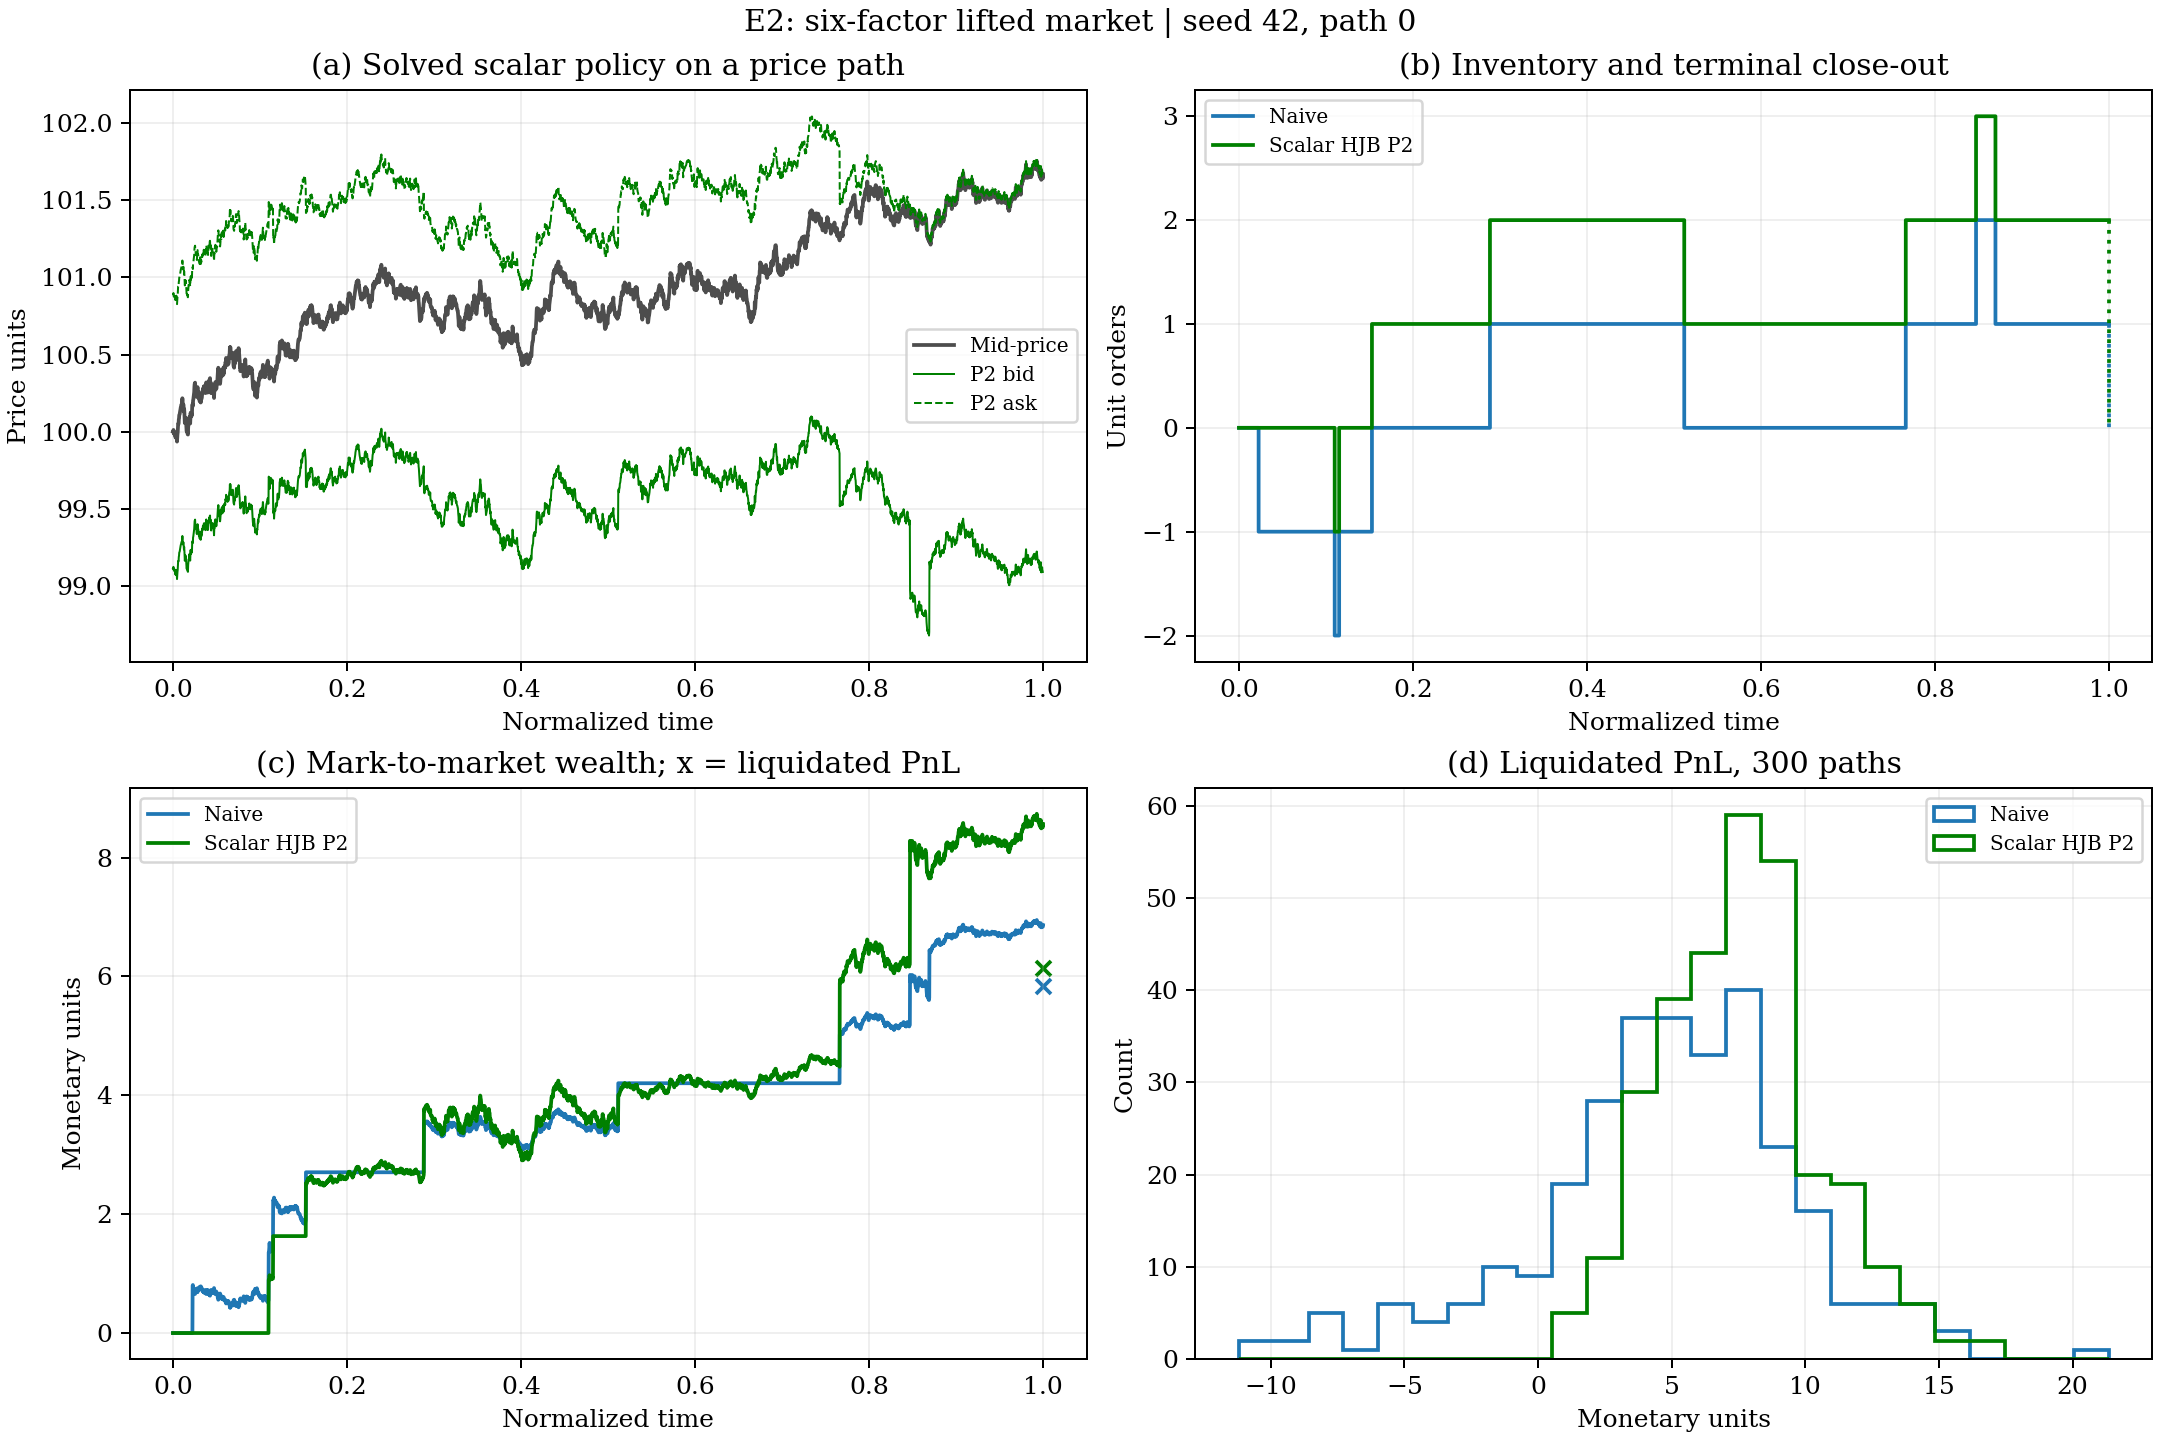
\includegraphics[width=\textwidth]{img/hft3-market_session_E2.png}
\caption{Baseline policy applied to the six-factor market E2. Top: price with P2 quotes and inventory for P2/naive. Bottom: marked wealth with liquidated terminal outcomes, and a common-bin histogram over 300 paired paths. Initial $S=100$, $X=q=0$, $T=1$, 3900 intervals, seed 42. This is P2 applied to a lifted environment, not a fitted HFT3 correction.}
\label{hft3-fig:market-e2}
\end{figure}

For E1, mean absolute inventory before liquidation is 2.433 for naive and 0.450 for P2; mean liquidated PnL is 5.445 and 7.724. For E2, these figures are 2.613 versus 0.427 and 4.792 versus 7.607. The mean paired PnL difference is 2.279 (standard error 0.215) in E1 and 2.816 (standard error 0.240) in E2. Comparisons are within each environment, not between the two sets of random paths. These synthetic baseline results do not demonstrate a correction benefit, global optimality or computational efficiency.

Checks enforce inventory limits, side disabling, exact-grid interpolation and the cash/inventory accounting identity, with maximum floating-point discrepancy $1.28\times10^{-13}$. No lookup leaves the exported state domain in these runs. The nearly singular OU innovation covariance is factored spectrally, removing only roundoff-negative eigenvalues: reconstruction error is $4.34\times10^{-19}$. The independent HJB residual, interpolation refinement and simulation-step convergence remain open. Consequently this experiment is an illustrative application, not the final validation gate for fitting P3.

\clearpage

\section{Adding stochastic covariance to separate policies}
The previous experiment tested the scalar policy against symmetric quotes. We now hold the positive baseline fixed and compare separate asset policies with the explicit covariance proxy from Chapter~\ref{ch:control}. This isolates a cross-inventory modification, not a transition from a Markovian to a non-Markovian model: the full twelve-factor environment remains finite-dimensional and Markovian.

Both strategies begin with $q=(3,0)$, prices $(100,100)$ and cash $-300$, so initial marked wealth is zero. This deliberately exposes the cross-asset response to a long A position. For each asset the inventory limit is six units and the arrival parameters remain $A=14$, $k=1.15$. One marked Poisson candidate stream of total rate 56 chooses asset and side uniformly; acceptance probability is $e^{-k\delta}$. Inventory and both assets' quotes are updated after every accepted candidate. Common candidates and exogenous shocks pair the two policies. Price and volatility remain frozen during each interval's arrivals, followed by diffusion updates. All assets are liquidated at $T$ and the sum of the two declared liquidation costs is charged once.

Figure~\ref{hft3-fig:multi-inventory} shows path zero under seed 73, fixed independently of the outcomes. Purple B inventory initially becomes short while A is long. Later, when positions and prices have evolved differently, the same policy can carry more risk than the separate policy. The selected path is illustrative; it is not required to exhibit the average ranking at every time.

\begin{figure}[p]
\centering
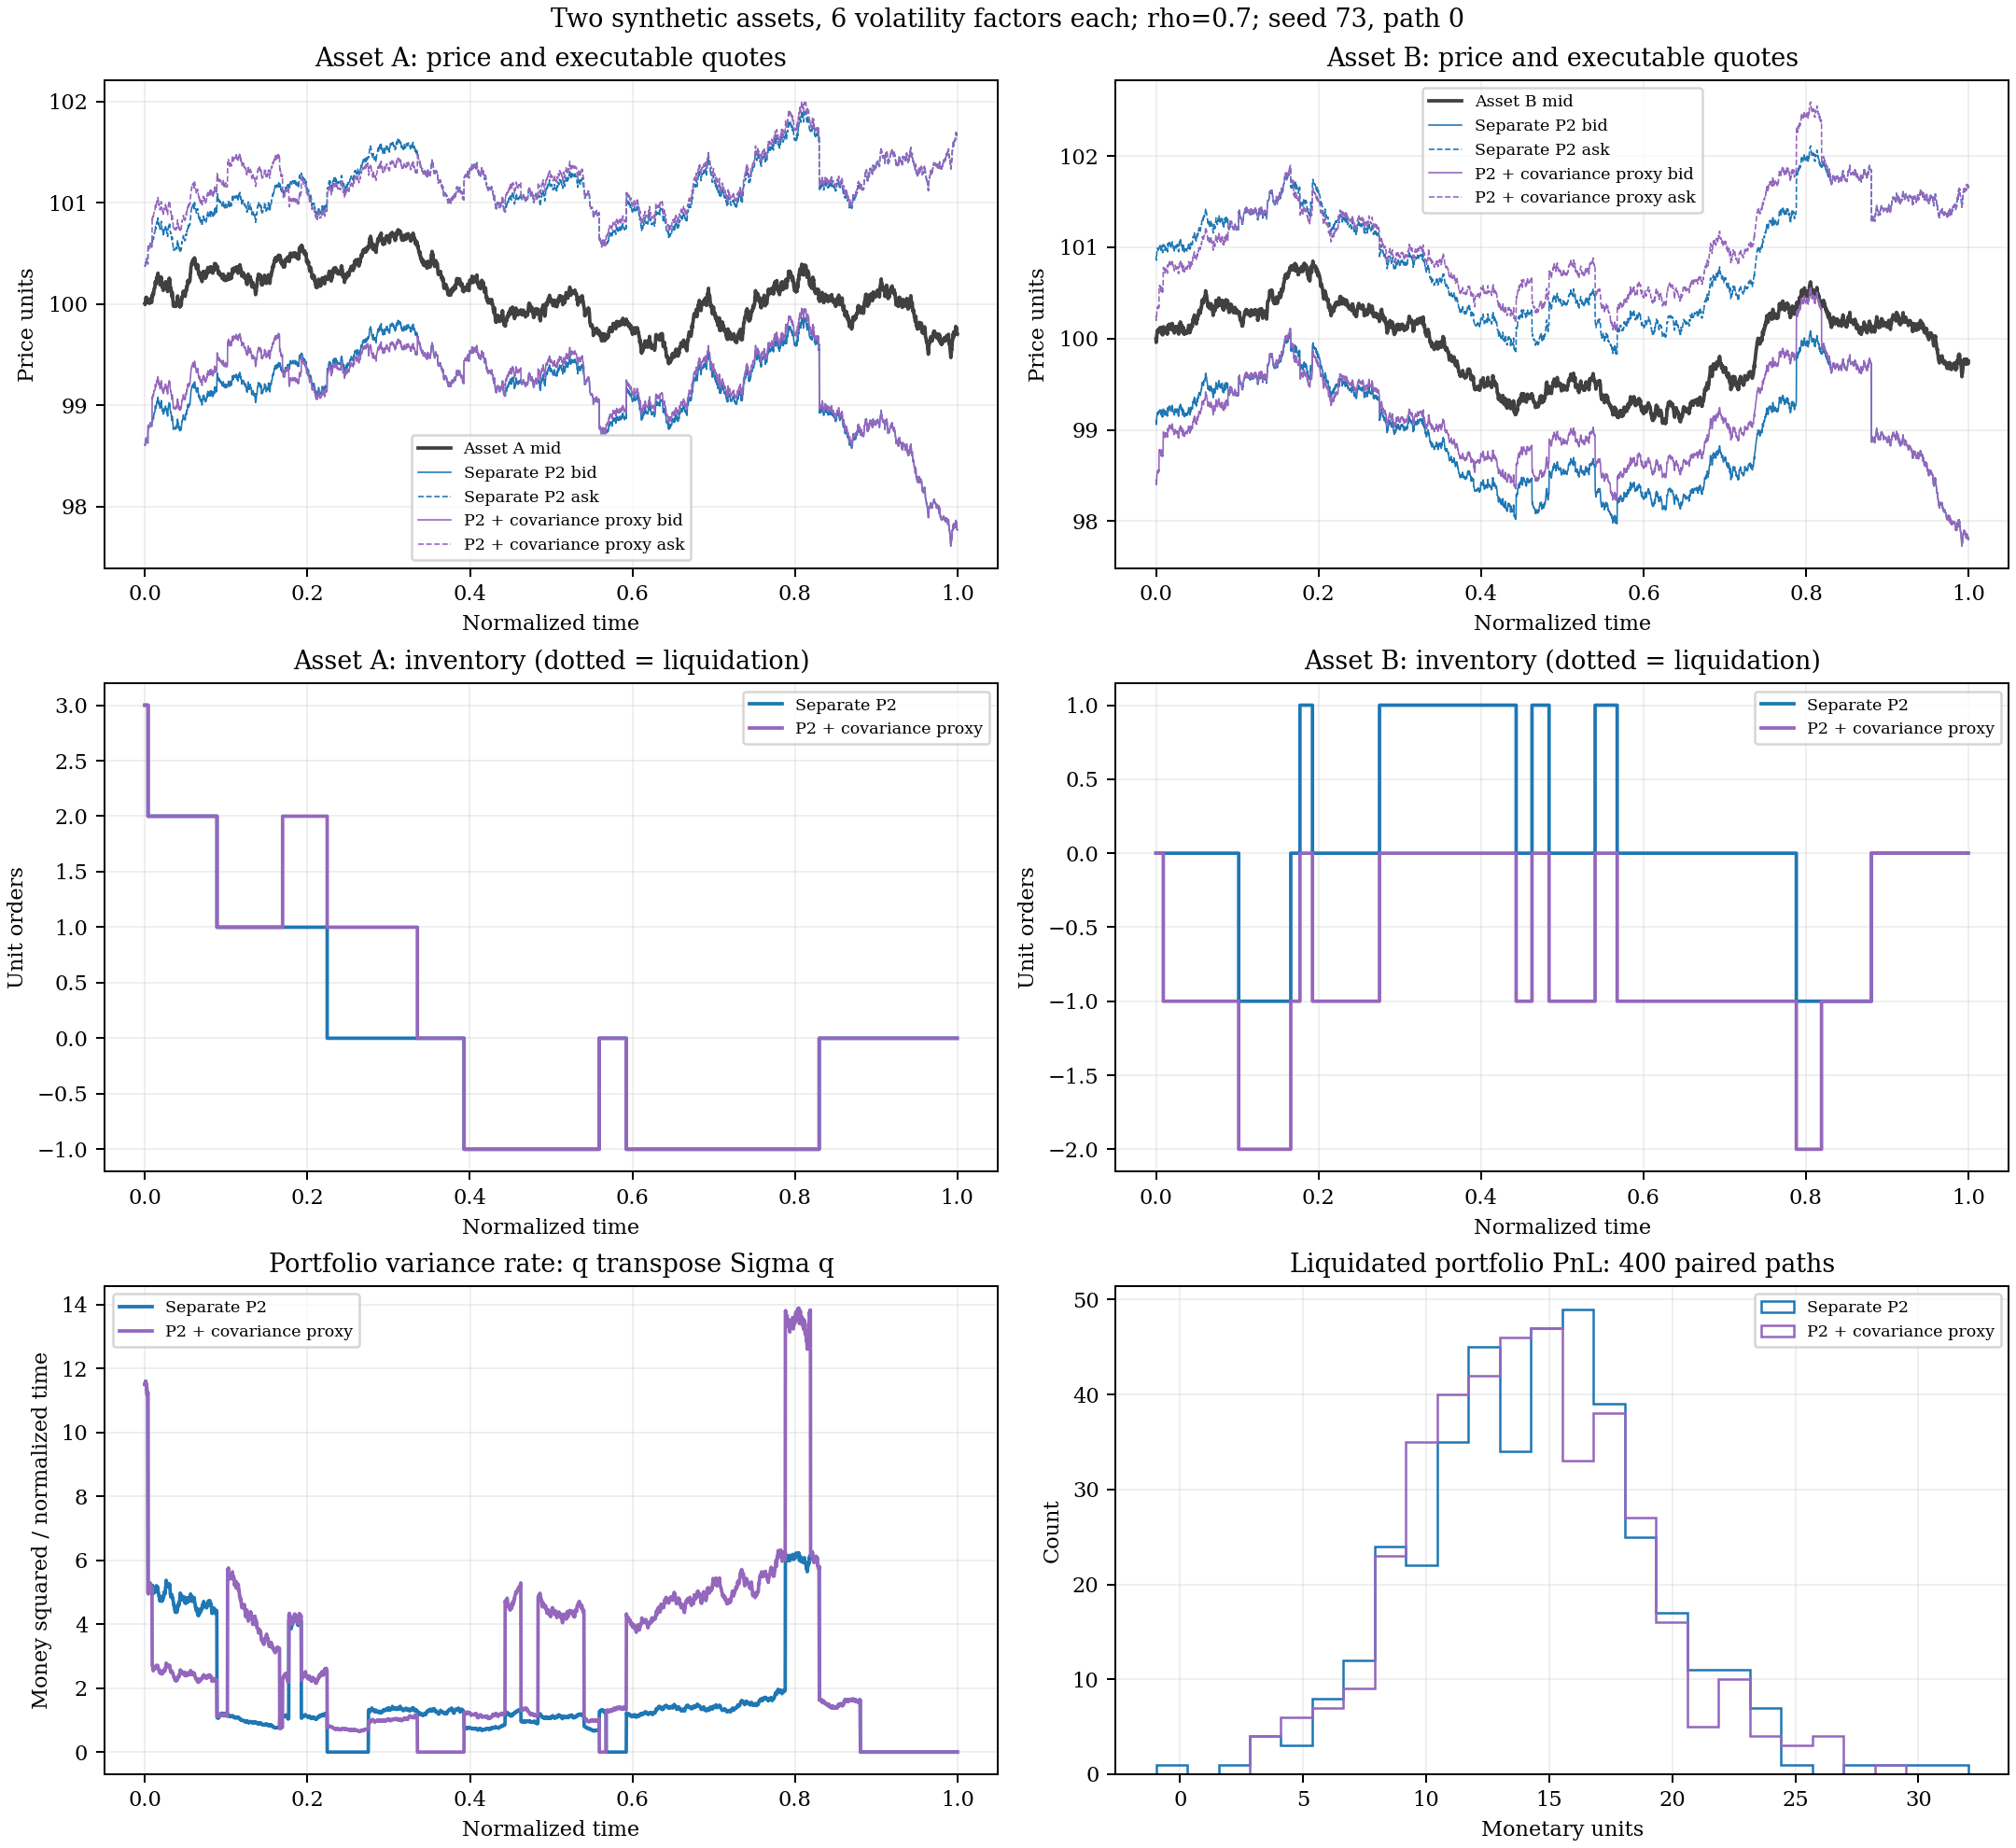
\includegraphics[width=\textwidth]{img/hft3-multiasset_inventory.png}
\caption{Two-asset application of separate P2 and P2 plus the covariance proxy. Top: both price paths and executable quotes. Middle: both inventories, with terminal liquidation dotted. Bottom: portfolio variance rate on the fixed illustrative path and liquidated PnL over 400 paired paths. Main run: 3900 intervals, price correlation 0.7, volatility-driver correlation 0.35, seed 73. The proxy is not the fitted residual-corrected policy P3.}
\label{hft3-fig:multi-inventory}
\end{figure}

For the main 400-path experiment, the results are
\begin{center}
\begin{tabular}{@{}lrr@{}}
\toprule
Metric & Separate P2 & Covariance proxy\\
\midrule
Mean $\int_0^Tq_t^\top\Sigma_tq_t\,dt$ & 5.8443 & 4.9608\\
Mean liquidated PnL & 14.4335 & 14.0905\\
Sample CARA certainty equivalent & 12.3054 & 12.2345\\
Mean $|q_A|$ before liquidation & 0.5275 & 0.5300\\
Mean $|q_B|$ before liquidation & 0.4825 & 0.5200\\
\bottomrule
\end{tabular}
\end{center}
The integrated-risk difference (proxy minus separate) is $-0.8835$, with paired standard error 0.1085: approximately 15.1\% lower mean integrated variance. This metric measures accumulated instantaneous inventory risk, not the sample variance of terminal PnL. The mean PnL difference is $-0.3430$, with paired standard error 0.0908. The sample certainty equivalent $-\log(\operatorname{mean}e^{-\gamma\mathrm{PnL}})/\gamma$ also decreases slightly; the conditional bootstrap interval for this nonlinear statistic is reported in the comparative-results chapter. The experiment therefore does not establish an improvement in the CARA objective. It shows a risk--revenue trade-off and motivates a better correction rather than validating this proxy as optimal.

A 1950-interval diagnostic with 400 paths has the same qualitative average trade-off: integrated variance 5.9781 versus 5.2543, PnL 13.9323 versus 13.6632. These two resolutions do not certify convergence. Reusing a seed at a different step count does not couple identical Brownian paths across resolutions; pairing is within each run. A separate zero-price-correlation regression produces identical inventories, cash and outcomes for both policies, even though the volatility drivers retain correlation 0.35. Thus this correction isolates price-covariance inventory coupling, not every source of dependence.
\section{A stochastic-covariance residual diagnostic}
For $\theta_{sep}=\theta_0(t,q_A,Y_A)+\theta_0(t,q_B,Y_B)$ and $C=-\gamma(T-t)\Sigma_{AB}q_Aq_B$, the complete operator is evaluated with $\partial_t C$, $\nabla C$, $D^2 C$, mixed factor covariances and changed nonlinear arrival gains. Since $\Sigma_{AB}\propto\exp(\beta(Y_A+Y_B)/2)$, $\partial_{Z_{im}}C=(\beta w_m/2)C$ and $D^2 C=Caa^\top$, with $a_{im}=\beta w_m/2$. The covariance terms cannot be discarded as if the covariance were fixed over the control horizon.
On 1379 held-out interior states from 1500 samples (seed 20261013), the sum of reduced-operator residuals has RMS 0.004638; the full separate-policy residual has RMS 2.481440; the full covariance-proxy residual has RMS 5.069320. The proxy therefore worsens this diagnostic. A current-covariance hedge is not a full residual correction.
The baseline derivatives are reconstructed by cubic time/state splines from the existing export. This diagnostic is not an independently converged reference solution, a bound on value error, or a certification of derivative convergence. It does not justify fitting P3 before the remaining numerical gates.
\section{Separated refinement and sampling uncertainty}
Nine positive-baseline solves separate temporal refinement (4680/9360/18720 effective steps at 241 nodes and 5SD), fixed-spacing domain refinement (4/5/6SD with 193/241/289 nodes) and spatial refinement (81/161/241 nodes at 5SD). Non-reference configurations are compared below with the finest configuration in their family, at $t=0,0.5$, over every inventory and common interior interpolation points. These are finite-resolution differences, not rigorous errors.
\begin{table}[ht]\centering\small
\begin{tabular}{lrrr}\toprule Study & Configuration & Max value diff. & Max offset diff.\\\midrule
temporal & 4680 & 0.0028724 & 0.0008224 \\
temporal & 9360 & 0.0009573 & 0.0002740 \\
fixed spacing domain & 4 & 0.0001309 & 0.0000465 \\
fixed spacing domain & 5 & 0.0000014 & 0.0000003 \\
spatial & 81 & 0.0012923 & 0.0010935 \\
spatial & 161 & 0.0003235 & 0.0002459 \\
\bottomrule\end{tabular}
\caption{Refinement in separate directions. Configuration is step count, domain SD, or node count according to the study.}
\end{table}
For the two-asset experiment, 10,000 paired bootstrap resamples give a covariance-minus-separate certainty-equivalent difference -0.070843, with percentile 95\% interval $[-0.398632,0.288272]$. The interval contains zero: the negative sample difference does not establish a population utility loss. This is conditional sampling uncertainty, not model/parameter uncertainty.
The preceding classical generator freeze used 1000 multivariate paths and a different correlation matrix. A separate replay now uses the supplied 3000-path configuration, with correlations $\rho_{AB}=0.65$, $\rho_{AC}=-0.55$ and $\rho_{BC}=-0.35$. It reproduces mean terminal PnL 158.709/154.556, PnL standard deviation 16.439/10.547, gross terminal inventory 21.949/11.203 and terminal risk norm 17.051/7.419 to the article's displayed rounding. The scalar 5000-path ABM/GBM figures also reproduce their reported summary statistics. Earlier configurations remain separately preserved.

\section{What the experiments jointly establish}
Across the diffusion and historical finite-lift studies, inventory-sensitive quotes give up some sample mean revenue while lowering exposure or liquidation costs. The positive-baseline E1/E2 replay instead reports higher mean liquidated PnL than its own naive comparator. The covariance proxy reduces accumulated price risk but lowers sample PnL/CE and increases the reconstructed full residual. These are compatible outcomes because the comparator, state representation and objective differ.

The shared lesson is methodological: use the same accounting inside a comparison and assess utility and the declared operator in addition to inventory risk. A lower terminal-inventory statistic does not imply a better CARA objective; a small reduced residual does not imply a small full residual; and a finite-grid comparison does not supply a convergence certificate. This is the evidence on which the correction design in the next chapter must build.

\chapter{Structured Corrections and Remaining Validation}\label{ch:corrections}
The comparative evidence identifies a specific gap: separate scalar policies omit full-state dynamics and cross-risk, while a simple covariance hedge does not repair the complete equation. A fitted correction would therefore need derivative-aware residual recomputation, preservation constraints and economic checks. The following construction describes that research method; it supplies no fitted P3 result.
\section{Correction Families and Preservation Constraints}


Consider a finite family $\Phi_1,\ldots,\Phi_K$ and $C=\sum_k c_k\Phi_k$. A candidate offline fit minimizes a weighted residual objective on training points, subject to declared admissibility constraints. A separate evaluation set is required: reducing the fitted residual on the same points used to choose the coefficients would provide weak evidence of approximation quality.

One useful structural condition is $\Phi_k(T,q,z)=0$, which preserves the prescribed terminal value exactly. This is distinct from preserving a statistical moment. Inventory monotonicity, signs of quote offsets and coefficient positivity are possible constraints, but they must follow the chosen control problem rather than a formal analogy with a cone in another domain.

Moment preservation also requires a precise object. Correcting a value function without changing the exogenous factor dynamics leaves the factor covariance unchanged automatically. Such a check is necessary for implementation integrity but is not evidence that the policy preserves liquidation risk. A nontrivial economic constraint would concern quantities affected by the policy, such as a selected terminal inventory statistic, evaluated under a common simulation design.

The implemented interface represents a value and its time, gradient, Hessian and neighboring-inventory values. It supports composition and addition of corrections. The coefficient optimizer and the data-driven dictionary remain research tasks. Before optimizing them, localization must be included in the derivative calculation.

\section{Localized Iterative HJB Correction}


Let a gate $\chi\in[0,1]$ activate a correction in selected regions. Define
\[
 \theta_{j+1}=\theta_j+\chi_j C_{j+1},\qquad
 R_{j+1}=\mathcal H_F[\theta_{j+1}].
\]
For the product $F=\chi C$, spatial derivatives satisfy
\[
 \nabla F=C\nabla\chi+\chi\nabla C,
\]
\[
 \nabla^2F=C\nabla^2\chi+\chi\nabla^2C
 +\nabla\chi\nabla C^\top+\nabla C\nabla\chi^\top.
\]
Dropping the last two terms would change the full residual exactly where the gate transitions. The same product rule applies to time derivatives, and the gate must be evaluated at neighboring inventories for the arrival terms.

The first gate implementation uses the quintic transition
\[
 s(x)=10x^3-15x^4+6x^5,\qquad 0<x<1,
\]
extended by zero and one outside this interval. Its first two derivatives vanish at the endpoints, so the extended gate is $C^2$. A state-coordinate transformation used as its argument must itself supply the necessary derivatives.

A step may be accepted when the evaluated residual norm decreases by a prescribed factor and all constraints remain satisfied. Successful acceptance is not the same as stopping. Termination needs an absolute tolerance, a maximum cycle count, stagnation detection or an explicit cost budget. Zero initial residual and zero cost increment require separate handling. No contraction theorem or fitted iterative cycle is claimed by the current implementation.
\section{Source-Unverified Architectural Motivation}


The operational design follows the sequence: choose a background approximation, evaluate its full defect, decompose that defect, construct admissible corrections, localize them and recompute the complete nonlinear residual. This sequence is adopted as an algorithmic proposal. It is not supported here by a transfer of a fluid-mechanics theorem to a financial control problem.

\begin{center}\small
\begin{tabularx}{\textwidth}{@{}p{0.37\textwidth}X@{}}
\toprule
Construction described in the brief & Proposed correction object \\
\midrule
Background field & Embedded scalar baseline $\widetilde\theta_0$ \\
Momentum residual & Full certainty-equivalent HJB defect $R_F$ \\
Stress representation & Decomposition into unresolved state directions \\
Covariance/wave families & Dictionary $\Phi_k$ of offline corrections \\
Positive-cone representation & Coefficients subject to justified admissibility constraints \\
Moment-restoring perturbations & Explicit preservation diagnostics for selected quantities \\
Cutoffs and localized support & Smooth correction gate $\chi$ \\
New nonlinear errors & Full residual recomputation after each stage \\
Complete correction cycle & Measured acceptance, rejection and stopping rules \\
\bottomrule
\end{tabularx}\end{center}

The exact document named in the integration brief has not yet been identified in the available project sources. Consequently, this table describes the requested research mapping rather than a verified account of a particular proof. Source verification must attach a page or section to each claimed construction and explain why its financial counterpart is well defined. Incompressibility, stress-tensor physics, blow-up statements and quantitative Navier--Stokes estimates are not imported.

Even if the source establishes a residual-improvement theorem in its own setting, an HJB correction needs separate assumptions, estimates and numerical evidence. In this project, improvement is initially an empirical acceptance criterion. The financial equation has been specified in Chapter~\ref{ch:control}; the independent-reference and convergence requirements below remain open.

\section{Validation boundaries shared by all model classes}
The study is synthetic and does not model queue position, adverse selection, endogenous order flow, market impact, partial fills or exchange latency. The diffusion experiments use no explicit fee/rebate model; the liquidation experiments use only the declared terminal cost. GBM quoting uses a local monetary-variance approximation. The finite factor system does not establish an exact fractional limit, and the scalar surrogate need not match its local generator.

The operator identities and C++ comparisons validate the checked arithmetic. Derivative/interpolation convergence, coupled simulation-step refinement and an independently converged reduced full-state reference remain necessary before fitting corrections. No correction coefficients or preservation statistic under a fitted policy have been delivered. No latency frontier or trading-venue gain has been measured. Source manuscripts and reference PDFs remain separately preserved because exact source/PDF correspondence is not certified.

\chapter*{Conclusion}\addcontentsline{toc}{chapter}{Conclusion}
One inventory-control problem links the models developed here. Markovian diffusions expose the role of price scale and portfolio covariance; non-Markovian kernels expose memory; finite Markovian lifts recover recursive simulation; scalar compression makes the HJB tractable while discarding generator information. The full residual makes that last loss measurable instead of equating calibration with closure.

The results are therefore read through a common accounting and a hierarchy of approximations, rather than as three independent demonstrations of superiority. Inventory-aware quoting reduces exposure in the diffusion and historical finite-lift samples; the positive baseline has favorable paired liquidated-PnL results in its declared E1/E2 replay. Adding the covariance proxy lowers integrated price risk but lowers sample PnL and certainty equivalent and increases the reconstructed full residual. The bootstrap interval includes zero, so the sample CE decrease is not a population-loss conclusion.

These outcomes motivate a correction method with separate numerical, residual and economic gates. The current contribution is a connected model hierarchy, reproducible baseline and comparative diagnostic, not a fitted P3, a convergence certificate or a latency gain. The remaining independent-reference and source-verification tasks delimit what can be concluded from the present study.

\begin{references}
\bibitem{AvellanedaStoikov2008} Marco Avellaneda and Sasha Stoikov,
\emph{High-frequency trading in a limit order book},
\emph{Quantitative Finance} 8(3), 217--224, 2008.

\bibitem{BergaultEvangelistaGueantVieira2022} Philippe Bergault, David Evangelista, Olivier Gu\'eant, and Douglas Vieira,
\emph{Closed-form approximations in multi-asset market making},
arXiv:1810.04383v5, 2022.

\bibitem{CarteaJaimungalPenalva2015} \'Alvaro Cartea, Sebastian Jaimungal, and Jos\'e Penalva,
\emph{Algorithmic and High-Frequency Trading},
Cambridge University Press, 2015.

\bibitem{Glasserman2004} Paul Glasserman,
\emph{Monte Carlo Methods in Financial Engineering},
Springer, 2004.

\bibitem{GouldEtAl2013} Martin D. Gould, Mason A. Porter, Stuart Williams, Mark McDonald, Daniel J. Fenn, and Sam D. Howison,
\emph{Limit order books},
\emph{Quantitative Finance} 13(11), 1709--1742, 2013.

\bibitem{GueantLehalleFernandezTapia2013} Olivier Gu\'eant, Charles-Albert Lehalle, and Joaquin Fernandez-Tapia,
\emph{Dealing with the inventory risk: a solution to the market making problem},
\emph{Mathematics and Financial Economics} 7(4), 477--507, 2013.

\bibitem{Gueant2016} Olivier Gu\'eant,
\emph{The Financial Mathematics of Market Liquidity: From Optimal Execution to Market Making},
CRC Press, 2016.

\bibitem{Harris2003} Larry Harris,
\emph{Trading and Exchanges: Market Microstructure for Practitioners},
Oxford University Press, 2003.

\bibitem{Hasbrouck2007} Joel Hasbrouck,
\emph{Empirical Market Microstructure: The Institutions, Economics, and Econometrics of Securities Trading},
Oxford University Press, 2007.

\bibitem{OHara1995} Maureen O'Hara,
\emph{Market Microstructure Theory},
Blackwell, 1995.

\bibitem{RostagnoFlorio2026MonteCarlo} Andrea Rostagno and Francesco Florio,
\emph{Monte Carlo Methods and Portfolio Simulation: Theory, Convergence, and Applications to Risk Analysis},
Starting Finance Club PoliTo Research Area, 2026.
Reviewed by Salvatore Messina.

\bibitem{githubrepo} S. G. Messina and N. Soriano,
\emph{High-Frequency Market Making under Avellaneda--Stoikov: Classical Diffusions and Multi-Asset Inventory Control: supporting code},
Starting Finance Club PoliTo, GitHub repository,
\url{https://github.com/StartingFinanceClubPoliTo/Research/tree/51d8ecb67452fd5bb428253fcee6cf3001884f63/Stoikov-Avellonada/Article-1},
accessed 15/05/2026.

\bibitem{BayerFrizGatheral2016} Christian Bayer, Peter Friz, and Jim Gatheral,
\emph{Pricing under rough volatility},
\emph{Quantitative Finance} 16(6), 887--904, 2016.

\bibitem{ElEuchRosenbaum2019} Omar El Euch and Mathieu Rosenbaum,
\emph{The rough Heston model},
\emph{Mathematical Finance} 29(1), 3--38, 2019.

\bibitem{GatheralJaissonRosenbaum2018} Jim Gatheral, Thibault Jaisson, and Mathieu Rosenbaum,
\emph{Volatility is rough},
\emph{Quantitative Finance} 18(6), 933--949, 2018.

\bibitem{MandelbrotVanNess1968} Benoit B. Mandelbrot and John W. Van Ness,
\emph{Fractional Brownian motions, fractional noises and applications},
\emph{SIAM Review} 10(4), 422--437, 1968.

\bibitem{HFT2Code} Salvatore Gabriele Messina and Niccol\`o Soriano,
\emph{Rough Volatility and End-of-Day Inventory Control: supporting code},
Starting Finance Club PoliTo, GitHub repository,
\url{https://github.com/StartingFinanceClubPoliTo/Research/tree/main/Stoikov-Avellonada/Article-2-Rough-Volatility-HJB},
accessed 26/06/2026.

\bibitem{multifactor} P. Bergault and O. Gu\'eant, \textit{Size matters for OTC market makers: general results and dimensionality reduction techniques}, arXiv:1907.01225, version 5, 2022. \url{https://arxiv.org/abs/1907.01225}.

\bibitem{hft1} S. G. Messina and N. Soriano, \textit{High-Frequency Market Making under Avellaneda--Stoikov}, Starting Finance Club PoliTo, Research, published article supplied to this project.

\bibitem{hft2} S. G. Messina and N. Soriano, \textit{Rough Volatility and End-of-Day Inventory Control}, Starting Finance Club PoliTo, Research, complete manuscript supplied by the authors.

\bibitem{AbiJaberElEuch2019} E. Abi Jaber and O. El Euch, \emph{Multifactor approximation of rough volatility models}, SIAM Journal on Financial Mathematics 10(2), 309--349, 2019. \url{https://arxiv.org/abs/1801.10359}.

\bibitem{sharedcode} Market Making completo, local reproducibility package accompanying this study. Starting Finance Club PoliTo, Research. Project GitHub publication link pending; code is delivered locally with this research synthesis.

\end{references}
\end{document}
